\documentclass[11pt]{article}
\usepackage{ortak}
\title{\color{ana}\textbf{Mühendislik Matematiği}\\[4pt]\Large Tüm Konular -- Detaylı Konu Anlatımı}
\author{Ders tahtası fotoğrafları (Ekim--Kasım 2026) temel alınmış;\\ Kreyszig, Zill \& Wright (çev. Cangül) ve Balcı kitaplarıyla genişletilmiştir}
\date{9 Kasım 2026}
\begin{document}
\maketitle
\thispagestyle{empty}
\begin{bilgi}[Nasıl kullanılır?]
Konular müfredattaki haftalık sırayla verilmiştir. Mavi kutular \textbf{tanımları}, mor kutular \textbf{teorem ve formülleri}, kırmızı çerçeveli \textbf{``Derste tahtada''} kutuları hocanın tahtaya yazdıklarını (köşeli parantezde fotoğraf adı), turuncu kutular \textbf{sık yapılan hataları}, sarı kutular ise bölüm sonu \textbf{özet ve formül kutusunu} içerir. Derste çözülen bütün örnekler ayrıca \emph{Soru Çözümü} belgesinde toplanmıştır.
\end{bilgi}
\tableofcontents
\clearpage\section{Üç Boyutlu Koordinat Sistemi, Vektörler, Skaler ve Vektörel Çarpım}

\begin{bilgi}[Bu bölümün kaynakları]
Bu konu, 02.10 tarihli tahtadaki hatırlatma notları, 09.10 tarihli defter sayfaları ve 23.10 tarihli tahta fotoğraflarından derlenmiştir. Aynı içerik birden çok fotoğrafta tekrarlandığında bir kez yazılmış, bütün fotoğraf adları köşeli parantez içinde verilmiştir. Tahtada işlenmeyen alt konular Kreyszig (\emph{Advanced Engineering Mathematics}), Zill \& Wright (\emph{Calculus}, çev. İ.N. Cangül) ve Balcı (\emph{Genel Matematik II}) kitaplarına göre eklenmiş ve her seferinde ayrıca belirtilmiştir.
\end{bilgi}

%==========================================================
\subsection{Amaç ve sezgi}

Tek değişkenli analizde her şey bir sayı doğrusu ya da $xy$ düzlemi üzerinde olur. Mühendislikte ise hız, kuvvet, elektrik alanı, akış gibi büyüklüklerin hem \textbf{büyüklüğü} hem de \textbf{yönü} vardır ve bunlar üç boyutlu uzayda yaşar. Bu nedenle çok değişkenli analize geçmeden önce iki temel araca ihtiyacımız var:

\begin{itemize}
\item \textbf{Üç boyutlu koordinat sistemi:} Uzaydaki her noktayı üç sayıyla, $(x,y,z)$ ile adlandırmamızı sağlar. Böylece geometrik nesneler (küre, düzlem, doğru, yüzey) denklemlerle ifade edilebilir.
\item \textbf{Vektörler:} Yönlü büyüklükleri temsil eder. Vektörlerle toplama, skalerle çarpma, \emph{skaler çarpım} ve \emph{vektörel çarpım} işlemleri; açı, uzunluk, diklik, alan, hacim gibi geometrik soruları basit cebirsel hesaplara dönüştürür.
\end{itemize}

Bu konunun ana fikirleri şöyle özetlenebilir:
\begin{itemize}
\item Uzaklık $=$ Pisagor teoreminin iki kez uygulanması; küre $=$ sabit bir noktaya uzaklığı sabit olan noktalar.
\item Skaler çarpım $\mathbf u\cdot\mathbf v$ bir \textbf{sayıdır}; iki vektör arasındaki açıyı ve izdüşümü verir. $\mathbf u\cdot\mathbf v=0$ diklik demektir.
\item Vektörel çarpım $\mathbf u\times\mathbf v$ bir \textbf{vektördür}; her iki vektöre de diktir, uzunluğu $\mathbf u$ ve $\mathbf v$ üzerine kurulan paralelkenarın alanına eşittir.
\item Karma çarpım $\mathbf u\cdot(\mathbf v\times\mathbf w)$ bir \textbf{sayıdır}; mutlak değeri üç vektörün oluşturduğu paralelyüzlünün hacmidir, sıfır olması düzlemdeşlik demektir.
\end{itemize}

Sonraki konularda (doğru ve düzlem denklemleri, uzay eğrileri, gradyan) bu araçları sürekli kullanacağız; örneğin bir düzlemin normal vektörü vektörel çarpımla, iki doğru arasındaki açı skaler çarpımla bulunur.

%==========================================================
\subsection{Üç boyutlu dik koordinat sistemi}

\subsubsection{Eksenler ve koordinat düzlemleri}

\begin{tahta}[\foto{IMG-20261009-WA0034}, \foto{IMG-20261023-WA0009}]
\textbf{Uzayda Vektörler.} Uzayda birbirini orijinde dik kesen $xy$, $yz$, $xz$ düzlemlerinin oluşturduğu bölgenin başlangıç noktası orijin ($O$) olmak üzere $Ox$, $Oy$, $Oz$ doğrularına \textbf{eksenler} denir.

$P(x,y,z)$ noktasının $xy$ düzlemine izdüşümü olan $(x,y,0)$ noktasının koordinatlarında $x$'e \textbf{apsis}, $y$'ye \textbf{ordinat} denir. $z$ sayısına da $P$'nin \textbf{kotu} denir.
\end{tahta}

Uzayda $O$ noktasında birbirine dik üç sayı doğrusu alalım. Bunlara $x$-ekseni, $y$-ekseni ve $z$-ekseni denir. Her eksen çifti bir \textbf{koordinat düzlemi} belirtir:
\begin{itemize}
\item $xy$-düzlemi: $z=0$ olan noktalar (``yer'' düzlemi),
\item $yz$-düzlemi: $x=0$ olan noktalar,
\item $xz$-düzlemi: $y=0$ olan noktalar.
\end{itemize}

Bir $P$ noktasından üç koordinat düzlemine dikmeler indirilirse, $P$'nin $yz$, $xz$ ve $xy$ düzlemlerine olan \emph{işaretli} uzaklıkları sırasıyla $x$, $y$, $z$ olur. Bu üç sayıya $P$'nin \textbf{koordinatları} denir ve $P(x,y,z)$ yazılır. Böylece uzaydaki noktalar ile sıralı üçlüler kümesi
\[
\mathbb{R}^3=\{(x,y,z)\;:\;x,y,z\in\mathbb{R}\}
\]
arasında birebir eşleme kurulmuş olur.

\begin{center}
\begin{tikzpicture}[x={(-0.5cm,-0.4cm)},y={(1cm,0cm)},z={(0cm,1cm)},scale=1.1]
\fill[ana!8] (0,0,0)--(3.6,0,0)--(3.6,4.2,0)--(0,4.2,0)--cycle;
\draw[eks] (0,0,0)--(4.2,0,0) node[below left]{$x$};
\draw[eks] (0,0,0)--(0,4.8,0) node[right]{$y$};
\draw[eks] (0,0,0)--(0,0,3.6) node[above]{$z$};
\node[below left] at (0,0,0) {$O$};
\coordinate (P) at (2.5,3,2.4);
\coordinate (Q) at (2.5,3,0);
\draw[dashed,gri] (2.5,0,0)--(Q)--(0,3,0);
\draw[dashed,vurgu] (Q)--(P);
\draw[dashed,gri] (0,0,2.4)--(0,3,2.4)--(P);
\draw[dashed,gri] (0,3,0)--(0,3,2.4);
\draw[vek,ana] (0,0,0)--(P);
\fill[vurgu] (P) circle (1.6pt) node[right=3pt]{$P(x,y,z)$};
\fill (Q) circle (1.3pt) node[below right]{$(x,y,0)$};
\node[left] at (2.5,0,0) {$x$ (apsis)};
\node[below] at (0,3,0) {$y$ (ordinat)};
\node[left] at (0,0,2.4) {$z$ (kot)};
\end{tikzpicture}

{\small Şekil 1. $P(x,y,z)$ noktası, $xy$-düzlemindeki (gölgeli bölge) izdüşümü $(x,y,0)$ ve koordinatlar.}
\end{center}

\begin{bilgi}[Kot hakkında bir not]
Tahtada ve defterde kot için ``$xz$ düzlemine izdüşümdeki $z$ sayısı'' ifadesi kullanılmıştır \foto{IMG-20261009-WA0031}, \foto{IMG-20261023-WA0009}. Kaynaklara göre daha açık ifade şudur: \textbf{kot}, $P$ noktasının $z$ koordinatıdır; yani $P$'nin $xy$-düzlemine olan işaretli uzaklığıdır ($xy$ düzleminin üstündeyse pozitif, altındaysa negatif). Şekil 1'de $P$ ile $(x,y,0)$ arasındaki kırmızı kesikli doğru parçasının (işaretli) uzunluğu kottur.
\end{bilgi}

\subsubsection{Sağ el sistemi ve oktantlar}

\begin{bilgi}[Kaynaklardan eklendi]
Bu alt başlık (sağ el sistemi, oktantlar ve basit denklemlerin uzaydaki anlamı) derste tahtada görülmedi, kaynaklardan eklendi.
\end{bilgi}

Eksenlerin yönleri keyfi seçilmez: Standart olarak \textbf{sağ el sistemi} kullanılır. Sağ elinizin dört parmağı pozitif $x$-ekseninden pozitif $y$-eksenine doğru kıvrıldığında, başparmak pozitif $z$-eksenini gösterir. Kitaplardaki çizimlerde genellikle $z$ yukarı, $y$ sağa, $x$ ise ``bize doğru'' (sol-aşağı) çizilir; Şekil 1 de böyledir.

\begin{dikkat}[Dikkat: eksen etiketleri]
Defterdeki bir çizimde birim vektörlerin etiketleri alışılmışın dışında (dikey eksende $i$, sol-altta $k$, sağ-altta $j$) yazılmıştır \foto{IMG-20261009-WA0028}. Sağ el sisteminde $\mathbf i$, $x$-ekseni üzerinde (bize doğru), $\mathbf j$ $y$-ekseni üzerinde (sağa), $\mathbf k$ ise $z$-ekseni üzerinde (yukarı) çizilmelidir. Etiketleri karıştırmak, ileride vektörel çarpımın yönünü yanlış bulmanıza yol açar.
\end{dikkat}

Üç koordinat düzlemi uzayı sekiz parçaya böler; bunlara \textbf{oktant} denir. Üç koordinatın da pozitif olduğu bölgeye \textbf{birinci oktant} denir. Diğer oktantlar için standart bir numaralandırma yoktur; işaretlerle tarif edilirler, örneğin ``$x<0$, $y>0$, $z<0$ olan oktant''.

\begin{center}
\begin{tabular}{l l}
\toprule
Küme & Uzaydaki anlamı \\
\midrule
$(x,0,0)$ biçimindeki noktalar & $x$-ekseni \\
$(x,y,0)$ biçimindeki noktalar & $xy$-düzlemi ($z=0$) \\
$z=3$ & $xy$-düzlemine paralel, 3 birim yukarıdaki düzlem \\
$y=-2$ & $xz$-düzlemine paralel düzlem \\
$x=y$ & $z$-eksenini içeren, $x=y$ doğrusundan geçen düşey düzlem \\
$x^2+y^2=4$ & $z$-ekseni etrafında yarıçapı 2 olan dairesel silindir \\
$x>0,\ y>0,\ z>0$ & birinci oktant \\
\bottomrule
\end{tabular}
\end{center}

\begin{dikkat}[Dikkat: aynı denklem, farklı boyut]
$x^2+y^2=4$ denklemi düzlemde ($\mathbb{R}^2$) bir \emph{çemberdir}; uzayda ($\mathbb{R}^3$) ise $z$ serbest kaldığı için bir \emph{silindirdir}. Bir denklemi yorumlarken hangi uzayda çalıştığınızı mutlaka belirtin.
\end{dikkat}

%==========================================================
\subsection{İki nokta arasındaki uzaklık ve küre denklemi}

\subsubsection{Uzaklık formülü}

\begin{tahta}[\foto{IMG-20261009-WA0031}, \foto{IMG-20261023-WA0009}]
$A=(x_1,y_1,z_1)$ ve $B=(x_2,y_2,z_2)$ noktaları için
\[
\overrightarrow{AB}=(x_2-x_1,\ y_2-y_1,\ z_2-z_1),\qquad
d(A,B)=\|\overrightarrow{AB}\|=\sqrt{(x_2-x_1)^2+(y_2-y_1)^2+(z_2-z_1)^2}.
\]
\end{tahta}

\begin{teorem}[İki nokta arasındaki uzaklık]
$A(x_1,y_1,z_1)$ ve $B(x_2,y_2,z_2)$ noktaları arasındaki uzaklık
\[
|AB|=\sqrt{(x_2-x_1)^2+(y_2-y_1)^2+(z_2-z_1)^2}
\]
dir.
\end{teorem}

\textbf{Neden?} $A$ ve $B$'yi köşegen kabul eden, yüzleri koordinat düzlemlerine paralel bir dikdörtgenler prizması düşünün. $A$'dan $C(x_2,y_2,z_1)$ noktasına olan uzaklık, $xy$-düzlemine paralel bir düzlemde ölçüldüğü için düzlemdeki Pisagor bağıntısıyla $|AC|^2=(x_2-x_1)^2+(y_2-y_1)^2$ olur. $ACB$ üçgeni $C$'de dik olduğundan (çünkü $CB$ düşeydir) yine Pisagor ile
\[
|AB|^2=|AC|^2+|CB|^2=(x_2-x_1)^2+(y_2-y_1)^2+(z_2-z_1)^2
\]
bulunur. Yani uzay uzaklığı, Pisagor teoreminin iki kez uygulanmasıdır.

\begin{bilgi}[Kaynaklardan eklendi: orta nokta]
Orta nokta formülü derste tahtada görülmedi, kaynaklardan eklendi. $[AB]$ doğru parçasının orta noktası, koordinatların aritmetik ortalamasıdır:
\[
M\left(\frac{x_1+x_2}{2},\ \frac{y_1+y_2}{2},\ \frac{z_1+z_2}{2}\right).
\]
\end{bilgi}

\subsubsection{Küre}

\begin{tahta}[\foto{IMG-20261009-WA0031}, \foto{IMG-20261023-WA0009}, \foto{IMG-20261023-WA0013}]
Uzayda sabit bir $M(a,b,c)$ noktasına sabit $r$ uzaklığındaki noktaların geometrik yerine \textbf{küre} denir. $P(x,y,z)$ küre üzerinde ise $|MP|=r$:
\begin{align*}
|MP|^2&=(x-a)^2+(y-b)^2+(z-c)^2=r^2\\
&\Rightarrow x^2-2ax+a^2+y^2-2by+b^2+z^2-2cz+c^2=r^2\\
&\Rightarrow x^2+y^2+z^2\underbrace{-2a}_{D}\,x\underbrace{-2b}_{E}\,y\underbrace{-2c}_{F}\,z+\underbrace{a^2+b^2+c^2-r^2}_{G}=0 .
\end{align*}
\[
\boxed{x^2+y^2+z^2+Dx+Ey+Fz+G=0}\quad\text{(Kürenin genel denklemi)}
\]
$D=-2a$, $E=-2b$, $F=-2c$, $G=a^2+b^2+c^2-r^2$. Merkez orijinde ise $x^2+y^2+z^2=r^2$.
\end{tahta}

\begin{bilgi}[Tahtadaki küçük yazım farkları]
Defterde ve tahtada tanım ``sabit $r$ \emph{uzunluğundaki} noktaların geometrik yeri'' diye yazılmıştır; doğrusu ``sabit $r$ \emph{uzaklığındaki}'' olmalıdır (yukarıda düzeltilmiş hâli verildi). Ayrıca defterdeki sayfada \foto{IMG-20261009-WA0031} son satır ``$\ldots+\underbrace{a^2+b^2+c^2}_{G}=r^2$'' biçiminde yazılmış, ardından $G=a^2+b^2+c^2-r^2$ tanımlanmıştır; tutarlı yazım, 23.10 tahtasındaki gibi $r^2$'yi sola atıp $G=a^2+b^2+c^2-r^2$ almaktır.
\end{bilgi}

\begin{teorem}[Genel denklemden merkez ve yarıçap]
$x^2+y^2+z^2+Dx+Ey+Fz+G=0$ denklemi için
\[
M\left(-\frac D2,\ -\frac E2,\ -\frac F2\right),\qquad
r^2=\frac{D^2+E^2+F^2-4G}{4}.
\]
\begin{itemize}
\item $D^2+E^2+F^2-4G>0$ ise denklem gerçek bir küredir,
\item $D^2+E^2+F^2-4G=0$ ise yalnızca tek bir nokta ($M$) belirtir,
\item $D^2+E^2+F^2-4G<0$ ise hiçbir nokta bu denklemi sağlamaz (boş küme).
\end{itemize}
\end{teorem}

\textbf{Adım adım yöntem (genel denklemden merkez/yarıçap):}
\begin{enumerate}
\item $x^2$, $y^2$, $z^2$ katsayılarının 1 olduğundan emin olun (değilse ortak katsayıya bölün; katsayılar eşit değilse denklem küre değildir).
\item $D,E,F,G$ değerlerini okuyun; $a=-D/2$, $b=-E/2$, $c=-F/2$.
\item $r^2=a^2+b^2+c^2-G$ hesaplayın ve işaretini kontrol edin.
\item Alternatif olarak her değişken için \textbf{tam kareye tamamlama} yapın: $x^2+Dx=(x+\tfrac D2)^2-\tfrac{D^2}{4}$.
\end{enumerate}

\begin{soru}[Örnek 1 (tahta) \foto{IMG-20261009-WA0028}, \foto{IMG-20261023-WA0013}]
Denklemi $x^2+y^2+z^2-2x-4y-6z-2=0$ olan kürenin merkezini ve yarıçapını bulunuz. \okunamadi{23.10 tahtasında soru cümlesinin sonu tahtanın kenarından taşmış; çözümden merkez ve yarıçapın istendiği anlaşılıyor}
\end{soru}
\begin{cevap}
Genel denklemle karşılaştırırsak $D=-2a=-2$, $E=-2b=-4$, $F=-2c=-6$ olduğundan
\[
a=1,\quad b=2,\quad c=3\quad\Rightarrow\quad M(1,2,3).
\]
Sabit terim $G=a^2+b^2+c^2-r^2=-2$ olmalıdır:
\[
1+4+9-r^2=-2\ \Rightarrow\ 14-r^2=-2\ \Rightarrow\ r^2=16\ \Rightarrow\ \boxed{r=4}.
\]
\textbf{Kontrol (tam kareye tamamlama):}
$(x-1)^2-1+(y-2)^2-4+(z-3)^2-9-2=0\Rightarrow (x-1)^2+(y-2)^2+(z-3)^2=16$. Sonuç aynıdır.
\end{cevap}

\begin{soru}[Örnek 2 (derste çalışma sorusu) \foto{IMG-20261009-WA0032}, \foto{IMG-20261023-WA0027}]
$x^2+y^2+z^2+4x-6y+2z-11=0$ kürenin merkez ve yarıçapını bulunuz.
\end{soru}
\begin{cevap}
Tam kareye tamamlayalım:
\[
(x^2+4x+4)+(y^2-6y+9)+(z^2+2z+1)=11+4+9+1
\ \Rightarrow\ (x+2)^2+(y-3)^2+(z+1)^2=25.
\]
Merkez $M(-2,3,-1)$, yarıçap $r=5$. (Formülle: $r^2=\frac{16+36+4+44}{4}=\frac{100}{4}=25$.)
\end{cevap}

\begin{soru}[\ekal Örnek 3]
$A(2,-1,4)$ ve $B(4,3,0)$ noktaları veriliyor. (a) $|AB|$ uzaklığını, (b) $[AB]$'nin orta noktasını, (c) $[AB]$'yi çap kabul eden kürenin denklemini bulunuz.
\end{soru}
\begin{cevap}
(a) $\overrightarrow{AB}=(2,4,-4)$, $|AB|=\sqrt{4+16+16}=\sqrt{36}=6$.

(b) Orta nokta $M\left(\frac{2+4}{2},\frac{-1+3}{2},\frac{4+0}{2}\right)=(3,1,2)$.

(c) Çapın orta noktası kürenin merkezidir, yarıçap çapın yarısıdır: $r=3$.
\[
(x-3)^2+(y-1)^2+(z-2)^2=9 .
\]
Açarsak: $x^2+y^2+z^2-6x-2y-4z+5=0$. (Kontrol: $A$ noktası için $4+1+16-12+2-16+5=0$ \checkmark.)
\end{cevap}

\begin{soru}[\ekal Örnek 4]
$x^2+y^2+z^2+2x-4y+6z+20=0$ denklemi bir küre belirtir mi?
\end{soru}
\begin{cevap}
Tam kareye tamamlarsak
\[
(x+1)^2+(y-2)^2+(z+3)^2=-20+1+4+9=-6 .
\]
Sol taraf kareler toplamı olduğundan hiçbir zaman negatif olamaz; denklemi sağlayan nokta yoktur. Yani bu denklem bir küre \textbf{değildir} (boş küme). Formülle: $D^2+E^2+F^2-4G=4+16+36-80=-24<0$.
\end{cevap}

\begin{soru}[\ekal Örnek 5]
Merkezi $M(2,-3,1)$ olan ve $xy$-düzlemine teğet olan kürenin denklemini yazınız.
\end{soru}
\begin{cevap}
Küre $xy$-düzlemine ($z=0$) teğet ise yarıçap, merkezin bu düzleme uzaklığına, yani merkezin kotunun mutlak değerine eşittir: $r=|1|=1$.
\[
(x-2)^2+(y+3)^2+(z-1)^2=1 .
\]
\end{cevap}

%==========================================================
\subsection{Vektör kavramı, bileşenler ve vektör işlemleri}

\subsubsection{Tanım, bileşenler, eşitlik}

\begin{tahta}[\foto{IMG-20261009-WA0029}]
$xy$ düzleminde $A(x_1,y_1)$'den $B(x_2,y_2)$'ye çizilen yönlü doğru parçası $\overrightarrow{AB}$; orijinden çizilen $\mathbf u=(a,b)$ vektörünün bileşenleri $a$ ve $b$ ($a,b\in\mathbb R$).

$\mathbf u(a_1,b_1)$, $\mathbf v(a_2,b_2)$ olmak üzere
\[
\mathbf u=\mathbf v\iff(a_1,b_1)=(a_2,b_2)\iff a_1=a_2\ \wedge\ b_1=b_2 .
\]
\end{tahta}

\begin{tanim}[Vektör]
Hem büyüklüğü hem yönü olan niceliğe \textbf{vektör} denir. Geometrik olarak bir \textbf{yönlü doğru parçası} (ok) ile gösterilir: $A$ başlangıç, $B$ bitiş noktası olmak üzere $\overrightarrow{AB}$. Aynı uzunlukta ve aynı yönde olan bütün oklar \emph{aynı vektörü} temsil eder; yani bir vektör, yerinden bağımsızdır (serbest vektör).
\end{tanim}

Bu sayede her vektörü başlangıcı orijinde olacak şekilde taşıyabiliriz. Başlangıcı orijinde olan vektöre \textbf{yer (konum) vektörü} denir; bitiş noktasının koordinatları vektörün \textbf{bileşenleri}dir:
\[
\mathbb R^2:\ \mathbf u=(a,b)=\langle a,b\rangle,\qquad \mathbb R^3:\ \mathbf u=(u_1,u_2,u_3)=\langle u_1,u_2,u_3\rangle .
\]
$A(x_1,y_1,z_1)$ ile $B(x_2,y_2,z_2)$ verildiğinde \textbf{bitiş eksi başlangıç} kuralı geçerlidir:
\[
\overrightarrow{AB}=(x_2-x_1,\ y_2-y_1,\ z_2-z_1).
\]
İki vektör ancak ve ancak karşılıklı bileşenleri eşitse eşittir. Bütün bileşenleri sıfır olan vektöre \textbf{sıfır vektörü} denir: $\mathbf 0=(0,0,0)$; yönü tanımsızdır.

\subsubsection{Toplama, skalerle çarpma, fark}

\begin{tahta}[\foto{IMG-20261009-WA0029}, \foto{IMG-20261009-WA0028}, \foto{IMG-20261023-WA0011}]
Düzlemde: $\lambda\mathbf u=\lambda(a,b)=(\lambda a,\lambda b)$, \ $-\mathbf u=(-a,-b)$, \
$\mathbf u+\mathbf v=(a_1+a_2,\ b_1+b_2)$, \ $\mathbf u-\mathbf v=(a_1-a_2,\ b_1-b_2)$.

Uzayda: $\mathbf u=(u_1,u_2,u_3)$, $\mathbf v=(v_1,v_2,v_3)$ için
\[
\mathbf u\pm\mathbf v=(u_1\pm v_1,\ u_2\pm v_2,\ u_3\pm v_3),\qquad \lambda\mathbf u=(\lambda u_1,\lambda u_2,\lambda u_3).
\]
(Çizim: $\mathbf u$, $\mathbf v$ ve paralelkenar kuralıyla $\mathbf u+\mathbf v$.)
\end{tahta}

Geometrik olarak:
\begin{itemize}
\item \textbf{Toplama (paralelkenar / üçgen kuralı):} $\mathbf v$'nin başlangıcını $\mathbf u$'nun ucuna koyarsak, $\mathbf u$'nun başından $\mathbf v$'nin ucuna giden ok $\mathbf u+\mathbf v$'dir. Aynı başlangıçlı çizildiklerinde $\mathbf u+\mathbf v$, üzerlerine kurulan paralelkenarın köşegenidir.
\item \textbf{Skalerle çarpma:} $\lambda>0$ ise $\lambda\mathbf u$ aynı yönde, uzunluğu $|\lambda|$ katıdır; $\lambda<0$ ise yön ters döner.
\item \textbf{Fark:} $\mathbf u-\mathbf v=\mathbf u+(-\mathbf v)$; aynı başlangıçlı çizildiğinde $\mathbf v$'nin ucundan $\mathbf u$'nun ucuna giden diğer köşegendir.
\end{itemize}

\begin{center}
\begin{tikzpicture}[scale=1.1]
\fill[ana!7] (0,0)--(3,0.8)--(4,2.8)--(1,2)--cycle;
\draw[eks] (-0.4,0)--(5,0) node[right]{$x$};
\draw[eks] (0,-0.4)--(0,3.4) node[above]{$y$};
\draw[vek,ana] (0,0)--(3,0.8) node[midway,below right]{$\mathbf u$};
\draw[vek,yesil] (0,0)--(1,2) node[midway,left]{$\mathbf v$};
\draw[dashed,gri] (3,0.8)--(4,2.8);
\draw[dashed,gri] (1,2)--(4,2.8);
\draw[vek,vurgu] (0,0)--(4,2.8) node[above right]{$\mathbf u+\mathbf v$};
\draw[vek,mor] (1,2)--(3,0.8) node[pos=0.78,above right]{$\mathbf u-\mathbf v$};
\end{tikzpicture}

{\small Şekil 2. Paralelkenar kuralı: köşegenlerden biri $\mathbf u+\mathbf v$, diğeri $\mathbf u-\mathbf v$.}
\end{center}

\begin{teorem}[Vektör işlemlerinin özellikleri]
$\mathbf u,\mathbf v,\mathbf w$ vektörler, $\lambda,\mu$ skalerler olmak üzere:
\begin{center}
\begin{tabular}{l l}
\toprule
$\mathbf u+\mathbf v=\mathbf v+\mathbf u$ & değişme \\
$(\mathbf u+\mathbf v)+\mathbf w=\mathbf u+(\mathbf v+\mathbf w)$ & birleşme \\
$\mathbf u+\mathbf 0=\mathbf u$, \quad $\mathbf u+(-\mathbf u)=\mathbf 0$ & etkisiz ve ters eleman \\
$\lambda(\mathbf u+\mathbf v)=\lambda\mathbf u+\lambda\mathbf v$ & dağılma \\
$(\lambda+\mu)\mathbf u=\lambda\mathbf u+\mu\mathbf u$ & dağılma \\
$(\lambda\mu)\mathbf u=\lambda(\mu\mathbf u)$, \quad $1\cdot\mathbf u=\mathbf u$ & \\
\bottomrule
\end{tabular}
\end{center}
Bu sekiz özelliği sağlayan kümelere (Kreyszig'in diliyle) \textbf{vektör uzayı} denir; $\mathbb R^2$ ve $\mathbb R^3$ en temel örneklerdir.
\end{teorem}

\subsubsection{Uzunluk (norm) ve birim vektör}

\begin{tahta}[\foto{IMG-20261009-WA0029}, \foto{IMG-20261009-WA0028}, \foto{IMG-20261023-WA0011}]
$\mathbf u=(a,b)$: $\|\mathbf u\|=\sqrt{a^2+b^2}$; \quad $\mathbf u=(a,b,c)$: $\|\mathbf u\|=\sqrt{a^2+b^2+c^2}$.

Uzunluğu 1 olan vektöre \textbf{birim vektör} denir ($\|\mathbf e\|=1$).
\[
\mathbf e=\frac{\mathbf u}{\|\mathbf u\|}=\left(\frac{a}{\sqrt{a^2+b^2}},\ \frac{b}{\sqrt{a^2+b^2}}\right).
\]
\end{tahta}

\begin{teorem}[Normun özellikleri]
\begin{itemize}
\item $\|\mathbf u\|\ge 0$ ve $\|\mathbf u\|=0\iff\mathbf u=\mathbf 0$,
\item $\|\lambda\mathbf u\|=|\lambda|\,\|\mathbf u\|$,
\item $\|\mathbf u+\mathbf v\|\le\|\mathbf u\|+\|\mathbf v\|$ \quad (üçgen eşitsizliği).
\end{itemize}
Sıfırdan farklı $\mathbf u$ için $\mathbf e=\dfrac{\mathbf u}{\|\mathbf u\|}$, $\mathbf u$ ile aynı yönlü birim vektördür (\emph{normalleştirme}). $\mathbf u$ yönünde uzunluğu $L$ olan vektör $L\,\dfrac{\mathbf u}{\|\mathbf u\|}$'dir.
\end{teorem}

\begin{soru}[Örnek 6 (tahta) \foto{IMG-20261009-WA0026}]
$\mathbf u=(3,4)$ vektörünün uzunluğunu ve $\mathbf u$ yönündeki birim vektörü bulunuz.
\end{soru}
\begin{cevap}
$\|\mathbf u\|=\sqrt{3^2+4^2}=\sqrt{25}=5$. Birim vektör
\[
\mathbf e=\frac{\mathbf u}{\|\mathbf u\|}=\left(\frac35,\ \frac45\right).
\]
Kontrol: $\|\mathbf e\|^2=\frac{9}{25}+\frac{16}{25}=1$ \checkmark.
\end{cevap}

\subsubsection{Düzlemde bir vektörün doğrultusu}

\begin{tahta}[\foto{IMG-20261009-WA0029}]
\textbf{Doğrultu:} $\mathbf u=(a,b)\neq(0,0)$ ise $\cos\theta=\dfrac{a}{\|\mathbf u\|}$, $\sin\theta=\dfrac{b}{\|\mathbf u\|}$; \ $a=\|\mathbf u\|\cos\theta$, $b=\|\mathbf u\|\sin\theta$:
\[
\mathbf u=(\|\mathbf u\|\cos\theta,\ \|\mathbf u\|\sin\theta).
\]
\end{tahta}

Burada $\theta$, $\mathbf u$'nun pozitif $x$-ekseniyle yaptığı açıdır. Bu yazım, ``büyüklüğü $F$ olan ve yatayla $\theta$ açısı yapan kuvvet'' gibi fizik problemlerinde vektörü bileşenlerine ayırmanın standart yoludur. Örneğin $\mathbf u=(3,4)$ için $\cos\theta=\frac35$, $\sin\theta=\frac45$, $\theta\approx 53{,}13^\circ$. Uzaydaki karşılığı, aşağıda göreceğimiz \emph{doğrultu kosinüsleri}dir.

\subsubsection{Standart taban vektörleri $\mathbf i,\mathbf j,\mathbf k$}

\begin{tahta}[\foto{IMG-20261009-WA0028}, \foto{IMG-20261023-WA0011}]
(Çizim: eksenler üzerinde uzunluğu 1 olan kırmızı $\mathbf i,\mathbf j,\mathbf k$ vektörleri.)
\[
\mathbf i=(1,0,0),\quad \mathbf j=(0,1,0),\quad \mathbf k=(0,0,1)\quad\to\quad \mathbb R^3\text{'ün taban (standart) vektörleri.}
\]
\end{tahta}

Her $\mathbf u=(u_1,u_2,u_3)$ vektörü tek bir biçimde
\[
\mathbf u=u_1\mathbf i+u_2\mathbf j+u_3\mathbf k
\]
olarak yazılır. Örneğin $(2,-1,5)=2\mathbf i-\mathbf j+5\mathbf k$. Düzlemde ise $\mathbf i=(1,0)$, $\mathbf j=(0,1)$ ve $(a,b)=a\mathbf i+b\mathbf j$ olur. Bu yazım, vektörel çarpımın determinantla hesaplanmasında doğrudan kullanılır.

\begin{soru}[\ekal Örnek 7]
$P(1,-2,3)$ ve $Q(3,-3,5)$ noktaları veriliyor. $\overrightarrow{PQ}$'yu $\mathbf i,\mathbf j,\mathbf k$ cinsinden yazınız; $\overrightarrow{PQ}$ yönündeki birim vektörü ve bu yönde uzunluğu 6 olan vektörü bulunuz.
\end{soru}
\begin{cevap}
Bitiş eksi başlangıç: $\overrightarrow{PQ}=(3-1,\,-3+2,\,5-3)=(2,-1,2)=2\mathbf i-\mathbf j+2\mathbf k$.

Uzunluk: $\|\overrightarrow{PQ}\|=\sqrt{4+1+4}=3$. Birim vektör: $\mathbf e=\frac13(2,-1,2)=\left(\frac23,-\frac13,\frac23\right)$.

Uzunluğu 6 olan vektör: $6\,\mathbf e=(4,-2,4)$.
\end{cevap}

%==========================================================
\subsection{Lineer bileşim, germe, lineer bağımsızlık ve taban}

\begin{tahta}[\foto{IMG-20261009-WA0033}, \foto{IMG-20261023-WA0008}, \foto{IMG-20261023-WA0010}]
\textbf{Lineer bağımsızlık:} $\alpha\mathbf u+\beta\mathbf v=\mathbf 0$ eşitliği ancak $\alpha=\beta=0$ ise sağlanıyorsa $\mathbf u,\mathbf v$ \textbf{lineer bağımsız}, aksi halde \textbf{lineer bağımlıdır}. $\alpha\mathbf u+\beta\mathbf v$ toplamına $\mathbf u$ ve $\mathbf v$ vektörlerinin \textbf{lineer bileşimi} denir.

Düzlemdeki vektörlerin $V$ kümesinin her elemanı $\mathbf u,\mathbf v$ vektörlerinin lineer bileşimi olarak yazılabiliyorsa $\{\mathbf u,\mathbf v\}$ kümesi $V$'yi \textbf{oluşturur (gerer)}: $\mathbf x\in V\Rightarrow\mathbf x=\lambda\mathbf u+\mu\mathbf v$ olacak şekilde $\lambda,\mu$ skalerleri vardır.

$\{\mathbf u,\mathbf v\}$ lineer bağımsız \textbf{ve} $V$'yi oluşturuyorsa $\{\mathbf u,\mathbf v\}$ kümesine $V$'nin bir \textbf{tabanı} denir.
\end{tahta}

\begin{bilgi}[Fotoğraf notu]
23.10 tahtasında bu tanımların bir kısmı tahtanın sağ kenarında kadraj dışında kalmıştır \okunamadi{\foto{IMG-20261023-WA0010} sağ kenardaki tanım metni}; aynı tanımlar 09.10 defter sayfasında \foto{IMG-20261009-WA0033} tam olarak bulunduğu için yukarıda oradan aktarılmıştır.
\end{bilgi}

\subsubsection{Tanımların genel hâli ve geometrik anlamı}

\begin{tanim}[Lineer bileşim, germe, bağımsızlık, taban]
$\mathbf v_1,\dots,\mathbf v_n$ vektörleri ve $c_1,\dots,c_n$ skalerleri için $c_1\mathbf v_1+\dots+c_n\mathbf v_n$ ifadesine bir \textbf{lineer bileşim} denir.
\begin{itemize}
\item Tüm lineer bileşimlerin kümesine $\{\mathbf v_1,\dots,\mathbf v_n\}$'nin \textbf{gerdiği (oluşturduğu) küme} denir.
\item $c_1\mathbf v_1+\dots+c_n\mathbf v_n=\mathbf 0$ yalnızca $c_1=\dots=c_n=0$ için sağlanıyorsa vektörler \textbf{lineer bağımsızdır}; sıfır olmayan bir katsayı takımıyla da sağlanıyorsa \textbf{lineer bağımlıdır}.
\item Lineer bağımsız ve uzayı geren kümeye \textbf{taban} denir. $\mathbb R^2$'nin her tabanında 2, $\mathbb R^3$'ün her tabanında 3 vektör vardır (\emph{boyut}).
\end{itemize}
\end{tanim}

\textbf{Geometrik anlam:}
\begin{itemize}
\item İki vektör lineer bağımlı $\iff$ biri diğerinin skaler katıdır $\iff$ \textbf{paraleldirler} (aynı doğru üzerindedirler).
\item Uzayda üç vektör lineer bağımlı $\iff$ \textbf{aynı düzlemdedirler} (düzlemdeş). Bunu karma çarpım bölümünde determinantla test edeceğiz.
\end{itemize}

\begin{soru}[Örnek 8 (tahta) \foto{IMG-20261009-WA0033}, \foto{IMG-20261023-WA0008}, \foto{IMG-20261023-WA0010}, \foto{IMG-20261023-WA0015}]
$\mathbf i=(1,0)$, $\mathbf j=(0,1)$ vektörlerinin lineer bağımsız olduğunu gösteriniz; $\mathbf u=(-6,9)$, $\mathbf v=(4,-6)$ vektörlerinin lineer bağımlı olup olmadığını kontrol ediniz.
\end{soru}
\begin{cevap}
\textbf{$\mathbf i,\mathbf j$ için:} $\alpha\mathbf i+\beta\mathbf j=\mathbf 0$ olsun:
\[
\alpha(1,0)+\beta(0,1)=(0,0)\ \Rightarrow\ (\alpha,\beta)=(0,0).
\]
Tek çözüm $\alpha=\beta=0$ olduğundan $\mathbf i,\mathbf j$ \textbf{lineer bağımsızdır}.

\textbf{$\mathbf u,\mathbf v$ için:} $\alpha(-6,9)+\beta(4,-6)=(0,0)$ bileşen bileşen yazılırsa
\[
\begin{cases}-6\alpha+4\beta=0 & /\cdot 3\\ \ \ 9\alpha-6\beta=0 & /\cdot 2\end{cases}
\ \Rightarrow\
\begin{cases}-18\alpha+12\beta=0\\ \ \ 18\alpha-12\beta=0\end{cases}
\]
Taraf tarafa toplanınca $0=0$ elde edilir: iki denklem aslında aynı denklemdir ($3\alpha=2\beta$). Sonsuz çözüm vardır; örneğin $\alpha=2$, $\beta=3$ için $2(-6,9)+3(4,-6)=(0,0)$. Sıfır olmayan katsayılarla sıfır vektörü elde edildiğinden $\mathbf u,\mathbf v$ \textbf{lineer bağımlıdır}.

\textbf{Yorum:} $\mathbf v=-\frac23\mathbf u$ olduğundan iki vektör paraleldir (zıt yönlü). Oran testi: $\frac{-6}{4}=\frac{9}{-6}=-\frac32$.
\end{cevap}

\begin{soru}[Örnek 9 (tahta) \foto{IMG-20261009-WA0034}, \foto{IMG-20261023-WA0010}, \foto{IMG-20261023-WA0015}]
$\mathbf u=(4,-3)$, $\mathbf v=(-3,4)$ ve $T=\{\mathbf u,\mathbf v\}$ olsun. $T$'nin $\mathbb R^2$'nin bir tabanı olduğunu gösteriniz.
\end{soru}
\begin{cevap}
Taban için iki şey gösterilmelidir: (1) lineer bağımsızlık, (2) $\mathbb R^2$'yi germe.

\textbf{(1) Lineer bağımsızlık.} $\alpha,\beta\in\mathbb R$ için $\alpha(4,-3)+\beta(-3,4)=(0,0)$:
\[
\begin{cases}\ \ 4\alpha-3\beta=0 & /\cdot 3\\ -3\alpha+4\beta=0 & /\cdot 4\end{cases}
\ \Rightarrow\
\begin{cases}\ \ 12\alpha-9\beta=0\\ -12\alpha+16\beta=0\end{cases}
\ \Rightarrow\ 7\beta=0 .
\]
Buradan $\beta=0$, ilk denklemden $\alpha=0$. Tek çözüm sıfır çözüm olduğundan $\mathbf u,\mathbf v$ lineer bağımsızdır.

\textbf{(2) Germe.} Her $(x,y)\in\mathbb R^2$ için $(x,y)=\alpha\mathbf u+\beta\mathbf v$ yazılabilmeli:
\[
\begin{cases}\ \ 4\alpha-3\beta=x & /\cdot 3\\ -3\alpha+4\beta=y & /\cdot 4\end{cases}
\ \Rightarrow\
\begin{cases}\ \ 12\alpha-9\beta=3x\\ -12\alpha+16\beta=4y\end{cases}
\ \Rightarrow\ 7\beta=3x+4y .
\]
\[
\beta=\frac{3x+4y}{7},\qquad \alpha=\frac{4x+3y}{7}.
\]
Kontrol: $4\alpha-3\beta=\frac{16x+12y-9x-12y}{7}=x$ \checkmark, \ $-3\alpha+4\beta=\frac{-12x-9y+12x+16y}{7}=y$ \checkmark.

Her $(x,y)$ için uygun $\alpha,\beta$ bulunduğundan $T$, $\mathbb R^2$'yi gerer. Lineer bağımsız ve geren küme olduğu için $T$, $\mathbb R^2$'nin bir \textbf{tabanıdır}. Örneğin $(1,0)=\frac47\mathbf u+\frac37\mathbf v$.
\end{cevap}

\begin{bilgi}[Tahtadaki küçük notlar]
Defter sayfasında \foto{IMG-20261009-WA0034} ``$T$'nin $\mathbb R$'nin bir tabanı'' yazılmıştır; doğrusu $\mathbb R^2$'dir. Aynı sayfadaki $12\alpha\ \_\ 9\beta$ satırında işaret silik görünmektedir; doğrusu $12\alpha-9\beta=0$'dır. 23.10 tahtasının ilk fotoğrafında \foto{IMG-20261023-WA0010} yalnızca bağımsızlık gösterilmiş, germe kısmı bir sonraki fotoğrafta \foto{IMG-20261023-WA0015} tamamlanmıştır.
\end{bilgi}

\subsubsection{Determinant ölçütü ($\mathbb R^2$ ve $\mathbb R^3$)}

\begin{bilgi}[Kaynaklardan eklendi]
Determinant ölçütü ve $\mathbb R^3$'teki taban örneği derste tahtada görülmedi, kaynaklardan eklendi.
\end{bilgi}

\begin{teorem}[Bağımsızlık için determinant testi]
\begin{itemize}
\item $\mathbf u=(a_1,b_1)$, $\mathbf v=(a_2,b_2)$ lineer bağımsızdır $\iff \begin{vmatrix}a_1&b_1\\a_2&b_2\end{vmatrix}=a_1b_2-a_2b_1\neq 0$.
\item $\mathbf u,\mathbf v,\mathbf w\in\mathbb R^3$ lineer bağımsızdır $\iff \begin{vmatrix}u_1&u_2&u_3\\v_1&v_2&v_3\\w_1&w_2&w_3\end{vmatrix}\neq 0$.
\item $\mathbb R^2$'de lineer bağımsız \textbf{iki} vektör, $\mathbb R^3$'te lineer bağımsız \textbf{üç} vektör otomatik olarak uzayı gerer, dolayısıyla bir taban oluşturur.
\end{itemize}
\end{teorem}

Örnek 9 için: $\begin{vmatrix}4&-3\\-3&4\end{vmatrix}=16-9=7\neq0$; bağımsız, dolayısıyla taban. Dikkat ederseniz germe kısmındaki paydada da bu $7$ çıkmıştır. Örnek 8'de ise $\begin{vmatrix}-6&9\\4&-6\end{vmatrix}=36-36=0$; bağımlı.

\begin{soru}[\ekal Örnek 10]
$\mathbf a=(1,1,0)$, $\mathbf b=(0,1,1)$, $\mathbf c=(1,0,1)$ vektörlerinin $\mathbb R^3$'ün bir tabanı olduğunu gösteriniz ve $\mathbf x=(2,3,5)$ vektörünü bu taban cinsinden yazınız.
\end{soru}
\begin{cevap}
\[
\begin{vmatrix}1&1&0\\0&1&1\\1&0&1\end{vmatrix}
=1\,(1\cdot1-1\cdot0)-1\,(0\cdot1-1\cdot1)+0=1+1=2\neq0 .
\]
Üç vektör lineer bağımsızdır; $\mathbb R^3$'te üç bağımsız vektör taban oluşturur.

$\mathbf x=\alpha\mathbf a+\beta\mathbf b+\gamma\mathbf c=(\alpha+\gamma,\ \alpha+\beta,\ \beta+\gamma)=(2,3,5)$:
\[
\alpha+\gamma=2,\qquad \alpha+\beta=3,\qquad \beta+\gamma=5 .
\]
Üçünü toplarsak $2(\alpha+\beta+\gamma)=10$, yani $\alpha+\beta+\gamma=5$. Buradan $\gamma=5-3=2$, $\alpha=5-5=0$, $\beta=5-2=3$.
\[
\mathbf x=0\cdot\mathbf a+3\mathbf b+2\mathbf c .
\]
Kontrol: $3(0,1,1)+2(1,0,1)=(2,3,5)$ \checkmark.
\end{cevap}

%==========================================================
\subsection{Skaler (iç) çarpım}

\begin{tahta}[\foto{IMG-20261009-WA0026}, \foto{IMG-20261009-WA0028}, \foto{IMG-20261023-WA0011}, \foto{IMG-20261002-WA0018}]
Düzlemde $\mathbf u\cdot\mathbf v=a_1a_2+b_1b_2$; uzayda
\[
\boxed{\mathbf u\cdot\mathbf v=u_1v_1+u_2v_2+u_3v_3}\ \to\ \text{sayı},\qquad
\mathbf u\cdot\mathbf v=\|\mathbf u\|\,\|\mathbf v\|\cos\theta,\qquad
\cos\theta=\frac{\mathbf u\cdot\mathbf v}{\|\mathbf u\|\,\|\mathbf v\|}.
\]
$\theta=\pi/2\Rightarrow\cos 90^\circ=0\Rightarrow\mathbf u\cdot\mathbf v=0$: \ $\mathbf u\perp\mathbf v\iff\mathbf u\cdot\mathbf v=0$.

\textbf{Paralel vektörler:} $\mathbf u\parallel\mathbf v\Rightarrow\theta=0^\circ$ veya $180^\circ$; $\mathbf u=k\mathbf v$, yani $\dfrac{a_1}{a_2}=\dfrac{b_1}{b_2}=k$; uzayda $\dfrac{u_1}{v_1}=\dfrac{u_2}{v_2}=\dfrac{u_3}{v_3}$.
\end{tahta}

\subsubsection{Tanım ve geometrik anlam}

\begin{tanim}[Skaler (iç, nokta) çarpım]
$\mathbf u=(u_1,u_2,u_3)$ ve $\mathbf v=(v_1,v_2,v_3)$ için
\[
\mathbf u\cdot\mathbf v=u_1v_1+u_2v_2+u_3v_3
\]
sayısına $\mathbf u$ ile $\mathbf v$'nin \textbf{skaler çarpımı} denir. Sonuç bir \textbf{vektör değil, sayıdır}.
\end{tanim}

\begin{teorem}[Skaler çarpımın geometrik biçimi]
$\theta\in[0,\pi]$, sıfırdan farklı $\mathbf u$ ve $\mathbf v$ arasındaki açı olmak üzere
\[
\mathbf u\cdot\mathbf v=\|\mathbf u\|\,\|\mathbf v\|\cos\theta,
\qquad\text{dolayısıyla}\qquad
\cos\theta=\frac{\mathbf u\cdot\mathbf v}{\|\mathbf u\|\,\|\mathbf v\|}.
\]
\end{teorem}

\textbf{Kanıt fikri (kosinüs teoremi).} $\mathbf u$, $\mathbf v$ ve $\mathbf u-\mathbf v$ bir üçgenin kenarlarıdır. Kosinüs teoremine göre
$\|\mathbf u-\mathbf v\|^2=\|\mathbf u\|^2+\|\mathbf v\|^2-2\|\mathbf u\|\|\mathbf v\|\cos\theta$. Öte yandan bileşenlerle
$\|\mathbf u-\mathbf v\|^2=\sum(u_i-v_i)^2=\|\mathbf u\|^2+\|\mathbf v\|^2-2(u_1v_1+u_2v_2+u_3v_3)$. İki ifade karşılaştırılırsa $u_1v_1+u_2v_2+u_3v_3=\|\mathbf u\|\|\mathbf v\|\cos\theta$ çıkar.

\textbf{İşaretin anlamı:} $\mathbf u\cdot\mathbf v>0$ ise açı dar, $\mathbf u\cdot\mathbf v<0$ ise açı geniş, $\mathbf u\cdot\mathbf v=0$ ise açı diktir.

\begin{teorem}[Skaler çarpımın özellikleri]
\begin{itemize}
\item $\mathbf u\cdot\mathbf v=\mathbf v\cdot\mathbf u$ \quad (değişme)
\item $\mathbf u\cdot(\mathbf v+\mathbf w)=\mathbf u\cdot\mathbf v+\mathbf u\cdot\mathbf w$ \quad (dağılma)
\item $(\lambda\mathbf u)\cdot\mathbf v=\lambda(\mathbf u\cdot\mathbf v)=\mathbf u\cdot(\lambda\mathbf v)$
\item $\mathbf u\cdot\mathbf u=\|\mathbf u\|^2\ge0$, \quad $\mathbf 0\cdot\mathbf u=0$
\item $\mathbf i\cdot\mathbf i=\mathbf j\cdot\mathbf j=\mathbf k\cdot\mathbf k=1$, \quad $\mathbf i\cdot\mathbf j=\mathbf j\cdot\mathbf k=\mathbf k\cdot\mathbf i=0$
\item \textbf{Cauchy--Schwarz eşitsizliği:} $|\mathbf u\cdot\mathbf v|\le\|\mathbf u\|\,\|\mathbf v\|$ \ (kaynaklardan; $|\cos\theta|\le1$ olmasının sonucudur)
\end{itemize}
\end{teorem}

\begin{teorem}[Diklik ve paralellik]
Sıfırdan farklı $\mathbf u$, $\mathbf v$ için:
\begin{itemize}
\item $\mathbf u\perp\mathbf v\iff\mathbf u\cdot\mathbf v=0$ (dik / ortogonal),
\item $\mathbf u\parallel\mathbf v\iff\mathbf u=\lambda\mathbf v$ (bir $\lambda\neq0$ için) $\iff\theta=0^\circ$ veya $180^\circ$ $\iff |\mathbf u\cdot\mathbf v|=\|\mathbf u\|\|\mathbf v\|$.
\end{itemize}
Bileşenlerin hepsi sıfırdan farklıysa paralellik oran ile kontrol edilebilir: $\dfrac{u_1}{v_1}=\dfrac{u_2}{v_2}=\dfrac{u_3}{v_3}$.
\end{teorem}

\begin{dikkat}[Dikkat: oran testi ve yazım]
Tahtada diklik ``$\mathbf u\perp\mathbf v=\mathbf u\cdot\mathbf v=0$'' biçiminde yazılmıştır \foto{IMG-20261023-WA0011}; doğru gösterim ``$\mathbf u\perp\mathbf v\iff\mathbf u\cdot\mathbf v=0$'' şeklindedir (diklik bir önermedir, bir sayıya eşit olamaz).
Paralellik oranında payda sıfır olamaz. Örneğin $(2,0,4)\parallel(1,0,2)$'dir ama $\frac{0}{0}$ yazılamaz. Böyle durumlarda $\mathbf u=\lambda\mathbf v$ biçiminde kontrol edin (sıfır bileşenlerin yerleri aynı olmalı, diğerlerinin oranları eşit olmalı) ya da ileride göreceğimiz $\mathbf u\times\mathbf v=\mathbf 0$ testini kullanın.
\end{dikkat}

\subsubsection{Tahtada çözülen örnekler}

\begin{soru}[Örnek 11 (tahta) \foto{IMG-20261009-WA0026}]
$(1,2)$ ve $(4,-2)$ vektörleri dik midir?
\end{soru}
\begin{cevap}
$(1,2)\cdot(4,-2)=1\cdot4+2\cdot(-2)=4-4=0$. Skaler çarpım sıfır olduğundan vektörler \textbf{diktir}.
\end{cevap}

\begin{soru}[Örnek 12 (tahta) \foto{IMG-20261009-WA0026}]
$(1,1)$ ve $(1,0)$ vektörleri arasındaki açıyı bulunuz.
\end{soru}
\begin{cevap}
$(1,1)\cdot(1,0)=1\neq0$; dik değildir. $\|(1,1)\|=\sqrt2$, $\|(1,0)\|=1$:
\[
\cos\theta=\frac{1}{\sqrt2\cdot1}=\frac{1}{\sqrt2}=\frac{\sqrt2}{2}\ \Rightarrow\ \theta=45^\circ .
\]
\end{cevap}

\begin{dikkat}[Defterdeki hata]
Defterde \foto{IMG-20261009-WA0026} bu örnekte ``$\cos\theta=\frac12$'' yazılmıştır; doğrusu $\cos\theta=\frac{1}{\sqrt2}=\frac{\sqrt2}{2}$'dir. Defterdeki $\theta=45^\circ$ sonucu doğrudur ($\cos\theta=\frac12$ olsaydı açı $60^\circ$ olurdu). Geometrik kontrol: $(1,1)$ birinci açıortay üzerindedir ve $x$-ekseniyle $45^\circ$ yapar.
\end{dikkat}

\begin{soru}[Örnek 13 (derste çalışma sorusu) \foto{IMG-20261009-WA0032}, \foto{IMG-20261023-WA0027}]
$(2,-1,3)$ ile $(1,4,2)$ vektörlerinin dik olup olmadığını bulunuz ve aralarındaki açının kosinüsünü hesaplayınız.
\end{soru}
\begin{cevap}
$(2,-1,3)\cdot(1,4,2)=2-4+6=4\neq0$; vektörler \textbf{dik değildir}. Uzunluklar $\sqrt{4+1+9}=\sqrt{14}$ ve $\sqrt{1+16+4}=\sqrt{21}$:
\[
\cos\theta=\frac{4}{\sqrt{14}\sqrt{21}}=\frac{4}{\sqrt{294}}=\frac{4}{7\sqrt6}=\frac{2\sqrt6}{21}\approx0{,}233,\qquad\theta\approx76{,}5^\circ .
\]
($\sqrt{294}=\sqrt{49\cdot6}=7\sqrt6$.) Skaler çarpım pozitif olduğundan açı dardır.
\end{cevap}

\subsubsection{Uygulama: iki doğru arasındaki açı}

Uzayda bir doğrunun yönü, \textbf{doğrultman vektörü} ile belirlenir (ayrıntısı Konu 2'de). İki doğru arasındaki açı, doğrultman vektörleri arasındaki açıdır; bu yüzden skaler çarpımın en sık kullanıldığı yerlerden biridir.

\begin{tahta}[\foto{IMG-20261002-WA0018}]
\textbf{Hatırlatma:} $\overrightarrow{AP}=t\,\mathbf v$, doğrultman $\mathbf v=(a,b,c)$, $\dfrac{x-x_0}{a}=\dfrac{y-y_0}{b}=\dfrac{z-z_0}{c}$; \
$\mathbf u\cdot\mathbf v=\|\mathbf u\|\|\mathbf v\|\cos\theta$; \
$\mathbf u\times\mathbf v=\begin{vmatrix}\mathbf i&\mathbf j&\mathbf k\\u_1&u_2&u_3\\v_1&v_2&v_3\end{vmatrix}$; \
$\|\mathbf u\times\mathbf v\|=\|\mathbf u\|\|\mathbf v\|\sin\theta$.

\textbf{İki doğru arasındaki açı:} $d_1:\ \dfrac{x-x_0}{a}=\dfrac{y-y_0}{b}=\dfrac{z-z_0}{c}$, \ $d_2:\ \dfrac{x-x_1}{p}=\dfrac{y-y_1}{q}=\dfrac{z-z_1}{r}$; doğrultmanlar $\mathbf v=(a,b,c)$, $\mathbf u=(p,q,r)$:
\[
\cos\theta=\frac{\mathbf u\cdot\mathbf v}{\|\mathbf u\|\,\|\mathbf v\|}=\frac{ap+bq+cr}{\sqrt{a^2+b^2+c^2}\,\sqrt{p^2+q^2+r^2}} .
\]
\end{tahta}

\begin{soru}[Örnek 14 (tahta) \foto{IMG-20261002-WA0018}]
$\dfrac{x-1}{1}=\dfrac{y}{-\sqrt2}=\dfrac{z-1}{1}$ ve $\dfrac{x}{-1}=\dfrac{y-1}{\sqrt2}=\dfrac{z+2}{1}$ doğrularının oluşturduğu açıyı bulunuz.
\end{soru}
\begin{cevap}
Kartezyen denklemde paydalar doğrultman vektörünü verir:
$\mathbf v=(1,-\sqrt2,1)$, \ $\mathbf u=(-1,\sqrt2,1)$.
\[
\mathbf u\cdot\mathbf v=(1)(-1)+(-\sqrt2)(\sqrt2)+(1)(1)=-1-2+1=-2,
\qquad \|\mathbf u\|=\|\mathbf v\|=\sqrt{1+2+1}=2 .
\]
\[
\cos\theta=\frac{-2}{2\cdot2}=-\frac12\ \Rightarrow\ \theta=120^\circ .
\]
İki doğru kesiştiğinde biri $120^\circ$, diğeri $180^\circ-120^\circ=60^\circ$ olan iki açı oluşur. Doğrular arasındaki açı olarak genellikle \textbf{dar açı} verilir: $\boxed{60^\circ}$. (Kısa yol: $\cos\theta=\dfrac{|\mathbf u\cdot\mathbf v|}{\|\mathbf u\|\|\mathbf v\|}=\frac12$.)
\end{cevap}

\begin{soru}[\ekal Örnek 15]
$A(1,2,3)$, $B(3,4,4)$, $C(2,0,5)$ köşeli üçgenin dik üçgen olduğunu gösteriniz ve $A$ açısını bulunuz.
\end{soru}
\begin{cevap}
$\overrightarrow{AB}=(2,2,1)$, $\overrightarrow{AC}=(1,-2,2)$. $\overrightarrow{AB}\cdot\overrightarrow{AC}=2-4+2=0$; dolayısıyla $A$ açısı $90^\circ$'dir ve üçgen $A$'da diktir. Ayrıca $\|\overrightarrow{AB}\|=\|\overrightarrow{AC}\|=3$ olduğundan üçgen ikizkenar dik üçgendir; alanı $\frac12\cdot3\cdot3=\frac92$.
\end{cevap}

%==========================================================
\subsection{Doğrultu açıları ve doğrultu kosinüsleri}

\begin{tahta}[\foto{IMG-20261009-WA0028}, \foto{IMG-20261023-WA0011}, \foto{IMG-20261023-WA0012}]
$\mathbf u$'nun $\mathbf i,\mathbf j,\mathbf k$ vektörleri ile yapmış olduğu açılar $\alpha,\beta,\gamma$:
\[
\cos\alpha=\frac{\mathbf u\cdot\mathbf i}{\|\mathbf u\|\,\|\mathbf i\|}=\frac{\mathbf u\cdot\mathbf i}{\|\mathbf u\|}=\frac{u_1}{\|\mathbf u\|}\ \ (\|\mathbf i\|=1),\qquad
\cos\beta=\frac{\mathbf u\cdot\mathbf j}{\|\mathbf u\|}=\frac{u_2}{\|\mathbf u\|},\qquad
\cos\gamma=\frac{u_3}{\|\mathbf u\|},
\]
\[
\cos^2\alpha+\cos^2\beta+\cos^2\gamma=1 .
\]
\end{tahta}

\begin{tanim}[Doğrultu açıları ve kosinüsleri]
Sıfırdan farklı $\mathbf u$ vektörünün pozitif $x$, $y$, $z$ eksenleriyle yaptığı $\alpha,\beta,\gamma\in[0,\pi]$ açılarına \textbf{doğrultu açıları}, bunların kosinüslerine \textbf{doğrultu kosinüsleri} denir.
\end{tanim}

\textbf{Neden kareler toplamı 1?}
\[
\cos^2\alpha+\cos^2\beta+\cos^2\gamma=\frac{u_1^2+u_2^2+u_3^2}{\|\mathbf u\|^2}=\frac{\|\mathbf u\|^2}{\|\mathbf u\|^2}=1 .
\]
Daha da önemlisi, doğrultu kosinüsleri tam olarak \textbf{birim vektörün bileşenleridir}:
\[
\frac{\mathbf u}{\|\mathbf u\|}=(\cos\alpha,\ \cos\beta,\ \cos\gamma),\qquad
\mathbf u=\|\mathbf u\|(\cos\alpha,\cos\beta,\cos\gamma).
\]
Bu, düzlemdeki $\mathbf u=\|\mathbf u\|(\cos\theta,\sin\theta)$ yazılışının uzaydaki karşılığıdır (düzlemde $\beta=90^\circ-\theta$ olduğundan $\cos\beta=\sin\theta$).

\begin{soru}[\ekal Örnek 16]
$\mathbf u=(2,-1,2)$ vektörünün doğrultu kosinüslerini ve doğrultu açılarını bulunuz.
\end{soru}
\begin{cevap}
$\|\mathbf u\|=\sqrt{4+1+4}=3$.
\[
\cos\alpha=\frac23,\qquad \cos\beta=-\frac13,\qquad \cos\gamma=\frac23 .
\]
Kontrol: $\frac49+\frac19+\frac49=1$ \checkmark. Açılar: $\alpha=\gamma=\arccos\frac23\approx48{,}19^\circ$, \ $\beta=\arccos\left(-\frac13\right)\approx109{,}47^\circ$ ($\cos\beta<0$ olduğundan $\beta$ geniş açıdır; $\mathbf u$'nun $y$ bileşeni negatiftir).
\end{cevap}

\begin{soru}[\ekal Örnek 17]
Bir vektör $x$-ekseniyle $60^\circ$, $y$-ekseniyle $45^\circ$ açı yapmaktadır. $z$-ekseniyle yaptığı açı dar açı ise bu açıyı ve uzunluğu 4 olan böyle bir vektörü bulunuz.
\end{soru}
\begin{cevap}
$\cos^2\gamma=1-\cos^260^\circ-\cos^245^\circ=1-\frac14-\frac12=\frac14$, \ $\cos\gamma=\pm\frac12$. Dar açı istendiği için $\cos\gamma=\frac12$, $\gamma=60^\circ$.
\[
\mathbf u=4\left(\tfrac12,\ \tfrac{\sqrt2}{2},\ \tfrac12\right)=(2,\ 2\sqrt2,\ 2).
\]
\end{cevap}

%==========================================================
\subsection{İzdüşüm ve iş}

\begin{bilgi}[Kaynaklardan eklendi]
Skaler ve vektörel izdüşüm ile iş uygulaması derste tahtada görülmedi, kaynaklardan (Zill--Wright, Kreyszig) eklendi. Konu 2'deki ``noktanın doğruya/düzleme uzaklığı'' formülleri aslında bu izdüşüm fikrinin uygulamasıdır.
\end{bilgi}

Bir $\mathbf a$ vektörünü, verilen bir $\mathbf b$ doğrultusuna ``paralel'' ve ``dik'' iki parçaya ayırmak istiyoruz. $\mathbf a$'nın ucundan $\mathbf b$ doğrultusuna dik inersek, $\mathbf b$ üzerinde kalan parça $\mathbf a$'nın $\mathbf b$ üzerine \textbf{izdüşümüdür}.

\begin{center}
\begin{tikzpicture}[scale=1.15]
\draw[vek,yesil] (0,0)--(5,0) node[below right]{$\mathbf b$};
\draw[vek,ana] (0,0)--(3,2.2) node[above]{$\mathbf a$};
\draw[dashed,gri] (3,2.2)--(3,0);
\draw[gri] (2.8,0)--(2.8,0.2)--(3,0.2);
\draw[vek,vurgu] (0,0.0)--(3,0.0);
\node[below,vurgu] at (1.6,0) {$\text{proj}_{\mathbf b}\mathbf a$};
\draw[vek,mor] (3,0)--(3,2.2);
\node[right,mor] at (3,1.1) {$\mathbf a-\text{proj}_{\mathbf b}\mathbf a$};
\draw (0.8,0) arc (0:36:0.8);
\node at (1.05,0.3) {$\theta$};
\end{tikzpicture}

{\small Şekil 3. $\mathbf a$'nın $\mathbf b$ üzerine vektörel izdüşümü ve dik bileşeni.}
\end{center}

\begin{teorem}[Skaler ve vektörel izdüşüm]
$\mathbf b\neq\mathbf 0$ olmak üzere:
\[
\text{Skaler izdüşüm (bileşen):}\quad \text{comp}_{\mathbf b}\mathbf a=\|\mathbf a\|\cos\theta=\frac{\mathbf a\cdot\mathbf b}{\|\mathbf b\|},
\]
\[
\text{Vektörel izdüşüm:}\quad \text{proj}_{\mathbf b}\mathbf a=\left(\frac{\mathbf a\cdot\mathbf b}{\|\mathbf b\|}\right)\frac{\mathbf b}{\|\mathbf b\|}=\frac{\mathbf a\cdot\mathbf b}{\|\mathbf b\|^2}\,\mathbf b .
\]
$\mathbf a=\text{proj}_{\mathbf b}\mathbf a+(\mathbf a-\text{proj}_{\mathbf b}\mathbf a)$ ayrışımında ikinci terim $\mathbf b$'ye diktir (\textbf{ortogonal ayrışım}).
\end{teorem}

Skaler izdüşüm bir \emph{sayıdır} ve işaretlidir: açı geniş ise negatiftir. Vektörel izdüşüm ise $\mathbf b$'ye paralel bir \emph{vektördür}. Doğrultu kosinüsleri de aslında izdüşümdür: $u_1=\text{comp}_{\mathbf i}\mathbf u=\|\mathbf u\|\cos\alpha$.

\textbf{Adım adım:} (1) $\mathbf a\cdot\mathbf b$'yi hesapla; (2) $\|\mathbf b\|$ (veya $\|\mathbf b\|^2$) hesapla; (3) skaler izdüşüm için böl, vektörel izdüşüm için $\frac{\mathbf a\cdot\mathbf b}{\|\mathbf b\|^2}$ ile $\mathbf b$'yi çarp; (4) kontrol: $(\mathbf a-\text{proj}_{\mathbf b}\mathbf a)\cdot\mathbf b=0$ olmalı.

\begin{soru}[\ekal Örnek 18]
$\mathbf a=(3,-1,2)$ ve $\mathbf b=(1,2,2)$ için $\text{comp}_{\mathbf b}\mathbf a$ ve $\text{proj}_{\mathbf b}\mathbf a$'yı bulunuz; $\mathbf a$'yı $\mathbf b$'ye paralel ve dik iki vektörün toplamı olarak yazınız.
\end{soru}
\begin{cevap}
$\mathbf a\cdot\mathbf b=3-2+4=5$, $\|\mathbf b\|=\sqrt{1+4+4}=3$.
\[
\text{comp}_{\mathbf b}\mathbf a=\frac53,\qquad
\text{proj}_{\mathbf b}\mathbf a=\frac{5}{9}(1,2,2)=\left(\frac59,\frac{10}{9},\frac{10}{9}\right).
\]
Dik bileşen: $\mathbf a-\text{proj}_{\mathbf b}\mathbf a=\left(\frac{22}{9},-\frac{19}{9},\frac{8}{9}\right)$.
Kontrol: $\frac{22-38+16}{9}=0$ \checkmark. Böylece
$\mathbf a=\left(\frac59,\frac{10}{9},\frac{10}{9}\right)+\left(\frac{22}{9},-\frac{19}{9},\frac{8}{9}\right)$.
\end{cevap}

\begin{teorem}[İş]
Sabit bir $\mathbf F$ kuvveti bir cismi $\mathbf D=\overrightarrow{PQ}$ yer değiştirme vektörü boyunca hareket ettirirse yapılan iş
\[
W=\mathbf F\cdot\mathbf D=\|\mathbf F\|\,\|\mathbf D\|\cos\theta
\]
dir. Yani işi yalnızca kuvvetin hareket doğrultusundaki bileşeni ($\text{comp}_{\mathbf D}\mathbf F$) yapar; harekete dik bileşen iş yapmaz.
\end{teorem}

\begin{soru}[\ekal Örnek 19]
(a) $\mathbf F=3\mathbf i+4\mathbf j+5\mathbf k$ (newton) kuvveti bir cismi $P(2,1,0)$'dan $Q(4,6,2)$'ye (metre) götürüyor. Yapılan işi bulunuz.
(b) Yatayla $30^\circ$ açı yapan 50 N'luk sabit bir kuvvetle bir kızak yatay zeminde 10 m çekiliyor. Yapılan iş nedir?
\end{soru}
\begin{cevap}
(a) $\mathbf D=\overrightarrow{PQ}=(2,5,2)$. $W=\mathbf F\cdot\mathbf D=6+20+10=36$ J.

(b) $W=\|\mathbf F\|\|\mathbf D\|\cos\theta=50\cdot10\cdot\cos30^\circ=500\cdot\frac{\sqrt3}{2}=250\sqrt3\approx433$ J.
\end{cevap}

%==========================================================
\subsection{Vektörel çarpım}

\subsubsection{Tanım ve determinantla hesap}

\begin{tahta}[\foto{IMG-20261009-WA0035}, \foto{IMG-20261023-WA0012}, \foto{IMG-20261002-WA0018}]
\textbf{Vektörel Çarpım}
\[
\mathbf u\times\mathbf v=\begin{vmatrix}\mathbf i&\mathbf j&\mathbf k\\u_1&u_2&u_3\\v_1&v_2&v_3\end{vmatrix}
=\mathbf i\,(u_2v_3-u_3v_2)-\mathbf j\,(u_1v_3-v_1u_3)+\mathbf k\,(u_1v_2-v_1u_2).
\]
(Çizim: aynı başlangıçtan $\mathbf u$ ve $\mathbf v$, aralarında $\theta$; $\mathbf u$ ve $\mathbf v$ üzerine kurulu taralı paralelkenar ve her ikisine dik, yukarı doğru $\mathbf u\times\mathbf v$.) \quad $\|\mathbf u\times\mathbf v\|=\|\mathbf u\|\|\mathbf v\|\sin\theta$.
\end{tahta}

\begin{tanim}[Vektörel (çapraz) çarpım]
$\mathbf u=(u_1,u_2,u_3)$, $\mathbf v=(v_1,v_2,v_3)$ için
\[
\mathbf u\times\mathbf v=(u_2v_3-u_3v_2,\ \ u_3v_1-u_1v_3,\ \ u_1v_2-u_2v_1)
\]
vektörüne $\mathbf u$ ile $\mathbf v$'nin \textbf{vektörel çarpımı} denir. Yalnızca $\mathbb R^3$'te tanımlıdır ve sonucu bir \textbf{vektördür}.
\end{tanim}

\textbf{Determinant hatırlatması.} $2\times2$ determinant: $\begin{vmatrix}a&b\\c&d\end{vmatrix}=ad-bc$. $3\times3$ determinant ilk satıra göre açılır; işaretler $+,-,+$ sırasıyla gelir:
\[
\begin{vmatrix}a_1&a_2&a_3\\b_1&b_2&b_3\\c_1&c_2&c_3\end{vmatrix}
=a_1\begin{vmatrix}b_2&b_3\\c_2&c_3\end{vmatrix}
-a_2\begin{vmatrix}b_1&b_3\\c_1&c_3\end{vmatrix}
+a_3\begin{vmatrix}b_1&b_2\\c_1&c_2\end{vmatrix}.
\]
Vektörel çarpımda ilk satıra sayılar yerine $\mathbf i,\mathbf j,\mathbf k$ yazılır; bu bir ``hafıza tekniği''dir. Ortadaki $\mathbf j$ teriminin önündeki \vurg{eksi işaretini} unutmayın.

\textbf{Adım adım yöntem:}
\begin{enumerate}
\item Determinantın ilk satırına $\mathbf i,\mathbf j,\mathbf k$, ikinci satıra $\mathbf u$'nun, üçüncü satıra $\mathbf v$'nin bileşenlerini yazın (sıra önemli!).
\item $\mathbf i$'nin satır ve sütununu kapatın, kalan $2\times2$ determinantı hesaplayın; $\mathbf j$ ve $\mathbf k$ için de aynısını yapın.
\item İşaretleri $+\,\mathbf i$, $-\,\mathbf j$, $+\,\mathbf k$ olarak yerleştirin.
\item \textbf{Kontrol:} Sonuç hem $\mathbf u$'ya hem $\mathbf v$'ye dik olmalı: $\mathbf u\cdot(\mathbf u\times\mathbf v)=0$ ve $\mathbf v\cdot(\mathbf u\times\mathbf v)=0$.
\end{enumerate}

\begin{soru}[Örnek 20 (tahta) \foto{IMG-20261009-WA0035}, \foto{IMG-20261023-WA0029}, \foto{IMG-20261023-WA0014}]
$\mathbf u=(1,2,3)$, $\mathbf v=(2,0,1)$ için $\mathbf u\times\mathbf v$'yi bulunuz ve sonucun $\mathbf u$'ya dik olduğunu doğrulayınız.
\end{soru}
\begin{cevap}
\[
\mathbf u\times\mathbf v=\begin{vmatrix}\mathbf i&\mathbf j&\mathbf k\\1&2&3\\2&0&1\end{vmatrix}
=\mathbf i\,(2\cdot1-3\cdot0)-\mathbf j\,(1\cdot1-3\cdot2)+\mathbf k\,(1\cdot0-2\cdot2)
\]
\[
=\mathbf i\,(2-0)-\mathbf j\,(1-6)+\mathbf k\,(0-4)=2\mathbf i+5\mathbf j-4\mathbf k=\boxed{(2,5,-4)} .
\]
\textbf{Diklik kontrolü:} $\mathbf u\times\mathbf v$, $\mathbf u$'ya dik ise $\mathbf u\cdot(\mathbf u\times\mathbf v)=0$ olmalı:
\[
(1,2,3)\cdot(2,5,-4)=2+10-12=0 \ \checkmark
\]
Ayrıca $\mathbf v\cdot(\mathbf u\times\mathbf v)=(2,0,1)\cdot(2,5,-4)=4+0-4=0$ \checkmark; sonuç $\mathbf v$'ye de diktir.
\end{cevap}

\begin{bilgi}[Fotoğraf notu]
23.10 tahtasında bu örneğin sonu (``$\ldots\mathbf k(0-4)$'' ve ``$\times\mathbf v$'') karma çarpım fotoğrafının sol kenarında kesik olarak görünür \foto{IMG-20261023-WA0014}; örneğin tamamı \foto{IMG-20261023-WA0029} fotoğrafındadır.
\end{bilgi}

\subsubsection{Özellikler}

\begin{bilgi}[Kaynaklardan eklendi]
Aşağıdaki cebirsel özellikler, sağ el kuralı, Lagrange özdeşliği, alan ve tork uygulamaları derste tahtada ayrıntılı görülmedi (tahtada yalnızca tanım, diklik kontrolü, paralelkenar çizimi ve $\|\mathbf u\times\mathbf v\|=\|\mathbf u\|\|\mathbf v\|\sin\theta$ hatırlatması var); kaynaklardan eklendi.
\end{bilgi}

\begin{teorem}[Vektörel çarpımın cebirsel özellikleri]
\begin{itemize}
\item $\mathbf u\times\mathbf v=-(\mathbf v\times\mathbf u)$ \quad (\textbf{değişme özelliği yoktur}, ters değişmeli)
\item $\mathbf u\times\mathbf u=\mathbf 0$; \ genel olarak $\mathbf u\parallel\mathbf v\iff\mathbf u\times\mathbf v=\mathbf 0$
\item $\mathbf u\times(\mathbf v+\mathbf w)=\mathbf u\times\mathbf v+\mathbf u\times\mathbf w$, \quad $(\lambda\mathbf u)\times\mathbf v=\lambda(\mathbf u\times\mathbf v)=\mathbf u\times(\lambda\mathbf v)$
\item $\mathbf i\times\mathbf j=\mathbf k$, \ $\mathbf j\times\mathbf k=\mathbf i$, \ $\mathbf k\times\mathbf i=\mathbf j$; \ ters sırada eksi: $\mathbf j\times\mathbf i=-\mathbf k$, \ldots
\item \textbf{Birleşme özelliği yoktur:} örneğin $(\mathbf i\times\mathbf i)\times\mathbf j=\mathbf 0$ ama $\mathbf i\times(\mathbf i\times\mathbf j)=\mathbf i\times\mathbf k=-\mathbf j$.
\item $\mathbf u\times\mathbf v$, hem $\mathbf u$'ya hem $\mathbf v$'ye diktir.
\end{itemize}
\end{teorem}

$\mathbf i\to\mathbf j\to\mathbf k\to\mathbf i$ döngüsünü bir çember üzerinde düşünün: döngü yönünde ardışık iki vektörün çarpımı üçüncüyü, ters yönde ise üçüncünün negatifini verir.

\subsubsection{Geometrik anlam: yön, uzunluk, alan}

\begin{teorem}[Vektörel çarpımın geometrisi]
$\theta\in[0,\pi]$, $\mathbf u$ ile $\mathbf v$ arasındaki açı olsun.
\begin{itemize}
\item \textbf{Yön (sağ el kuralı):} Sağ elin dört parmağı $\mathbf u$'dan $\mathbf v$'ye doğru (küçük açı yönünde) kıvrıldığında başparmak $\mathbf u\times\mathbf v$'nin yönünü gösterir.
\item \textbf{Uzunluk:} $\|\mathbf u\times\mathbf v\|=\|\mathbf u\|\,\|\mathbf v\|\sin\theta$.
\item \textbf{Alan:} $\mathbf u$ ve $\mathbf v$ üzerine kurulan paralelkenarın alanı $A=\|\mathbf u\times\mathbf v\|$; bu iki vektörün oluşturduğu üçgenin alanı $\dfrac12\|\mathbf u\times\mathbf v\|$.
\item \textbf{Lagrange özdeşliği:} $\|\mathbf u\times\mathbf v\|^2=\|\mathbf u\|^2\|\mathbf v\|^2-(\mathbf u\cdot\mathbf v)^2$.
\end{itemize}
\end{teorem}

\textbf{Neden alan?} Paralelkenarın tabanı $\|\mathbf u\|$, yüksekliği $h=\|\mathbf v\|\sin\theta$'dır; alan $=$ taban $\times$ yükseklik $=\|\mathbf u\|\|\mathbf v\|\sin\theta=\|\mathbf u\times\mathbf v\|$. Lagrange özdeşliği ise $\sin^2\theta=1-\cos^2\theta$ bağıntısının vektör dilindeki karşılığıdır.

\begin{center}
\begin{tikzpicture}[scale=1.15]
\fill[ana!10] (0,0)--(3.6,-0.4)--(4.8,0.9)--(1.2,1.3)--cycle;
\draw[dashed,gri] (3.6,-0.4)--(4.8,0.9)--(1.2,1.3);
\draw[vek,ana] (0,0)--(3.6,-0.4) node[below]{$\mathbf u$};
\draw[vek,yesil] (0,0)--(1.2,1.3) node[left]{$\mathbf v$};
\draw[dashed,mor] (1.2,1.3)--(1.043,-0.116);
\node[mor,right] at (1.1,0.55) {\small $h=\|\mathbf v\|\sin\theta$};
\draw (0.6,-0.067) arc (-6:47:0.6);
\node at (0.55,0.3) {\small $\theta$};
\draw[vek,vurgu] (0,0)--(0,3) node[above]{$\mathbf u\times\mathbf v$};
\node[gri,right] at (4.8,0.9) {\small alan $=\|\mathbf u\times\mathbf v\|$};
\draw[vek,vurgu!50] (0,0)--(0,-1.6) node[below]{$\mathbf v\times\mathbf u=-\mathbf u\times\mathbf v$};
\end{tikzpicture}

{\small Şekil 4. $\mathbf u\times\mathbf v$ paralelkenarın düzlemine diktir; uzunluğu paralelkenarın alanıdır.}
\end{center}

\begin{soru}[\ekal Örnek 21]
Örnek 20'deki $\mathbf u=(1,2,3)$, $\mathbf v=(2,0,1)$ için Lagrange özdeşliğini doğrulayınız ve bu vektörler üzerine kurulan paralelkenarın alanını ve $\sin\theta$'yı bulunuz.
\end{soru}
\begin{cevap}
$\|\mathbf u\|^2=14$, $\|\mathbf v\|^2=5$, $\mathbf u\cdot\mathbf v=2+0+3=5$. Sağ taraf: $14\cdot5-25=45$. Sol taraf: $\|(2,5,-4)\|^2=4+25+16=45$ \checkmark.

Alan $=\sqrt{45}=3\sqrt5$. \ $\sin\theta=\dfrac{\|\mathbf u\times\mathbf v\|}{\|\mathbf u\|\|\mathbf v\|}=\dfrac{3\sqrt5}{\sqrt{70}}=\dfrac{3}{\sqrt{14}}\approx0{,}802$.
(Kontrol: $\cos\theta=\frac{5}{\sqrt{70}}$, $\cos^2\theta+\sin^2\theta=\frac{25}{70}+\frac{45}{70}=1$ \checkmark.)
\end{cevap}

\begin{soru}[\ekal Örnek 22]
$P(1,0,0)$, $Q(0,2,0)$, $R(0,0,3)$ noktalarından geçen düzleme dik bir vektör bulunuz ve $PQR$ üçgeninin alanını hesaplayınız.
\end{soru}
\begin{cevap}
$\overrightarrow{PQ}=(-1,2,0)$, $\overrightarrow{PR}=(-1,0,3)$.
\[
\overrightarrow{PQ}\times\overrightarrow{PR}=\begin{vmatrix}\mathbf i&\mathbf j&\mathbf k\\-1&2&0\\-1&0&3\end{vmatrix}
=\mathbf i\,(6-0)-\mathbf j\,(-3-0)+\mathbf k\,(0+2)=(6,3,2).
\]
$(6,3,2)$ hem $\overrightarrow{PQ}$'ya hem $\overrightarrow{PR}$'ye dik olduğundan düzleme diktir (düzlemin \emph{normal vektörü}; Konu 2'de kullanılacak). Kontrol: $(-1,2,0)\cdot(6,3,2)=0$, $(-1,0,3)\cdot(6,3,2)=0$ \checkmark.
\[
\text{Alan}(PQR)=\frac12\|(6,3,2)\|=\frac12\sqrt{36+9+4}=\frac72 .
\]
\end{cevap}

\begin{soru}[\ekal Örnek 23]
$\mathbf a=(1,1,0)$ ve $\mathbf b=(0,1,1)$ vektörlerinin her ikisine de dik olan birim vektörleri bulunuz.
\end{soru}
\begin{cevap}
$\mathbf a\times\mathbf b=\begin{vmatrix}\mathbf i&\mathbf j&\mathbf k\\1&1&0\\0&1&1\end{vmatrix}=\mathbf i(1-0)-\mathbf j(1-0)+\mathbf k(1-0)=(1,-1,1)$, \ $\|\mathbf a\times\mathbf b\|=\sqrt3$.
İki çözüm vardır (zıt yönlü): $\pm\dfrac{1}{\sqrt3}(1,-1,1)$.
\end{cevap}

\subsubsection{Fiziksel uygulama: tork (moment)}

Bir cisme, dönme ekseninden $\mathbf r$ yer vektörü ile belirlenen noktada $\mathbf F$ kuvveti uygulanırsa, cismi döndürme etkisi \textbf{tork} vektörüdür:
\[
\boldsymbol\tau=\mathbf r\times\mathbf F,\qquad \|\boldsymbol\tau\|=\|\mathbf r\|\,\|\mathbf F\|\sin\theta .
\]
Torkun yönü dönme eksenini (sağ el kuralıyla), büyüklüğü dönme etkisinin şiddetini verir. Kuvvet $\mathbf r$'ye dik uygulandığında ($\theta=90^\circ$) tork en büyüktür; $\mathbf r$ doğrultusunda uygulanırsa tork sıfırdır (kapıyı menteşeye doğru itmek onu döndürmez).

\begin{soru}[\ekal Örnek 24]
Bir civata, 0,25 m uzunluğundaki bir anahtarın ucuna, anahtarla $75^\circ$ açı yapan 40 N'luk kuvvet uygulanarak sıkılıyor. Torkun büyüklüğünü bulunuz.
\end{soru}
\begin{cevap}
$\|\boldsymbol\tau\|=\|\mathbf r\|\|\mathbf F\|\sin\theta=0{,}25\cdot40\cdot\sin75^\circ=10\cdot0{,}9659\approx9{,}66$ N$\cdot$m.
\end{cevap}

%==========================================================
\subsection{Karma (üçlü skaler) çarpım}

\begin{tahta}[\foto{IMG-20261009-WA0035}, \foto{IMG-20261023-WA0014}, \foto{IMG-20261009-WA0027}]
\textbf{Karma Çarpım}
\[
\mathbf u\cdot(\mathbf v\times\mathbf w)=\begin{vmatrix}u_1&u_2&u_3\\v_1&v_2&v_3\\w_1&w_2&w_3\end{vmatrix}.
\]
\textbf{Teorem:} $\mathbf u,\mathbf v,\mathbf w$ üzerine kurulan paralelyüzlünün hacmi, bunların karma çarpımının mutlak değerine eşittir: $V=|\mathbf u\cdot(\mathbf v\times\mathbf w)|$. Karma çarpımın sonucu $0$ ise vektörler aynı düzlemdedir.

$\mathbf i,\mathbf j,\mathbf k\ \Rightarrow\ (\det=1)\ \to$ \textbf{birim küp}.
\end{tahta}

\begin{tanim}[Karma çarpım]
$\mathbf u\cdot(\mathbf v\times\mathbf w)$ sayısına $\mathbf u,\mathbf v,\mathbf w$ vektörlerinin \textbf{karma (üçlü skaler) çarpımı} denir. Bileşenler satır satır yazıldığında $3\times3$ determinanta eşittir.
\end{tanim}

\textbf{Neden determinant?} $\mathbf v\times\mathbf w=\left(\begin{vmatrix}v_2&v_3\\w_2&w_3\end{vmatrix},\ -\begin{vmatrix}v_1&v_3\\w_1&w_3\end{vmatrix},\ \begin{vmatrix}v_1&v_2\\w_1&w_2\end{vmatrix}\right)$ olduğundan $\mathbf u$ ile skaler çarpım, determinantın ilk satıra göre açılımıyla aynıdır: $\mathbf i,\mathbf j,\mathbf k$ yerine $u_1,u_2,u_3$ yazılmış olur.

\textbf{Neden hacim?} Paralelyüzlünün tabanı $\mathbf v$ ve $\mathbf w$ üzerine kurulu paralelkenardır; taban alanı $\|\mathbf v\times\mathbf w\|$. Yükseklik, $\mathbf u$'nun tabana dik doğrultudaki (yani $\mathbf v\times\mathbf w$ doğrultusundaki) bileşeninin mutlak değeridir: $h=|\text{comp}_{\mathbf v\times\mathbf w}\mathbf u|=\dfrac{|\mathbf u\cdot(\mathbf v\times\mathbf w)|}{\|\mathbf v\times\mathbf w\|}$. Hacim $=$ taban alanı $\times$ yükseklik $=|\mathbf u\cdot(\mathbf v\times\mathbf w)|$.

\begin{center}
\begin{tikzpicture}[x={(-0.5cm,-0.4cm)},y={(1cm,0cm)},z={(0cm,1cm)},scale=1.05]
\fill[ana!10] (0,0,0)--(0,3,0)--(2,3.6,0)--(2,0.6,0)--cycle;
\draw[gri] (0,3,0)--(2,3.6,0)--(2,0.6,0);
\draw[gri] (0.6,1,2)--(0.6,4,2)--(2.6,4.6,2)--(2.6,1.6,2)--cycle;
\draw[gri] (0,3,0)--(0.6,4,2);
\draw[gri] (2,3.6,0)--(2.6,4.6,2);
\draw[gri] (2,0.6,0)--(2.6,1.6,2);
% v=(2,0.6,0), w=(0,3,0) => v x w = (0,0,6): yukarı (sağ el kuralı)
\draw[vek,yesil] (0,0,0)--(0,3,0) node[right]{$\mathbf w$};
\draw[vek,ana] (0,0,0)--(2,0.6,0) node[below]{$\mathbf v$};
\draw[vek,mor] (0,0,0)--(0.6,1,2) node[above left]{$\mathbf u$};
\draw[vek,vurgu] (0,0,0)--(0,0,3.2) node[above]{$\mathbf v\times\mathbf w$};
\draw[dashed,vurgu] (0.6,1,2)--(0.6,1,0);
\node[vurgu,right] at (0.6,1.05,1.0) {\small $h$};
\end{tikzpicture}

{\small Şekil 5. Paralelyüzlü: taban alanı $\|\mathbf v\times\mathbf w\|$, yükseklik $h=|\text{comp}_{\mathbf v\times\mathbf w}\mathbf u|$.}
\end{center}

\begin{teorem}[Karma çarpımın özellikleri ve uygulamaları]
\begin{itemize}
\item \textbf{Devirli yer değiştirme:} $\mathbf u\cdot(\mathbf v\times\mathbf w)=\mathbf v\cdot(\mathbf w\times\mathbf u)=\mathbf w\cdot(\mathbf u\times\mathbf v)$; iki vektörün yeri değişirse işaret değişir. Ayrıca $\mathbf u\cdot(\mathbf v\times\mathbf w)=(\mathbf u\times\mathbf v)\cdot\mathbf w$.
\item \textbf{Paralelyüzlü hacmi:} $V=|\mathbf u\cdot(\mathbf v\times\mathbf w)|$.
\item \textbf{Dörtyüzlü (tetrahedron) hacmi:} aynı üç kenar vektörüyle $V=\dfrac16|\mathbf u\cdot(\mathbf v\times\mathbf w)|$ (kaynaklardan).
\item \textbf{Düzlemdeşlik testi:} $\mathbf u\cdot(\mathbf v\times\mathbf w)=0\iff\mathbf u,\mathbf v,\mathbf w$ aynı düzlemdedir $\iff$ lineer bağımlıdır. Dört nokta $A,B,C,D$ için: $\overrightarrow{AB}\cdot(\overrightarrow{AC}\times\overrightarrow{AD})=0\iff$ dört nokta aynı düzlemdedir.
\item İşaret: karma çarpım pozitifse $(\mathbf u,\mathbf v,\mathbf w)$ sağ el sistemi oluşturur, negatifse sol el sistemi.
\end{itemize}
\end{teorem}

\begin{soru}[Örnek 25 (tahta) \foto{IMG-20261009-WA0027}, \foto{IMG-20261023-WA0014}]
$\mathbf i,\mathbf j,\mathbf k$ vektörlerinin karma çarpımını hesaplayınız ve geometrik anlamını açıklayınız.
\end{soru}
\begin{cevap}
\[
\mathbf i\cdot(\mathbf j\times\mathbf k)=\begin{vmatrix}1&0&0\\0&1&0\\0&0&1\end{vmatrix}=1 .
\]
(Doğrudan: $\mathbf j\times\mathbf k=\mathbf i$ ve $\mathbf i\cdot\mathbf i=1$.) $\mathbf i,\mathbf j,\mathbf k$ üzerine kurulan paralelyüzlü, kenarları 1 olan \textbf{birim küptür}; hacmi $|1|=1$'dir. Sonucun pozitif olması $(\mathbf i,\mathbf j,\mathbf k)$'nın sağ el sistemi olduğunu gösterir.
\end{cevap}

\begin{soru}[\ekal Örnek 26]
$\mathbf u=(1,0,2)$, $\mathbf v=(0,3,1)$, $\mathbf w=(2,1,0)$ üzerine kurulan paralelyüzlünün hacmini bulunuz.
\end{soru}
\begin{cevap}
\[
\begin{vmatrix}1&0&2\\0&3&1\\2&1&0\end{vmatrix}
=1\,(3\cdot0-1\cdot1)-0\,(0\cdot0-1\cdot2)+2\,(0\cdot1-3\cdot2)=-1-0-12=-13 .
\]
Hacim $V=|-13|=13$ birim küp. (Negatif işaret yalnızca $(\mathbf u,\mathbf v,\mathbf w)$ sıralamasının sol el yönelimli olduğunu söyler.)
\end{cevap}

\begin{soru}[\ekal Örnek 27]
$\mathbf a=(1,4,-7)$, $\mathbf b=(2,-1,4)$, $\mathbf c=(0,-9,18)$ vektörlerinin aynı düzlemde olduğunu gösteriniz.
\end{soru}
\begin{cevap}
\[
\begin{vmatrix}1&4&-7\\2&-1&4\\0&-9&18\end{vmatrix}
=1\,(-18+36)-4\,(36-0)+(-7)\,(-18-0)=18-144+126=0 .
\]
Karma çarpım sıfır olduğundan vektörler düzlemdeştir (lineer bağımlıdır). Bağıntıyı açıkça bulmak için $\mathbf c=\alpha\mathbf a+\beta\mathbf b$ yazalım: birinci bileşenden $\alpha+2\beta=0$, ikinciden $4\alpha-\beta=-9$ $\Rightarrow$ $\alpha=-2$, $\beta=1$; üçüncü bileşen kontrolü: $-2(-7)+1\cdot4=18$ \checkmark. Yani $\mathbf c=-2\mathbf a+\mathbf b$.
\end{cevap}

\begin{soru}[\ekal Örnek 28]
$A(1,0,1)$, $B(2,1,3)$, $C(0,2,2)$, $D(3,3,6)$ noktalarının aynı düzlemde olup olmadığını araştırınız.
\end{soru}
\begin{cevap}
$\overrightarrow{AB}=(1,1,2)$, $\overrightarrow{AC}=(-1,2,1)$, $\overrightarrow{AD}=(2,3,5)$.
\[
\begin{vmatrix}1&1&2\\-1&2&1\\2&3&5\end{vmatrix}=1\,(10-3)-1\,(-5-2)+2\,(-3-4)=7+7-14=0 .
\]
Karma çarpım sıfır: dört nokta \textbf{aynı düzlemdedir}. (Gerçekten $\overrightarrow{AD}=\frac73\overrightarrow{AB}+\frac13\overrightarrow{AC}$.)
\end{cevap}

%==========================================================
\subsection{Kaynak kitaplardan ek örnekler}

Bu bölümdeki örnekler birkaç alt konuyu birlikte kullanır; sınav sorularında sık görülen türdendir.

\begin{soru}[\ekal Örnek 29]
$\mathbf u=(2,k,1)$ ve $\mathbf v=(k,-3,4)$ vektörleri hangi $k$ değeri için diktir? Bu $k$ değeri için $\mathbf u\times\mathbf v$'yi bulunuz.
\end{soru}
\begin{cevap}
$\mathbf u\cdot\mathbf v=2k-3k+4=4-k=0\Rightarrow k=4$. Bu durumda $\mathbf u=(2,4,1)$, $\mathbf v=(4,-3,4)$:
\[
\mathbf u\times\mathbf v=\begin{vmatrix}\mathbf i&\mathbf j&\mathbf k\\2&4&1\\4&-3&4\end{vmatrix}
=\mathbf i\,(16+3)-\mathbf j\,(8-4)+\mathbf k\,(-6-16)=(19,-4,-22).
\]
Kontrol: $(2,4,1)\cdot(19,-4,-22)=38-16-22=0$ \checkmark; $(4,-3,4)\cdot(19,-4,-22)=76+12-88=0$ \checkmark. Ayrıca $\mathbf u\perp\mathbf v$ olduğundan $\|\mathbf u\times\mathbf v\|=\|\mathbf u\|\|\mathbf v\|$ olmalı: $\sqrt{361+16+484}=\sqrt{861}$ ve $\sqrt{21}\sqrt{41}=\sqrt{861}$ \checkmark.
\end{cevap}

\begin{soru}[\ekal Örnek 30]
$O(0,0,0)$, $A(1,2,0)$, $B(0,1,3)$, $C(2,0,1)$ köşeli dörtyüzlünün hacmini bulunuz.
\end{soru}
\begin{cevap}
Kenar vektörleri $\overrightarrow{OA}=(1,2,0)$, $\overrightarrow{OB}=(0,1,3)$, $\overrightarrow{OC}=(2,0,1)$:
\[
\begin{vmatrix}1&2&0\\0&1&3\\2&0&1\end{vmatrix}=1\,(1-0)-2\,(0-6)+0=1+12=13 .
\]
Dörtyüzlünün hacmi paralelyüzlünün altıda biridir: $V=\dfrac{13}{6}$.
\end{cevap}

\begin{soru}[\ekal Örnek 31]
$\mathbf u$ ve $\mathbf v$ için $\|\mathbf u\|=3$, $\|\mathbf v\|=4$ ve aralarındaki açı $60^\circ$'dir. $\mathbf u\cdot\mathbf v$, $\|\mathbf u\times\mathbf v\|$ ve $\|\mathbf u+\mathbf v\|$ değerlerini bulunuz.
\end{soru}
\begin{cevap}
$\mathbf u\cdot\mathbf v=3\cdot4\cdot\cos60^\circ=6$; \ $\|\mathbf u\times\mathbf v\|=3\cdot4\cdot\sin60^\circ=6\sqrt3$.
\[
\|\mathbf u+\mathbf v\|^2=(\mathbf u+\mathbf v)\cdot(\mathbf u+\mathbf v)=\|\mathbf u\|^2+2\,\mathbf u\cdot\mathbf v+\|\mathbf v\|^2=9+12+16=37,
\]
$\|\mathbf u+\mathbf v\|=\sqrt{37}$. (Bu, skaler çarpımın dağılma özelliğinin tipik bir kullanımıdır.)
\end{cevap}

%==========================================================
\subsection{Sık yapılan hatalar}

\begin{dikkat}
\begin{enumerate}
\item \textbf{Skaler çarpımın sonucunu vektör yazmak.} $\mathbf u\cdot\mathbf v$ bir \emph{sayıdır}; $(1,2,3)\cdot(2,0,1)=(2,0,3)$ yazmak yanlıştır, doğrusu $2+0+3=5$'tir. Buna karşılık $\mathbf u\times\mathbf v$ bir \emph{vektördür}.
\item \textbf{Vektörel çarpımda orta terimin işareti.} Determinant açılımında $\mathbf j$ teriminin önünde \emph{eksi} vardır. Sonucu her zaman $\mathbf u\cdot(\mathbf u\times\mathbf v)=0$ ile kontrol edin.
\item \textbf{Sıranın önemi.} $\mathbf u\times\mathbf v=-(\mathbf v\times\mathbf u)$. Determinantta satırların sırası değişirse sonucun işareti değişir.
\item \textbf{Paralellik oranında sıfır payda.} $\frac{u_1}{v_1}=\frac{u_2}{v_2}=\frac{u_3}{v_3}$ testini sıfır bileşen varken kullanmayın; $\mathbf u=\lambda\mathbf v$ ya da $\mathbf u\times\mathbf v=\mathbf 0$ kontrol edin.
\item \textbf{Açıyı yanlış hesaplamak.} $\cos\theta=\frac{\mathbf u\cdot\mathbf v}{\|\mathbf u\|\|\mathbf v\|}$'de paydadaki uzunlukların karekökünü almayı unutmak sık görülür (defterdeki $(1,1)\cdot(1,0)$ örneğinde $\frac12$ yazılması gibi; doğrusu $\frac{1}{\sqrt2}$).
\item \textbf{Doğrular arasındaki açı.} Skaler çarpım negatif çıkarsa bulunan açı geniştir; doğrular arasındaki açı olarak dar açı ($180^\circ-\theta$) istenir.
\item \textbf{Küre denkleminde işaret.} $x^2+y^2+z^2-2x-\ldots$ için merkez $(+1,\ldots)$'dir: $a=-\frac D2$. Ayrıca $r^2$'yi hesaplarken $G$'nin işaretine dikkat edin; $r^2\le0$ çıkarsa denklem küre değildir.
\item \textbf{Karma çarpımda mutlak değer.} Hacim negatif olamaz: $V=|\mathbf u\cdot(\mathbf v\times\mathbf w)|$.
\item \textbf{Birim vektör.} $\mathbf u$'yu kendi uzunluğuna bölmeyi unutmak ya da bileşenleri ayrı ayrı köklü sayıya bölmemek. Sonucun uzunluğunun 1 olduğunu kontrol edin.
\item \textbf{Taban için yalnızca bağımsızlık göstermek.} Genel olarak taban için hem bağımsızlık hem germe gerekir; $\mathbb R^2$'de 2, $\mathbb R^3$'te 3 vektör söz konusuysa bağımsızlık germeyi garanti eder (bunu gerekçesiyle belirtin).
\end{enumerate}
\end{dikkat}

%==========================================================
\subsection{Özet ve formül kutusu}

\begin{ozet}
\textbf{Koordinatlar ve küre}
\[
|AB|=\sqrt{(x_2-x_1)^2+(y_2-y_1)^2+(z_2-z_1)^2},\qquad
M_{AB}=\left(\tfrac{x_1+x_2}{2},\tfrac{y_1+y_2}{2},\tfrac{z_1+z_2}{2}\right)
\]
\[
(x-a)^2+(y-b)^2+(z-c)^2=r^2\quad\Longleftrightarrow\quad x^2+y^2+z^2+Dx+Ey+Fz+G=0
\]
\[
M\left(-\tfrac D2,-\tfrac E2,-\tfrac F2\right),\qquad r^2=\tfrac{D^2+E^2+F^2-4G}{4}
\]

\textbf{Vektörler}
\[
\overrightarrow{AB}=B-A,\qquad \|\mathbf u\|=\sqrt{u_1^2+u_2^2+u_3^2},\qquad \mathbf e=\frac{\mathbf u}{\|\mathbf u\|},\qquad \mathbf u=u_1\mathbf i+u_2\mathbf j+u_3\mathbf k
\]
Lineer bağımsız $\iff$ $\sum c_i\mathbf v_i=\mathbf 0$ yalnızca $c_i=0$ ile $\iff$ (kare durumda) determinant $\neq0$. Taban $=$ bağımsız $+$ geren.

\textbf{Skaler çarpım (sonuç: sayı)}
\[
\mathbf u\cdot\mathbf v=u_1v_1+u_2v_2+u_3v_3=\|\mathbf u\|\|\mathbf v\|\cos\theta,\qquad \mathbf u\perp\mathbf v\iff\mathbf u\cdot\mathbf v=0
\]
\[
\cos\alpha=\frac{u_1}{\|\mathbf u\|},\ \cos\beta=\frac{u_2}{\|\mathbf u\|},\ \cos\gamma=\frac{u_3}{\|\mathbf u\|},\qquad \cos^2\alpha+\cos^2\beta+\cos^2\gamma=1
\]
\[
\text{comp}_{\mathbf b}\mathbf a=\frac{\mathbf a\cdot\mathbf b}{\|\mathbf b\|},\qquad \text{proj}_{\mathbf b}\mathbf a=\frac{\mathbf a\cdot\mathbf b}{\|\mathbf b\|^2}\mathbf b,\qquad W=\mathbf F\cdot\mathbf D
\]

\textbf{Vektörel çarpım (sonuç: vektör)}
\[
\mathbf u\times\mathbf v=\begin{vmatrix}\mathbf i&\mathbf j&\mathbf k\\u_1&u_2&u_3\\v_1&v_2&v_3\end{vmatrix},\qquad
\|\mathbf u\times\mathbf v\|=\|\mathbf u\|\|\mathbf v\|\sin\theta,\qquad \mathbf u\parallel\mathbf v\iff\mathbf u\times\mathbf v=\mathbf 0
\]
Paralelkenar alanı $=\|\mathbf u\times\mathbf v\|$, üçgen alanı $=\frac12\|\mathbf u\times\mathbf v\|$, tork $\boldsymbol\tau=\mathbf r\times\mathbf F$; \ $\mathbf i\times\mathbf j=\mathbf k$, $\mathbf j\times\mathbf k=\mathbf i$, $\mathbf k\times\mathbf i=\mathbf j$.

\textbf{Karma çarpım (sonuç: sayı)}
\[
\mathbf u\cdot(\mathbf v\times\mathbf w)=\begin{vmatrix}u_1&u_2&u_3\\v_1&v_2&v_3\\w_1&w_2&w_3\end{vmatrix},\qquad
V_{\text{paralelyüzlü}}=|\mathbf u\cdot(\mathbf v\times\mathbf w)|,\qquad V_{\text{dörtyüzlü}}=\tfrac16|\mathbf u\cdot(\mathbf v\times\mathbf w)|
\]
Karma çarpım $=0\iff$ düzlemdeş. \ $\mathbf i\cdot(\mathbf j\times\mathbf k)=1$ (birim küp).
\end{ozet}

\clearpage\section{Doğru ve Düzlem Denklemleri, Silindirler ve Kuadratik Yüzeyler}

%======================================================================
\subsection{Amaç ve sezgi}

Düzlemde (iki boyutta) bir doğruyu $y=mx+n$ gibi tek bir denklemle yazabiliyorduk; çünkü doğrunun ``yönü'' tek bir sayıyla, eğimle belirleniyordu. Uzayda ise bir doğrunun yönünü tek sayı ile veremeyiz: yön artık bir \vurg{vektördür}. Bu yüzden uzaydaki doğruyu ``bir noktadan başla, belli bir vektör doğrultusunda istediğin kadar ilerle'' fikriyle yazacağız. Düzlem için ise tersine bir fikir kullanacağız: bir düzlemi, ona \vurg{dik} olan tek bir vektör (normal vektör) ve üzerindeki bir nokta tamamen belirler.

Bu bölümde Konu~1'deki vektör araçlarını (skaler çarpım, vektörel çarpım, karma çarpım) doğrudan geometri problemlerinde kullanacağız:
\begin{itemize}
  \item \textbf{Skaler çarpım} $\mathbf u\cdot\mathbf v=\|\mathbf u\|\|\mathbf v\|\cos\theta$ $\Rightarrow$ açılar, diklik şartları, düzlem denklemi, noktanın düzleme uzaklığı.
  \item \textbf{Vektörel çarpım} $\mathbf u\times\mathbf v$ $\Rightarrow$ iki vektöre birden dik vektör: üç noktadan geçen düzlemin normali, iki düzlemin arakesit doğrusunun yönü, noktanın doğruya uzaklığı ($\|\mathbf u\times\mathbf v\|=\|\mathbf u\|\|\mathbf v\|\sin\theta$).
  \item \textbf{Karma çarpım} $(\mathbf a\times\mathbf b)\cdot\mathbf c$ $\Rightarrow$ üç vektörün aynı düzlemde olma şartı (hacim sıfır).
\end{itemize}
Bölümün ikinci kısmında doğrusal (birinci dereceden) denklemlerden ikinci dereceden denklemlere geçeceğiz: \vurg{silindirler} ve \vurg{kuadratik yüzeyler} (elipsoid, hiperboloidler, koni, paraboloidler). Bunlar ileride çok değişkenli fonksiyonların grafikleri, seviye eğrileri, teğet düzlemler ve katlı integrallerde integrasyon bölgeleri olarak sürekli karşımıza çıkacak; bu yüzden onları denklemlerinden tanıyıp kabaca çizebilmek çok önemlidir.

\begin{tahta}[\foto{IMG-20261002-WA0018}]
Hoca konuya şu hatırlatmalarla başladı: doğru için $\overrightarrow{AP}=t\,\mathbf v$, doğrultman vektörü $\mathbf v=(a,b,c)$ ve
$\dfrac{x-x_0}{a}=\dfrac{y-y_0}{b}=\dfrac{z-z_0}{c}$;
\[
\mathbf u\cdot\mathbf v=\|\mathbf u\|\,\|\mathbf v\|\cos\theta,\qquad
\mathbf u\times\mathbf v=\begin{vmatrix}\mathbf i&\mathbf j&\mathbf k\\u_1&u_2&u_3\\v_1&v_2&v_3\end{vmatrix},\qquad
\|\mathbf u\times\mathbf v\|=\|\mathbf u\|\,\|\mathbf v\|\sin\theta .
\]
\end{tahta}

%======================================================================
\subsection{Uzayda doğru denklemleri}

\subsubsection{Bir noktadan geçen ve bir vektöre paralel doğru}

$A(x_0,y_0,z_0)$ sabit bir nokta, $\mathbf v=(a,b,c)\neq\mathbf 0$ bir vektör olsun. $A$'dan geçen ve $\mathbf v$'ye paralel $d$ doğrusu üzerindeki \emph{her} $P(x,y,z)$ noktası için $\overrightarrow{AP}$ vektörü $\mathbf v$'ye paraleldir; yani bir $t$ gerçel sayısı için $\overrightarrow{AP}=t\,\mathbf v$ olur. Tersine, bu eşitliği sağlayan her $P$ doğru üzerindedir. $t$ değiştikçe $P$ doğru boyunca kayar: $t=0$ iken $P=A$, $t>0$ iken $\mathbf v$ yönünde, $t<0$ iken ters yönde ilerleriz.

\begin{center}
\begin{tikzpicture}[x={(-0.5cm,-0.4cm)},y={(1cm,0cm)},z={(0cm,1cm)},scale=1.1]
  \draw[eks] (0,0,0)--(3.5,0,0) node[below left]{$x$};
  \draw[eks] (0,0,0)--(0,5,0) node[right]{$y$};
  \draw[eks] (0,0,0)--(0,0,3.4) node[above]{$z$};
  % v serbest vektördür: doğrunun altında, ona paralel çizilir (başlangıç noktası önemsiz)
  \draw[vek,ana] (0.6,2.6,0.3)--(1.0,4.0,1.1) node[right]{$\mathbf v=(a,b,c)$};
  \draw[very thick,vurgu] (1.2,0.2,0.8)--(2.4,4.4,3.2) node[right]{$d$};
  \fill (1.6,1.6,1.6) circle (1.6pt) node[below right]{$A(x_0,y_0,z_0)$};
  \fill (2.1,3.35,2.6) circle (1.6pt) node[above left]{$P(x,y,z)$};
  \draw[vek,yesil] (1.6,1.6,1.6)--(2.1,3.35,2.6) node[midway,above left]{$\overrightarrow{AP}=t\mathbf v$};
\end{tikzpicture}
\end{center}

\begin{tanim}[Doğrunun vektörel, parametrik ve kartezyen denklemleri]
$A(x_0,y_0,z_0)$ noktasından geçen ve $\mathbf v=(a,b,c)$ vektörüne paralel $d$ doğrusu için, $P(x,y,z)\in d$ olmak üzere:
\begin{itemize}
  \item \textbf{Vektörel denklem:} $\overrightarrow{AP}=t\,\mathbf v$ \quad ($t\in\mathbb R$). Konum vektörleriyle: $\mathbf r(t)=\mathbf r_0+t\,\mathbf v$.
  \item \textbf{Parametrik denklemler:} $(x-x_0,\,y-y_0,\,z-z_0)=t(a,b,c)$ bileşen bileşen yazılırsa
  \[ x=x_0+a\,t,\qquad y=y_0+b\,t,\qquad z=z_0+c\,t \qquad (t\in\mathbb R). \]
  \item \textbf{Kartezyen (simetrik) denklem:} $a,b,c\neq0$ ise her denklemden $t$ çekilip eşitlenir:
  \[ \frac{x-x_0}{a}=\frac{y-y_0}{b}=\frac{z-z_0}{c}\;(=t). \]
\end{itemize}
$\mathbf v=(a,b,c)$ vektörüne doğrunun \textbf{doğrultman vektörü}, $a,b,c$ sayılarına \textbf{doğrultman parametreleri} denir.
\end{tanim}

\begin{tahta}[\foto{IMG-20261009-WA0027}, \foto{IMG-20261023-WA0028}, \foto{IMG-20261023-WA0018}]
``$A(x_0,y_0,z_0)$ noktasından geçen, $\mathbf v(a,b,c)$'ye paralel $d$ doğrusu; $P(x,y,z)\in d$:
$\overrightarrow{AP}=t\cdot\mathbf v$ ($t\in\mathbb R$) $\to$ $d$ doğrusunun vektörel denklemi;
$x-x_0=ta,\ y-y_0=tb,\ z-z_0=tc$ $\to$ parametrik denklemi;
$\frac{x-x_0}{a}=\frac{y-y_0}{b}=\frac{z-z_0}{c}$ $\to$ kartezyen denklemi.''
Tahtadaki çizimde $d$ doğrusu kırmızı, orijinden çıkan $\mathbf v$ ise mavi çizilmiş ve $\mathbf v$'nin $d$'ye paralel olduğu vurgulanmıştı.
\end{tahta}

\begin{bilgi}[Bir doğrunun denklemi tek değildir]
Doğru üzerindeki herhangi bir nokta $A$ olarak, $\mathbf v$'nin sıfırdan farklı herhangi bir katı da doğrultman olarak alınabilir. Örneğin $\frac{x-1}{2}=\frac{y}{4}=\frac{z+3}{-2}$ doğrusu $\frac{x-1}{1}=\frac{y}{2}=\frac{z+3}{-1}$ veya $\frac{x-3}{1}=\frac{y-4}{2}=\frac{z+5}{-1}$ şeklinde de yazılabilir ($t=1$ noktası $(3,4,-5)$'tir). Bu yüzden iki farklı görünen cevap aynı doğruyu gösterebilir: kontrol için doğrultmanların paralel olduğuna ve bir cevabın noktasının diğer denklemi sağladığına bakın.
\end{bilgi}

\subsubsection{Doğrultman parametrelerinden biri sıfır olan doğru}

Kartezyen denklemde paydada $0$ olamayacağından, doğrultman parametrelerinden biri sıfırsa denklem farklı yazılır. Örneğin $b=0$ ise parametrik denklemden $y=y_0+0\cdot t=y_0$ olur: $y$ hiç değişmez. $\mathbf v=(a,0,c)$ ile $\mathbf j=(0,1,0)$'ın skaler çarpımı $0$ olduğundan doğru $Oy$ eksenine diktir ve tamamen $y=y_0$ düzleminde kalır.

\begin{teorem}[Bir doğrultman parametresi sıfır ise]
$\mathbf v=(a,0,c)$ ($a,c\neq0$) ise doğrunun kartezyen denklemi
\[ \frac{x-x_0}{a}=\frac{z-z_0}{c},\qquad y=y_0 \]
olur; doğru $Oy$ eksenine diktir. Benzer şekilde $a=0$ ise $x=x_0$, $c=0$ ise $z=z_0$ yazılır. İki parametre birden sıfırsa, örneğin $\mathbf v=(0,0,c)$, doğru $x=x_0,\ y=y_0$ olur ($Oz$ eksenine paralel).
\end{teorem}

\begin{bilgi}[``Paydada sıfır'' yazımı]
Bazı kitaplarda ve çalışma sorularında $\frac{x}{1}=\frac{y}{1}=\frac{z}{0}$ gibi yazımlar görürsünüz. Bu bir bölme değildir; ``doğrultman vektörü $(1,1,0)$'' anlamında bir \emph{gösterim alışkanlığıdır} ve $z=0$ (genel olarak $z=z_0$) demektir.
\end{bilgi}

\begin{soru}[Örnek 1 \foto{IMG-20261009-WA0030}, \foto{IMG-20261023-WA0018}]
$A(1,2,3)$ noktasından geçen ve $\mathbf v=(2,3,0)$ vektörüne paralel olan doğrunun denklemini yazınız.
\end{soru}
\begin{cevap}
$x_0=1,\ y_0=2,\ z_0=3$ ve $a=2,\ b=3,\ c=0$. Üçüncü doğrultman parametresi sıfır olduğundan $z$ sabittir: $z=z_0=3$. Diğer ikisi kartezyen biçimde yazılır:
\[ \boxed{\frac{x-1}{2}=\frac{y-2}{3},\qquad z=3.} \]
İçler--dışlar çarpımıyla $3(x-1)=2(y-2)\Rightarrow 3x-3=2y-4\Rightarrow 3x-2y+1=0$. Dolayısıyla doğru, iki denklemin \emph{birlikte} sağlanmasıyla verilir:
\[ d:\ \begin{cases}3x-2y+1=0\\ z=3\end{cases}\qquad\text{ya da parametrik olarak}\qquad x=1+2t,\ y=2+3t,\ z=3 . \]
Kontrol: $t=0$ için $A(1,2,3)$; $3\cdot1-2\cdot2+1=0$ \checkmark.
\end{cevap}

\begin{dikkat}[Tahtadaki sonuç hakkında not]
Tahtada/defterde sonuç yalnızca $\boxed{3x-2y+1=0}$ olarak kutulanmıştı. Uzayda \emph{tek başına} $3x-2y+1=0$ denklemi bir doğru değil, $Oz$ eksenine paralel bir \textbf{düzlemdir} ($z$ serbest kalır). Doğru, bu düzlemin $z=3$ düzlemiyle arakesitidir; yani doğrusu: $3x-2y+1=0$ \textbf{ve} $z=3$. Tahtada $z=3$ de ayrıca kutulanmıştı; ikisini birlikte yazmayı unutmayın.
\end{dikkat}

\subsubsection{İki noktası verilen doğrunun denklemi}

$A(x_1,y_1,z_1)$ ve $B(x_2,y_2,z_2)$ noktalarından geçen doğru için doğrultman vektörü olarak $\overrightarrow{AB}$ alınabilir:
\[ \overrightarrow{AB}=(x_2-x_1,\ y_2-y_1,\ z_2-z_1). \]

\begin{teorem}[İki noktadan geçen doğru]
\[ \frac{x-x_1}{x_2-x_1}=\frac{y-y_1}{y_2-y_1}=\frac{z-z_1}{z_2-z_1}
\qquad\text{veya}\qquad \mathbf r(t)=\overrightarrow{OA}+t\,\overrightarrow{AB}. \]
Parametrik biçimde $t=0$ iken $A$, $t=1$ iken $B$ elde edilir; $0\le t\le1$ aralığı $[AB]$ doğru parçasını verir.
\end{teorem}

\begin{tahta}[\foto{IMG-20261009-WA0030}, \foto{IMG-20261023-WA0017}]
``$d$ doğrusunun doğrultman vektörü olarak $\overrightarrow{AB}$ vektörü alınırsa
$\frac{x-x_1}{a}=\frac{y-y_1}{b}=\frac{z-z_1}{c}\Rightarrow \frac{x-x_1}{x_2-x_1}=\frac{y-y_1}{y_2-y_1}=\frac{z-z_1}{z_2-z_1}$.''
\end{tahta}

\begin{soru}[Örnek 2 \foto{IMG-20261009-WA0030}, \foto{IMG-20261023-WA0017}]
$A(1,3,-1)$ ve $B(3,5,6)$ noktalarından geçen doğrunun denklemini bulunuz.
\end{soru}
\begin{cevap}
$\overrightarrow{AB}=(3-1,\ 5-3,\ 6-(-1))=(2,2,7)$. $A$ noktasını kullanarak
\[ \frac{x-1}{3-1}=\frac{y-3}{5-3}=\frac{z-(-1)}{6-(-1)}\quad\Longrightarrow\quad \boxed{\frac{x-1}{2}=\frac{y-3}{2}=\frac{z+1}{7}} \]
Parametrik biçim: $x=1+2t,\ y=3+2t,\ z=-1+7t$. Kontrol: $t=1$ için $(3,5,6)=B$ \checkmark.
\end{cevap}

%======================================================================
\subsection{İki doğrunun birbirine göre durumu ve noktanın doğruya uzaklığı}

Bu alt bölüm boyunca
\[ d_1:\ \frac{x-x_0}{a}=\frac{y-y_0}{b}=\frac{z-z_0}{c},\qquad d_2:\ \frac{x-x_1}{p}=\frac{y-y_1}{q}=\frac{z-z_1}{r} \]
doğrularını ve doğrultmanlarını $\mathbf v=(a,b,c)$, $\mathbf u=(p,q,r)$ olarak alıyoruz (tahtadaki gösterim).

\subsubsection{Paralellik şartı}

İki doğru paralelse yönleri aynıdır; yani doğrultman vektörleri birbirinin katıdır.

\begin{teorem}[İki doğrunun paralel olma şartı]
\[ d_1\parallel d_2\iff \mathbf u\parallel\mathbf v\iff \frac{a}{p}=\frac{b}{q}=\frac{c}{r}. \]
Paralel doğrular ortak bir nokta da içeriyorsa \textbf{çakışıktır} (aynı doğrudur): $d_1$'in bir noktası $d_2$'nin denklemini sağlıyor mu diye bakılır.
\end{teorem}

\begin{soru}[Örnek 3 \foto{IMG-20261009-WA0030}, \foto{IMG-20261023-WA0017}]
$\dfrac{x-1}{3}=\dfrac{y+2}{m}=\dfrac{z-2}{4}$ ve $\dfrac{x-2}{6}=\dfrac{y-3}{8}=\dfrac{z+1}{n}$ doğruları paralel ise $m$ ve $n$ kaçtır?
\end{soru}
\begin{cevap}
Doğrultmanlar $(3,m,4)$ ve $(6,8,n)$. Paralellik için oranlar eşit olmalı:
\[ \frac{3}{6}=\frac{m}{8}=\frac{4}{n}=\frac12 \quad\Longrightarrow\quad m=\frac{8}{2}=4,\qquad n=2\cdot4=8 . \]
Kontrol: $(6,8,8)=2\cdot(3,4,4)$ \checkmark. Ayrıca $d_1$'in noktası $(1,-2,2)$, $d_2$'yi sağlamaz ($\frac{1-2}{6}=-\frac16$ fakat $\frac{-2-3}{8}=-\frac58$); doğrular paralel ama çakışık değildir.
\end{cevap}

\subsubsection{Diklik şartı}

\begin{teorem}[İki doğrunun dik olma şartı]
\[ d_1\perp d_2\iff \mathbf u\perp\mathbf v\iff \mathbf u\cdot\mathbf v=0\iff ap+bq+cr=0 . \]
\end{teorem}

\begin{tahta}[\foto{IMG-20261009-WA0032}, \foto{IMG-20261023-WA0026}]
Tahtada düşey $d_1$ (doğrultmanı $\mathbf u$) ve yatay $d_2$ (doğrultmanı $\mathbf v$) dik çizilmiş ve
$d_1\perp d_2\iff\mathbf u\perp\mathbf v\iff ap+bq+cr=0$ yazılmıştı.
\end{tahta}

\begin{bilgi}[Uzayda ``dik'' doğrular kesişmek zorunda değildir]
Uzayda iki doğrunun dik olması yalnızca \emph{yönleriyle} ilgilidir. Örneğin $Ox$ ekseni ile $(0,0,5)$ noktasından geçen ve $Oy$'ye paralel doğru hiç kesişmez ama doğrultmanları $(1,0,0)\cdot(0,1,0)=0$ olduğundan dik kabul edilir (``aykırı dik'' doğrular).
\end{bilgi}

\subsubsection{İki doğru arasındaki açı}

İki doğru arasındaki açı, doğrultman vektörleri arasındaki açıdır:
\begin{teorem}[İki doğru arasındaki açı]
\[ \cos\theta=\frac{\mathbf u\cdot\mathbf v}{\|\mathbf u\|\,\|\mathbf v\|}=\frac{ap+bq+cr}{\sqrt{a^2+b^2+c^2}\,\sqrt{p^2+q^2+r^2}} . \]
Bir doğrunun doğrultmanı $\mathbf v$ yerine $-\mathbf v$ de alınabildiği için bu formül $\theta$ ya da $180^\circ-\theta$ verebilir. İki doğru arasındaki açı genellikle \textbf{dar açı} olarak verilir; bunun için pay mutlak değerle alınır:
\[ \cos\theta=\frac{|\mathbf u\cdot\mathbf v|}{\|\mathbf u\|\,\|\mathbf v\|},\qquad 0^\circ\le\theta\le90^\circ . \]
\end{teorem}

\begin{soru}[Örnek 4 \foto{IMG-20261002-WA0018}, \foto{IMG-20261023-WA0019}]
$\dfrac{x-1}{1}=\dfrac{y}{-\sqrt2}=\dfrac{z-1}{1}$ ve $\dfrac{x}{-1}=\dfrac{y-1}{\sqrt2}=\dfrac{z+2}{1}$ doğrularının oluşturduğu açıyı bulunuz.
\end{soru}
\begin{cevap}
Doğrultmanlar: $\mathbf v=(1,-\sqrt2,1)$, $\mathbf u=(-1,\sqrt2,1)$.
\begin{align*}
\mathbf u\cdot\mathbf v&=(1)(-1)+(-\sqrt2)(\sqrt2)+(1)(1)=-1-2+1=-2,\\
\|\mathbf u\|&=\sqrt{1+2+1}=2,\qquad \|\mathbf v\|=\sqrt{1+2+1}=2,\\
\cos\theta&=\frac{-2}{2\cdot2}=-\frac12\ \Rightarrow\ \theta=120^\circ .
\end{align*}
Doğrultman vektörleri arasındaki açı $120^\circ$'dir; doğrular kesiştiklerinde $120^\circ$ ve bunun bütünleri $180^\circ-120^\circ=60^\circ$ açılarını oluşturur. İki doğru arasındaki (dar) açı $\boxed{\theta=60^\circ}$'dir. Mutlak değerli formülle doğrudan $\cos\theta=\frac{|-2|}{4}=\frac12$, $\theta=60^\circ$ bulunur.
\end{cevap}

\subsubsection{Kesişen ve aykırı doğrular}

\begin{bilgi}[Derste tahtada görülmedi, kaynaklardan eklendi]
Uzayda iki doğru için dört durum vardır: \textbf{çakışık}, \textbf{paralel}, \textbf{kesişen} ve \textbf{aykırı} (ne paralel ne kesişen). Düzlemde aykırı doğru yoktur; uzayda ise ``çoğu'' doğru çifti aykırıdır. (Zill--Wright ve Kreyszig'deki uzay doğruları bölümlerine göre.)
\end{bilgi}

\begin{teorem}[Kesişme testi ve aykırı doğrular arası uzaklık]
\begin{enumerate}
  \item Doğrultmanlar paralel mi? Evetse doğrular paralel ya da çakışıktır.
  \item Paralel değilse parametrik denklemleri $d_1:\ \mathbf r_1+t\,\mathbf v$, $d_2:\ \mathbf r_2+s\,\mathbf u$ yazıp $x$, $y$, $z$ bileşenlerini eşitleyin. Üç denklem, iki bilinmeyen ($t,s$) vardır: ikisinden $t,s$'yi bulup üçüncüde deneyin. Sağlıyorsa doğrular \textbf{kesişir} (kesim noktası $t$ veya $s$'den bulunur), sağlamıyorsa \textbf{aykırıdır}.
  \item Kısa test: $P_1\in d_1$, $P_2\in d_2$ için karma çarpım $\overrightarrow{P_1P_2}\cdot(\mathbf v\times\mathbf u)=0$ ise (ve doğrultmanlar paralel değilse) doğrular aynı düzlemdedir, yani kesişir.
  \item Aykırı doğrular arasındaki en kısa uzaklık, $\overrightarrow{P_1P_2}$'nin ortak dik doğrultu $\mathbf v\times\mathbf u$ üzerindeki izdüşümünün uzunluğudur:
  \[ d=\frac{\big|\overrightarrow{P_1P_2}\cdot(\mathbf v\times\mathbf u)\big|}{\|\mathbf v\times\mathbf u\|}. \]
\end{enumerate}
\end{teorem}
Bu konunun örnekleri ``Kaynak kitaplardan ek örnekler'' alt bölümündedir.

\subsubsection{Bir noktanın bir doğruya uzaklığı}

$A\in d$, $\mathbf v$ doğrunun doğrultmanı ve $P\notin d$ olsun. $P$'den doğruya inen dikmenin uzunluğu $\ell$ ise, $\overrightarrow{AP}$ ile $\mathbf v$ arasındaki açı $\theta$ olmak üzere dik üçgenden
\[ \sin\theta=\frac{\ell}{\|\overrightarrow{AP}\|}\ \Rightarrow\ \ell=\|\overrightarrow{AP}\|\sin\theta . \]
Vektörel çarpımın büyüklüğünden $\sin\theta=\dfrac{\|\overrightarrow{AP}\times\mathbf v\|}{\|\overrightarrow{AP}\|\,\|\mathbf v\|}$ yazılırsa $\|\overrightarrow{AP}\|$'ler sadeleşir.

\begin{center}
\begin{tikzpicture}[scale=1.05]
  \draw[thick,dashed] (-0.5,0)--(7.5,0) node[right]{$d$};
  \fill (1,0) circle (1.6pt) node[below]{$A$};
  \draw[vek,ana] (1,0)--(3,0) node[below]{$\mathbf v$};
  \fill (5,2.4) circle (1.6pt) node[above]{$P$};
  \draw[vek,yesil] (1,0)--(5,2.4) node[midway,above left]{$\overrightarrow{AP}$};
  \draw[thick,vurgu,dashed] (5,2.4)--(5,0) node[midway,right]{$\ell$};
  \draw (4.75,0)--(4.75,0.25)--(5,0.25);
  \draw (1.9,0) arc (0:31:0.9);
  \node at (2.2,0.28) {$\theta$};
\end{tikzpicture}
\end{center}

\begin{teorem}[Noktanın doğruya uzaklığı]
\[ \boxed{\ \ell=\frac{\|\overrightarrow{AP}\times\mathbf v\|}{\|\mathbf v\|}\ } \]
Geometrik yorum: $\|\overrightarrow{AP}\times\mathbf v\|$, $\overrightarrow{AP}$ ve $\mathbf v$ üzerine kurulan paralelkenarın alanıdır; alanı taban uzunluğu $\|\mathbf v\|$'ye bölmek yüksekliği, yani $\ell$'yi verir.
\end{teorem}

\begin{tahta}[\foto{IMG-20261002-WA0019}, \foto{IMG-20261023-WA0020}]
``$A\in d$, $\mathbf v$ doğrultman, $P\notin d$. $\sin\theta=\frac{\ell}{\|AP\|}\Rightarrow\ell=\|AP\|\sin\theta$;
$\sin\theta=\frac{\|\overrightarrow{AP}\times\mathbf v\|}{\|AP\|\,\|\mathbf v\|}$ $\to$ $\ell=\|AP\|\cdot\frac{\|\overrightarrow{AP}\times\mathbf v\|}{\|AP\|\cdot\|\mathbf v\|}$, $\|AP\|$ sadeleşir.''
\end{tahta}

\begin{soru}[Örnek 5 \foto{IMG-20261002-WA0019}, \foto{IMG-20261023-WA0057}]
$P(2,3,-1)$ noktasının $\dfrac{x-1}{1}=\dfrac{y-2}{1}=\dfrac{z-13}{4}$ doğrusuna uzaklığını bulunuz.
\end{soru}
\begin{cevap}[Çözüm (adım adım)]
\textbf{1. Doğrudan bir nokta ve doğrultman:} Paylardaki sayılardan $A(1,2,13)$, paydalardan $\mathbf v=(1,1,4)$.

\textbf{2. $\overrightarrow{AP}$:} $\overrightarrow{AP}=(2-1,\ 3-2,\ -1-13)=(1,1,-14)$.

\textbf{3. Vektörel çarpım:}
\[ \overrightarrow{AP}\times\mathbf v=\begin{vmatrix}\mathbf i&\mathbf j&\mathbf k\\1&1&-14\\1&1&4\end{vmatrix}
=\mathbf i(4+14)-\mathbf j(4+14)+\mathbf k(1-1)=(18,-18,0). \]

\textbf{4. Uzaklık:}
\[ \ell=\frac{\sqrt{18^2+18^2}}{\sqrt{1^2+1^2+4^2}}=\frac{18\sqrt2}{\sqrt{18}}=\frac{18\sqrt2}{3\sqrt2}=\boxed{6}. \]
\textit{Not:} Defterde önce $A(2,3,17)$ yazılıp sonra $A(1,2,13)$ seçilmişti. $(2,3,17)$ de doğrunun noktasıdır ($t=1$); onunla $\overrightarrow{AP}=(0,0,-18)$, $\overrightarrow{AP}\times\mathbf v=(18,-18,0)$ çıkar ve sonuç yine $6$'dır. Hangi noktayı seçtiğiniz sonucu değiştirmez.
\end{cevap}

%======================================================================
\subsection{Düzlem denklemleri}

\subsubsection{Normal vektörle düzlem denklemi}

Bir düzlemi belirlemek için üzerindeki bir $P_0(x_0,y_0,z_0)$ noktası ve düzleme dik sıfırdan farklı bir $\mathbf n=(A,B,C)$ vektörü yeter. $\mathbf n$ düzleme dik ise düzlemdeki her doğruya, dolayısıyla düzlemdeki her $Q(x,y,z)$ için $\overrightarrow{P_0Q}$ vektörüne de diktir.

\begin{center}
\begin{tikzpicture}[scale=1]
  \fill[ana!8] (0,0)--(5.5,0)--(7,1.9)--(1.5,1.9)--cycle;
  \draw[thick,ana] (0,0)--(5.5,0)--(7,1.9)--(1.5,1.9)--cycle;
  \fill (2.6,0.8) circle (1.6pt) node[below left]{$P_0(x_0,y_0,z_0)$};
  \fill (5.2,1.2) circle (1.6pt) node[below right]{$Q(x,y,z)$};
  \draw[vek,yesil] (2.6,0.8)--(5.2,1.2) node[midway,below]{$\overrightarrow{P_0Q}$};
  \draw[vek,vurgu] (2.6,0.8)--(2.6,3.1) node[above]{$\mathbf n=(A,B,C)$};
  \draw (2.6,1.1)--(2.9,1.15)--(2.9,0.85);
\end{tikzpicture}
\end{center}

\begin{teorem}[Düzlemin vektörel ve kartezyen denklemi]
\[ \overrightarrow{P_0Q}\cdot\mathbf n=0\iff (x-x_0,\,y-y_0,\,z-z_0)\cdot(A,B,C)=0 \]
\[ \iff A(x-x_0)+B(y-y_0)+C(z-z_0)=0 . \]
Açıp $D=-(Ax_0+By_0+Cz_0)$ dersek \textbf{en genel düzlem denklemi} elde edilir:
\[ \boxed{\ Ax+By+Cz+D=0\ }\qquad(A,B,C\ \text{hepsi birden sıfır değil}). \]
$\mathbf n=(A,B,C)$'ye \textbf{düzlemin normali}, $\overrightarrow{P_0Q}\cdot\mathbf n=0$'a \textbf{vektörel denklem}, $Ax+By+Cz+D=0$'a \textbf{kartezyen denklem} denir. Kartezyen denklemdeki $x,y,z$ katsayıları \emph{doğrudan} bir normal vektör verir.
\end{teorem}

\begin{tahta}[\foto{IMG-20261002-WA0020}, \foto{IMG-20261023-WA0021}, \foto{IMG-20261023-WA0030}]
``$\mathbf n$ vektörü düzleme dik ise düzlemdeki her bir doğruya da diktir. Dolayısıyla $\overrightarrow{P_0Q}$ vektörüne de diktir.''
$A(x-x_0)+B(y-y_0)+C(z-z_0)=0$, $Ax+By+Cz\underbrace{-(Ax_0+By_0+Cz_0)}_{D}=0$ $\Rightarrow$ $\boxed{Ax+By+Cz+D=0}$ ``en genel düzlem denklemi''.
\end{tahta}

\begin{bilgi}[Özel konumlu düzlemler (kaynaklardan eklendi)]
\begin{itemize}
  \item $D=0$ ise düzlem orijinden geçer.
  \item Bir değişken eksikse düzlem o değişkenin eksenine paraleldir: $Ax+By+D=0$ düzlemi $Oz$ eksenine paraleldir (normali $(A,B,0)$, $\mathbf k$'ya dik). Örnek~1'deki $3x-2y+1=0$ böyle bir düzlemdir.
  \item İki değişken eksikse koordinat düzlemlerinden birine paraleldir: $z=3$ düzlemi $xy$-düzlemine paraleldir.
  \item Eksenleri $(a,0,0)$, $(0,b,0)$, $(0,0,c)$ noktalarında kesen düzlem ($a,b,c\neq0$): $\dfrac xa+\dfrac yb+\dfrac zc=1$ (\emph{eksen kesişim} biçimi).
\end{itemize}
\end{bilgi}

\begin{soru}[Örnek 6 \foto{IMG-20261002-WA0020}, \foto{IMG-20261023-WA0030}]
$A(2,3,-5)$ noktasından geçen ve $\mathbf n=(7,3,4)$ vektörüne dik olan düzlemin denklemini bulunuz.
\end{soru}
\begin{cevap}
Düzlem $\mathbf n$'ye dik olduğundan $\mathbf n$ düzlemin normalidir. $x_0=2,\ y_0=3,\ z_0=-5$:
\begin{align*}
7(x-2)+3(y-3)+4(z+5)&=0\\
7x-14+3y-9+4z+20&=0\\
\boxed{7x+3y+4z-3=0}&
\end{align*}
Kontrol: $7\cdot2+3\cdot3+4\cdot(-5)-3=14+9-20-3=0$ \checkmark.
\end{cevap}

\subsubsection{Bir noktadan geçen ve bir doğruya dik olan düzlem}

Düzlem $d$ doğrusuna dik ise $d$'nin doğrultman vektörü $\mathbf v=(a,b,c)$ düzleme diktir; yani $\mathbf v$ düzlemin bir normalidir: $\mathbf n=\mathbf v$.
\begin{teorem}[Doğruya dik düzlem]
$P(x_0,y_0,z_0)$'dan geçen ve $d:\ \frac{x-x_1}{a}=\frac{y-y_1}{b}=\frac{z-z_1}{c}$ doğrusuna dik düzlem:
\[ \boxed{\ a(x-x_0)+b(y-y_0)+c(z-z_0)=0\ } \]
\end{teorem}

\begin{tahta}[\foto{IMG-20261002-WA0024}, \foto{IMG-20261023-WA0032}]
Çizimde düzlemi delen $d$ doğrusu, doğrultmanı $\mathbf v$ ve düzlemdeki $P(x_0,y_0,z_0)$ noktasından çıkan $\mathbf n=\mathbf v$ görülüyor. Tahtadaki cümle: ``Düzlem $d$ doğrusuna dik ise onun doğrultman vektörü olan $\mathbf n=\mathbf v$ vektörüne ve düzlemin normaline de diktir.''
\end{tahta}
\begin{bilgi}[Tahtadaki cümle hakkında]
Cümlenin kastı şudur: düzlem $d$'ye dik ise $d$'nin doğrultmanı $\mathbf v$ düzleme diktir, yani düzlemin normaline \textbf{paraleldir}; bu yüzden $\mathbf n=\mathbf v$ alınır. (``Normaline de diktir'' ifadesi yanlış anlaşılmamalı: $\mathbf v$ normale dik değil, paraleldir.)
\end{bilgi}

\begin{soru}[Örnek 7 \foto{IMG-20261002-WA0024}, \foto{IMG-20261002-WA0021}, \foto{IMG-20261023-WA0032}]
$P(2,3,5)$ noktasından geçen ve $\dfrac{x-1}{4}=\dfrac{y-2}{-1}=\dfrac{z+1}{6}$ doğrusuna dik olan düzlemin denklemini bulunuz.
\end{soru}
\begin{cevap}
Doğrunun doğrultmanı $\mathbf v=(4,-1,6)$; düzlemin normali $\mathbf n=\mathbf v=(4,-1,6)$, nokta $(x_0,y_0,z_0)=(2,3,5)$:
\begin{align*}
4(x-2)-1(y-3)+6(z-5)&=0\\
4x-8-y+3+6z-30&=0\\
\boxed{4x-y+6z-35=0}&
\end{align*}
Kontrol: $P$ için $8-3+30-35=0$ \checkmark.
\end{cevap}
\begin{dikkat}[Tahtadaki hesap hatası]
23.10 tarihli tahtada (\foto{IMG-20261023-WA0032}) sonuç $4x-y+6z-3=0$ yazılmıştı. Sabit terim $-8+3-30=-35$ olmalıdır; doğrusu $4x-y+6z-35=0$'dır (02.10 dersinde \foto{IMG-20261002-WA0021}, \foto{IMG-20261002-WA0024} doğru yazılmıştı). Sağlama: $-3$ ile $P(2,3,5)$ denklemi sağlamaz ($8-3+30-3=32\neq0$). Bulduğunuz düzlemin verilen noktadan geçtiğini \emph{her zaman} kontrol edin.
\end{dikkat}

\subsubsection{Üç noktası verilen düzlemin denklemi}

Doğrusal olmayan üç nokta $A(x_1,y_1,z_1)$, $B(x_2,y_2,z_2)$, $C(x_3,y_3,z_3)$ tek bir düzlem belirtir. $P(x,y,z)$ düzlemin herhangi bir noktası olsun. $\overrightarrow{AB}$ ve $\overrightarrow{AC}$ düzlemde yattığından $\mathbf n=\overrightarrow{AB}\times\overrightarrow{AC}$ ikisine birden, yani düzleme diktir. $P$ düzlemde ise $\overrightarrow{AP}\perp\mathbf n$ olur:

\begin{teorem}[Üç noktadan geçen düzlem]
\[ (\overrightarrow{AB}\times\overrightarrow{AC})\cdot\overrightarrow{AP}=0\iff
\begin{vmatrix}x-x_1&y-y_1&z-z_1\\x_2-x_1&y_2-y_1&z_2-z_1\\x_3-x_1&y_3-y_1&z_3-z_1\end{vmatrix}=0 . \]
Bu, $\overrightarrow{AP},\overrightarrow{AB},\overrightarrow{AC}$ vektörlerinin karma çarpımının (üzerlerine kurulan paralelyüzlünün hacminin) sıfır olması, yani üç vektörün \textbf{aynı düzlemde} olması demektir.
\end{teorem}

\begin{tahta}[\foto{IMG-20261002-WA0021}, \foto{IMG-20261023-WA0022}]
Çizimde düzlemde $A,B,C,P$; $A$'dan çıkan $\overrightarrow{AB},\overrightarrow{AC},\overrightarrow{AP}$ ve kırmızı $\mathbf n=\overrightarrow{AB}\times\overrightarrow{AC}$.
``$(\overrightarrow{AB}\times\overrightarrow{AC})\cdot\overrightarrow{AP}=0$ (karma çarpım) $\to$ 3 vektör aynı düzlemde ise karma çarpım sıfırdır $\to$ hacim sıfırdır.''
\end{tahta}

\begin{soru}[Örnek 8 \foto{IMG-20261002-WA0022}, \foto{IMG-20261023-WA0050}]
$A(1,3,5)$, $B(4,2,1)$, $C(-1,2,-3)$ noktalarından geçen düzlemin denklemini bulunuz.
\end{soru}
\begin{cevap}[Çözüm (adım adım)]
\[ \begin{vmatrix}x-1&y-3&z-5\\4-1&2-3&1-5\\-1-1&2-3&-3-5\end{vmatrix}
=\begin{vmatrix}x-1&y-3&z-5\\3&-1&-4\\-2&-1&-8\end{vmatrix}=0 . \]
Birinci satıra göre açalım:
\begin{align*}
&(x-1)\big[(-1)(-8)-(-4)(-1)\big]-(y-3)\big[3(-8)-(-4)(-2)\big]+(z-5)\big[3(-1)-(-1)(-2)\big]\\
&=(x-1)(8-4)-(y-3)(-24-8)+(z-5)(-3-2)\\
&=4(x-1)+32(y-3)-5(z-5)=0 .
\end{align*}
Açarsak $4x-4+32y-96-5z+25=0$, yani
\[ \boxed{4x+32y-5z-75=0}. \]
(Burada $\mathbf n=\overrightarrow{AB}\times\overrightarrow{AC}=(4,32,-5)$'tir.)
Sağlama: $A$: $4+96-25-75=0$ \checkmark; $B$: $16+64-5-75=0$ \checkmark; $C$: $-4+64+15-75=0$ \checkmark.
\end{cevap}

%======================================================================
\subsection{Bir noktanın bir düzleme uzaklığı}

$P(x_0,y_0,z_0)$ düzlem dışında bir nokta, $Ax+By+Cz+D=0$ düzlem, $\mathbf n=(A,B,C)$ normal olsun. $S(x,y,z)$ düzlemde herhangi bir nokta, $K$ ise $P$'nin düzlemdeki dik izdüşümü (dikme ayağı) olsun. Aranan uzaklık $d=|PK|$, $\overrightarrow{PS}$ vektörünün normal doğrultusundaki bileşeninin uzunluğudur.

\begin{center}
\begin{tikzpicture}[scale=1]
  \fill[ana!8] (0,0)--(6,0)--(7.4,1.8)--(1.4,1.8)--cycle;
  \draw[thick,ana] (0,0)--(6,0)--(7.4,1.8)--(1.4,1.8)--cycle;
  \fill (2.6,3.4) circle (1.6pt) node[above]{$P(x_0,y_0,z_0)$};
  \fill (2.6,0.9) circle (1.6pt) node[below]{$K$};
  \draw[thick,vurgu,dashed] (2.6,3.4)--(2.6,0.9) node[midway,left]{$d$};
  \draw (2.6,1.2)--(2.9,1.25)--(2.9,0.95);
  \fill (5,0.9) circle (1.6pt) node[below right]{$S(x,y,z)$};
  \draw[vek,yesil] (2.6,3.4)--(5,0.9) node[midway,above right]{$\overrightarrow{PS}$};
  \draw[vek,mor] (5,0.9)--(5,3.4) node[above]{$T$};
  \node[mor] at (5.35,2.3) {$\mathbf n$};
  \draw[gri,dotted,thick] (2.6,3.4)--(5,3.4);
\end{tikzpicture}
\end{center}

\begin{teorem}[Noktanın düzleme uzaklığı]
$\theta$, $\overrightarrow{PS}$ ile normal doğrultusu arasındaki açı olmak üzere $d=\|\overrightarrow{PS}\|\cos\theta$ ve $\cos\theta=\dfrac{|\overrightarrow{PS}\cdot\mathbf n|}{\|\overrightarrow{PS}\|\,\|\mathbf n\|}$ olduğundan
\[ d=\frac{|\overrightarrow{PS}\cdot\mathbf n|}{\|\mathbf n\|}. \]
$\overrightarrow{PS}\cdot\mathbf n=A(x-x_0)+B(y-y_0)+C(z-z_0)=(Ax+By+Cz)-(Ax_0+By_0+Cz_0)$ ve $S$ düzlemde olduğundan $Ax+By+Cz=-D$; böylece $\overrightarrow{PS}\cdot\mathbf n=-(Ax_0+By_0+Cz_0+D)$ ve
\[ \boxed{\ d=\frac{|Ax_0+By_0+Cz_0+D|}{\sqrt{A^2+B^2+C^2}}\ } \]
Kısaca: \emph{noktayı düzlem denkleminin sol tarafına yaz, mutlak değer al, normalin uzunluğuna böl.}
\end{teorem}

\begin{tahta}[\foto{IMG-20261002-WA0023}, \foto{IMG-20261023-WA0025}, \foto{IMG-20261023-WA0031}]
Çizimde $P$'den düzleme kesikli dikme, dik ayak $K$, düzlemde $S$ ve $S$'den çıkan normal $\mathbf n$ (ucu $T$): ``$d=|PK|=|TS|=\|\overrightarrow{PS}\|\cos\theta$, $\cos\theta=\frac{|\overrightarrow{PS}\cdot\mathbf n|}{\|\overrightarrow{PS}\|\|\mathbf n\|}$ (mutlak değer)''. 23.10 tahtasında son satır $-(Ax_0+By_0+(z_0+D)$ gibi görünüyor; kastedilen $-(Ax_0+By_0+Cz_0+D)$'dir.
\end{tahta}

\begin{soru}[Örnek 9 \foto{IMG-20261002-WA0023}, \foto{IMG-20261023-WA0031}]
$P(2,3,4)$ noktasının $3x-4y+12z+10=0$ düzlemine uzaklığını bulunuz.
\end{soru}
\begin{cevap}
$A=3,\ B=-4,\ C=12,\ D=10$ ve $(x_0,y_0,z_0)=(2,3,4)$:
\[ d=\frac{|3\cdot2+(-4)\cdot3+12\cdot4+10|}{\sqrt{9+16+144}}=\frac{|6-12+48+10|}{\sqrt{169}}=\frac{52}{13}=\boxed{4}. \]
\end{cevap}

\begin{bilgi}[Dikme ayağı (izdüşüm noktası) -- kaynaklardan eklendi]
$K$ noktasını bulmak için $P$'den geçen ve normale paralel doğru yazılır: $x=x_0+At,\ y=y_0+Bt,\ z=z_0+Ct$; bu düzlemde yerine konup $t$ bulunur. Örnek~9 için $3(2+3t)-4(3-4t)+12(4+12t)+10=52+169t=0$, $t=-\frac{4}{13}$ ve $K\left(\frac{14}{13},\frac{55}{13},\frac{4}{13}\right)$. Kontrol: $|PK|=|t|\,\|\mathbf n\|=\frac{4}{13}\cdot13=4$ \checkmark.
\end{bilgi}

%======================================================================
\subsection{İki düzlemin birbirine göre durumu}

Bu alt bölümde
\begin{align*}
P_1&:\ A_1x+B_1y+C_1z+D_1=0, & \mathbf n_1&=(A_1,B_1,C_1),\\
P_2&:\ A_2x+B_2y+C_2z+D_2=0, & \mathbf n_2&=(A_2,B_2,C_2).
\end{align*}
İki düzlem ya paraleldir, ya çakışıktır, ya da bir doğru boyunca kesişir. Hepsini normallerle anlarız.

\subsubsection{Paralellik ve çakışıklık}

\begin{teorem}[İki düzlemin paralel ve çakışık olma şartı]
\[ P_1\parallel P_2\iff\mathbf n_1\parallel\mathbf n_2\iff \frac{A_1}{A_2}=\frac{B_1}{B_2}=\frac{C_1}{C_2}. \]
\begin{itemize}
  \item $\dfrac{A_1}{A_2}=\dfrac{B_1}{B_2}=\dfrac{C_1}{C_2}\neq\dfrac{D_1}{D_2}$ ise düzlemler \textbf{paralel ve farklıdır} (ortak noktaları yok).
  \item $\dfrac{A_1}{A_2}=\dfrac{B_1}{B_2}=\dfrac{C_1}{C_2}=\dfrac{D_1}{D_2}$ ise düzlemler \textbf{çakışıktır} (denklemler birbirinin katı, aynı düzlem).
\end{itemize}
\end{teorem}

\begin{tahta}[\foto{IMG-20261002-WA0022}, \foto{IMG-20261023-WA0045}]
Üst üste iki paralel düzlem ve aynı yönlü normaller $\mathbf n_1,\mathbf n_2$ çizilmişti.
``$\frac{A_1}{A_2}=\frac{B_1}{B_2}=\frac{C_1}{C_2}\to$ düzlemler paralel; $\frac{A_1}{A_2}=\frac{B_1}{B_2}=\frac{C_1}{C_2}=\frac{D_1}{D_2}\to$ düzlemler çakışıktır.''
(Tam ifade: ``paralel ve farklı'' olmaları için ayrıca $\frac{C_1}{C_2}\ne\frac{D_1}{D_2}$ gerekir; çakışık düzlemler de bir anlamda ``paralel'' sayılır.)
\end{tahta}

\subsubsection{Diklik}

\begin{teorem}[İki düzlemin dik olma şartı]
\[ P_1\perp P_2\iff\mathbf n_1\perp\mathbf n_2\iff A_1A_2+B_1B_2+C_1C_2=0 . \]
\end{teorem}

\begin{soru}[Örnek 10 \foto{IMG-20261002-WA0022}, \foto{IMG-20261023-WA0024}]
$2x+my+3z+4=0$ ve $-nx+4y+z+2=0$ düzlemleri birbirine dik ise $m$ ile $n$ arasındaki bağıntıyı bulunuz.
\end{soru}
\begin{cevap}
$\mathbf n_1=(2,m,3)$, $\mathbf n_2=(-n,4,1)$. Diklik: $\mathbf n_1\cdot\mathbf n_2=0$:
\[ 2\cdot(-n)+m\cdot4+3\cdot1=0\quad\Longrightarrow\quad\boxed{4m-2n+3=0}\quad\Big(\text{yani } n=2m+\tfrac32\Big). \]
Örneğin $m=0$ için $n=\frac32$: $(2,0,3)\cdot(-\frac32,4,1)=-3+0+3=0$ \checkmark.
\end{cevap}

\begin{soru}[Örnek 11 \foto{IMG-20261002-WA0023}, \foto{IMG-20261023-WA0023}]
\textbf{(a)} $x+y+z=0$ ile $2x+2y+2z-5=0$ düzlemlerinin durumunu inceleyiniz.
\textbf{(b)} $x+y+z=0$ ile $x-y=0$ düzlemlerinin durumunu inceleyiniz.
\end{soru}
\begin{cevap}
\textbf{(a)} $\mathbf n_1=(1,1,1)$, $D_1=0$; $\mathbf n_2=(2,2,2)$, $D_2=-5$.
$\frac{1}{2}=\frac12=\frac12$ olduğundan düzlemler paraleldir. $\frac{D_1}{D_2}=\frac{0}{-5}=0\neq\frac12$ olduğundan \textbf{çakışık değildir}: paralel ve farklı iki düzlem.

\textbf{(b)} $\mathbf n_1=(1,1,1)$, $\mathbf n_2=(1,-1,0)$: $\mathbf n_1\cdot\mathbf n_2=1-1+0=0$ $\Rightarrow$ düzlemler \textbf{diktir}.
\end{cevap}
\begin{bilgi}[Tahtadaki yazım hakkında]
02.10 tahtasında ikinci düzlem $2x+2y+2z=5$ biçiminde yazılmış ve çakışıklık kontrolü $\frac12\neq\frac05$ diye yapılmıştı. Denklem $Ax+By+Cz+D=0$ biçimine getirildiğinde $D_2=-5$ olur; doğrusu $\frac{D_1}{D_2}=\frac{0}{-5}=0\neq\frac12$'dir. Sonuç (çakışık değil) aynıdır; fakat $D$'leri karşılaştırırken denklemleri \emph{aynı biçime} getirmeyi unutmayın.
\end{bilgi}

\subsubsection{İki düzlem arasındaki açı}

\begin{bilgi}[Derste tahtada görülmedi, kaynaklardan eklendi]
İki düzlem arasındaki açı, normalleri arasındaki (dar) açıdır. Diklik şartı bunun $\theta=90^\circ$ özel hâlidir.
\end{bilgi}
\begin{teorem}[Düzlemler arası açı]
\[ \cos\theta=\frac{|\mathbf n_1\cdot\mathbf n_2|}{\|\mathbf n_1\|\,\|\mathbf n_2\|}=\frac{|A_1A_2+B_1B_2+C_1C_2|}{\sqrt{A_1^2+B_1^2+C_1^2}\,\sqrt{A_2^2+B_2^2+C_2^2}},\qquad 0^\circ\le\theta\le90^\circ . \]
\end{teorem}

\subsubsection{Paralel iki düzlem arasındaki uzaklık}

Paralel iki düzlemden birinin her noktası diğerine aynı uzaklıktadır. Bu yüzden $P_1$ üzerinden herhangi bir $K(x_0,y_0,z_0)$ noktası alıp bu noktanın $P_2$'ye uzaklığını hesaplamak yeter.

\begin{teorem}[Paralel düzlemler arası uzaklık]
$P_1:\ Ax+By+Cz+D_1=0$ ve $P_2:\ Ax+By+Cz+D_2=0$ (\emph{aynı} $A,B,C$ ile yazılmış) ise, $K\in P_1$ için $Ax_0+By_0+Cz_0=-D_1$ olduğundan
\[ d=\frac{|Ax_0+By_0+Cz_0+D_2|}{\sqrt{A^2+B^2+C^2}}=\frac{|-D_1+D_2|}{\sqrt{A^2+B^2+C^2}}=\boxed{\frac{|D_2-D_1|}{\sqrt{A^2+B^2+C^2}}} \]
\end{teorem}

\begin{tahta}[\foto{IMG-20261002-WA0026}, \foto{IMG-20261023-WA0056}, \foto{IMG-20261023-WA0048}]
``$P_1$ ve $P_2$ düzlemleri arasındaki uzaklık, $P_1$'den alınan $K(x_0,y_0,z_0)$ noktasının $P_2$'ye olan uzaklığıdır.''
$d=\frac{|Ax_0+By_0+Cz_0+D_2|}{\sqrt{A^2+B^2+C^2}}=\frac{|-D_1+D_2|}{\sqrt{A^2+B^2+C^2}}=\frac{|D_2-D_1|}{\sqrt{A^2+B^2+C^2}}$.
(\foto{IMG-20261023-WA0048}'in sağ kenarında aynı başlık kesik olarak görünüyor; metnin geri kalanı o fotoğrafta okunamadı, tam hâli \foto{IMG-20261023-WA0056}'da var.)
\end{tahta}

\subsubsection{İki düzlemin arakesit doğrusu}

Paralel olmayan iki düzlem bir doğru boyunca kesişir. Bu doğru her iki düzlemde de yattığı için her iki normale de diktir; o hâlde doğrultmanı
\[ \mathbf v=\mathbf n_1\times\mathbf n_2 \]
alınabilir. Doğru üzerinde bir nokta bulmak için değişkenlerden birine uygun bir değer verilir (çoğunlukla $z=0$) ve iki düzlem denklemi birlikte çözülür.

\begin{teorem}[Arakesit doğrusunu bulma]
\begin{enumerate}
  \item $\mathbf v=\mathbf n_1\times\mathbf n_2$ (gerekirse sadeleştirilir).
  \item Bir değişkene değer ver (ör. $z=0$), kalan $2\times2$ sistemi çöz $\Rightarrow$ $A(x_0,y_0,z_0)$.
  \item Doğruyu yaz: $x=x_0+at,\ y=y_0+bt,\ z=z_0+ct$.
\end{enumerate}
($z=0$ seçimi sistemi çözümsüz bırakırsa, yani doğru $xy$-düzlemine paralelse, $x=0$ veya $y=0$ deneyin.)
\end{teorem}

\begin{soru}[Örnek 12 \foto{IMG-20261002-WA0026}, \foto{IMG-20261023-WA0033}]
$x+y+z=3$ ve $x-y+z=1$ düzlemlerinin arakesit doğrusunu bulunuz.
\end{soru}
\begin{cevap}[Çözüm (adım adım)]
\textbf{1. Doğrultman:}
\[ \mathbf v=\mathbf n_1\times\mathbf n_2=\begin{vmatrix}\mathbf i&\mathbf j&\mathbf k\\1&1&1\\1&-1&1\end{vmatrix}
=\mathbf i(1+1)-\mathbf j(1-1)+\mathbf k(-1-1)=(2,0,-2)\ \parallel\ (1,0,-1). \]
\textbf{2. Bir nokta:} $z=0$ alınırsa $x+y=3$, $x-y=1$ $\Rightarrow$ $2x=4$, $x=2$, $y=1$; $A(2,1,0)$.

\textbf{3. Doğru:} $A(2,1,0)$ ve doğrultman $(1,0,-1)$ ile
\[ x=2+t,\qquad y=1,\qquad z=-t\qquad\Longrightarrow\qquad \boxed{\frac{x-2}{1}=\frac{z}{-1},\quad y=1}. \]
Kontrol: $x+y+z=(2+t)+1-t=3$ \checkmark; $x-y+z=(2+t)-1-t=1$ \checkmark.
\end{cevap}
\begin{bilgi}[Okuma notu]
23.10 tahtasında (\foto{IMG-20261023-WA0033}) kartezyen denklemdeki ``$z$'' harfi ``2''ye benziyor ($\frac{x-2}{1}=\frac{2}{-1}$ gibi). Parametrik denklemden doğrusunun $\frac{x-2}{1}=\frac{z-0}{-1}$, $y=1$ olduğu kesindir. Ayrıca doğrultman parametresi $0$ olduğu için ($b=0$) $y$ bileşeni sabit kalır; bu, ``bir parametresi sıfır olan doğru'' durumunun güzel bir örneğidir.
\end{bilgi}

%======================================================================
\subsection{Doğru ile düzlem}

Bu alt bölümde $d:\ \frac{x-x_0}{a}=\frac{y-y_0}{b}=\frac{z-z_0}{c}$, $\mathbf v=(a,b,c)$ ve $P:\ Ax+By+Cz+D=0$, $\mathbf n=(A,B,C)$.

\subsubsection{Doğrunun düzleme dik ve paralel olma şartları}

\begin{teorem}[Doğru--düzlem diklik ve paralellik]
\begin{itemize}
  \item \textbf{Diklik:} $d\perp P\iff\mathbf v\parallel\mathbf n\iff\dfrac{a}{A}=\dfrac{b}{B}=\dfrac{c}{C}$.\\
  ($A,B,C$'den biri $0$ ise karşılık gelen $a,b,c$ de $0$ olmalıdır.)
  \item \textbf{Paralellik:} $d\parallel P\iff\mathbf v\perp\mathbf n\iff\mathbf n\cdot\mathbf v=0\iff aA+bB+cC=0$.
\end{itemize}
$aA+bB+cC=0$ ise doğru ya düzleme paraleldir ya da \textbf{tamamen düzlemin içindedir}. Hangisi olduğunu anlamak için doğrunun bir noktası $(x_0,y_0,z_0)$ düzlemde yerine konur: denklemi sağlıyorsa doğru düzlemin içindedir, sağlamıyorsa düzleme paraleldir (ortak noktası yok).
\end{teorem}

\begin{tahta}[\foto{IMG-20261002-WA0025}, \foto{IMG-20261023-WA0023}]
Diklik çiziminde düzleme dik $d$ ve normali $\mathbf n$; paralellik çiziminde düzlemin üstünde kesikli $d$ ve doğrultmanı $\mathbf v$, ayrıca düzlemin \emph{içinde} aynı doğrultmanlı bir $d_2$ doğrusu (02.10). ``NOT: $A,B,C$'den biri 0 ise ona karşılık gelen $a,b,c$ de 0 olur.'' ``$d\parallel P\iff\mathbf n\perp\mathbf v\iff\mathbf n\cdot\mathbf v=0\iff aA+bB+cC=0$ olmalıdır.''
\end{tahta}
\begin{bilgi}[Tahtadaki yazım hatası]
23.10 tahtasında paralellik şartı ``$aA+b.A+cC=0$'' diye yazılmıştı; doğrusu $aA+bB+cC=0$'dır (karşılıklı bileşenler çarpılır).
\end{bilgi}

\begin{soru}[Örnek 13 \foto{IMG-20261023-WA0023}, \foto{IMG-20261023-WA0025}]
$d:\ \dfrac{x-1}{2}=\dfrac{y}{3}=\dfrac{z+1}{-1}$ doğrusunun
\textbf{(a)} $4x+6y-2z+5=0$ düzlemine,
\textbf{(b)} $x-y-z+7=0$ düzlemine göre durumunu inceleyiniz.
\end{soru}
\begin{cevap}
$\mathbf v=(2,3,-1)$, doğrunun bir noktası $(1,0,-1)$.

\textbf{(a)} $\mathbf n=(4,6,-2)$: $\dfrac24=\dfrac36=\dfrac{-1}{-2}=\dfrac12$ $\Rightarrow$ $\mathbf n\parallel\mathbf v$ $\Rightarrow$ $\boxed{d\perp P}$.

\textbf{(b)} $\mathbf n=(1,-1,-1)$: $\mathbf n\cdot\mathbf v=2-3+1=0$ $\Rightarrow$ $\mathbf n\perp\mathbf v$ $\Rightarrow$ doğru düzleme paralel ya da düzlemin içinde. Nokta düzlemde mi? $1-0-(-1)+7=9\neq0$ $\Rightarrow$ nokta düzlemde değil. Sonuç: $\boxed{d\parallel P}$ ve doğru düzlemin içinde değildir.
\end{cevap}

\subsubsection{Doğru ile düzlem arasındaki açı}

\begin{bilgi}[Derste tahtada görülmedi, kaynaklardan eklendi]
Doğru ile düzlem arasındaki açı $\varphi$, doğrunun düzlem üzerindeki dik izdüşümüyle yaptığı açıdır. Doğrultman ile normal arasındaki açı $90^\circ-\varphi$ olduğundan
\[ \sin\varphi=\frac{|\mathbf v\cdot\mathbf n|}{\|\mathbf v\|\,\|\mathbf n\|}=\frac{|aA+bB+cC|}{\sqrt{a^2+b^2+c^2}\,\sqrt{A^2+B^2+C^2}} . \]
$\varphi=0$ paralellik, $\varphi=90^\circ$ diklik durumudur. (Düzlemler arası açıda \emph{kosinüs}, doğru--düzlem açısında \emph{sinüs} kullanıldığına dikkat.)
\end{bilgi}

\subsubsection{Bir düzlem ile bir doğrunun kesim noktası}

\begin{teorem}[Kesim noktasını bulma yöntemi]
\begin{enumerate}
  \item Doğrunun parametrik denklemlerini yaz: $x=x_0+at,\ y=y_0+bt,\ z=z_0+ct$.
  \item Bunları düzlem denkleminde yerine koy; $t$'ye göre birinci dereceden bir denklem çıkar.
  \item Bulunan $t$ değerini parametrik denklemlerde yerine yaz: kesim noktası $(x,y,z)$.
\end{enumerate}
Özel durumlar: Denklem $0\cdot t=k\neq0$ çıkarsa ortak nokta yoktur (doğru düzleme paraleldir); $0\cdot t=0$ çıkarsa her $t$ sağlar (doğru düzlemin içindedir).
\end{teorem}

\begin{tahta}[\foto{IMG-20261002-WA0026}, \foto{IMG-20261002-WA0027}, \foto{IMG-20261023-WA0061}]
``Parametrik denklemlerden $x=x_0+at,\ y=y_0+bt,\ z=z_0+ct$ bulunarak $x,y,z$ değerleri düzlem denkleminde yerine yazılır. Elde edilen $t$ değeri parametrik denklemlerde yerine yazılarak kesim noktası $(x,y,z)$ bulunur.''
\end{tahta}

\begin{soru}[Örnek 14 \foto{IMG-20261002-WA0026}, \foto{IMG-20261023-WA0061}, \foto{IMG-20261023-WA0033}]
$\dfrac{x-1}{2}=\dfrac{y-1}{-1}=\dfrac{z}{3}$ doğrusunun $2x+3y+z+11=0$ düzlemini kestiği noktayı bulunuz.
\end{soru}
\begin{cevap}
Ortak oranı $t$ alırsak $x=1+2t,\ y=1-t,\ z=3t$. Düzlemde yerine:
\[ 2(1+2t)+3(1-t)+3t+11=0\ \Rightarrow\ 2+4t+3-3t+3t+11=0\ \Rightarrow\ 4t+16=0\ \Rightarrow\ t=-4 . \]
$t=-4$ için $x=1-8=-7$, $y=1+4=5$, $z=-12$:
\[ \boxed{(x,y,z)=(-7,5,-12)}. \]
Sağlama: $2(-7)+3(5)+(-12)+11=-14+15-12+11=0$ \checkmark.
\end{cevap}

\begin{bilgi}[Çalışma soruları]
Derste (\foto{IMG-20261001-WA0014}, \foto{IMG-20261002-WA0027}, \foto{IMG-20261023-WA0048} ve \foto{IMG-20261009-WA0032}, \foto{IMG-20261023-WA0027}) çözümsüz bırakılan çalışma soruları (nokta--düzlem uzaklığı, $A(1,0,0),B(0,1,0),C(0,0,1)$'den geçen düzlem, doğru--düzlem kesim noktası, $\frac{z}{0}$ yazımlı doğruların açısı, iki noktadan geçen doğru vb.) tam çözümleriyle \emph{Soru Çözümü} belgesinin bu konu bölümündedir.
\end{bilgi}

%======================================================================
\subsection{Silindirler}

\begin{tanim}[Silindir]
Uzayın bir doğrusunun, uzaydaki herhangi bir eğriye dayanarak kendisine paralel olarak hareket etmesiyle oluşan yüzeye \textbf{silindir} denir. Dayanılan eğriye \textbf{dayanak eğrisi (direktris)}, hareket eden doğrunun her konumuna \textbf{ana doğru (doğuran)} denir. Dayanak eğrisi bir çember ise yüzey \textbf{dairesel silindir}dir.
\end{tanim}

\begin{tahta}[\foto{IMG-20261022-WA0050}, \foto{IMG-20261022-WA0052}, \foto{IMG-20261108-WA0096}]
``Uzayın bir doğrusunun, uzayın herhangi bir eğrisine dayanarak kendisine paralel hareket etmesi sonucu oluşan yüzeye silindir denir. Eğer doğrunun dayandığı eğri bir çember ise oluşan yüzey dairesel silindirdir.''
$x^2+y^2=a^2$: dairesel silindir;\quad $z=4x^2$: parabolik silindir;\quad $-\frac{x^2}{a^2}+\frac{y^2}{b^2}=1$: hiperbolik silindir.
Çizimlerde $z$ eksenine paralel dairesel silindir, $y$ ekseni boyunca uzanan parabolik oluk ve $y$ ekseninin iki yanında $z$ yönünde uzanan iki yapraklı hiperbolik silindir görülüyor.
\end{tahta}

\begin{teorem}[Eksene paralel silindirler]
Bir denklemde $x,y,z$ değişkenlerinden biri \textbf{hiç bulunmuyorsa}, yüzey o değişkenin eksenine paralel ana doğrulu bir silindirdir. Dayanak eğrisi, denklemin kalan iki değişkenin koordinat düzlemindeki grafiğidir.
\begin{itemize}
  \item $f(x,y)=0$: $Oz$'ye paralel silindir (dayanak eğrisi $xy$-düzleminde),
  \item $f(x,z)=0$: $Oy$'ye paralel silindir (dayanak eğrisi $xz$-düzleminde),
  \item $f(y,z)=0$: $Ox$'e paralel silindir (dayanak eğrisi $yz$-düzleminde).
\end{itemize}
Sebep: Eksik değişken (ör. $z$) denklemde kısıt koymadığı için, $(x_0,y_0)$ dayanak eğrisi üzerindeyse her $z$ için $(x_0,y_0,z)$ de yüzeydedir: dikey doğru tamamen yüzeyde kalır.
\end{teorem}

\begin{center}
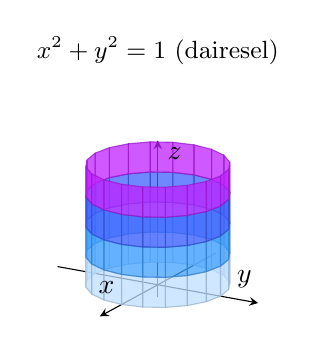
\begin{tikzpicture}
\begin{axis}[width=5.6cm,view={120}{25},axis lines=center,ticks=none,
  xlabel=$x$,ylabel=$y$,zlabel=$z$,colormap/cool,
  xmin=-1.6,xmax=1.6,ymin=-1.6,ymax=1.6,zmin=-0.2,zmax=2.4,
  title={\small $x^2+y^2=1$ (dairesel)}]
\addplot3[surf,shader=faceted,opacity=0.75,z buffer=sort,domain=0:360,y domain=0:2,samples=21,samples y=5]
  ({cos(x)},{sin(x)},{y});
\end{axis}
\end{tikzpicture}\qquad
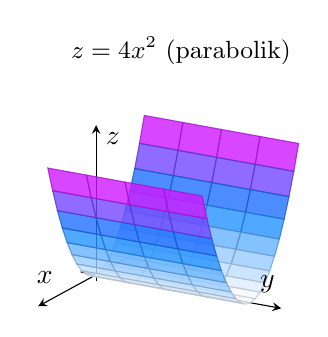
\begin{tikzpicture}
\begin{axis}[width=5.6cm,view={120}{25},axis lines=center,ticks=none,
  xlabel=$x$,ylabel=$y$,zlabel=$z$,colormap/cool,
  xmin=-1.2,xmax=1.2,ymin=-0.2,ymax=2.4,zmin=-0.2,zmax=4.5,
  title={\small $z=4x^2$ (parabolik)}]
\addplot3[surf,shader=faceted,opacity=0.8,domain=-1:1,y domain=0:2,samples=21,samples y=5]
  {4*x^2};
\end{axis}
\end{tikzpicture}
\end{center}

\begin{bilgi}[``Silindir'' kelimesi hakkında]
Günlük dilde ``silindir'' dairesel silindir demektir; matematikte ise dayanak eğrisi parabol, hiperbol, elips, hatta sinüs eğrisi olabilir. Örneğin $z=\sin y$ dalgalı bir oluk biçimli yüzeydir ($Ox$ eksenine paralel silindir). Düzlem de bir silindir sayılabilir: dayanak eğrisi doğru olan silindir.
\end{bilgi}

%======================================================================
\subsection{Kuadratik yüzeyler}

\begin{tanim}[Kuadratik (ikinci dereceden) yüzey]
$x,y,z$ cinsinden ikinci dereceden bir denklemin grafiğine \textbf{kuadratik yüzey} denir:
\[ Ax^2+By^2+Cz^2+Dxy+Exz+Fyz+Gx+Hy+Iz+J=0 . \]
Öteleme ve döndürme ile bu denklem standart biçimlerden birine getirilebilir. Bu derste karışık terimler ($xy$, $xz$, $yz$) olmayan durumla ilgileneceğiz; o zaman \emph{kareye tamamlama} (öteleme) yeterlidir.
\end{tanim}

\subsubsection{İzler (kesitler) yöntemi}

Bir yüzeyi kabaca çizmenin en etkili yolu, onu koordinat düzlemlerine paralel düzlemlerle kesip kesit eğrilerine (\textbf{izlere}) bakmaktır: $z=k$, $y=k$, $x=k$ düzlemleriyle arakesitler. Her iz, düzlemde tanıdığımız bir eğridir (elips, hiperbol, parabol, doğru çifti). Birkaç izi üst üste yerleştirince yüzeyin şekli ortaya çıkar.

\begin{tahta}[\foto{IMG-20261015-WA0043}]
Konu~4'teki $f(x,y)=x^2+y^2$ örneğinde $x^2+y^2=c$ seviye eğrileri $c=1,4,9$ için yarıçapları $1,2,3$ olan iç içe çemberler olarak çizilmiş, yanında da yatay çember kesitli $z=x^2+y^2$ yüzeyi gösterilmişti. Bu tam olarak izler yönteminin $z=k$ izleridir.
\end{tahta}
\begin{bilgi}[Çizim notu]
O fotoğraftaki yüzey düz kenarlarla, koni gibi çizilmiş. $z=x^2+y^2$ bir paraboloiddir; $x=0$ izi $z=y^2$ parabolü olduğu için kenarları \emph{eğridir} (kâse biçimi). Düz kenarlı yüzey $z=\sqrt{x^2+y^2}$ konisi olurdu.
\end{bilgi}

\begin{soru}[Örnek 15: izlerle tanıma]
$z=4x^2+y^2$ yüzeyinin izlerini bularak şeklini belirleyiniz.
\end{soru}
\begin{cevap}
\begin{itemize}
  \item $z=k$: $4x^2+y^2=k$. $k>0$ için elips ($\frac{x^2}{k/4}+\frac{y^2}{k}=1$), $k=0$ için yalnız orijin, $k<0$ için boş.
  \item $x=k$: $z=y^2+4k^2$, yukarı açılan parabol.
  \item $y=k$: $z=4x^2+k^2$, yukarı açılan parabol.
\end{itemize}
Yatay kesitler elips, dikey kesitler parabol $\Rightarrow$ tepe noktası orijinde, $Oz$ ekseni boyunca yukarı açılan \textbf{eliptik paraboloid}.
\end{cevap}

\subsubsection{Küre (kısaca)}

Konu~1'de gördüğümüz $M(a,b,c)$ merkezli, $r$ yarıçaplı küre $(x-a)^2+(y-b)^2+(z-c)^2=r^2$, aşağıdaki elipsoidin üç yarı ekseni eşit ($a=b=c=r$) olan özel hâlidir. Genel biçim $x^2+y^2+z^2+Dx+Ey+Fz+G=0$ kareye tamamlanarak merkez ve yarıçap bulunur; bütün kesitler çemberdir.

\subsubsection{Elipsoid}

\begin{tanim}[Elipsoid]
Koordinat düzlemleriyle arakesitleri elips olan yüzeye \textbf{elipsoid} denir:
\[ \frac{x^2}{a^2}+\frac{y^2}{b^2}+\frac{z^2}{c^2}=1\qquad(a,b,c>0). \]
\end{tanim}
\begin{itemize}
  \item Koordinat düzlemlerine göre simetriktir (her değişken kare olarak geçer); eksenleri $(\mp a,0,0)$, $(0,\mp b,0)$, $(0,0,\mp c)$ noktalarında keser.
  \item İzler: $z=k$ için $\frac{x^2}{a^2}+\frac{y^2}{b^2}=1-\frac{k^2}{c^2}$; $|k|<c$ ise elips, $|k|=c$ ise tek nokta, $|k|>c$ ise boş. Diğer izler de elipstir. Yüzey $|x|\le a$, $|y|\le b$, $|z|\le c$ kutusunun içindedir.
  \item $z$ çekilirse $z=\mp c\sqrt{1-\frac{x^2}{a^2}-\frac{y^2}{b^2}}$: $+$ işaret \textbf{üst yarı}, $-$ işaret \textbf{alt yarı} elipsoidi verir (her biri bir fonksiyon grafiğidir).
\end{itemize}

\begin{tahta}[\foto{IMG-20261015-WA0043}, \foto{IMG-20261023-WA0063}, \foto{IMG-20261022-WA0049}, \foto{IMG-20261108-WA0097}]
``Elipsoid: Koordinat düzlemleriyle arakesitleri elips olan yüzeylere denir. $\frac{x^2}{a^2}+\frac{y^2}{b^2}+\frac{z^2}{c^2}=1$. Bu yüzey koordinat düzlemlerine göre simetriktir; eksenleri $(\mp a,0,0)$, $(0,\mp b,0)$ ve $(0,0,\mp c)$ noktalarında keser. $z=c\sqrt{\cdots}$ üst elipsoid, $z=-c\sqrt{\cdots}$ alt elipsoid.''
(15.10 tahtasında ``koordinat düzlemine'' tekil yazılmıştı; doğrusu ``koordinat düzlemlerine''.)
\end{tahta}

\subsubsection{Hiperboloidler}

\begin{tanim}[Tek ve çift kanatlı hiperboloid]
\[ \textbf{Tek kanatlı:}\ \ \frac{x^2}{a^2}+\frac{y^2}{b^2}-\frac{z^2}{c^2}=1,\qquad
   \textbf{Çift kanatlı:}\ \ \frac{x^2}{a^2}+\frac{y^2}{b^2}-\frac{z^2}{c^2}=-1 . \]
Çift kanatlı olan $-\frac{x^2}{a^2}-\frac{y^2}{b^2}+\frac{z^2}{c^2}=1$ biçiminde de yazılır. Her ikisinde de \textbf{eksen}, işareti farklı olan değişkenin eksenidir (burada $Oz$).
\end{tanim}

\begin{tahta}[\foto{IMG-20261022-WA0049}, \foto{IMG-20261108-WA0097}, \foto{IMG-20261108-WA0096}]
``Bir hiperbolün yedek ekseni etrafında döndürülmesiyle tek kanatlı, asal ekseni etrafında döndürülmesiyle iki kanatlı hiperboloid elde edilir.'' Çizimler: kum saati biçimli tek kanatlı hiperboloid (``$z=0$'da elips, $x=0$'da hiperbol''); $z$ ekseni üzerinde biri yukarı biri aşağı açılan iki kâseden oluşan çift kanatlı hiperboloid (``$-c<z<c$ aralığında yüzey yok'').
\end{tahta}

\textbf{Tek kanatlı hiperboloidin izleri:} $z=k$ için $\frac{x^2}{a^2}+\frac{y^2}{b^2}=1+\frac{k^2}{c^2}$, \emph{her} $k$ için elips; en küçüğü $z=0$'daki ``bel'' elipsidir ve $|k|$ büyüdükçe büyür. $x=0$ için $\frac{y^2}{b^2}-\frac{z^2}{c^2}=1$ hiperbolü, $y=0$ için de hiperbol. Yüzey tek parçadır.

\textbf{Çift kanatlı hiperboloidin izleri:} $z=k$ için $\frac{x^2}{a^2}+\frac{y^2}{b^2}=\frac{k^2}{c^2}-1$; bu yalnız $|k|\ge c$ iken anlamlıdır. Bu yüzden $-c<z<c$ şeridinde yüzeyin hiçbir noktası yoktur; yüzey $z\ge c$ ve $z\le-c$ bölgelerinde iki ayrı parçadan (kanattan) oluşur, tepe noktaları $(0,0,\pm c)$'dir. $x=0$ ve $y=0$ izleri hiperboldür.

\textbf{Döndürme yorumu ($a=b$ iken):} $xz$-düzlemindeki $\frac{x^2}{a^2}-\frac{z^2}{c^2}=1$ hiperbolünün asal ekseni $Ox$, yedek (sanal) ekseni $Oz$'dir. Bu hiperbolü yedek ekseni $Oz$ etrafında döndürürsek $\frac{x^2+y^2}{a^2}-\frac{z^2}{c^2}=1$ tek kanatlı hiperboloidi; $\frac{z^2}{c^2}-\frac{x^2}{a^2}=1$ hiperbolünü asal ekseni $Oz$ etrafında döndürürsek çift kanatlı hiperboloidi elde ederiz. $a\neq b$ ise yüzeyler döndürme yüzeyi değildir ama şekil aynıdır.

\begin{center}
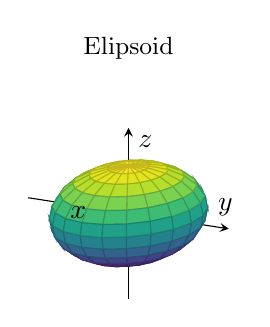
\begin{tikzpicture}
\begin{axis}[width=5.6cm,view={120}{20},axis lines=center,ticks=none,
  xlabel=$x$,ylabel=$y$,zlabel=$z$,colormap/viridis,
  xmin=-2.4,xmax=2.4,ymin=-2.4,ymax=2.4,zmin=-1.8,zmax=1.8,
  title={\small Elipsoid}]
\addplot3[surf,shader=faceted,z buffer=sort,domain=0:360,y domain=-90:90,samples=21,samples y=13]
  ({2*cos(y)*cos(x)},{1.5*cos(y)*sin(x)},{sin(y)});
\end{axis}
\end{tikzpicture}\qquad
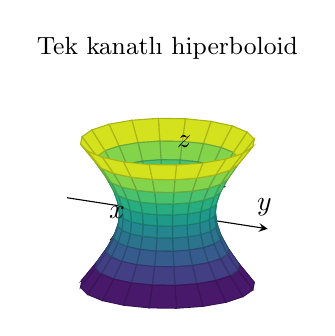
\begin{tikzpicture}
\begin{axis}[width=5.6cm,view={120}{20},axis lines=center,ticks=none,
  xlabel=$x$,ylabel=$y$,zlabel=$z$,colormap/viridis,
  xmin=-2.4,xmax=2.4,ymin=-2.4,ymax=2.4,zmin=-1.8,zmax=1.8,
  title={\small Tek kanatlı hiperboloid}]
\addplot3[surf,shader=faceted,z buffer=sort,domain=0:360,y domain=-1.2:1.2,samples=21,samples y=11]
  ({cosh(y)*cos(x)},{cosh(y)*sin(x)},{sinh(y)});
\end{axis}
\end{tikzpicture}
\end{center}
\begin{center}
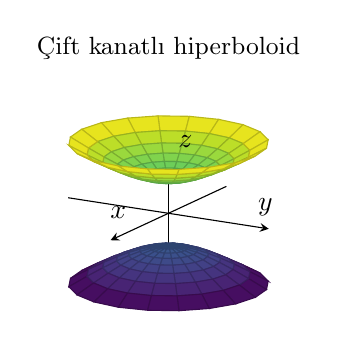
\begin{tikzpicture}
\begin{axis}[width=5.6cm,view={120}{20},axis lines=center,ticks=none,
  xlabel=$x$,ylabel=$y$,zlabel=$z$,colormap/viridis,
  xmin=-2.2,xmax=2.2,ymin=-2.2,ymax=2.2,zmin=-2.6,zmax=2.6,
  title={\small Çift kanatlı hiperboloid}]
\addplot3[surf,shader=faceted,z buffer=sort,domain=0:360,y domain=0:1.4,samples=21,samples y=9]
  ({sinh(y)*cos(x)},{sinh(y)*sin(x)},{cosh(y)});
\addplot3[surf,shader=faceted,z buffer=sort,domain=0:360,y domain=0:1.4,samples=21,samples y=9]
  ({sinh(y)*cos(x)},{sinh(y)*sin(x)},{-cosh(y)});
\end{axis}
\end{tikzpicture}\qquad
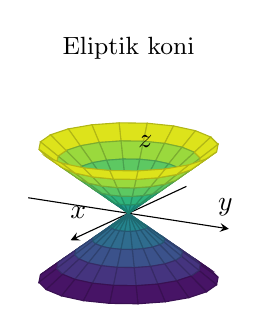
\begin{tikzpicture}
\begin{axis}[width=5.6cm,view={120}{20},axis lines=center,ticks=none,
  xlabel=$x$,ylabel=$y$,zlabel=$z$,colormap/viridis,
  xmin=-1.8,xmax=1.8,ymin=-1.8,ymax=1.8,zmin=-1.8,zmax=1.8,
  title={\small Eliptik koni}]
\addplot3[surf,shader=faceted,z buffer=sort,domain=0:360,y domain=-1.4:1.4,samples=21,samples y=11]
  ({y*cos(x)},{y*sin(x)},{y});
\end{axis}
\end{tikzpicture}
\end{center}

\subsubsection{Eliptik koni}

\begin{tanim}[Koni]
Sabit bir $T$ noktasından (tepe) geçen ve bir eğriyi kesen doğrunun hareketiyle oluşan yüzeye \textbf{koni} denir. Tepesi orijinde, ekseni $Oz$ olan eliptik koni:
\[ \frac{z^2}{c^2}=\frac{x^2}{a^2}+\frac{y^2}{b^2}\quad\Longrightarrow\quad z=\mp c\sqrt{\frac{x^2}{a^2}+\frac{y^2}{b^2}} . \]
$z=c\sqrt{\cdots}$ üst koni, $z=-c\sqrt{\cdots}$ alt konidir.
\end{tanim}
\begin{itemize}
  \item $z=k\neq0$: $\frac{x^2}{a^2}+\frac{y^2}{b^2}=\frac{k^2}{c^2}$ elips ($a=b$ ise çember); $k=0$: yalnız tepe noktası.
  \item $x=0$: $\frac{z^2}{c^2}=\frac{y^2}{b^2}$, yani $z=\pm\frac cb\,y$ \textbf{doğru çifti}; $y=0$ için de doğru çifti. $x=k\neq0$ izleri hiperboldür.
  \item Koni, tek ve çift kanatlı hiperboloidlerin ``arasındaki'' sınır durumudur: sağ taraf $1$, $0$, $-1$ olarak değişirken tek kanatlı hiperboloid $\to$ koni $\to$ çift kanatlı hiperboloid.
\end{itemize}

\begin{tahta}[\foto{IMG-20261022-WA0052}, \foto{IMG-20261108-WA0096}]
``Koni: Sabit bir $T$ noktasından geçen ve bir eğriyi kesen doğrunun oluşturduğu yüzeye denir. $\frac{z^2}{c^2}=\frac{x^2}{a^2}+\frac{y^2}{b^2}\to z=\mp c\sqrt{\frac{x^2}{a^2}+\frac{y^2}{b^2}}$.'' Çizim: tepe noktası orijinde, yukarı ve aşağı açılan çift koni ``(Tepe orijinde)''.
\end{tahta}

\subsubsection{Eliptik paraboloid}

\begin{tanim}[Eliptik paraboloid]
\[ z=\frac{x^2}{a^2}+\frac{y^2}{b^2}\qquad\text{(genel olarak } \tfrac{z}{c}=\tfrac{x^2}{a^2}+\tfrac{y^2}{b^2}\text{)} . \]
$z=k$ ($k>0$) düzlemleriyle arakesitleri elips olduğu için bu yüzeye \textbf{eliptik paraboloid} denir. $x=k$ ve $y=k$ izleri paraboldür. $c>0$ iken tepe noktası orijinde, yukarı açılan bir kâsedir.
\end{tanim}

\begin{tahta}[\foto{IMG-20261022-WA0050}, \foto{IMG-20261108-WA0096}]
``Parabolün simetri ekseni etrafında döndürülmesiyle elde edilen yüzeye paraboloid denir. Bu yüzeyin $z=c$ $(c>0)$ düzlemleriyle arakesiti bir elips olduğundan bu yüzeye eliptik paraboloid denir.'' (22.10 tahtasında başlık önce ``Hiper\ldots'' diye başlanıp düzeltilmiş ve ``Eliptoik'' diye yazılmıştı; doğrusu ``Eliptik''.)
\end{tahta}
\begin{bilgi}[Dönel paraboloid]
Bir parabolü simetri ekseni etrafında döndürmek, yalnızca $a=b$ olan \textbf{dönel paraboloidi} ($z=\frac{x^2+y^2}{a^2}$, yatay kesitleri çember) verir. $a\neq b$ iken yüzey bir döndürme yüzeyi değildir; kesitleri gerçek elipslerdir. Tahtadaki tanım bu nedenle önce dönel paraboloidi anlatıp sonra adı ``eliptik''e genişletiyor.
\end{bilgi}

\subsubsection{Hiperbolik paraboloid (eyer yüzeyi)}

\begin{tanim}[Hiperbolik paraboloid]
\[ \frac{z}{c}=\frac{x^2}{a^2}-\frac{y^2}{b^2}\qquad\text{(eyer / semer yüzeyi)}. \]
\end{tanim}
\begin{itemize}
  \item $z=k$: $\frac{x^2}{a^2}-\frac{y^2}{b^2}=\frac kc$ \textbf{hiperbol}ler ($k>0$ ve $k<0$ için farklı eksenlere açılır); $k=0$ için $y=\pm\frac ba x$ doğru çifti.
  \item $y=k$: $z=\frac{c}{a^2}x^2-\frac{ck^2}{b^2}$, yukarı açılan parabol ($c>0$).
  \item $x=k$: $z=\frac{ck^2}{a^2}-\frac{c}{b^2}y^2$, aşağı açılan parabol.
  \item Orijin bir \textbf{eyer noktasıdır}: $x$ yönünde yürüyünce orijin en alçak nokta, $y$ yönünde yürüyünce en yüksek noktadır. Bu nokta Konu~5--6'da ekstremum testlerinde tekrar karşımıza çıkacak.
\end{itemize}

\begin{tahta}[\foto{IMG-20261022-WA0052}, \foto{IMG-20261108-WA0095}]
``Hiperbolik paraboloid: $\frac zc=\frac{x^2}{a^2}-\frac{y^2}{b^2}$ (eyer yüzeyi).'' Tel kafes (ağ) biçiminde eyer çizimi.
(Bazı kitaplarda standart biçim $\frac zc=\frac{y^2}{b^2}-\frac{x^2}{a^2}$ olarak verilir; bu yalnızca yönelim farkıdır, yüzey aynı türdendir.)
\end{tahta}

\begin{center}
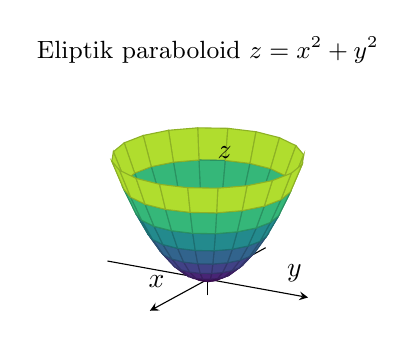
\begin{tikzpicture}
\begin{axis}[width=5.6cm,view={120}{25},axis lines=center,ticks=none,
  xlabel=$x$,ylabel=$y$,zlabel=$z$,colormap/viridis,
  xmin=-1.8,xmax=1.8,ymin=-1.8,ymax=1.8,zmin=-0.3,zmax=2.6,
  title={\small Eliptik paraboloid $z=x^2+y^2$}]
\addplot3[surf,shader=faceted,z buffer=sort,domain=0:360,y domain=0:1.5,samples=21,samples y=9]
  ({y*cos(x)},{y*sin(x)},{y^2});
\end{axis}
\end{tikzpicture}\qquad
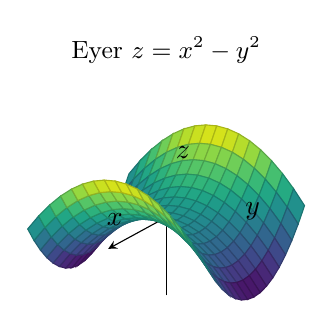
\begin{tikzpicture}
\begin{axis}[width=5.6cm,view={120}{25},axis lines=center,ticks=none,
  xlabel=$x$,ylabel=$y$,zlabel=$z$,colormap/viridis,
  xmin=-1.6,xmax=1.6,ymin=-1.6,ymax=1.6,zmin=-2.4,zmax=2.4,
  title={\small Eyer $z=x^2-y^2$}]
\addplot3[surf,shader=faceted,domain=-1.4:1.4,y domain=-1.4:1.4,samples=17]
  {x^2-y^2};
\end{axis}
\end{tikzpicture}
\end{center}

\subsubsection{Standart biçimler ve tanıma rehberi}

\begin{center}
\begin{tabular}{l l l}
\toprule
Yüzey & Standart denklem ($Oz$ ekseni) & İzler \\
\midrule
Elipsoid & $\frac{x^2}{a^2}+\frac{y^2}{b^2}+\frac{z^2}{c^2}=1$ & hepsi elips \\
Tek kanatlı hiperboloid & $\frac{x^2}{a^2}+\frac{y^2}{b^2}-\frac{z^2}{c^2}=1$ & $z=k$: elips; $x,y=k$: hiperbol \\
Çift kanatlı hiperboloid & $\frac{x^2}{a^2}+\frac{y^2}{b^2}-\frac{z^2}{c^2}=-1$ & $z=k$ ($|k|>c$): elips; diğer: hiperbol \\
Eliptik koni & $\frac{z^2}{c^2}=\frac{x^2}{a^2}+\frac{y^2}{b^2}$ & $z=k$: elips; $x,y=0$: doğru çifti \\
Eliptik paraboloid & $\frac{z}{c}=\frac{x^2}{a^2}+\frac{y^2}{b^2}$ & $z=k$: elips; $x,y=k$: parabol \\
Hiperbolik paraboloid & $\frac{z}{c}=\frac{x^2}{a^2}-\frac{y^2}{b^2}$ & $z=k$: hiperbol; $x,y=k$: parabol \\
Silindir & bir değişken eksik & eksik değişken yönünde sabit \\
\bottomrule
\end{tabular}
\end{center}

\begin{teorem}[Hızlı tanıma]
Denklemi (gerekirse kareye tamamlayarak) standart biçime getirin, sonra:
\begin{enumerate}
  \item Bir değişken hiç yoksa $\to$ \textbf{silindir} (o eksene paralel).
  \item Üç değişken de kare ve sabit terim var: hepsi aynı işaretli $\to$ \textbf{elipsoid}; biri farklı işaretli $\to$ \textbf{hiperboloid}. Hiperboloid için $=1$ biçiminde yazınca \emph{bir} eksi işaret varsa \textbf{tek kanatlı}, \emph{iki} eksi işaret varsa \textbf{çift kanatlı}dır. Eksen, işareti ``yalnız kalan'' değişkenin eksenidir.
  \item Üç değişken kare, sabit terim yok (sağ taraf $0$) ve işaretler karışık $\to$ \textbf{koni}.
  \item İki değişken kare, biri birinci dereceden $\to$ \textbf{paraboloid}: karelerin işaretleri aynıysa \textbf{eliptik}, farklıysa \textbf{hiperbolik}. Eksen, birinci dereceden değişkenin eksenidir.
\end{enumerate}
\end{teorem}

\subsubsection{Genel kuadratik denklemi kareye tamamlayarak tanıma}

\begin{bilgi}[Derste tahtada görülmedi, kaynaklardan eklendi]
Karışık terimi olmayan $Ax^2+By^2+Cz^2+Gx+Hy+Iz+J=0$ denkleminde her değişken için kareye tamamlanır: $x^2-2px=(x-p)^2-p^2$. Böylece yüzey, merkezi/tepesi $(p,q,r)$ noktasına ötelenmiş bir standart yüzey olarak tanınır (Konu~1'de küre denkleminde yaptığımız işlemin aynısı).
\end{bilgi}

\begin{soru}[Örnek 16 (kaynaklardan)]
$x^2+2z^2-6x-y+10=0$ yüzeyini tanıyınız.
\end{soru}
\begin{cevap}
$x$ için kareye tamamlayalım: $x^2-6x=(x-3)^2-9$. Denklem
\[ (x-3)^2-9+2z^2-y+10=0\ \Longrightarrow\ y-1=(x-3)^2+2z^2 . \]
İki değişken ($x$, $z$) kare ve aynı işaretli, $y$ birinci dereceden $\Rightarrow$ \textbf{eliptik paraboloid}. Tepe noktası $(3,1,0)$, ekseni $Oy$'ye paralel ($x=3,\ z=0$ doğrusu), $+y$ yönünde açılır. $y=k$ ($k>1$) izleri $(x-3)^2+2z^2=k-1$ elipsleridir.
\end{cevap}

\begin{soru}[Örnek 17 (kaynaklardan)]
$x^2+y^2-z^2-4x+6y+2z+8=0$ yüzeyini tanıyınız.
\end{soru}
\begin{cevap}
Kareye tamamlama: $x^2-4x=(x-2)^2-4$, $y^2+6y=(y+3)^2-9$, $-(z^2-2z)=-(z-1)^2+1$. Yerine yazarsak
\[ (x-2)^2-4+(y+3)^2-9-(z-1)^2+1+8=0\ \Longrightarrow\ (x-2)^2+(y+3)^2-(z-1)^2=4, \]
\[ \frac{(x-2)^2}{4}+\frac{(y+3)^2}{4}-\frac{(z-1)^2}{4}=1 . \]
Sağ taraf $1$ iken \emph{bir} eksi işaret $\Rightarrow$ \textbf{tek kanatlı hiperboloid}; merkezi $(2,-3,1)$, ekseni $Oz$'ye paralel. $a=b=2$ olduğundan dönel hiperboloiddir; bel çemberi $z=1$ düzleminde, yarıçapı $2$.
\end{cevap}

%======================================================================
\subsection{Kaynak kitaplardan ek örnekler}

\begin{soru}[\ekal Ek örnek 1: aykırı doğrular]
$d_1:\ x=1+t,\ y=-2+3t,\ z=4-t$ ve $d_2:\ x=2s,\ y=3+s,\ z=-3+4s$ doğrularının paralel, kesişen ya da aykırı olduğunu belirleyiniz; aykırı ise aralarındaki uzaklığı bulunuz.
\end{soru}
\begin{cevap}
Doğrultmanlar $\mathbf v=(1,3,-1)$, $\mathbf u=(2,1,4)$; oranlar $\frac12\neq\frac31$ olduğundan paralel değiller.

Kesişme: $1+t=2s$ ve $-2+3t=3+s$. İlkinden $t=2s-1$; ikincide $-2+6s-3=3+s\Rightarrow5s=8$, $s=\frac85$, $t=\frac{11}{5}$. Üçüncü bileşen: $4-t=\frac95$, $-3+4s=\frac{17}{5}$; eşit değil $\Rightarrow$ kesişmezler. Doğrular \textbf{aykırıdır}.

Uzaklık: $P_1(1,-2,4)$, $P_2(0,3,-3)$, $\overrightarrow{P_1P_2}=(-1,5,-7)$.
\[ \mathbf v\times\mathbf u=\begin{vmatrix}\mathbf i&\mathbf j&\mathbf k\\1&3&-1\\2&1&4\end{vmatrix}=(12+1,\ -(4+2),\ 1-6)=(13,-6,-5), \]
\[ d=\frac{|(-1)(13)+5(-6)+(-7)(-5)|}{\sqrt{169+36+25}}=\frac{|-13-30+35|}{\sqrt{230}}=\frac{8}{\sqrt{230}}\approx0{,}53 . \]
\end{cevap}

\begin{soru}[\ekal Ek örnek 2: kesişen doğrular]
$d_1:\ x=1+t,\ y=2-t,\ z=3+2t$ ve $d_2:\ x=1+s,\ y=-1+2s,\ z=6-s$ doğrularının kesişip kesişmediğini belirleyiniz; kesişiyorlarsa kesim noktasını ve aralarındaki açıyı bulunuz.
\end{soru}
\begin{cevap}
$x$: $1+t=1+s\Rightarrow t=s$. $y$: $2-t=-1+2s=-1+2t\Rightarrow t=1$, $s=1$. $z$: $3+2(1)=5$ ve $6-1=5$ \checkmark. Doğrular \textbf{kesişir}; kesim noktası $(2,1,5)$.

Açı: $\mathbf v=(1,-1,2)$, $\mathbf u=(1,2,-1)$, $\mathbf v\cdot\mathbf u=1-2-2=-3$, $\|\mathbf v\|=\|\mathbf u\|=\sqrt6$:
$\cos\theta=\frac{|-3|}{6}=\frac12\Rightarrow\theta=60^\circ$.
\end{cevap}

\begin{soru}[\ekal Ek örnek 3: düzlemler arası açı]
$x+y+z=1$ ve $x-2y+3z=1$ düzlemleri arasındaki açıyı bulunuz.
\end{soru}
\begin{cevap}
$\mathbf n_1=(1,1,1)$, $\mathbf n_2=(1,-2,3)$, $\mathbf n_1\cdot\mathbf n_2=1-2+3=2$, $\|\mathbf n_1\|=\sqrt3$, $\|\mathbf n_2\|=\sqrt{14}$:
\[ \cos\theta=\frac{2}{\sqrt3\sqrt{14}}=\frac{2}{\sqrt{42}}\approx0{,}309\ \Rightarrow\ \theta\approx72^\circ . \]
\end{cevap}

\begin{soru}[\ekal Ek örnek 4: paralel düzlemler arası uzaklık]
$10x+2y-2z=5$ ve $5x+y-z=1$ düzlemleri arasındaki uzaklığı bulunuz.
\end{soru}
\begin{cevap}
Normaller $(10,2,-2)=2(5,1,-1)$; düzlemler paralel. Formülü kullanmak için \emph{aynı katsayılarla} yazalım: ikinci denklemi $2$ ile çarparsak $10x+2y-2z-2=0$; birincisi $10x+2y-2z-5=0$. Böylece $D_1=-5$, $D_2=-2$:
\[ d=\frac{|D_2-D_1|}{\sqrt{100+4+4}}=\frac{3}{\sqrt{108}}=\frac{3}{6\sqrt3}=\frac{\sqrt3}{6}\approx0{,}289 . \]
(Kontrol: birinci düzlemden $K(\frac12,0,0)$ alıp ikinciye uzaklığı: $\frac{|5/2-1|}{\sqrt{27}}=\frac{3/2}{3\sqrt3}=\frac{\sqrt3}{6}$ \checkmark.)
\end{cevap}

\begin{soru}[\ekal Ek örnek 5: iki düzleme paralel doğru]
$P(1,-1,2)$ noktasından geçen ve $x+y-z=1$ ile $2x-y+3z=4$ düzlemlerinin ikisine de paralel olan doğrunun denklemini yazınız.
\end{soru}
\begin{cevap}
Doğru her iki düzleme paralelse doğrultmanı iki normale de diktir: $\mathbf v=\mathbf n_1\times\mathbf n_2$.
\[ \mathbf v=\begin{vmatrix}\mathbf i&\mathbf j&\mathbf k\\1&1&-1\\2&-1&3\end{vmatrix}=\big(3-1,\ -(3+2),\ -1-2\big)=(2,-5,-3). \]
\[ \frac{x-1}{2}=\frac{y+1}{-5}=\frac{z-2}{-3}. \]
Kontrol: $\mathbf v\cdot\mathbf n_1=2-5+3=0$, $\mathbf v\cdot\mathbf n_2=4+5-9=0$ \checkmark.
\end{cevap}

\begin{soru}[\ekal Ek örnek 6: silindiri tanıma]
$y^2+z^2=9$ ve $x=y^2$ yüzeylerini tanıyınız.
\end{soru}
\begin{cevap}
$y^2+z^2=9$ denkleminde $x$ yok $\Rightarrow$ $Ox$ eksenine paralel silindir; dayanak eğrisi $yz$-düzleminde yarıçapı $3$ olan çember: ekseni $Ox$ olan \textbf{dairesel silindir}.

$x=y^2$ denkleminde $z$ yok $\Rightarrow$ $Oz$'ye paralel silindir; dayanak eğrisi $xy$-düzleminde $x=y^2$ parabolü: \textbf{parabolik silindir} (dikey duran bir oluk).
\end{cevap}

\begin{soru}[\ekal Ek örnek 7: çift kanatlı hiperboloid]
$4x^2-y^2+2z^2+4=0$ yüzeyini tanıyınız.
\end{soru}
\begin{cevap}
$-4$'e bölersek $-x^2+\frac{y^2}{4}-\frac{z^2}{2}=1$. Sağ taraf $1$ iken \emph{iki} eksi işaret $\Rightarrow$ \textbf{çift kanatlı hiperboloid}; yalnız kalan pozitif değişken $y$ olduğundan ekseni $Oy$'dir. $y=k$ izleri $x^2+\frac{z^2}{2}=\frac{k^2}{4}-1$, yalnız $|k|\ge2$ için var: yüzey $-2<y<2$ şeridinde boştur, tepe noktaları $(0,\pm2,0)$.
\end{cevap}

%======================================================================
\subsection{Sık yapılan hatalar}

\begin{dikkat}
\begin{itemize}
  \item \textbf{Uzayda doğruyu tek denklemle yazmak.} $3x-2y+1=0$ uzayda bir düzlemdir; doğru için iki denklem (ya da parametrik/kartezyen biçim) gerekir (Örnek~1).
  \item \textbf{Paydada sıfıra bölmek.} Doğrultman parametresi $0$ ise o değişken sabittir: $\mathbf v=(2,3,0)$ ise $z=z_0$ yazılır.
  \item \textbf{Normal ile doğrultmanı karıştırmak.} Düzlemin $x,y,z$ katsayıları \emph{normaldir}, doğrunun paydaları \emph{doğrultmandır}. Doğru düzleme dikse $\mathbf v\parallel\mathbf n$, paralelse $\mathbf v\perp\mathbf n$ (tersini yazmak çok yaygın bir hatadır).
  \item \textbf{Doğrunun noktasını yanlış işaretle almak.} $\frac{z+1}{6}$ ifadesinde $z_0=-1$'dir, $+1$ değil.
  \item \textbf{Paralel düzlem uzaklığını katsayıları eşitlemeden hesaplamak.} $|D_2-D_1|$ formülü yalnız $A,B,C$ aynı iken geçerlidir (Ek örnek 4).
  \item \textbf{$D$'yi yanlış taraftan okumak.} $2x+2y+2z=5$ için $D=-5$'tir; önce $Ax+By+Cz+D=0$ biçimine getirin.
  \item \textbf{Açıda mutlak değeri unutmak.} Doğrular/düzlemler arası açı istenirken dar açı verilir; $\cos\theta<0$ çıkarsa $180^\circ-\theta$ alın.
  \item \textbf{Paralellik testini $aA+bB+cC=0$ ile bitirmek.} Doğru düzlemin içinde de olabilir; bir noktasını düzlemde deneyin.
  \item \textbf{Sağlama yapmamak.} Bulunan düzlemin verilen noktalardan geçtiğini, kesim noktasının hem doğruyu hem düzlemi sağladığını kontrol edin (Örnek~7'deki tahta hatası böyle yakalanır).
  \item \textbf{Hiperboloidleri karıştırmak.} $=1$ biçiminde bir eksi: tek kanatlı; iki eksi: çift kanatlı. Sağ taraf $0$ ise koni.
  \item \textbf{Paraboloidi koni gibi çizmek.} $z=x^2+y^2$ kâse biçimlidir; $z=\sqrt{x^2+y^2}$ konidir.
\end{itemize}
\end{dikkat}

%======================================================================
\subsection{Özet ve formül kutusu}

\begin{ozet}
\textbf{Doğru} ($A(x_0,y_0,z_0)$, $\mathbf v=(a,b,c)$):
\[ \overrightarrow{AP}=t\mathbf v;\quad x=x_0+at,\ y=y_0+bt,\ z=z_0+ct;\quad \frac{x-x_0}{a}=\frac{y-y_0}{b}=\frac{z-z_0}{c}. \]
$b=0$ ise $y=y_0$, $\frac{x-x_0}{a}=\frac{z-z_0}{c}$. İki noktadan geçen doğru: $\mathbf v=\overrightarrow{AB}$.

\textbf{İki doğru} ($\mathbf v=(a,b,c)$, $\mathbf u=(p,q,r)$): paralel $\frac ap=\frac bq=\frac cr$; dik $ap+bq+cr=0$;
$\cos\theta=\frac{|\mathbf u\cdot\mathbf v|}{\|\mathbf u\|\|\mathbf v\|}$; aykırı uzaklık $\frac{|\overrightarrow{P_1P_2}\cdot(\mathbf v\times\mathbf u)|}{\|\mathbf v\times\mathbf u\|}$.

\textbf{Nokta--doğru uzaklığı:} $\ell=\dfrac{\|\overrightarrow{AP}\times\mathbf v\|}{\|\mathbf v\|}$.

\textbf{Düzlem} ($P_0$, $\mathbf n=(A,B,C)$): $A(x-x_0)+B(y-y_0)+C(z-z_0)=0$, $Ax+By+Cz+D=0$.
Üç nokta: $\mathbf n=\overrightarrow{AB}\times\overrightarrow{AC}$ (determinant $=0$). Doğruya dik düzlem: $\mathbf n=\mathbf v$.

\textbf{İki düzlem:} paralel $\frac{A_1}{A_2}=\frac{B_1}{B_2}=\frac{C_1}{C_2}$ ($\neq\frac{D_1}{D_2}$); çakışık ($=\frac{D_1}{D_2}$); dik $A_1A_2+B_1B_2+C_1C_2=0$;
$\cos\theta=\frac{|\mathbf n_1\cdot\mathbf n_2|}{\|\mathbf n_1\|\|\mathbf n_2\|}$; arakesit doğrultmanı $\mathbf n_1\times\mathbf n_2$.

\textbf{Doğru--düzlem:} dik $\frac aA=\frac bB=\frac cC$; paralel (veya içinde) $aA+bB+cC=0$; $\sin\varphi=\frac{|\mathbf v\cdot\mathbf n|}{\|\mathbf v\|\|\mathbf n\|}$; kesim noktası: parametrik denklemi düzlemde yerine koy.

\textbf{Uzaklıklar:}
\[ d(P,\text{düzlem})=\frac{|Ax_0+By_0+Cz_0+D|}{\sqrt{A^2+B^2+C^2}},\qquad d(P_1,P_2)=\frac{|D_2-D_1|}{\sqrt{A^2+B^2+C^2}}. \]

\textbf{Silindir:} bir değişken eksik $\Rightarrow$ o eksene paralel silindir.

\textbf{Kuadratik yüzeyler} ($Oz$ ekseni):
\begin{center}
\begin{tabular}{l l}
\toprule
Elipsoid & $\frac{x^2}{a^2}+\frac{y^2}{b^2}+\frac{z^2}{c^2}=1$\\
Tek kanatlı hiperboloid & $\frac{x^2}{a^2}+\frac{y^2}{b^2}-\frac{z^2}{c^2}=1$\\
Çift kanatlı hiperboloid & $\frac{x^2}{a^2}+\frac{y^2}{b^2}-\frac{z^2}{c^2}=-1$\\
Eliptik koni & $\frac{z^2}{c^2}=\frac{x^2}{a^2}+\frac{y^2}{b^2}$\\
Eliptik paraboloid & $\frac zc=\frac{x^2}{a^2}+\frac{y^2}{b^2}$\\
Hiperbolik paraboloid (eyer) & $\frac zc=\frac{x^2}{a^2}-\frac{y^2}{b^2}$\\
\bottomrule
\end{tabular}
\end{center}
Tanıma: kareye tamamla $\to$ işaretleri say $\to$ izlere bak.
\end{ozet}

\clearpage\section{Vektör Fonksiyonları ve Uzay Eğrileri}

\subsection{Amaç ve sezgi}

İlk iki konuda \emph{sabit} nesnelerle çalıştık: vektörler, doğrular, düzlemler ve yüzeyler. Oysa mühendislikte
ilgilendiğimiz şeylerin çoğu \emph{hareket eder}: bir uçağın rotası, bir robot kolunun ucu, raylı sistemde bir vagon,
bir CNC tezgâhında kesici takımın izlediği yol, Güneş etrafında dönen bir uydu\dots{} Bu cisimlerin her birinin $t$
anındaki konumu uzayda bir noktadır; o noktayı orijine bağlayan vektöre \textbf{konum (yer) vektörü} denir ve zamana bağlı
olduğu için $\mathbf r(t)$ ile gösterilir. $t$ değiştikçe $\mathbf r(t)$ vektörünün ucu uzayda bir \textbf{eğri} çizer.

Bu konunun bütün fikri şu basit gözleme dayanır: \vurg{bir vektör fonksiyonu, üç tane sıradan reel fonksiyonun yan yana
yazılmasıdır.} Bu yüzden limit, süreklilik, türev ve integral gibi Analiz~I'den bildiğimiz işlemlerin hepsi
\emph{bileşen bileşen} yapılır. Yeni olan, bu sonuçların \emph{geometrik ve fiziksel anlamıdır}:

\begin{center}
\begin{tabular}{l l}
\toprule
Matematiksel nesne & Geometrik / fiziksel anlamı \\
\midrule
$\mathbf r(t)$ & konum; ucu eğriyi çizer \\
$\mathbf r'(t)$ & teğet vektör; hız vektörü $\mathbf v(t)$ \\
$\|\mathbf r'(t)\|$ & sürat (hızın büyüklüğü), $ds/dt$ \\
$\mathbf r''(t)$ & ivme vektörü $\mathbf a(t)$ \\
$\int_a^b\|\mathbf r'(t)\|\,dt$ & yay uzunluğu (alınan yol) \\
$\mathbf T,\ \mathbf N,\ \mathbf B$ & eğri boyunca hareket eden ``yerel eksen takımı'' (Frenet çatısı) \\
$\kappa$ (eğrilik) & eğrinin ne kadar keskin döndüğü \\
$\tau$ (burulma) & eğrinin düzlemden ne kadar ``kıvrılıp çıktığı'' \\
\bottomrule
\end{tabular}
\end{center}

\begin{bilgi}[Bu konunun kaynakları ve gösterim]
Bu bölüm üç ayrı not kümesine dayanır: \textbf{09.10} tarihli defter sayfaları, \textbf{15.10} tarihli defter sayfaları ve
\textbf{23.10} tarihli tahta fotoğrafları. Aynı örnekler bu kümelerde tekrar ettiği için her örnek bir kez yazılmış,
bütün fotoğraf kaynakları başlıkta verilmiştir. Kaynak kitaplar: Kreyszig (\emph{Advanced Engineering Mathematics}),
Zill \& Wright (\emph{Calculus}, çev. Cangül), Balcı (\emph{Genel Matematik II}).

Gösterim: $\mathbf i=(1,0,0)$, $\mathbf j=(0,1,0)$, $\mathbf k=(0,0,1)$ standart birim vektörlerdir;
$f(t)\mathbf i+g(t)\mathbf j+h(t)\mathbf k$ ile $(f(t),g(t),h(t))$ aynı vektörü gösterir. Tahtada hız vektörü bazen
$V$, bazen $\mathbf v$ ile; sürat (hızın büyüklüğü) ise $\upsilon$ ile gösterilmiştir. $\|\cdot\|$ vektörün normudur (uzunluğu).
\end{bilgi}

%======================================================================
\subsection{Vektör değerli fonksiyonlar ve işlemler}

\subsubsection{Tanım ve bileşen fonksiyonlar}

Analiz~I'de $f:A\to\mathbb R$ ($A\subset\mathbb R$) biçiminde, bir sayıya bir sayı karşılık getiren fonksiyonlarla
çalıştık. Şimdi bir sayıya (genellikle zamana) bir \emph{vektör} karşılık getiren fonksiyonlara bakıyoruz.

\begin{tahta}[\foto{IMG-20261009-WA0016}, \foto{IMG-20261023-WA0034}]
Bir cismin $t$ anındaki konumu uzayda bir nokta: $P\big(x(t),y(t),z(t)\big)$. $x=f(t)$, $y=g(t)$, $z=h(t)$ ise yer vektörü
\[ \mathbf r(t)=f(t)\,\mathbf i+g(t)\,\mathbf j+h(t)\,\mathbf k . \]
$t$ aralığı taradığında $\mathbf r(t)$'nin ucu bir eğri çizer.
\end{tahta}

\begin{tanim}[Vektör değerli fonksiyon]
$I\subset\mathbb R$ bir aralık, $V$ (üç boyutlu uzaydaki, $E^3$) vektörlerin kümesi olsun. $\mathbf F:I\to V$ fonksiyonuna
\textbf{vektör değerli fonksiyon} denir:
\[ \mathbf F(t)=f(t)\,\mathbf i+g(t)\,\mathbf j+h(t)\,\mathbf k=\big(f(t),\,g(t),\,h(t)\big). \]
Reel değerli $f,g,h$ fonksiyonlarına $\mathbf F$'nin \textbf{bileşen fonksiyonları} denir.
\end{tanim}

Düzlemde çalışıyorsak $\mathbf k$ bileşeni yoktur: $\mathbf F(t)=f(t)\mathbf i+g(t)\mathbf j$. Örneğin
$\mathbf r(t)=\cos t\,\mathbf i+\sin t\,\mathbf j$ birim çemberi, $\mathbf r(t)=t\,\mathbf i+t^2\mathbf j+t^3\mathbf k$ ise
uzayda ``bükülmüş kübik'' denen eğriyi verir.

\subsubsection{Tanım kümesi}

\begin{teorem}[En geniş tanım kümesi]
Tanım kümesi ayrıca belirtilmemişse, $\mathbf F$'nin en geniş tanım kümesi bileşenlerinin tanım kümelerinin arakesitidir:
\[ T_{\mathbf F}=T_f\cap T_g\cap T_h . \]
\end{teorem}

Mantığı açıktır: $\mathbf F(t)$ vektörünün tanımlı olması için \emph{üç bileşenin birden} tanımlı olması gerekir.

\begin{soru}[Örnek 1 \foto{IMG-20261009-WA0016}, \foto{IMG-20261023-WA0060}]
$\mathbf F(t)=(t+1)\,\mathbf i+\ln(1-t)\,\mathbf j+\sqrt{4-t^2}\,\mathbf k$ fonksiyonunun tanım kümesini bulunuz.
\end{soru}
\begin{cevap}
Her bileşenin tanım kümesini ayrı ayrı bulup kesiştiririz.
\begin{itemize}
\item $f(t)=t+1$ bir polinom: $T_f=(-\infty,+\infty)$.
\item $g(t)=\ln(1-t)$: logaritmanın içi pozitif olmalı, $1-t>0\Rightarrow t<1$: $T_g=(-\infty,1)$.
\item $h(t)=\sqrt{4-t^2}$: karekökün içi negatif olmamalı, $4-t^2\ge 0\Rightarrow -2\le t\le 2$: $T_h=[-2,2]$.
\end{itemize}
Sayı doğrusunda bu üç kümenin ortak kısmı $-2$'den (dahil) $1$'e (hariç) kadardır:
\[ T_{\mathbf F}=(-\infty,+\infty)\cap(-\infty,1)\cap[-2,2]=\boxed{[-2,1)} . \]
$t=1$ dışarıda kalır, çünkü $\ln 0$ tanımsızdır; $t=-2$ içeride kalır, çünkü $\sqrt{0}=0$ tanımlıdır.
\end{cevap}

\subsubsection{Vektör fonksiyonlarla işlemler}

\begin{tanim}[İşlemler]
$\mathbf F,\mathbf G$ vektör değerli, $f,g$ reel değerli fonksiyonlar olsun. Ortak tanım kümesinde
\begin{enumerate}
\item $(\mathbf F+\mathbf G)(t)=\mathbf F(t)+\mathbf G(t)$
\item $(\mathbf F-\mathbf G)(t)=\mathbf F(t)-\mathbf G(t)$
\item $(\mathbf F\cdot\mathbf G)(t)=\mathbf F(t)\cdot\mathbf G(t)$ \quad (skaler çarpım: sonuç \emph{reel} fonksiyon)
\item $(\mathbf F\times\mathbf G)(t)=\mathbf F(t)\times\mathbf G(t)$ \quad (vektörel çarpım: sonuç \emph{vektör} fonksiyon)
\item $(f\mathbf G)(t)=f(t)\,\mathbf G(t)$ \quad (skalerle çarpım)
\item $(\mathbf F\circ g)(t)=\mathbf F\big(g(t)\big)$ \quad (bileşke)
\end{enumerate}
\end{tanim}

Yani her $t$ değeri için Konu~1'de öğrendiğimiz vektör işlemlerini yapıyoruz; sonuç yine $t$'nin bir fonksiyonu oluyor.

\begin{soru}[Örnek 2 \foto{IMG-20261009-WA0017}, \foto{IMG-20261023-WA0060}, \foto{IMG-20261023-WA0035}]
$\mathbf F(t)=t\,\mathbf i+t^2\mathbf j+t^3\mathbf k$, $\mathbf G(t)=(1-t)\,\mathbf i+(1+t^2)\,\mathbf j+t\,\mathbf k$,
$f(t)=t+1$, $g(t)=t-2$ olsun. $\mathbf F+\mathbf G$, $\mathbf F\cdot\mathbf G$, $\mathbf F\times\mathbf G$, $f\mathbf G$
ve $\mathbf F\circ g$ fonksiyonlarını bulunuz.
\end{soru}
\begin{cevap}
\textbf{1) Toplam} (karşılıklı bileşenler toplanır):
\[ (\mathbf F+\mathbf G)(t)=(t+1-t)\,\mathbf i+(t^2+1+t^2)\,\mathbf j+(t^3+t)\,\mathbf k=\mathbf i+(2t^2+1)\,\mathbf j+(t^3+t)\,\mathbf k . \]
\textbf{2) Skaler çarpım} (karşılıklı bileşenler çarpılıp toplanır; sonuç bir sayı fonksiyonu):
\[ (\mathbf F\cdot\mathbf G)(t)=t(1-t)+t^2(1+t^2)+t^3\cdot t=t-t^2+t^2+t^4+t^4=2t^4+t . \]
\textbf{3) Vektörel çarpım} (determinant ile, birinci satıra göre açılım):
\begin{align*}
(\mathbf F\times\mathbf G)(t)&=\begin{vmatrix}\mathbf i&\mathbf j&\mathbf k\\ t&t^2&t^3\\ 1-t&1+t^2&t\end{vmatrix}\\
&=\mathbf i\big(t^2\cdot t-t^3(1+t^2)\big)-\mathbf j\big(t\cdot t-t^3(1-t)\big)+\mathbf k\big(t(1+t^2)-t^2(1-t)\big)\\
&=-t^5\,\mathbf i-(t^4-t^3+t^2)\,\mathbf j+(2t^3-t^2+t)\,\mathbf k .
\end{align*}
\textbf{4) Skalerle çarpım} ($f(t)$ her bileşene dağıtılır):
\[ (f\mathbf G)(t)=(t+1)\big[(1-t)\mathbf i+(1+t^2)\mathbf j+t\,\mathbf k\big]=(1-t^2)\,\mathbf i+(t^3+t^2+t+1)\,\mathbf j+(t^2+t)\,\mathbf k . \]
\textbf{5) Bileşke} ($\mathbf F$'de $t$ yerine $g(t)=t-2$ yazılır):
\[ (\mathbf F\circ g)(t)=\mathbf F(t-2)=(t-2)\,\mathbf i+(t-2)^2\,\mathbf j+(t-2)^3\,\mathbf k . \]
\textbf{Kontrol:} Vektörel çarpım her iki çarpana da dik olmalıdır. Örneğin $t=1$'de $\mathbf F=(1,1,1)$,
$\mathbf F\times\mathbf G=(-1,-1,2)$ ve $(1,1,1)\cdot(-1,-1,2)=0$ \checkmark
\end{cevap}

\begin{bilgi}[Not]
23.10 tahta fotoğrafında (\foto{IMG-20261023-WA0035}) işlemler listesinin sağ kısmı hocanın arkasında kalmıştır;
eksik kalan kısım 09.10 defter sayfasından (\foto{IMG-20261009-WA0017}) tamamlanmıştır. Tahtadaki toplamda $\mathbf i$
bileşeni $(t+1-t)$ diye bırakılmış, sadeleşince $1$ olur.
\end{bilgi}

\subsubsection{Ortogonal (dik) fonksiyonlar}

\begin{tanim}[Ortogonal fonksiyonlar]
$\mathbf F$ ve $\mathbf G$ bir $I$ aralığında tanımlı olsun. \textbf{Her} $t\in I$ için $\mathbf F(t)\cdot\mathbf G(t)=0$ ise
$\mathbf F$ ile $\mathbf G$ \textbf{ortogonaldir} (diktir).
\end{tanim}

Dikkat: Tanım ``her $t$ için'' der. $\mathbf F(t)\cdot\mathbf G(t)$ yalnızca bazı $t$ değerlerinde sıfır oluyorsa
fonksiyonlar ortogonal değildir; sadece o anlarda vektörler diktir. (Örneğin $\mathbf F=\mathbf i$, $\mathbf G=t\,\mathbf i+\mathbf j$ için
$\mathbf F\cdot\mathbf G=t$ yalnız $t=0$'da sıfırdır.)

\begin{soru}[Örnek 3 \foto{IMG-20261009-WA0017}, \foto{IMG-20261023-WA0035}]
$\mathbf F(t)=(t+t^2)\,\mathbf i+2t\,\mathbf j-4t\,\mathbf k$ ve $\mathbf G(t)=(2+4t)\,\mathbf i+(1-3t)\,\mathbf j+(1+t^2)\,\mathbf k$
fonksiyonları ortogonal midir?
\end{soru}
\begin{cevap}
Skaler çarpımı hesaplayıp her $t$ için sıfır olup olmadığına bakarız:
\begin{align*}
\mathbf F(t)\cdot\mathbf G(t)&=(t+t^2)(2+4t)+2t(1-3t)+(-4t)(1+t^2)\\
&=(2t+6t^2+4t^3)+(2t-6t^2)+(-4t-4t^3)\\
&=(2t+2t-4t)+(6t^2-6t^2)+(4t^3-4t^3)=0 .
\end{align*}
Sonuç $t$'den bağımsız olarak sıfır olduğundan $\mathbf F$ ve $\mathbf G$ \textbf{ortogonaldir}.
\end{cevap}

\subsubsection{Norm}

\begin{tanim}[Norm]
$\mathbf F(t)=f(t)\mathbf i+g(t)\mathbf j+h(t)\mathbf k$ için
\[ \|\mathbf F(t)\|=\sqrt{\big(f(t)\big)^2+\big(g(t)\big)^2+\big(h(t)\big)^2} \]
reel değerli fonksiyonuna $\mathbf F$'nin \textbf{normu} denir. $\mathbf F$ bir konum vektörü ise $\|\mathbf F(t)\|$,
$t$ anında cismin orijine uzaklığıdır.
\end{tanim}

\begin{soru}[Örnek 4 \foto{IMG-20261009-WA0018}, \foto{IMG-20261023-WA0035}, \foto{IMG-20261023-WA0046}]
$\mathbf F(t)=2\cos t\,\mathbf i+2\sin t\,\mathbf j+3t\,\mathbf k$ fonksiyonunun normunu bulunuz.
\end{soru}
\begin{cevap}
\[ \|\mathbf F(t)\|=\sqrt{4\cos^2t+4\sin^2t+9t^2}=\sqrt{4(\cos^2t+\sin^2t)+9t^2}=\sqrt{4+9t^2}, \]
çünkü $\sin^2t+\cos^2t=1$. (Bu eğri bir helistir; $t$ büyüdükçe orijinden uzaklaşır.)
\end{cevap}

%======================================================================
\subsection{Limit ve süreklilik}

\subsubsection{Limit}

\begin{tanim}[Limit]
Her $\varepsilon>0$ için, $0<|t-t_0|<\delta$ iken $\|\mathbf F(t)-\mathbf L\|<\varepsilon$ olacak şekilde bir $\delta>0$
bulunabiliyorsa $\mathbf F$'nin $t_0$'daki limiti $\mathbf L$'dir: $\displaystyle\lim_{t\to t_0}\mathbf F(t)=\mathbf L$.
\end{tanim}

Sezgisel anlamı: $t$, $t_0$'a yeterince yaklaşınca $\mathbf F(t)$ vektörünün ucu $\mathbf L$ vektörünün ucuna istediğimiz
kadar yaklaşır. Tanımdaki tek fark, mutlak değer yerine \emph{norm} (uzaklık) kullanılmasıdır. İki vektörün uçları
birbirine yaklaşıyorsa her bileşen de yaklaşır (ve tersi); bu yüzden şu teorem geçerlidir:

\begin{teorem}[Limit bileşen bileşen alınır]
$\lim_{t\to t_0}f(t)$, $\lim_{t\to t_0}g(t)$, $\lim_{t\to t_0}h(t)$ limitleri varsa
\[ \lim_{t\to t_0}\mathbf F(t)=\Big(\lim_{t\to t_0}f(t)\Big)\mathbf i+\Big(\lim_{t\to t_0}g(t)\Big)\mathbf j+\Big(\lim_{t\to t_0}h(t)\Big)\mathbf k . \]
Bileşenlerden birinin limiti yoksa $\mathbf F$'nin de limiti yoktur.
\end{teorem}

\begin{soru}[Örnek 5 \foto{IMG-20261009-WA0018}, \foto{IMG-20261023-WA0036}]
$\mathbf F(t)=(1-t^2)\,\mathbf i+\dfrac{\sin 8t}{t}\,\mathbf j+(e^t+1)\,\mathbf k$ için $\displaystyle\lim_{t\to0}\mathbf F(t)$'yi bulunuz.
\end{soru}
\begin{cevap}
Bileşen bileşen:
\begin{itemize}
\item $\lim_{t\to0}(1-t^2)=1$,
\item $\lim_{t\to0}\dfrac{\sin8t}{t}=\lim_{t\to0}8\cdot\dfrac{\sin8t}{8t}=8\cdot1=8$ \quad ($\lim_{u\to0}\frac{\sin u}{u}=1$),
\item $\lim_{t\to0}(e^t+1)=e^0+1=2$.
\end{itemize}
\[ \lim_{t\to0}\mathbf F(t)=\mathbf i+8\,\mathbf j+2\,\mathbf k . \]
\end{cevap}

\begin{bilgi}[Tahtadaki yazım]
Tahtada ve defterde limit ``$t\to t_0$'' diye yazılmıştır. Bulunan $\mathbf i+8\mathbf j+2\mathbf k$ sonucu ancak $t\to0$ için
geçerlidir; doğrusu $\lim_{t\to 0}\mathbf F(t)$'dir. (Ayrıca $\mathbf F(0)$ tanımsızdır, çünkü $\frac{\sin 8t}{t}$'de payda sıfır olur;
buna rağmen limit vardır.)
\end{bilgi}

\begin{teorem}[Limit kuralları]
$\mathbf F$, $\mathbf G$ ve $f$ fonksiyonlarının $t_0$'da limitleri varsa (hepsinde $t\to t_0$):
\begin{enumerate}
\item $\lim(\mathbf F+\mathbf G)=\lim\mathbf F+\lim\mathbf G$
\item $\lim(\mathbf F\cdot\mathbf G)=\lim\mathbf F\cdot\lim\mathbf G$
\item $\lim(\mathbf F\times\mathbf G)=\lim\mathbf F\times\lim\mathbf G$
\item $\lim(f\,\mathbf G)=\lim f\cdot\lim\mathbf G$
\end{enumerate}
\foto{IMG-20261009-WA0018}, \foto{IMG-20261023-WA0046}
\end{teorem}

\begin{soru}[Örnek 6 \foto{IMG-20261009-WA0019}, \foto{IMG-20261023-WA0046}, \foto{IMG-20261023-WA0037}]
$\mathbf F(t)=\sin t\,\mathbf i+\cos t\,\mathbf j+(1+t)\,\mathbf k$ ve $\mathbf G(t)=\cos2t\,\mathbf i+\sin3t\,\mathbf j+(e^t+1)\,\mathbf k$
için $\displaystyle\lim_{t\to0}\mathbf F(t)\cdot\mathbf G(t)$ ve $\displaystyle\lim_{t\to0}\mathbf F(t)\times\mathbf G(t)$'yi bulunuz.
\end{soru}
\begin{cevap}
Önce ayrı ayrı limitler:
\[ \lim_{t\to0}\mathbf F(t)=0\,\mathbf i+1\,\mathbf j+1\,\mathbf k=(0,1,1),\qquad \lim_{t\to0}\mathbf G(t)=1\,\mathbf i+0\,\mathbf j+2\,\mathbf k=(1,0,2). \]
Limit kurallarından (2) ve (3):
\[ \lim_{t\to0}\mathbf F\cdot\mathbf G=(0,1,1)\cdot(1,0,2)=0+0+2=2, \]
\[ \lim_{t\to0}\mathbf F\times\mathbf G=\begin{vmatrix}\mathbf i&\mathbf j&\mathbf k\\0&1&1\\1&0&2\end{vmatrix}
=\mathbf i(2-0)-\mathbf j(0-1)+\mathbf k(0-1)=2\,\mathbf i+\mathbf j-\mathbf k . \]
\textbf{Kontrol:} Doğrudan $\mathbf F\cdot\mathbf G=\sin t\cos2t+\cos t\sin3t+(1+t)(e^t+1)$ yazıp $t=0$ koyarsak $0+0+1\cdot2=2$ bulunur. \checkmark
\end{cevap}

\subsubsection{Süreklilik}

\begin{tanim}[Süreklilik]
Aşağıdaki üç koşul sağlanıyorsa $\mathbf F$, $t_0$'da süreklidir:
\begin{enumerate}
\item $\mathbf F(t_0)$ tanımlı,
\item $\lim_{t\to t_0}\mathbf F(t)$ var,
\item $\lim_{t\to t_0}\mathbf F(t)=\mathbf F(t_0)$.
\end{enumerate}
\end{tanim}

\begin{teorem}[Süreklilik ve bileşenler]
\begin{itemize}
\item $\mathbf F$, $t_0$'da sürekli $\iff$ bileşen fonksiyonları $f,g,h$, $t_0$'da süreklidir.
\item $\mathbf F$ ve $\mathbf G$, $t_0$'da sürekli ise $\mathbf F+\mathbf G$, $\mathbf F-\mathbf G$, $\mathbf F\cdot\mathbf G$,
$\mathbf F\times\mathbf G$ de $t_0$'da süreklidir.
\end{itemize}
\end{teorem}

Geometrik olarak, sürekli bir $\mathbf r(t)$ fonksiyonunun çizdiği eğride ``kopukluk'' yoktur; kalemi kaldırmadan çizilir.

\begin{soru}[Örnek 7 \foto{IMG-20261009-WA0019}, \foto{IMG-20261009-WA0021}, \foto{IMG-20261023-WA0037}]
$\mathbf F(t)=(|t|+1)\,\mathbf i+t\,[\![t]\!]\,\mathbf j+(2+t^2)\,\mathbf k$ fonksiyonu $t=0$ ve $t=1$ noktalarında sürekli midir?
($[\![t]\!]$: tam değer fonksiyonu, $t$'den büyük olmayan en büyük tam sayı.)
\end{soru}
\begin{cevap}
$f(t)=|t|+1$ ve $h(t)=2+t^2$ her yerde süreklidir. O hâlde yalnızca $g(t)=t\,[\![t]\!]$ bileşenini incelemek yeterlidir.

\textbf{$t=0$ noktası.} $g(0)=0\cdot[\![0]\!]=0$.
\begin{itemize}
\item $t\to0^-$ (soldan, $-1<t<0$): $[\![t]\!]=-1$, $g(t)=-t\to0$.
\item $t\to0^+$ (sağdan, $0<t<1$): $[\![t]\!]=0$, $g(t)=0\cdot t=0\to0$.
\end{itemize}
Sağ ve sol limitler eşit ve $g(0)$'a eşit: $g$, dolayısıyla $\mathbf F$, $t=0$'da \textbf{süreklidir}.

\textbf{$t=1$ noktası.}
\begin{itemize}
\item $t\to1^-$ ($0<t<1$): $[\![t]\!]=0$, $g(t)=t\cdot0\to 1\cdot0=0$.
\item $t\to1^+$ ($1<t<2$): $[\![t]\!]=1$, $g(t)=t\cdot1\to1\cdot1=1$.
\end{itemize}
$\lim_{t\to1^-}g\neq\lim_{t\to1^+}g$ olduğundan limit yoktur; $\mathbf F$, $t=1$'de \textbf{sürekli değildir}.
\end{cevap}

\begin{bilgi}[Genelleme]
$[\![t]\!]$ her tam sayıda sıçrar. $g(t)=t\,[\![t]\!]$ için $t=n$ tam sayısında sol limit $n(n-1)$, sağ limit $n\cdot n$ olur;
sıçrama miktarı $n^2-n(n-1)=n$'dir. Bu yüzden $g$ yalnızca $n=0$'da süreklidir (sıçrama $0$), diğer bütün tam sayılarda süreksizdir.
Çarpandaki $t$, sıfırda sıçramayı ``yok etmiştir''.
\end{bilgi}

%======================================================================
\subsection{Uzay eğrileri ve parametrik gösterim}

\subsubsection{Eğri ve parametrik denklemler}

\begin{tahta}[\foto{IMG-20261009-WA0021}, \foto{IMG-20261023-WA0051}]
$\mathbf r(t)=x(t)\,\mathbf i+y(t)\,\mathbf j+z(t)\,\mathbf k$, $t\in[a,b]$. Her $t$ için bir $P\big(x(t),y(t),z(t)\big)$
noktası elde edilir; $t$, $[a,b]$ aralığını taradığında bu noktalar bir $C$ eğrisi üretir.
\begin{itemize}
\item $\mathbf r(t)$: $C$'nin \textbf{parametrik gösterimi} (vektörel denklemi),
\item $x=x(t)$, $y=y(t)$, $z=z(t)$: \textbf{parametrik denklemler}.
\end{itemize}
Uzayda bir eğri şöyle de ifade edilebilir:
(i) $y=f(x)$, $z=g(x)$, $a\le x\le b$; \quad (ii) $F(x,y,z)=0$, $G(x,y,z)=0$ (iki yüzeyin arakesiti).
(i)'de $x=t$ alınırsa $\mathbf r(t)=t\,\mathbf i+f(t)\,\mathbf j+g(t)\,\mathbf k$, $a\le t\le b$ olur.
\end{tahta}

Bir eğriyi tanımak için izlenecek \textbf{adım adım yöntem}:
\begin{enumerate}
\item Parametrik denklemleri yazın: $x=x(t)$, $y=y(t)$, $z=z(t)$.
\item $t$'yi yok edecek bir bağıntı arayın (doğru için $t$'yi çekip eşitleyin; $\cos t$, $\sin t$ varsa $\cos^2t+\sin^2t=1$ kullanın).
\item Elde edilen kartezyen denklem(ler)i tanıyın (doğru, çember, elips, silindir üzerinde bir eğri\dots).
\item Birkaç $t$ değeri için nokta hesaplayarak eğrinin yönünü (hangi sırayla çizildiğini) belirleyin.
\end{enumerate}

\begin{bilgi}[Parametrizasyon tek değildir]
Aynı geometrik eğri birçok farklı $\mathbf r(t)$ ile verilebilir. Örneğin birim çember hem
$\mathbf r_1(t)=\cos t\,\mathbf i+\sin t\,\mathbf j$ ($0\le t\le2\pi$) hem de $\mathbf r_2(t)=\cos2t\,\mathbf i+\sin2t\,\mathbf j$
($0\le t\le\pi$) ile çizilir; ikincisinde nokta çemberi iki kat hızlı dolaşır. Eğri (nokta kümesi) aynı, ``hareket'' farklıdır.
\end{bilgi}

\subsubsection{Doğru}

\begin{soru}[Örnek 8 \foto{IMG-20261009-WA0021}, \foto{IMG-20261023-WA0051}, \foto{IMG-20261023-WA0054}]
$\mathbf r(t)=(2+3t)\,\mathbf i+(4+5t)\,\mathbf j+(6+4t)\,\mathbf k$ eğrisinin cinsini belirleyiniz.
\end{soru}
\begin{cevap}
Parametrik denklemler $x=2+3t$, $y=4+5t$, $z=6+4t$. Her birinden $t$ çekilirse
\[ \frac{x-2}{3}=\frac{y-4}{5}=\frac{z-6}{4}=t . \]
Bu, Konu~2'deki doğrunun kartezyen (simetrik) denklemidir: eğri, $(2,4,6)$ noktasından geçen ve $\mathbf v=(3,5,4)$
vektörüne paralel olan bir \textbf{doğrudur}. Vektörel olarak $\mathbf r(t)=\mathbf r_0+t\,\mathbf v$,
$\mathbf r_0=(2,4,6)$ biçimindedir.
\end{cevap}

Genel olarak bileşenlerin hepsi $t$'nin birinci dereceden fonksiyonu ise eğri bir doğrudur.

\subsubsection{Çember ve elips}

\begin{soru}[Örnek 9 \foto{IMG-20261009-WA0022}, \foto{IMG-20261023-WA0051}, \foto{IMG-20261023-WA0054}]
$\mathbf r(t)=4\cos t\,\mathbf i+4\sin t\,\mathbf j$, $0\le t\le2\pi$ eğrisini tanıyınız.
\end{soru}
\begin{cevap}
$x=4\cos t$, $y=4\sin t$ $\Rightarrow$ $x^2+y^2=16(\cos^2t+\sin^2t)=16$. Eğri $xy$ düzleminde, merkezi orijin, yarıçapı $4$
olan \textbf{çemberdir}. $t$: $0\to2\pi$ iken çember bir kez, saat yönünün tersine dolaşılır.
\end{cevap}

\begin{soru}[Örnek 10 \foto{IMG-20261009-WA0022}, \foto{IMG-20261023-WA0054}, \foto{IMG-20261023-WA0059}]
$\mathbf r(t)=\cos t\,\mathbf i+\sin t\,\mathbf j+3\,\mathbf k$, $0\le t\le2\pi$ eğrisini tanıyınız.
\end{soru}
\begin{cevap}
$x=\cos t$, $y=\sin t$, $z=3$. $z$ sabit olduğundan eğri $z=3$ düzlemindedir; $x^2+y^2=\cos^2t+\sin^2t=1$.
Eğri, $z=3$ düzleminde, merkezi $(0,0,3)$, yarıçapı $1$ olan \textbf{çemberdir} (birim çemberin $3$ birim yukarı kaydırılmışı).
\end{cevap}

\begin{bilgi}[Tahtadaki yazım]
23.10 tahtasında (\foto{IMG-20261023-WA0054}) bu örnekte ``$y^2+y^2$'' yazılmıştır; doğrusu $x^2+y^2=1$'dir.
\end{bilgi}

\begin{bilgi}[Elips -- derste tahtada görülmedi, kaynaklardan eklendi]
$a,b>0$ için $\mathbf r(t)=a\cos t\,\mathbf i+b\sin t\,\mathbf j$, $0\le t\le 2\pi$ eğrisinde
$\dfrac{x^2}{a^2}+\dfrac{y^2}{b^2}=\cos^2t+\sin^2t=1$ olur: yarı eksenleri $a$ ve $b$ olan \textbf{elipstir}. $a=b$ ise çember elde edilir.
\end{bilgi}

\begin{soru}[\ekal Ek örnek 1 (elips)]
$\mathbf r(t)=3\cos t\,\mathbf i+2\sin t\,\mathbf j$, $0\le t\le2\pi$ eğrisini tanıyıp yönünü belirleyiniz.
\end{soru}
\begin{cevap}
$\dfrac{x}{3}=\cos t$, $\dfrac y2=\sin t$ $\Rightarrow$ $\dfrac{x^2}{9}+\dfrac{y^2}{4}=1$: $x$ ekseni üzerindeki yarı ekseni $3$,
$y$ ekseni üzerindeki yarı ekseni $2$ olan elips. $t=0$: $(3,0)$; $t=\pi/2$: $(0,2)$; $t=\pi$: $(-3,0)$; $t=3\pi/2$: $(0,-2)$.
Noktalar bu sırayla gezildiğinden elips saat yönünün tersine çizilir.
\end{cevap}

\subsubsection{Dairesel helis}

\begin{soru}[Örnek 11 \foto{IMG-20261009-WA0025}, \foto{IMG-20261023-WA0054}]
$\mathbf r(t)=2\cos t\,\mathbf i+2\sin t\,\mathbf j+4t\,\mathbf k$ eğrisini inceleyiniz.
\end{soru}
\begin{cevap}
$x=2\cos t$, $y=2\sin t$, $z=4t$. İlk iki bileşenden
\[ x^2+y^2=4(\cos^2t+\sin^2t)=4 . \]
Demek ki eğrinin her noktası $x^2+y^2=4$ dairesel silindirinin üzerindedir. Bu sırada $z=4t$ düzgün biçimde artar:
$t=1\Rightarrow z=4$, $t=2\Rightarrow z=8$. $(x,y)$ izdüşümü çemberi bir kez dolaşırken ($t:0\to2\pi$) yükselme
$4\cdot2\pi=8\pi$ olur. Silindire sarılan bu yay biçimli eğriye \textbf{dairesel helis} denir; bir turdaki yükselmeye
(burada $8\pi$) helisin \textbf{adımı} denir.
\end{cevap}

\begin{bilgi}[Tahtadaki yazım]
Hem defterde (\foto{IMG-20261009-WA0025}) hem tahtada (\foto{IMG-20261023-WA0054}) ``$x^2+y^2=4(\cos t+\sin t)=4$''
yazılmıştır. Kareler unutulmuştur; doğrusu $x^2+y^2=4(\cos^2t+\sin^2t)=4$'tür.
\end{bilgi}

Genel dairesel helis $\mathbf r(t)=a\cos t\,\mathbf i+a\sin t\,\mathbf j+bt\,\mathbf k$ ($a>0$, $b\ne0$) biçimindedir:
yarıçapı $a$ olan silindirin üzerinde, adımı $2\pi b$ olan helis. DNA molekülü, yaylar ve vida dişleri helis biçimindedir.

\begin{center}
\begin{tikzpicture}[x={(-0.5cm,-0.4cm)},y={(1cm,0cm)},z={(0cm,1cm)},scale=1.1]
\draw[eks] (0,0,0)--(3.4,0,0) node[below left]{$x$};
\draw[eks] (0,0,0)--(0,3.2,0) node[right]{$y$};
\draw[eks] (0,0,0)--(0,0,4.9) node[above]{$z$};
\draw[gri,dashed,domain=0:360,samples=25,smooth,variable=\a] plot ({2*cos(\a)},{2*sin(\a)},0);
\draw[gri,dashed,domain=0:360,samples=25,smooth,variable=\a] plot ({2*cos(\a)},{2*sin(\a)},4);
% silindirin görünür kenarları: izdüşümde x-ekseni de yatay bileşen taşıdığından teğet noktalar (±0.894, ∓1.789)
\draw[gri,dashed] (-0.894,1.789,0)--(-0.894,1.789,4);
\draw[gri,dashed] (0.894,-1.789,0)--(0.894,-1.789,4);
\draw[vurgu,very thick,domain=0:720,samples=25,smooth,variable=\a] plot ({2*cos(\a)},{2*sin(\a)},{\a/180});
\fill[ana] (2,0,0) circle (2pt) node[below right]{$t=0$};
\fill[ana] (2,0,2) circle (2pt) node[below right]{$t=2\pi$};
\fill[ana] (2,0,4) circle (2pt) node[above right]{$t=4\pi$};
\draw[ana,<->] (2,-0.6,0)--(2,-0.6,2) node[midway,left]{$8\pi$};
\node[gri] at (0,-2.1,4.3) {$x^2+y^2=4$};
\end{tikzpicture}

{\small Şekil: $\mathbf r(t)=2\cos t\,\mathbf i+2\sin t\,\mathbf j+4t\,\mathbf k$ helisi $x^2+y^2=4$ silindirine sarılır
(düşey ölçek küçültülmüştür; bir turda yükselme $8\pi$).}
\end{center}

\subsubsection{İki yüzeyin arakesiti olarak eğri}

Tahtada (ii) biçimi yalnızca söz olarak geçmiştir; bir örnekle somutlaştıralım.

\begin{soru}[\ekal Ek örnek 2 (silindir ile düzlemin arakesiti)]
$x^2+y^2=1$ silindiri ile $y+z=2$ düzleminin arakesit eğrisinin bir vektör denklemini yazınız.
\end{soru}
\begin{cevap}
Eğrinin her noktası silindir üzerinde olduğundan $x=\cos t$, $y=\sin t$ alabiliriz ($x^2+y^2=1$ otomatik sağlanır).
Düzlem denkleminden $z=2-y=2-\sin t$. Böylece
\[ \mathbf r(t)=\cos t\,\mathbf i+\sin t\,\mathbf j+(2-\sin t)\,\mathbf k,\qquad 0\le t\le 2\pi . \]
Eğik bir düzlem dik silindiri kestiği için bu eğri bir \textbf{elipstir} ($xy$ düzlemine izdüşümü birim çemberdir).
\end{cevap}

\subsubsection{Katlı nokta, basit eğri, kapalı eğri, köşe}

\begin{tanim}[Katlı nokta, basit ve kapalı eğri, köşe]
$\mathbf r(t)$, $a\le t\le b$ bir eğri olsun.
\begin{itemize}
\item Eğrinin kendisini kestiği noktalara \textbf{katlı nokta} denir: $t_1\neq t_2$ için $\mathbf r(t_1)=\mathbf r(t_2)$
(uçların çakışması, yani $t_1=a$, $t_2=b$ durumu sayılmaz).
\item Kendisini kesmeyen eğriye \textbf{basit eğri} denir.
\item $\mathbf r(a)=\mathbf r(b)$ ise eğri \textbf{kapalı eğridir}.
\item Uçları dışında kendisini kesmeyen kapalı eğriye \textbf{basit kapalı eğri} denir.
\item $\mathbf r(a)=\mathbf r(b)$ iken $\mathbf r'(a)$ ile $\mathbf r'(b)$ aynı doğrultuda değilse eğri o noktada \textbf{köşe}
yapar; düzgün kapanmaz.
\end{itemize}
\foto{IMG-20261009-WA0025}, \foto{IMG-20261023-WA0039}
\end{tanim}

Örnekler: çember basit kapalı eğridir; ``8'' rakamı biçimindeki bir eğri kapalıdır ama basit değildir (ortadaki kesişme
noktası katlı noktadır); bir doğru parçası basit ama kapalı olmayan bir eğridir.

\begin{soru}[Örnek 12 \foto{IMG-20261009-WA0025}, \foto{IMG-20261009-WA0020}, \foto{IMG-20261023-WA0039}, \foto{IMG-20261023-WA0059}]
$\mathbf r(t)=(t^2-4)\,\mathbf i+(t^3-4t)\,\mathbf j$, $-2\le t\le2$ eğrisi kapalı mıdır, basit midir? Uç noktada köşe var mıdır?
\end{soru}
\begin{cevap}
\textbf{1) Kapalılık.} $\mathbf r(-2)=(4-4)\mathbf i+(-8+8)\mathbf j=\mathbf 0$, \ $\mathbf r(2)=(4-4)\mathbf i+(8-8)\mathbf j=\mathbf 0$.
$\mathbf r(-2)=\mathbf r(2)$ olduğundan eğri \textbf{kapalıdır}.

\textbf{2) Başka kesişme var mı?} $\mathbf r(t_1)=\mathbf r(t_2)$ olsun.
\begin{itemize}
\item $x$ bileşenleri: $t_1^2-4=t_2^2-4\Rightarrow t_1^2=t_2^2\Rightarrow t_1=t_2$ veya $t_1=-t_2$.
\item $t_1=t_2$ aynı noktadır, kesişme değildir. $t_2=-t_1$ için $y$ bileşenleri:
\[ t_1^3-4t_1=(-t_1)^3-4(-t_1)=-(t_1^3-4t_1)\ \Rightarrow\ 2(t_1^3-4t_1)=0\ \Rightarrow\ t_1(t_1^2-4)=0 . \]
\item $t_1=0\Rightarrow t_2=0$: yine aynı parametre. $t_1=\pm2\Rightarrow t_2=\mp2$: yalnızca uç noktalar.
\end{itemize}
Demek ki uçlar dışında kesişme yoktur: eğri \textbf{basit kapalı eğridir}.

\textbf{3) Köşe.} $\mathbf r'(t)=2t\,\mathbf i+(3t^2-4)\,\mathbf j$;
\[ \mathbf r'(2)=4\,\mathbf i+8\,\mathbf j,\qquad \mathbf r'(-2)=-4\,\mathbf i+8\,\mathbf j . \]
Bu iki vektör paralel değildir ($4/(-4)\neq 8/8$). Eğri orijinde kapanırken \textbf{köşe} yapar. Ayrıca $x=t^2-4$ en küçük değerini $t=0$'da aldığından
$\mathbf r(0)=(-4,0)$ eğrinin en soldaki noktasıdır.
\end{cevap}

\begin{center}
\begin{tikzpicture}[scale=0.62]
\draw[eks] (-5.2,0)--(3,0) node[right]{$x$};
\draw[eks] (0,-3.8)--(0,4.6) node[above]{$y$};
\draw[ana,very thick,domain=-2:2,samples=25,smooth,variable=\t,
  postaction={decorate},decoration={markings,mark=at position 0.22 with {\arrow{Stealth[length=3mm]}},
  mark=at position 0.75 with {\arrow{Stealth[length=3mm]}}}]
  plot ({\t*\t-4},{\t*\t*\t-4*\t});
\draw[vek,vurgu] (0,0)--(-1,2) node[above left]{$\mathbf r'(-2)=(-4,8)$};
\draw[vek,vurgu] (0,0)--(1,2) node[above right]{$\mathbf r'(2)=(4,8)$};
\fill[ana] (-4,0) circle (3pt) node[below left]{$(-4,0)$, $t=0$};
\fill[vurgu] (0,0) circle (3pt) node[below right]{köşe, $t=\pm2$};
\end{tikzpicture}

{\small Şekil: Örnek 12'deki basit kapalı eğri. Orijinde iki farklı teğet doğrultusu vardır (vektörler $1/4$ ölçeğinde çizildi).}
\end{center}

\subsubsection{Eğrinin yönü}

\begin{tanim}[Yön]
$\mathbf r(t)$, $a\le t\le b$ ve $A=\mathbf r(a)$, $B=\mathbf r(b)$ olsun. $t$, $a$'dan $b$'ye artarken $\mathbf r(t)$ noktası
$A$'dan $B$'ye gider. $A\to B$ yönüne \textbf{pozitif yön}, $B\to A$ yönüne \textbf{negatif yön} denir.
\foto{IMG-20261009-WA0020}, \foto{IMG-20261023-WA0041}
\end{tanim}

\begin{soru}[Örnek 13 \foto{IMG-20261009-WA0020}, \foto{IMG-20261023-WA0041}, \foto{IMG-20261023-WA0059}]
$\mathbf r(t)=3\cos t\,\mathbf i+3\sin t\,\mathbf j$, $0\le t\le2\pi$ eğrisinin grafiğini ve yönünü belirleyiniz.
\end{soru}
\begin{cevap}
$x^2+y^2=9$: merkezi orijin, yarıçapı $3$ olan çember. Birkaç nokta:
\begin{center}
\begin{tabular}{c c c c c c}
\toprule
$t$ & $0$ & $\pi/2$ & $\pi$ & $3\pi/2$ & $2\pi$\\
\midrule
$\mathbf r(t)$ & $(3,0)$ & $(0,3)$ & $(-3,0)$ & $(0,-3)$ & $(3,0)$\\
\bottomrule
\end{tabular}
\end{center}
Nokta $(3,0)\to(0,3)\to(-3,0)\to(0,-3)\to(3,0)$ sırasıyla, yani \textbf{saat yönünün tersine} hareket eder.
Çember saat yönünün tersine dolaşılıyorsa bu yön pozitif yön kabul edilir.
\end{cevap}

Yönü tersine çevirmek için parametreyi ters çevirmek yeterlidir: $\mathbf r(-t)$ ya da $\mathbf r(a+b-t)$ aynı eğriyi
ters yönde çizer. Örneğin $3\cos t\,\mathbf i-3\sin t\,\mathbf j$ aynı çemberi saat yönünde dolaşır.

%======================================================================
\subsection{Vektör fonksiyonun türevi}

\subsubsection{Tanım}

\begin{tanim}[Türev]
$\mathbf r(t)=x(t)\mathbf i+y(t)\mathbf j+z(t)\mathbf k$ ve $x,y,z$ $t$'ye bağlı türevlenebilir fonksiyonlar olsun.
$t$'de $\Delta t$ artması meydana gelirse
\[ \lim_{\Delta t\to0}\frac{\mathbf r(t+\Delta t)-\mathbf r(t)}{\Delta t}=\lim_{\Delta t\to0}\frac{\Delta\mathbf r}{\Delta t} \]
limiti mevcut ise bu limite $\mathbf r(t)$'nin $t$'ye göre \textbf{türevi} denir ve $\dfrac{d\mathbf r}{dt}=\mathbf r'(t)$ ile gösterilir.
\foto{IMG-20261009-WA0020}, \foto{IMG-20261023-WA0041}
\end{tanim}

Fark oranının bileşenleri $\frac{x(t+\Delta t)-x(t)}{\Delta t}$ vb. olduğundan, limit bileşen bileşen alınır:

\begin{teorem}[Türev bileşen bileşen alınır]
\[ \frac{d\mathbf r}{dt}=\frac{dx}{dt}\,\mathbf i+\frac{dy}{dt}\,\mathbf j+\frac{dz}{dt}\,\mathbf k . \]
\foto{IMG-20261009-WA0023}, \foto{IMG-20261023-WA0041}
\end{teorem}

\subsubsection{Geometrik anlam: teğet vektör}

$\Delta\mathbf r=\mathbf r(t+\Delta t)-\mathbf r(t)$ vektörü, eğri üzerindeki iki noktayı birleştiren \textbf{kiriş}tir.
$\Delta t>0$ için $\frac{\Delta\mathbf r}{\Delta t}$ aynı yöndedir. $\Delta t\to0$ iken ikinci nokta birinciye yaklaşır ve
kiriş, eğrinin o noktadaki \textbf{teğet doğrultusuna} döner. Bu yüzden:

\begin{teorem}[Teğet vektör]
$\mathbf r'(t)\neq\mathbf 0$ ise $\mathbf r'(t)$ vektörü eğriye $\mathbf r(t)$ noktasında \textbf{teğettir} ve eğrinin
çizilme yönünü (pozitif yönü) gösterir. \foto{IMG-20261009-WA0023}, \foto{IMG-20261023-WA0062}, \foto{IMG-20261023-WA0065}
\end{teorem}

\begin{center}
\begin{tikzpicture}[scale=1]
\draw[ana,thick,domain=0.6:5.6,samples=20,smooth] plot (\x,{0.5+1.1*\x-0.12*\x*\x}) node[right]{$C$};
\coordinate (O) at (0.4,-1);
\coordinate (P) at (2,2.22);
\coordinate (Q) at (4.2,3.003);
\draw[vek] (O)--(P) node[midway,left]{$\mathbf r(t)$};
\draw[vek] (O)--(Q) node[midway,below right]{$\mathbf r(t+\Delta t)$};
\draw[vek,turuncu] (P)--(Q) node[midway,below]{$\Delta\mathbf r$};
\draw[vek,vurgu] (P)--++(1.7,1.054) node[above]{$\mathbf r'(t)$};
\fill (O) circle (1.5pt) node[below]{$O$};
\fill (P) circle (1.5pt);
\fill (Q) circle (1.5pt);
\end{tikzpicture}

{\small Şekil: Kiriş $\Delta\mathbf r$, $\Delta t\to0$ iken teğet doğrultusuna döner; limit vektör $\mathbf r'(t)$ teğet vektördür.}
\end{center}

\begin{bilgi}[Tahtadaki yazım]
Defterde ve tahtada (\foto{IMG-20261009-WA0023}, \foto{IMG-20261023-WA0062}) kiriş ``$\Delta x$'' diye etiketlenmiştir;
doğrusu $\Delta\mathbf r$'dir (kiriş, konum vektörlerinin farkıdır).
\end{bilgi}

\textbf{Teğet doğru} (kaynaklardan): $\mathbf r'(t_0)\neq\mathbf 0$ ise eğriye $\mathbf r(t_0)$ noktasında teğet olan doğrunun
denklemi, Konu~2'deki doğru denklemiyle
\[ \mathbf L(u)=\mathbf r(t_0)+u\,\mathbf r'(t_0),\qquad u\in\mathbb R \]
biçimindedir.

\begin{soru}[\ekal Ek örnek 3 (teğet doğru)]
$\mathbf r(t)=2\cos t\,\mathbf i+2\sin t\,\mathbf j+4t\,\mathbf k$ helisine $t=\pi/2$ noktasında teğet olan doğrunun
parametrik denklemlerini yazınız.
\end{soru}
\begin{cevap}
$\mathbf r(\pi/2)=(0,\,2,\,2\pi)$. $\mathbf r'(t)=-2\sin t\,\mathbf i+2\cos t\,\mathbf j+4\,\mathbf k$ $\Rightarrow$
$\mathbf r'(\pi/2)=(-2,0,4)$. Teğet doğru:
\[ x=-2u,\qquad y=2,\qquad z=2\pi+4u,\qquad u\in\mathbb R . \]
\end{cevap}

\subsubsection{Türev kuralları}

\begin{teorem}[Türev kuralları]
$\varphi$ skaler, $\mathbf F$ ve $\mathbf G$ vektörel fonksiyonlar olsun (hepsi $t$'ye bağlı ve türevlenebilir):
\begin{description}
\item[(i)] $\dfrac{d}{dt}(\varphi\mathbf F)=\varphi\dfrac{d\mathbf F}{dt}+\dfrac{d\varphi}{dt}\mathbf F$
\item[(ii)] $\dfrac{d}{dt}(\mathbf F\cdot\mathbf G)=\dfrac{d\mathbf F}{dt}\cdot\mathbf G+\mathbf F\cdot\dfrac{d\mathbf G}{dt}$ \quad (sonuç skaler)
\item[(iii)] $\dfrac{d}{dt}(\mathbf F\times\mathbf G)=\dfrac{d\mathbf F}{dt}\times\mathbf G+\mathbf F\times\dfrac{d\mathbf G}{dt}$ \quad (sonuç vektörel; \vurg{sıra korunmalı})
\item[(iv)] $\dfrac{d}{dt}(\mathbf F+\mathbf G)=\dfrac{d\mathbf F}{dt}+\dfrac{d\mathbf G}{dt}$
\item[(v)] (kaynaklardan, zincir kuralı) $\dfrac{d}{dt}\mathbf F\big(g(t)\big)=g'(t)\,\mathbf F'\big(g(t)\big)$
\end{description}
\foto{IMG-20261009-WA0023}, \foto{IMG-20261023-WA0062}, \foto{IMG-20261023-WA0065}
\end{teorem}

Bunlar Analiz~I'deki çarpım kuralının aynısıdır; kanıtları bileşenler yazılıp tek değişkenli çarpım kuralı uygulanarak yapılır.
Örneğin (ii) için $\mathbf F\cdot\mathbf G=f_1g_1+f_2g_2+f_3g_3$ olduğundan
\[ (\mathbf F\cdot\mathbf G)'=(f_1'g_1+f_1g_1')+(f_2'g_2+f_2g_2')+(f_3'g_3+f_3g_3')=\mathbf F'\cdot\mathbf G+\mathbf F\cdot\mathbf G' . \]
(iii)'te sıranın önemi şuradan gelir: vektörel çarpım değişmeli değildir, $\mathbf G\times\mathbf F'=-\mathbf F'\times\mathbf G$.

\begin{teorem}[Sabit uzunluklu vektör türevine diktir -- kaynaklardan]
$\|\mathbf r(t)\|=c$ (sabit) ise her $t$ için $\mathbf r(t)\cdot\mathbf r'(t)=0$, yani $\mathbf r'\perp\mathbf r$.
\end{teorem}
\textit{Kanıt.} $\mathbf r\cdot\mathbf r=\|\mathbf r\|^2=c^2$ sabittir. (ii) kuralıyla türev alınırsa
$\mathbf r'\cdot\mathbf r+\mathbf r\cdot\mathbf r'=2\,\mathbf r\cdot\mathbf r'=0$. \hfill$\square$

Geometrik anlamı: Küre (ya da çember) üzerinde hareket eden bir noktanın hızı her zaman yarıçapa diktir. Bu teorem ileride
$\mathbf T\perp\mathbf T'$ sonucunu elde etmek için de kullanılacaktır.

\subsubsection{Yüksek mertebeden türevler ve örnekler}

$\mathbf r'$ de bir vektör fonksiyonu olduğundan tekrar türevi alınabilir:
$\mathbf r''=\dfrac{d^2\mathbf r}{dt^2}$, $\mathbf r'''=\dfrac{d^3\mathbf r}{dt^3}$, \dots{} Hepsi bileşen bileşen hesaplanır.

\begin{soru}[Örnek 14 \foto{IMG-20261009-WA0023}, \foto{IMG-20261023-WA0062}]
$\mathbf F(t)=t^2\,\mathbf i+e^{-t}\,\mathbf j+\sin t\,\mathbf k$ için $\dfrac{d\mathbf F}{dt}$, $\dfrac{d^2\mathbf F}{dt^2}$, $\dfrac{d^3\mathbf F}{dt^3}$'ü bulunuz.
\end{soru}
\begin{cevap}
\begin{align*}
\frac{d\mathbf F}{dt}&=2t\,\mathbf i-e^{-t}\,\mathbf j+\cos t\,\mathbf k,\\
\frac{d^2\mathbf F}{dt^2}&=2\,\mathbf i+e^{-t}\,\mathbf j-\sin t\,\mathbf k,\\
\frac{d^3\mathbf F}{dt^3}&=0\,\mathbf i-e^{-t}\,\mathbf j-\cos t\,\mathbf k=-e^{-t}\,\mathbf j-\cos t\,\mathbf k .
\end{align*}
(Tahtada ikinci ve üçüncü türevlerin paydası ``$dt$'' diye yazılmıştır; doğrusu $dt^2$ ve $dt^3$'tür.)
\end{cevap}

\begin{soru}[Örnek 15 \foto{IMG-20261009-WA0024}, \foto{IMG-20261023-WA0062}, \foto{IMG-20261023-WA0064}, \foto{IMG-20261023-WA0068}]
$\mathbf r(t)=(1-\cos t)\,\mathbf i+\sin t\,\mathbf j+t\,\mathbf k$ için $\mathbf r'$, $\mathbf r''$ ve bunların $t=\pi/2$'deki değerlerini bulunuz.
\end{soru}
\begin{cevap}
\[ \mathbf r'(t)=\sin t\,\mathbf i+\cos t\,\mathbf j+\mathbf k\ \xrightarrow{t=\pi/2}\ \mathbf r'(\pi/2)=1\,\mathbf i+0\,\mathbf j+1\,\mathbf k=\mathbf i+\mathbf k, \]
\[ \mathbf r''(t)=\cos t\,\mathbf i-\sin t\,\mathbf j\ \xrightarrow{t=\pi/2}\ \mathbf r''(\pi/2)=0\,\mathbf i-1\,\mathbf j=-\mathbf j . \]
(Tahtada $\mathbf r'(\pi/2)$ satırında $\mathbf k$ katsayısı ``$0$'' gibi okunmaktadır; $\mathbf k$ bileşeni sabit $1$ olduğundan
doğrusu $1\,\mathbf k$'dir, tahtadaki sonuç $\mathbf i+\mathbf k$ zaten doğrudur.)
\end{cevap}

\begin{soru}[Örnek 16 \foto{IMG-20261009-WA0024}, \foto{IMG-20261023-WA0064}, \foto{IMG-20261023-WA0068}]
$\mathbf r(t)=a\cos t\,\mathbf i+a\sin t\,\mathbf j+bt\,\mathbf k$ için $\mathbf r'$, $\mathbf r''$ ve $\mathbf r'\times\mathbf r''$'yü bulunuz.
\end{soru}
\begin{cevap}
\[ \mathbf r'(t)=-a\sin t\,\mathbf i+a\cos t\,\mathbf j+b\,\mathbf k,\qquad \mathbf r''(t)=-a\cos t\,\mathbf i-a\sin t\,\mathbf j . \]
\begin{align*}
\mathbf r'\times\mathbf r''&=\begin{vmatrix}\mathbf i&\mathbf j&\mathbf k\\-a\sin t&a\cos t&b\\-a\cos t&-a\sin t&0\end{vmatrix}\\
&=\mathbf i\,(0+ab\sin t)-\mathbf j\,(0+ab\cos t)+\mathbf k\,(a^2\sin^2t+a^2\cos^2t)\\
&=ab\sin t\,\mathbf i-ab\cos t\,\mathbf j+a^2\,\mathbf k .
\end{align*}
Bu sonuç, helisin eğrilik ve burulmasını hesaplarken (aşağıda) tekrar kullanılacaktır. Normu
$\|\mathbf r'\times\mathbf r''\|=\sqrt{a^2b^2+a^4}=a\sqrt{a^2+b^2}$'dir ($a>0$).
\end{cevap}

\begin{soru}[Örnek 17 \foto{IMG-20261009-WA0024}, \foto{IMG-20261023-WA0064}, \foto{IMG-20261023-WA0068}]
$\mathbf u(t)=t\,\mathbf i-t\,\mathbf j+\dfrac{t^2}{2}\,\mathbf k$ ve $\mathbf v(t)=\dfrac{t^4}{4}\,\mathbf i+\dfrac{t^3}{3}\,\mathbf j+\dfrac{t^2}{2}\,\mathbf k$
için $\dfrac{d}{dt}(\mathbf u\times\mathbf v)$'yi bulunuz.
\end{soru}
\begin{cevap}[Çözüm (iki yol)]
\textbf{1. yol: önce çarp, sonra türev al.}
\begin{align*}
\mathbf u\times\mathbf v&=\begin{vmatrix}\mathbf i&\mathbf j&\mathbf k\\ t&-t&\frac{t^2}{2}\\ \frac{t^4}{4}&\frac{t^3}{3}&\frac{t^2}{2}\end{vmatrix}
=\mathbf i\Big(-\frac{t^3}{2}-\frac{t^5}{6}\Big)-\mathbf j\Big(\frac{t^3}{2}-\frac{t^6}{8}\Big)+\mathbf k\Big(\frac{t^4}{3}+\frac{t^5}{4}\Big)\\
&=\Big(-\frac{t^3}{2}-\frac{t^5}{6}\Big)\mathbf i+\Big(\frac{t^6}{8}-\frac{t^3}{2}\Big)\mathbf j+\Big(\frac{t^4}{3}+\frac{t^5}{4}\Big)\mathbf k .
\end{align*}
Bileşen bileşen türev:
\[ \frac{d}{dt}(\mathbf u\times\mathbf v)=\Big(-\frac{3t^2}{2}-\frac{5t^4}{6}\Big)\mathbf i+\Big(\frac{3t^5}{4}-\frac{3t^2}{2}\Big)\mathbf j+\Big(\frac{4t^3}{3}+\frac{5t^4}{4}\Big)\mathbf k . \]

\textbf{2. yol: çarpım kuralı} $(\mathbf u\times\mathbf v)'=\mathbf u'\times\mathbf v+\mathbf u\times\mathbf v'$.
$\mathbf u'=(1,-1,t)$, $\mathbf v'=(t^3,t^2,t)$.
\begin{align*}
\mathbf u'\times\mathbf v&=\begin{vmatrix}\mathbf i&\mathbf j&\mathbf k\\1&-1&t\\ \frac{t^4}{4}&\frac{t^3}{3}&\frac{t^2}{2}\end{vmatrix}
=\Big(-\frac{t^2}{2}-\frac{t^4}{3}\Big)\mathbf i+\Big(\frac{t^5}{4}-\frac{t^2}{2}\Big)\mathbf j+\Big(\frac{t^3}{3}+\frac{t^4}{4}\Big)\mathbf k,\\
\mathbf u\times\mathbf v'&=\begin{vmatrix}\mathbf i&\mathbf j&\mathbf k\\t&-t&\frac{t^2}{2}\\ t^3&t^2&t\end{vmatrix}
=\Big(-t^2-\frac{t^4}{2}\Big)\mathbf i+\Big(\frac{t^5}{2}-t^2\Big)\mathbf j+\big(t^3+t^4\big)\mathbf k .
\end{align*}
Toplarsak: $\mathbf i$: $-\frac{3t^2}{2}-\frac{5t^4}{6}$; \ $\mathbf j$: $\frac{3t^5}{4}-\frac{3t^2}{2}$; \ $\mathbf k$: $\frac{4t^3}{3}+\frac{5t^4}{4}$.
İki yol aynı sonucu verir. \checkmark
\end{cevap}

\begin{dikkat}[Defterdeki hesap hatası]
09.10 defterinde (\foto{IMG-20261009-WA0024}) $\mathbf j$ bileşeninin türevi $\frac{3t^5}{2}-\frac{3t^2}{2}$ yazılmıştır.
$\frac{d}{dt}\big(\frac{t^6}{8}\big)=\frac{6t^5}{8}=\frac{3t^5}{4}$ olduğundan doğrusu $\frac{3t^5}{4}-\frac{3t^2}{2}$'dir.
23.10 tahtasında (\foto{IMG-20261023-WA0064}) bu terim doğru olarak $\frac68t^5$ yazılmıştır. Ayrıca defterde 2. yol
yalnızca formül olarak verilmiş, hesaplanmamıştır; yukarıda tamamlandı.
\end{dikkat}

\subsubsection{Düzgün ve parçalı düzgün eğri}

\begin{tanim}[Düzgün ve parçalı düzgün eğri]
$\mathbf r$, $I$ aralığında sürekli türevli ve $I$'nın iç noktalarında $\mathbf r'(t)\neq\mathbf 0$ ise $\mathbf r$'ye
\textbf{düzgün fonksiyon}, çizdiği $C$ eğrisine \textbf{düzgün (pürüzsüz) eğri} denir. $I$ aralığı, $\mathbf r$'nin düzgün olduğu
sonlu sayıda alt aralığa bölünebiliyorsa $\mathbf r$'ye ve eğriye \textbf{parçalı düzgün} denir.
\foto{IMG-20261015-WA0038}, \foto{IMG-20261023-WA0053}
\end{tanim}

Neden $\mathbf r'\neq\mathbf 0$ şartı? Çünkü teğet doğrultusunu $\mathbf r'$ belirler; $\mathbf r'=\mathbf 0$ olduğu yerde nokta
``durur'' ve yön aniden değişebilir, eğride sivri uç ya da köşe oluşabilir. Düzgün eğride teğet doğrultusu sürekli döner.

\begin{soru}[Örnek 18 \foto{IMG-20261015-WA0038}, \foto{IMG-20261023-WA0053}]
$\mathbf r(t)=a(t-\sin t)\,\mathbf i+a(1-\cos t)\,\mathbf j$, $-2\pi\le t\le2\pi$ ($a>0$) eğrisi (sikloid) düzgün müdür?
\end{soru}
\begin{cevap}
$\mathbf r$ her yerde sürekli türevlidir: $\mathbf r'(t)=a(1-\cos t)\,\mathbf i+a\sin t\,\mathbf j$.
$\mathbf r'(t)=\mathbf 0$ olması için $1-\cos t=0$ ve $\sin t=0$ olmalı; bu da $t=2k\pi$ demektir. Aralıkta
\[ \mathbf r'(-2\pi)=\mathbf 0,\qquad \mathbf r'(0)=\mathbf 0,\qquad \mathbf r'(2\pi)=\mathbf 0 . \]
$t=-2\pi$ ve $t=2\pi$ uç noktalardır, ancak $t=0$ bir iç noktadır; bu yüzden eğri $[-2\pi,2\pi]$'de düzgün \emph{değildir}.
$t=-2\pi,0,2\pi$ dışında $\mathbf r'(t)\neq\mathbf 0$ olduğundan $[-2\pi,0]$ ve $[0,2\pi]$ aralıklarının her birinde düzgündür.
Sonuç: sikloid \textbf{parçalı düzgündür}. $\mathbf r'=\mathbf 0$ olan noktalar ($x=-2\pi a,\,0,\,2\pi a$) sivri uçlardır.
\end{cevap}

\begin{center}
\begin{tikzpicture}[scale=0.62]
\draw[eks] (-7.2,0)--(7.6,0) node[right]{$x$};
\draw[eks] (0,-0.4)--(0,2.9) node[above]{$y$};
\draw[gri,dashed] (3.1416,1) circle (1);
\draw[ana,very thick,domain=-360:0,samples=25,smooth,variable=\t] plot ({rad(\t)-sin(\t)},{1-cos(\t)});
\draw[ana,very thick,domain=0:360,samples=25,smooth,variable=\t] plot ({rad(\t)-sin(\t)},{1-cos(\t)});
\fill[vurgu] (-6.2832,0) circle (3pt) node[below]{$-2\pi a$};
\fill[vurgu] (0,0) circle (3pt) node[below right]{$0$};
\fill[vurgu] (6.2832,0) circle (3pt) node[below]{$2\pi a$};
\draw[gri,dashed] (-3.1416,0)--(-3.1416,2) node[above]{$2a$};
\node[vurgu] at (0,-1.1) {$\mathbf r'=\mathbf 0$ noktaları (sivri uçlar)};
\end{tikzpicture}

{\small Şekil: Sikloid ($a=1$ çizildi), yarıçapı $a$ olan bir tekerleğin çevresindeki bir noktanın izlediği yoldur.
İki kemer, kemer yüksekliği $2a$.}
\end{center}

\begin{bilgi}[Tahtadaki yazım]
Defter ve tahtada $\mathbf r'(t)$ satırında ilk terimdeki $\mathbf i$ yazılmamıştır; ayrıca aralığın sol ucunun ``$<$'' mi
``$\le$'' mi olduğu \okunamadi{aralığın sol ucundaki eşitsizlik işareti}. Çözümde $\mathbf r'(\pm2\pi)$ hesaplandığı için kapalı aralık
$-2\pi\le t\le2\pi$ alınmıştır; sonuç (parçalı düzgünlük) her iki durumda da aynıdır.
\end{bilgi}

%======================================================================
\subsection{Vektör fonksiyonların integrali}

\subsubsection{Belirsiz integral}

\begin{tanim}[Anti-türev ve belirsiz integral]
$\mathbf R'(t)=\mathbf r(t)$ ise $\mathbf R$, $\mathbf r$'nin bir \textbf{anti-türevidir}. $\mathbf C$ sabit bir vektör ise
$(\mathbf R(t)+\mathbf C)'=\mathbf r(t)$ olduğundan $\mathbf R+\mathbf C$ de anti-türevdir.
$\displaystyle\int\mathbf r(t)\,dt=\mathbf R(t)+\mathbf C$ ifadesine $\mathbf r(t)$'nin \textbf{belirsiz integrali} denir.
$\mathbf r(t)=x(t)\mathbf i+y(t)\mathbf j+z(t)\mathbf k$ ise
\[ \int\mathbf r(t)\,dt=\Big(\int x(t)\,dt\Big)\mathbf i+\Big(\int y(t)\,dt\Big)\mathbf j+\Big(\int z(t)\,dt\Big)\mathbf k . \]
\foto{IMG-20261015-WA0037}, \foto{IMG-20261023-WA0055}
\end{tanim}

\vurg{Önemli:} İntegral sabiti artık bir \emph{sayı} değil, bir \emph{vektördür}: $\mathbf C=c_1\mathbf i+c_2\mathbf j+c_3\mathbf k$.
Her bileşenden gelen sabitler bu vektörde toplanır.

\begin{soru}[Örnek 19 \foto{IMG-20261015-WA0037}, \foto{IMG-20261023-WA0055}]
$\mathbf r(t)=2t\,\mathbf i+e^t\,\mathbf j+4\sin2t\,\mathbf k$ fonksiyonunun belirsiz integralini bulunuz.
\end{soru}
\begin{cevap}
\[ \int\mathbf r(t)\,dt=2\Big(\int t\,dt\Big)\mathbf i+\Big(\int e^t\,dt\Big)\mathbf j+4\Big(\int\sin2t\,dt\Big)\mathbf k
=t^2\,\mathbf i+e^t\,\mathbf j-2\cos2t\,\mathbf k+\mathbf C . \]
($\int\sin2t\,dt=-\frac12\cos2t$ olduğundan $4\cdot(-\frac12)=-2$.) $\mathbf C=c_1\mathbf i+c_2\mathbf j+c_3\mathbf k$ sabit vektör ile
\[ \int\mathbf r(t)\,dt=(t^2+c_1)\,\mathbf i+(e^t+c_2)\,\mathbf j+(-2\cos2t+c_3)\,\mathbf k . \]
\end{cevap}

\subsubsection{Başlangıç değer problemi}

Türevi ve bir noktadaki değeri bilinen bir vektör fonksiyonu bulmak için: (1) türevin integralini alın (sabit vektör $\mathbf C$ ile);
(2) verilen $t_0$ değerini yerine koyun; (3) çıkan denklemden $\mathbf C$'yi çözün.

\begin{soru}[Örnek 20 \foto{IMG-20261015-WA0037}, \foto{IMG-20261023-WA0055}]
$\mathbf r'(t)=2t\,\mathbf i+\sin t\,\mathbf j+e^t\,\mathbf k$ ve $\mathbf r(0)=2\,\mathbf i+2\,\mathbf j$ bağıntılarını sağlayan $\mathbf r(t)$ fonksiyonunu bulunuz.
\end{soru}
\begin{cevap}
\textbf{1)} İntegral: $\mathbf r(t)=\int2t\,dt\,\mathbf i+\int\sin t\,dt\,\mathbf j+\int e^t\,dt\,\mathbf k+\mathbf C=t^2\,\mathbf i-\cos t\,\mathbf j+e^t\,\mathbf k+\mathbf C$.

\textbf{2)} $t=0$: $\mathbf r(0)=0\,\mathbf i-1\,\mathbf j+1\,\mathbf k+\mathbf C=2\,\mathbf i+2\,\mathbf j$.

\textbf{3)} $\mathbf C=2\,\mathbf i+2\,\mathbf j-(-\mathbf j+\mathbf k)=2\,\mathbf i+3\,\mathbf j-\mathbf k$. Böylece
\[ \boxed{\mathbf r(t)=(t^2+2)\,\mathbf i+(3-\cos t)\,\mathbf j+(e^t-1)\,\mathbf k} \]
\textbf{Kontrol:} $\mathbf r(0)=2\mathbf i+(3-1)\mathbf j+(1-1)\mathbf k=2\mathbf i+2\mathbf j$ \checkmark; türevi de $\mathbf r'(t)$'yi verir.
\end{cevap}

\begin{bilgi}[Tahtadaki yazım]
15.10 defterinde ilk integral ``$\int\mathbf r'(t)\,dt\,\mathbf i$'' diye yazılmıştır, kastedilen $\int 2t\,dt\,\mathbf i$'dir.
23.10 tahtasında $t=0$ satırında $\mathbf j$ önündeki işaret üst üste yazılmıştır; doğrusu $-\mathbf j$'dir ($-\cos0=-1$) ve bulunan
$\mathbf C$ bununla tutarlıdır.
\end{bilgi}

\begin{soru}[\ekal Ek örnek 4 (ivmeden konuma)]
Bir cismin ivmesi $\mathbf a(t)=2\,\mathbf i+6t\,\mathbf j$, başlangıç hızı $\mathbf v(0)=\mathbf i-\mathbf k$ ve başlangıç konumu
$\mathbf r(0)=\mathbf j$'dir. $\mathbf v(t)$ ve $\mathbf r(t)$'yi bulunuz.
\end{soru}
\begin{cevap}
$\mathbf v(t)=\int\mathbf a\,dt=2t\,\mathbf i+3t^2\,\mathbf j+\mathbf C_1$; $\mathbf v(0)=\mathbf C_1=\mathbf i-\mathbf k$ $\Rightarrow$
$\mathbf v(t)=(2t+1)\,\mathbf i+3t^2\,\mathbf j-\mathbf k$.

$\mathbf r(t)=\int\mathbf v\,dt=(t^2+t)\,\mathbf i+t^3\,\mathbf j-t\,\mathbf k+\mathbf C_2$; $\mathbf r(0)=\mathbf C_2=\mathbf j$ $\Rightarrow$
$\mathbf r(t)=(t^2+t)\,\mathbf i+(t^3+1)\,\mathbf j-t\,\mathbf k$.

İkinci mertebeden problemde iki kez integral alındığı için iki sabit vektör ($\mathbf C_1$, $\mathbf C_2$) ve iki başlangıç koşulu gerekir.
\end{cevap}

\subsubsection{Belirli integral}

\begin{tanim}[Belirli integral]
$f,g,h$ $[a,b]$ aralığında integrallenebilen fonksiyonlar ve $\mathbf F(t)=f(t)\mathbf i+g(t)\mathbf j+h(t)\mathbf k$ olsun.
$\mathbf F$'nin $[a,b]$'deki belirli integrali
\[ \int_a^b\mathbf F(t)\,dt=\Big(\int_a^bf(t)\,dt\Big)\mathbf i+\Big(\int_a^bg(t)\,dt\Big)\mathbf j+\Big(\int_a^bh(t)\,dt\Big)\mathbf k . \]
\foto{IMG-20261015-WA0037}, \foto{IMG-20261023-WA0040}
\end{tanim}

Sonuç bir \emph{sabit vektördür}. Analizin temel teoremi de geçerlidir: $\mathbf R'=\mathbf F$ ise
$\int_a^b\mathbf F(t)\,dt=\mathbf R(b)-\mathbf R(a)$. Fiziksel anlam: $\int_{t_1}^{t_2}\mathbf v(t)\,dt=\mathbf r(t_2)-\mathbf r(t_1)$, yani
hızın integrali \emph{yer değiştirme} vektörüdür (alınan yol değil!).

\begin{soru}[Örnek 21 \foto{IMG-20261015-WA0039}, \foto{IMG-20261023-WA0040}]
$\mathbf F(t)=2t\,\mathbf i+(1+t^2)\,\mathbf j+\sin\pi t\,\mathbf k$ için $\displaystyle\int_0^1\mathbf F(t)\,dt$'yi hesaplayınız.
\end{soru}
\begin{cevap}
\[ \int_0^1\mathbf F(t)\,dt=t^2\Big|_0^1\mathbf i+\Big(t+\frac{t^3}{3}\Big)\Big|_0^1\mathbf j-\frac{\cos\pi t}{\pi}\Big|_0^1\mathbf k
=\mathbf i+\frac43\,\mathbf j-\frac1\pi(\cos\pi-\cos0)\,\mathbf k . \]
$\cos\pi-\cos0=-1-1=-2$ olduğundan
\[ \int_0^1\mathbf F(t)\,dt=\mathbf i+\frac43\,\mathbf j+\frac2\pi\,\mathbf k . \]
\end{cevap}

%======================================================================
\subsection{Yay uzunluğu ve yay uzunluğu parametrelemesi}

\subsubsection{Yay uzunluğu formülü}

Sezgi: $t$'den $t+dt$'ye geçerken nokta yaklaşık $\mathbf r'(t)\,dt$ kadar yer değiştirir; bu küçük parçanın uzunluğu
$\|\mathbf r'(t)\|\,dt$'dir. Bütün parçaları toplamak (integral almak) eğrinin uzunluğunu verir. Fiziksel olarak: süratin
zamana göre integrali alınan yoldur.

\begin{teorem}[Yay uzunluğu]
Denklemi $\mathbf r(t)=x(t)\mathbf i+y(t)\mathbf j+z(t)\mathbf k$, $a\le t\le b$ olan düzgün (ya da parçalı düzgün) bir $C$ eğrisinin
uzunluğu
\[ \ell=\int_a^b\|\mathbf r'(t)\|\,dt=\int_a^b\sqrt{\big(x'(t)\big)^2+\big(y'(t)\big)^2+\big(z'(t)\big)^2}\,dt . \]
(Eğrinin bir kez çizildiği, yani kendi üzerinden geri dönmediği varsayılır.) \foto{IMG-20261015-WA0039}, \foto{IMG-20261023-WA0040}
\end{teorem}

\begin{soru}[Örnek 22 \foto{IMG-20261015-WA0039}, \foto{IMG-20261023-WA0040}, \foto{IMG-20261023-WA0058}]
$\mathbf r(t)=5\cos t\,\mathbf i+5\sin t\,\mathbf j+12t\,\mathbf k$, $0\le t\le2\pi$ denklemli helis parçasının uzunluğunu bulunuz.
\end{soru}
\begin{cevap}
$\mathbf r'(t)=-5\sin t\,\mathbf i+5\cos t\,\mathbf j+12\,\mathbf k$,
\[ \|\mathbf r'(t)\|=\sqrt{25\sin^2t+25\cos^2t+144}=\sqrt{25+144}=\sqrt{169}=13 . \]
\[ \ell=\int_0^{2\pi}13\,dt=13t\Big|_0^{2\pi}=26\pi . \]
\end{cevap}

\begin{tahta}[\foto{IMG-20261015-WA0039}, \foto{IMG-20261023-WA0040}]
Silindiri yan yüzeyinden kesip düzleme açınca bir turluk helis, bir dikdörtgenin \textbf{köşegeni} olur. Dikdörtgenin tabanı
çemberin çevresi $2\pi\cdot5=10\pi$, yüksekliği bir turdaki yükselme $12\cdot2\pi=24\pi$'dir:
\[ \ell=\sqrt{(10\pi)^2+(24\pi)^2}=\pi\sqrt{100+576}=26\pi . \]
\end{tahta}

Bu güzel sağlama her dairesel helis için çalışır: $\mathbf r(t)=a\cos t\,\mathbf i+a\sin t\,\mathbf j+bt\,\mathbf k$ için
$\|\mathbf r'\|=\sqrt{a^2+b^2}$ sabittir ve bir turun uzunluğu $2\pi\sqrt{a^2+b^2}$'dir.

\begin{soru}[\ekal Ek örnek 5 (yay uzunluğu)]
$\mathbf r(t)=2t\,\mathbf i+t^2\,\mathbf j+\ln t\,\mathbf k$, $1\le t\le e$ eğrisinin uzunluğunu bulunuz.
\end{soru}
\begin{cevap}
$\mathbf r'(t)=2\,\mathbf i+2t\,\mathbf j+\frac1t\,\mathbf k$,
\[ \|\mathbf r'(t)\|^2=4+4t^2+\frac{1}{t^2}=\Big(2t+\frac1t\Big)^2\quad\Rightarrow\quad\|\mathbf r'(t)\|=2t+\frac1t\ \ (t>0). \]
\[ \ell=\int_1^e\Big(2t+\frac1t\Big)dt=\big[t^2+\ln t\big]_1^e=(e^2+1)-(1+0)=e^2 . \]
İpucu: Kökün içi tam kare çıkıyorsa integral kolaylaşır; ders kitaplarındaki alıştırmalar çoğunlukla bu şekilde kurulur.
\end{cevap}

\subsubsection{Yay uzunluğu fonksiyonu ve yay uzunluğu parametrelemesi}

\begin{bilgi}[Kısmen derste tahtada görülmedi, kaynaklardan eklendi]
Tahtada $\dfrac{ds}{dt}=\|\mathbf r'(t)\|$ bağıntısı ve $\mathbf T=\dfrac{d\mathbf r}{ds}$ tanımı verilmiştir
(\foto{IMG-20261015-WA0033}, \foto{IMG-20261023-WA0065}). Yay uzunluğu fonksiyonu ve eğrinin yay uzunluğu ile
yeniden parametrelenmesi kaynaklara göre aşağıda tamamlanmıştır.
\end{bilgi}

\begin{tanim}[Yay uzunluğu fonksiyonu]
Eğri üzerinde sabit bir $\mathbf r(t_0)$ noktasından itibaren ölçülen yay uzunluğu
\[ s(t)=\int_{t_0}^{t}\|\mathbf r'(u)\|\,du \]
fonksiyonudur. Analizin temel teoreminden $\dfrac{ds}{dt}=\|\mathbf r'(t)\|$. Eğri düzgünse $ds/dt>0$, yani $s$ kesin artandır ve
$t$, $s$ cinsinden çözülebilir.
\end{tanim}

\textbf{Adım adım yay uzunluğu parametrelemesi:}
\begin{enumerate}
\item $\|\mathbf r'(t)\|$'yi hesaplayın.
\item $s(t)=\int_{t_0}^t\|\mathbf r'(u)\|\,du$ integralini bulun.
\item $s=s(t)$ bağıntısından $t=t(s)$'yi çözün.
\item $\mathbf r(t(s))$ yazın. Bu yeni gösterimde $\left\|\dfrac{d\mathbf r}{ds}\right\|=1$'dir: nokta ``birim süratle'' hareket eder.
\end{enumerate}

\begin{soru}[\ekal Ek örnek 6 (helisin yay uzunluğu ile parametrelenmesi)]
$\mathbf r(t)=5\cos t\,\mathbf i+5\sin t\,\mathbf j+12t\,\mathbf k$ helisini, $t=0$ noktasından ölçülen yay uzunluğu $s$ ile parametreleyiniz.
\end{soru}
\begin{cevap}
Örnek 22'den $\|\mathbf r'(t)\|=13$. $s(t)=\int_0^t13\,du=13t$ $\Rightarrow$ $t=\dfrac{s}{13}$. Yerine yazarsak
\[ \mathbf r(s)=5\cos\frac{s}{13}\,\mathbf i+5\sin\frac{s}{13}\,\mathbf j+\frac{12s}{13}\,\mathbf k,\qquad s\ge0 . \]
Kontrol: $\dfrac{d\mathbf r}{ds}=-\dfrac5{13}\sin\dfrac s{13}\,\mathbf i+\dfrac5{13}\cos\dfrac s{13}\,\mathbf j+\dfrac{12}{13}\,\mathbf k$,
normu $\sqrt{\frac{25}{169}+\frac{144}{169}}=1$ \checkmark
\end{cevap}

%======================================================================
\subsection{Frenet çatısı (T, N, B), eğrilik ve burulma}

Eğri boyunca hareket eden bir gözlemci düşünün (örneğin bir lunaparkta trende oturan biri). Onun için doğal eksenler
``ileri'' (teğet), ``dönüşün merkezine doğru'' (asal normal) ve bu ikisine dik ``yukarı'' (binormal) yönleridir. Bu üç birim
vektör, eğrinin her noktasında değişen bir dik koordinat sistemi oluşturur.

\subsubsection{Birim teğet vektör \texorpdfstring{$\mathbf T$}{T}}

\begin{tahta}[\foto{IMG-20261015-WA0033}, \foto{IMG-20261023-WA0065}]
$\mathbf r'(t)\neq\mathbf 0$ ise $\mathbf r'(t)$ eğriye teğettir. $s$: eğri üzerinde sabit bir noktadan itibaren ölçülen yay uzunluğu,
$\dfrac{ds}{dt}=\|\mathbf r'(t)\|$. \quad $\mathbf T=\dfrac{d\mathbf r}{ds}$: yörüngeye teğet doğrultudaki birim vektör. $t$ ile (zincir kuralı):
\[ \mathbf T=\frac{d\mathbf r/dt}{ds/dt}=\frac{\mathbf r'(t)}{\|\mathbf r'(t)\|} . \]
\end{tahta}

$\mathbf T$, teğet vektörün kendi uzunluğuna bölünmüş hâlidir; bu yüzden $\|\mathbf T\|=1$'dir ve yalnızca \emph{yön} bilgisi taşır.

\subsubsection{Asal normal \texorpdfstring{$\mathbf N$}{N}}

$\|\mathbf T\|=1$ sabit olduğundan, ``sabit uzunluklu vektör türevine diktir'' teoremi $\mathbf T$'ye uygulanabilir:

\begin{tahta}[\foto{IMG-20261015-WA0033}, \foto{IMG-20261023-WA0065}]
\[ \mathbf T\cdot\mathbf T=1\ \Rightarrow\ \frac{d}{ds}(\mathbf T\cdot\mathbf T)=\frac{d\mathbf T}{ds}\cdot\mathbf T+\mathbf T\cdot\frac{d\mathbf T}{ds}=0
\ \Rightarrow\ 2\,\mathbf T\cdot\frac{d\mathbf T}{ds}=0\ \Rightarrow\ \mathbf T\perp\frac{d\mathbf T}{ds}. \]
$\dfrac{d\mathbf T}{ds}\neq\mathbf 0$ ise $\dfrac{d\mathbf T}{ds}$ doğrultusundaki birim vektöre \textbf{asal normal} $\mathbf N$ denir; $\mathbf T\perp\mathbf N$.
$t$ ile:
\[ \mathbf N=\frac{\mathbf T'(t)}{\|\mathbf T'(t)\|} . \]
\end{tahta}

$\mathbf N$, eğrinin \emph{büküldüğü tarafı}, yani dönüşün iç tarafını gösterir. (Tahtada $\|\mathbf T\|=1$ yerine kısaca ``$T=1$''
yazılmıştır.)

\subsubsection{Binormal \texorpdfstring{$\mathbf B$}{B} ve Frenet üçlüsü}

\begin{tanim}[Binormal ve Frenet üçlüsü]
Hem $\mathbf T$'ye hem $\mathbf N$'ye dik olan
\[ \mathbf B=\mathbf T\times\mathbf N \]
vektörüne \textbf{binormal vektör} denir. $\mathbf T$, $\mathbf N$, $\mathbf B$ birim ve karşılıklı dik vektörlerdir; bu sağ el
sistemine \textbf{Frenet üçlüsü} (TNB çatısı) denir. \foto{IMG-20261015-WA0033}, \foto{IMG-20261023-WA0065}
\end{tanim}

$\mathbf T$ ve $\mathbf N$ birim ve dik olduğundan $\|\mathbf B\|=\|\mathbf T\|\|\mathbf N\|\sin90^\circ=1$'dir. Sağ el sistemi
olduğu için $\mathbf N=\mathbf B\times\mathbf T$ ve $\mathbf T=\mathbf N\times\mathbf B$ de geçerlidir.

\begin{dikkat}[Defterdeki etiket hatası]
15.10 defterindeki çizimde (\foto{IMG-20261015-WA0033}) binormal okunun yanına ``$\mathbf B=\mathbf N\times\mathbf T$'' yazılmıştır.
Tanıma göre doğrusu $\mathbf B=\mathbf T\times\mathbf N$'dir; $\mathbf N\times\mathbf T=-\mathbf B$ ters yönü gösterir. 23.10
tahtasında (\foto{IMG-20261023-WA0065}) doğru biçimde $\mathbf B=\mathbf T\times\mathbf N$ yazılmıştır.
\end{dikkat}

\begin{teorem}[Hesap için pratik formüller -- kaynaklardan]
\[ \mathbf T=\frac{\mathbf r'}{\|\mathbf r'\|},\qquad \mathbf B=\frac{\mathbf r'\times\mathbf r''}{\|\mathbf r'\times\mathbf r''\|},\qquad \mathbf N=\mathbf B\times\mathbf T . \]
Bu yol, $\mathbf T'(t)$'yi türetmekten (bölüm kuralıyla uğraşmaktan) çoğu zaman daha kısadır.
\end{teorem}

Gerekçesi: $\mathbf r'=\upsilon\mathbf T$ ($\upsilon=ds/dt$) ve türevi $\mathbf r''=\upsilon'\mathbf T+\upsilon\mathbf T'$'dür. $\mathbf T'$,
$\mathbf N$ doğrultusunda olduğundan $\mathbf r'\times\mathbf r''=\upsilon\,\|\mathbf T'\|\,\upsilon\,(\mathbf T\times\mathbf N)$, yani $\mathbf B$ ile aynı yöndedir.

\textbf{Üç önemli düzlem} (kaynaklardan): $\mathbf T$ ve $\mathbf N$'nin gerdiği düzleme \textbf{oskülatör (öpücü) düzlem}
(normali $\mathbf B$), $\mathbf N$ ve $\mathbf B$'nin gerdiğine \textbf{normal düzlem} (normali $\mathbf T$), $\mathbf T$ ve $\mathbf B$'nin
gerdiğine \textbf{doğrultucu düzlem} (normali $\mathbf N$) denir. Düzlemsel bir eğri her zaman kendi oskülatör düzleminde yatar.

\begin{center}
\begin{tikzpicture}[x={(-0.5cm,-0.4cm)},y={(1cm,0cm)},z={(0cm,1cm)},scale=1.15]
\draw[eks] (0,0,0)--(3.3,0,0) node[below left]{$x$};
\draw[eks] (0,0,0)--(0,3.6,0) node[right]{$y$};
\draw[eks] (0,0,0)--(0,0,5.2) node[above]{$z$};
\draw[gri,dashed,domain=0:360,samples=25,smooth,variable=\a] plot ({2*cos(\a)},{2*sin(\a)},0);
\draw[ana,very thick,domain=0:540,samples=25,smooth,variable=\a] plot ({2*cos(\a)},{2*sin(\a)},{\a/114.59});
\coordinate (P) at (0,2,0.785);
\draw[vek,vurgu] (P)--(-1.358,2,1.125) node[above right]{$\mathbf T$};
\draw[vek,yesil] (P)--(0,0.6,0.785) node[above left]{$\mathbf N$};
\draw[vek,mor] (P)--(0.340,2,2.143) node[left]{$\mathbf B=\mathbf T\times\mathbf N$};
\fill (P) circle (2pt) node[below right]{$P$};
\end{tikzpicture}

{\small Şekil: $\mathbf r(t)=2\cos t\,\mathbf i+2\sin t\,\mathbf j+\frac t2\,\mathbf k$ helisinin $t=\pi/2$ noktasındaki Frenet üçlüsü:
$\mathbf T$ ileri (teğet), $\mathbf N$ silindirin eksenine doğru (yatay), $\mathbf B$ ikisine dik.}
\end{center}

\begin{soru}[Örnek 23 \foto{IMG-20261015-WA0034}, \foto{IMG-20261023-WA0047}, \foto{IMG-20261023-WA0067}]
$\mathbf r(t)=a\cos t\,\mathbf i+a\sin t\,\mathbf j$ ($a>0$) çemberinin $\mathbf T$, $\mathbf N$, $\mathbf B$ vektörlerini bulunuz.
\end{soru}
\begin{cevap}
\textbf{$\mathbf T$:} $\mathbf r'(t)=-a\sin t\,\mathbf i+a\cos t\,\mathbf j$, \ $\|\mathbf r'(t)\|=\sqrt{a^2\sin^2t+a^2\cos^2t}=a$.
\[ \mathbf T=\frac{\mathbf r'(t)}{\|\mathbf r'(t)\|}=\frac{-a\sin t\,\mathbf i+a\cos t\,\mathbf j}{a}=-\sin t\,\mathbf i+\cos t\,\mathbf j . \]
\textbf{$\mathbf N$:} $\mathbf T'(t)=-\cos t\,\mathbf i-\sin t\,\mathbf j$, \ $\|\mathbf T'(t)\|=1$,
\[ \mathbf N=\frac{\mathbf T'(t)}{\|\mathbf T'(t)\|}=-\cos t\,\mathbf i-\sin t\,\mathbf j=-\frac1a\,\mathbf r(t)\quad(\text{merkeze doğru}). \]
\textbf{$\mathbf B$:}
\[ \mathbf B=\mathbf T\times\mathbf N=\begin{vmatrix}\mathbf i&\mathbf j&\mathbf k\\-\sin t&\cos t&0\\-\cos t&-\sin t&0\end{vmatrix}
=0\,\mathbf i-0\,\mathbf j+\underbrace{(\sin^2t+\cos^2t)}_{1}\mathbf k=\boxed{\mathbf k} . \]
Yorum: $\mathbf N$ her zaman çemberin merkezine yönelir; $\mathbf B=\mathbf k$ sabittir ve çemberin düzlemine diktir (çizimde
``$\odot$'' ile, kâğıttan dışarı doğru gösterilir). Sabit $\mathbf B$, eğrinin düzlemsel olduğunun işaretidir.
\end{cevap}

\begin{bilgi}[Defterdeki yazım hataları]
15.10 defterinde (\foto{IMG-20261015-WA0034}) $\mathbf T$ ``$\sin t\,\mathbf i+\cos t\,\mathbf j$'' diye yazılmıştır; doğrusu
$-\sin t\,\mathbf i+\cos t\,\mathbf j$'dir (determinantta zaten doğru hâli kullanılmıştır). Aynı sayfada $\mathbf r'(t)$'nin ilk
teriminde $\mathbf i$ unutulmuştur. 23.10 tahtasında (\foto{IMG-20261023-WA0067}) hesap doğru yazılmıştır.
\end{bilgi}

\subsubsection{Eğrilik ve eğrilik yarıçapı}

Eğrilik, birim teğet vektörün \emph{birim yol başına} ne kadar hızlı döndüğünü ölçer. Doğru üzerinde $\mathbf T$ hiç dönmez
(eğrilik $0$); küçük bir çemberde çok hızlı döner (eğrilik büyük).

\begin{tahta}[\foto{IMG-20261015-WA0035}, \foto{IMG-20261023-WA0038}]
$\mathbf T=\dfrac{d\mathbf r}{ds}\Rightarrow\dfrac{d\mathbf T}{ds}=\dfrac{d^2\mathbf r}{ds^2}$. \ $\dfrac{d\mathbf T}{ds}$, $\mathbf N$
doğrultusundadır: $\dfrac{d\mathbf T}{ds}=\left\|\dfrac{d\mathbf T}{ds}\right\|\mathbf N=\kappa\,\mathbf N$.
\begin{itemize}
\item Eğrilik: $\kappa=\left\|\dfrac{d\mathbf T}{ds}\right\|=\left\|\dfrac{d^2\mathbf r}{ds^2}\right\|$
\item Eğrilik yarıçapı: $\rho=\dfrac1\kappa\ \Rightarrow\ \dfrac{d\mathbf T}{ds}=\dfrac1\rho\,\mathbf N$
\end{itemize}
\[ \rho=\left\|\frac{d^2\mathbf r}{ds^2}\right\|^{-1}=\left\{\Big(\frac{d^2x}{ds^2}\Big)^2+\Big(\frac{d^2y}{ds^2}\Big)^2+\Big(\frac{d^2z}{ds^2}\Big)^2\right\}^{-1/2} \]
\end{tahta}

Pratikte eğri $s$ ile değil $t$ ile verilir. Zincir kuralı $\frac{d\mathbf T}{dt}=\frac{d\mathbf T}{ds}\frac{ds}{dt}$ ile:

\begin{teorem}[Eğrilik formülleri -- kaynaklardan]
\[ \kappa=\left\|\frac{d\mathbf T}{ds}\right\|=\frac{\|\mathbf T'(t)\|}{\|\mathbf r'(t)\|}=\frac{\|\mathbf r'(t)\times\mathbf r''(t)\|}{\|\mathbf r'(t)\|^3},\qquad \rho=\frac1\kappa . \]
\textbf{Düzlem eğrisi} $y=f(x)$ için:
\[ \kappa(x)=\frac{|f''(x)|}{\big(1+(f'(x))^2\big)^{3/2}} . \]
Parametrik düzlem eğrisi $x=x(t)$, $y=y(t)$ için: \ $\kappa=\dfrac{|x'y''-y'x''|}{\big((x')^2+(y')^2\big)^{3/2}}$.
\end{teorem}

\textit{Vektörel çarpım formülünün çıkarılışı.} $\upsilon=\|\mathbf r'\|$ olsun. $\mathbf r'=\upsilon\,\mathbf T$ ve
$\mathbf T'(t)=\frac{d\mathbf T}{ds}\upsilon=\kappa\upsilon\,\mathbf N$ olduğundan
\[ \mathbf r''=\upsilon'\,\mathbf T+\upsilon\,\mathbf T'=\upsilon'\,\mathbf T+\kappa\upsilon^2\,\mathbf N . \]
$\mathbf T\times\mathbf T=\mathbf 0$ ve $\mathbf T\times\mathbf N=\mathbf B$ kullanılarak
$\mathbf r'\times\mathbf r''=\kappa\upsilon^3\,\mathbf B$, normu alınınca $\|\mathbf r'\times\mathbf r''\|=\kappa\upsilon^3$ bulunur.
$y=f(x)$ formülü ise $\mathbf r(x)=x\,\mathbf i+f(x)\,\mathbf j$ için $\mathbf r'\times\mathbf r''=f''(x)\,\mathbf k$ ve
$\|\mathbf r'\|=\sqrt{1+f'^2}$ yazılarak elde edilir.

\begin{soru}[Örnek 24 \foto{IMG-20261015-WA0038}, \foto{IMG-20261023-WA0052}]
$\mathbf r(t)=a\cos t\,\mathbf i+a\sin t\,\mathbf j$ çemberinin eğriliğini ve eğrilik yarıçapını bulunuz.
\end{soru}
\begin{cevap}
Örnek 23'ten $\mathbf T'(t)=-\cos t\,\mathbf i-\sin t\,\mathbf j$ ve $\dfrac{ds}{dt}=\|\mathbf r'(t)\|=a$. Zincir kuralıyla
\[ \frac{d\mathbf T}{ds}=\frac{d\mathbf T/dt}{ds/dt}=\frac1a(-\cos t\,\mathbf i-\sin t\,\mathbf j)\ \Rightarrow\ \kappa=\left\|\frac{d\mathbf T}{ds}\right\|=\frac1a,\qquad \boxed{\rho=a} . \]
Çemberin eğrilik yarıçapı kendi yarıçapına eşittir; eğriliği her noktada aynıdır. Büyük çember ``az'', küçük çember ``çok'' eğridir.
(Formülle kontrol: $\mathbf r'\times\mathbf r''=a^2\,\mathbf k$, $\kappa=a^2/a^3=1/a$ \checkmark)
\end{cevap}

\begin{soru}[\ekal Ek örnek 7 (helisin eğriliği)]
$\mathbf r(t)=a\cos t\,\mathbf i+a\sin t\,\mathbf j+bt\,\mathbf k$ ($a>0$) helisinin eğriliğini bulunuz. Örnek 11 ve Örnek 22'deki
helisler için sayısal değerleri yazınız.
\end{soru}
\begin{cevap}
Örnek 16'dan $\mathbf r'\times\mathbf r''=ab\sin t\,\mathbf i-ab\cos t\,\mathbf j+a^2\,\mathbf k$, \ $\|\mathbf r'\times\mathbf r''\|=a\sqrt{a^2+b^2}$.
Ayrıca $\|\mathbf r'\|=\sqrt{a^2\sin^2t+a^2\cos^2t+b^2}=\sqrt{a^2+b^2}$. Böylece
\[ \kappa=\frac{a\sqrt{a^2+b^2}}{(a^2+b^2)^{3/2}}=\frac{a}{a^2+b^2}\quad(\text{sabit}). \]
\begin{itemize}
\item Örnek 11 ($a=2$, $b=4$): $\kappa=\dfrac{2}{20}=\dfrac1{10}$, \ $\rho=10$.
\item Örnek 22 ($a=5$, $b=12$): $\kappa=\dfrac{5}{169}$, \ $\rho=\dfrac{169}{5}=33{,}8$.
\end{itemize}
$b=0$ için çemberin $\kappa=1/a$ sonucu geri gelir; $b$ büyüdükçe helis ``gerilir'' ve eğriliği azalır.
\end{cevap}

\begin{soru}[\ekal Ek örnek 8 (elipsin köşelerdeki eğriliği)]
$\mathbf r(t)=3\cos t\,\mathbf i+2\sin t\,\mathbf j$ elipsinin $(3,0)$ ve $(0,2)$ noktalarındaki eğriliklerini bulunuz.
\end{soru}
\begin{cevap}
$x'=-3\sin t$, $y'=2\cos t$, $x''=-3\cos t$, $y''=-2\sin t$; \ $x'y''-y'x''=6\sin^2t+6\cos^2t=6$. Böylece
\[ \kappa(t)=\frac{6}{(9\sin^2t+4\cos^2t)^{3/2}} . \]
$(3,0)$, $t=0$: $\kappa=\dfrac{6}{4^{3/2}}=\dfrac68=\dfrac34$. \quad $(0,2)$, $t=\pi/2$: $\kappa=\dfrac{6}{9^{3/2}}=\dfrac{6}{27}=\dfrac29$.
Elipsin uzun ekseninin ucunda (sivri tarafta) eğrilik büyük, kısa ekseninin ucunda (basık tarafta) küçüktür.
\end{cevap}

\subsubsection{Eğrilik çemberi}

\begin{tanim}[Eğrilik (oskülatör) çemberi -- kaynaklardan]
Eğrinin bir $P$ noktasında $\kappa>0$ olsun. Oskülatör düzlemde bulunan, merkezi $P$'den $\mathbf N$ yönünde $\rho=1/\kappa$
uzaklıktaki noktada olan ve yarıçapı $\rho$ olan çembere $P$'deki \textbf{eğrilik çemberi} denir. Merkezi:
\[ \mathbf r_M=\mathbf r(P)+\rho\,\mathbf N . \]
Eğrilik çemberi eğriye $P$'de teğettir, aynı eğriliğe sahiptir ve eğriyi $P$ civarında en iyi yaklaşan çemberdir.
\end{tanim}

Uygulama: Bir karayolu virajının tasarımında, araç virajın bir noktasında sanki eğrilik çemberi üzerinde dönüyormuş gibi
davranır; gereken merkezcil ivme $\upsilon^2/\rho$'dur (aşağıda hareket bölümüne bakınız).

\begin{soru}[\ekal Ek örnek 9 (parabolün eğrilik çemberi)]
$y=x^2$ parabolünün orijindeki eğriliğini, eğrilik yarıçapını ve eğrilik çemberinin denklemini bulunuz.
\end{soru}
\begin{cevap}
$f'(x)=2x$, $f''(x)=2$:
\[ \kappa(x)=\frac{2}{(1+4x^2)^{3/2}}\ \Rightarrow\ \kappa(0)=2,\qquad \rho=\frac12 . \]
Orijinde teğet $x$ ekseni, parabol yukarı büküldüğü için $\mathbf N=\mathbf j$'dir. Merkez $(0,0)+\frac12(0,1)=\big(0,\frac12\big)$:
\[ x^2+\Big(y-\frac12\Big)^2=\frac14 . \]
$\kappa(x)$ ifadesinden parabolün en eğri noktasının tepe noktası olduğu, $|x|$ büyüdükçe eğriliğin sıfıra gittiği görülür.
\end{cevap}

\subsubsection{Burulma (kısaca)}

\begin{bilgi}[Derste tahtada görülmedi, kaynaklardan eklendi]
Burulma (torsiyon) ve Frenet--Serret formülleri derste işlenmemiştir; müfredatta ``kısaca'' yer aldığı için ana fikirleri verilmiştir.
\end{bilgi}

Eğrilik, eğrinin oskülatör düzlemi \emph{içinde} ne kadar büküldüğünü ölçer. Uzay eğrileri ayrıca bu düzlemden
``kıvrılıp çıkar''; bunun ölçüsü binormalin dönme hızıdır. $\mathbf B$ birim olduğundan $\frac{d\mathbf B}{ds}\perp\mathbf B$; ayrıca
$\frac{d\mathbf B}{ds}\perp\mathbf T$ olduğu gösterilebilir. Dolayısıyla $\frac{d\mathbf B}{ds}$, $\mathbf N$ doğrultusundadır.

\begin{teorem}[Burulma ve Frenet--Serret formülleri]
\[ \frac{d\mathbf B}{ds}=-\tau\,\mathbf N,\qquad \tau=\frac{(\mathbf r'\times\mathbf r'')\cdot\mathbf r'''}{\|\mathbf r'\times\mathbf r''\|^2} . \]
\[ \frac{d\mathbf T}{ds}=\kappa\,\mathbf N,\qquad \frac{d\mathbf N}{ds}=-\kappa\,\mathbf T+\tau\,\mathbf B,\qquad \frac{d\mathbf B}{ds}=-\tau\,\mathbf N . \]
Düzlemsel bir eğride $\mathbf B$ sabittir, dolayısıyla $\tau=0$'dır (tersi de doğrudur).
\end{teorem}

Örnek: Helis için (Örnek 16) $\mathbf r'''=a\sin t\,\mathbf i-a\cos t\,\mathbf j$ ve
$(\mathbf r'\times\mathbf r'')\cdot\mathbf r'''=a^2b\sin^2t+a^2b\cos^2t=a^2b$; $\|\mathbf r'\times\mathbf r''\|^2=a^2(a^2+b^2)$. Böylece
$\tau=\dfrac{b}{a^2+b^2}$ sabittir. Çember için ($b=0$) $\tau=0$, Örnek 23'te bulunan sabit $\mathbf B=\mathbf k$ ile tutarlıdır.

%======================================================================
\subsection{Uzayda hareket: hız, ivme, sürat}

\subsubsection{Tanımlar}

\begin{tahta}[\foto{IMG-20261015-WA0034}, \foto{IMG-20261023-WA0047}, \foto{IMG-20261023-WA0067}]
$C:\mathbf r(t)$ eğrisi üzerinde hareket eden parçacığın $t$ anındaki konumu $\mathbf r(t)$ olsun.
\begin{itemize}
\item Ortalama hız: $\mathbf v_{\text{ort}}=\dfrac{\mathbf r(t)-\mathbf r(t_0)}{t-t_0}$
\item Anlık hız: $\mathbf v(t_0)=\displaystyle\lim_{t\to t_0}\frac{\mathbf r(t)-\mathbf r(t_0)}{t-t_0}=\mathbf r'(t_0)$
\item İvme: $\mathbf a(t_0)=\displaystyle\lim_{t\to t_0}\frac{\mathbf v(t)-\mathbf v(t_0)}{t-t_0}=\mathbf v'(t_0)=\mathbf r''(t_0)$
\item Sürat: $\|\mathbf v(t)\|=\|\mathbf r'(t)\|$
\item $\mathbf v=\dfrac{d\mathbf r}{dt}=\dfrac{d\mathbf r}{ds}\cdot\dfrac{ds}{dt}=\upsilon\,\mathbf T$, \ $\upsilon=\dfrac{ds}{dt}$: sürat $\ \Rightarrow\ \mathbf T=\dfrac{\mathbf v}{\|\mathbf v\|}$
\end{itemize}
\end{tahta}

\begin{bilgi}[Tahtadaki yazım]
15.10 defterinde ve 23.10 tahtasının bir fotoğrafında (\foto{IMG-20261015-WA0034}, \foto{IMG-20261023-WA0047}) son satır
``$\mathbf v=\frac{d\mathbf r}{ds}$'' diye başlamaktadır. Doğrusu $\mathbf v=\frac{d\mathbf r}{dt}$'dir ($\frac{d\mathbf r}{ds}=\mathbf T$
birim vektördür, hız değildir). \foto{IMG-20261023-WA0067} fotoğrafında doğru hâli yazılmıştır.
\end{bilgi}

Özetle: \textbf{hız} bir vektördür (yön + büyüklük); \textbf{sürat} hızın büyüklüğüdür (skaler); \textbf{ivme} hızın değişim hızıdır
ve hem büyüklüğün hem de \emph{yönün} değişmesinden doğar. Sabit süratle dönen bir cismin de ivmesi vardır.

\begin{soru}[Örnek 25 \foto{IMG-20261015-WA0036}, \foto{IMG-20261023-WA0049}, \foto{IMG-20261023-WA0067}]
$a>0$ olmak üzere konum vektörü $\mathbf r(t)=a\cos t\,\mathbf i+a\sin t\,\mathbf j$ olan hareketlinin hız vektörü konum vektörüne dik midir?
\end{soru}
\begin{cevap}
$\mathbf v(t)=\mathbf r'(t)=-a\sin t\,\mathbf i+a\cos t\,\mathbf j$.
\[ \mathbf v(t)\cdot\mathbf r(t)=(-a\sin t)(a\cos t)+(a\cos t)(a\sin t)=-a^2\sin t\cos t+a^2\sin t\cos t=0 . \]
Her $t$ için $\mathbf v\perp\mathbf r$: çembersel harekette hız her an yarıçapa diktir. Bu, $\|\mathbf r(t)\|=a$ sabit olduğu için
``sabit uzunluklu vektör türevine diktir'' teoreminin bir örneğidir.
\end{cevap}

\begin{soru}[Örnek 26 \foto{IMG-20261015-WA0036}, \foto{IMG-20261023-WA0049}, \foto{IMG-20261023-WA0067}]
Konum vektörü $\mathbf r(t)=5\cos t\,\mathbf i+5\sin t\,\mathbf j+6t^2\,\mathbf k$ olan hareketlinin hızını ve ivmesini bulunuz.
Hız ve ivme ne zaman diktir?
\end{soru}
\begin{cevap}
\[ \mathbf v(t)=-5\sin t\,\mathbf i+5\cos t\,\mathbf j+12t\,\mathbf k,\qquad \mathbf a(t)=\mathbf v'(t)=-5\cos t\,\mathbf i-5\sin t\,\mathbf j+12\,\mathbf k . \]
Diklik için skaler çarpım sıfır olmalı:
\[ \mathbf a(t)\cdot\mathbf v(t)=25\sin t\cos t-25\sin t\cos t+144t=144t=0\ \Rightarrow\ \boxed{t=0} . \]
Not: $\mathbf a\cdot\mathbf v=\frac12\frac{d}{dt}\|\mathbf v\|^2$ olduğundan $\mathbf a\perp\mathbf v$ olduğu anlar süratin
(anlık olarak) değişmediği anlardır. Burada $\|\mathbf v\|^2=25+144t^2$, türevi $t=0$'da sıfırdır. \checkmark
\end{cevap}

\begin{soru}[Örnek 27 \foto{IMG-20261015-WA0036}, \foto{IMG-20261023-WA0049}, \foto{IMG-20261023-WA0038}]
Parametrik denklemleri $x=e^{-t}$, $y=2\cos3t$, $z=2\sin3t$ olan eğri boyunca bir cisim hareket etmektedir ($t$: zaman).
(a) Hızı ve ivmesi nedir? (b) $t=0$ iken hız ve ivmenin büyüklükleri nedir? (c) $t=0$ iken birim teğet vektör nedir?
\end{soru}
\begin{cevap}
$\mathbf r(t)=e^{-t}\,\mathbf i+2\cos3t\,\mathbf j+2\sin3t\,\mathbf k$.

\textbf{(a)} $\mathbf v=\dfrac{d\mathbf r}{dt}=-e^{-t}\,\mathbf i-6\sin3t\,\mathbf j+6\cos3t\,\mathbf k$, \quad
$\mathbf a=\dfrac{d\mathbf v}{dt}=e^{-t}\,\mathbf i-18\cos3t\,\mathbf j-18\sin3t\,\mathbf k$.

\textbf{(b)} $t=0$: $\mathbf v(0)=-\mathbf i+6\,\mathbf k\Rightarrow\|\mathbf v(0)\|=\sqrt{(-1)^2+6^2}=\sqrt{37}$;
\ $\mathbf a(0)=\mathbf i-18\,\mathbf j\Rightarrow\|\mathbf a(0)\|=\sqrt{1+324}=\sqrt{325}=5\sqrt{13}$.

\textbf{(c)} $\mathbf T(0)=\dfrac{\mathbf v(0)}{\|\mathbf v(0)\|}=-\dfrac1{\sqrt{37}}\,\mathbf i+\dfrac6{\sqrt{37}}\,\mathbf k$.
\end{cevap}

\subsubsection{İvmenin teğet ve normal bileşenleri}

İvme vektörünü, hareketin kendi eksenleri olan $\mathbf T$ ve $\mathbf N$ cinsinden yazmak fiziksel olarak çok aydınlatıcıdır:
\emph{teğet bileşen} süratin değişimini, \emph{normal bileşen} yönün değişimini (dönmeyi) ölçer.

\begin{soru}[Örnek 28 \foto{IMG-20261015-WA0035}, \foto{IMG-20261023-WA0052}]
Bir nokta $\mathbf r=\mathbf r(t)$ eğrisi boyunca hareket ediyor; $s$ alınan yol, $\upsilon=\left\|\dfrac{d\mathbf r}{dt}\right\|=\dfrac{ds}{dt}$ sürattir.
\[ \mathbf a=\frac{d\upsilon}{dt}\,\mathbf T+\frac{\upsilon^2}{\rho}\,\mathbf N \]
olduğunu gösteriniz.
\end{soru}
\begin{cevap}
$\mathbf v=\upsilon\,\mathbf T$ eşitliğinin türevini çarpım kuralı (i) ile alalım:
\[ \mathbf a=\frac{d\mathbf v}{dt}=\frac{d\upsilon}{dt}\,\mathbf T+\upsilon\,\frac{d\mathbf T}{dt} . \]
Zincir kuralıyla $\dfrac{d\mathbf T}{dt}=\dfrac{d\mathbf T}{ds}\cdot\dfrac{ds}{dt}=\upsilon\,\dfrac{d\mathbf T}{ds}$ ve
$\dfrac{d\mathbf T}{ds}=\kappa\mathbf N=\dfrac1\rho\mathbf N$ olduğundan
\[ \mathbf a=\frac{d\upsilon}{dt}\,\mathbf T+\upsilon^2\,\frac{d\mathbf T}{ds}=\frac{d\upsilon}{dt}\,\mathbf T+\frac{\upsilon^2}{\rho}\,\mathbf N . \qquad\blacksquare \]
Tahtadaki çizimde $\mathbf a$ vektörü, eğrinin $P$ noktasında $\frac{d\upsilon}{dt}\mathbf T$ (teğet) ve $\frac{\upsilon^2}{\rho}\mathbf N$
(eğrinin iç tarafına doğru) bileşenlerinden oluşan paralelkenarın köşegeni olarak gösterilmiştir.
\end{cevap}

\begin{teorem}[İvmenin teğet ve normal bileşenleri]
\[ \mathbf a=a_T\,\mathbf T+a_N\,\mathbf N,\qquad a_T=\frac{d\upsilon}{dt},\qquad a_N=\kappa\upsilon^2=\frac{\upsilon^2}{\rho} . \]
Hesap için pratik formüller (kaynaklardan):
\[ a_T=\frac{\mathbf v\cdot\mathbf a}{\|\mathbf v\|},\qquad a_N=\frac{\|\mathbf v\times\mathbf a\|}{\|\mathbf v\|}=\sqrt{\|\mathbf a\|^2-a_T^2} . \]
İvme her zaman oskülatör düzlemdedir; $\mathbf B$ yönünde bileşeni yoktur.
\end{teorem}

Pratik formüllerin gerekçesi: $\mathbf v=\upsilon\mathbf T$ ile $\mathbf a=a_T\mathbf T+a_N\mathbf N$'nin skaler çarpımı
$\upsilon\,a_T$, vektörel çarpımı $\upsilon\,a_N\,\mathbf B$'dir. Ayrıca $\mathbf T\perp\mathbf N$ olduğundan Pisagor ile
$\|\mathbf a\|^2=a_T^2+a_N^2$.

\begin{soru}[Örnek 29 \foto{IMG-20261015-WA0038}, \foto{IMG-20261023-WA0052}]
$\mathbf r(t)=a\cos t\,\mathbf i+a\sin t\,\mathbf j$ ($t$: zaman) çembersel hareketinde ivmeyi teğet ve normal bileşenlerine ayırınız.
\end{soru}
\begin{cevap}
Sürat $\upsilon=\|\mathbf r'\|=a$ sabittir, dolayısıyla $\dfrac{d\upsilon}{dt}=0$: teğet bileşen yoktur. Örnek 24'ten $\rho=a$.
\[ \mathbf a(t)=\mathbf r''(t)=-a\cos t\,\mathbf i-a\sin t\,\mathbf j=a\,(-\cos t\,\mathbf i-\sin t\,\mathbf j)=a\,\mathbf N . \]
Formülle: $\dfrac{\upsilon^2}{\rho}\mathbf N=\dfrac{a^2}{a}\mathbf N=a\,\mathbf N$ \checkmark. Düzgün çembersel harekette ivme tamamen
merkeze yöneliktir (merkezcil ivme).
\end{cevap}

\begin{soru}[\ekal Ek örnek 10 (Örnek 27'nin devamı: \texorpdfstring{$a_T$}{aT} ve \texorpdfstring{$a_N$}{aN})]
Örnek 27'deki hareket için $t=0$ anında ivmenin teğet ve normal bileşenlerini bulunuz.
\end{soru}
\begin{cevap}
$\mathbf v(0)=(-1,0,6)$, $\mathbf a(0)=(1,-18,0)$, $\|\mathbf v(0)\|=\sqrt{37}$.
\[ a_T=\frac{\mathbf v\cdot\mathbf a}{\|\mathbf v\|}=\frac{-1+0+0}{\sqrt{37}}=-\frac{1}{\sqrt{37}} \quad(\text{negatif: cisim yavaşlıyor}). \]
\[ \mathbf v\times\mathbf a=\begin{vmatrix}\mathbf i&\mathbf j&\mathbf k\\-1&0&6\\1&-18&0\end{vmatrix}=108\,\mathbf i+6\,\mathbf j+18\,\mathbf k,\qquad
\|\mathbf v\times\mathbf a\|=\sqrt{12024}=6\sqrt{334} . \]
\[ a_N=\frac{6\sqrt{334}}{\sqrt{37}}\approx18{,}03 . \]
Kontrol: $a_T^2+a_N^2=\dfrac{1}{37}+\dfrac{12024}{37}=\dfrac{12025}{37}=325=\|\mathbf a(0)\|^2$ \checkmark
\end{cevap}

\subsubsection{Mermi hareketi}

\begin{bilgi}[Derste tahtada görülmedi, kaynaklardan eklendi]
Mermi (eğik atış) hareketi, vektör fonksiyonların integralinin klasik uygulamasıdır; Zill \& Wright ve Kreyszig'e göre kısaca verilmiştir.
\end{bilgi}

Bir cisim orijinden, yatayla $\alpha$ açısı yapacak şekilde $v_0$ ilk süratiyle atılsın. Hava direnci ihmal edilirse tek kuvvet
yerçekimidir: $\mathbf a(t)=-g\,\mathbf j$. Başlangıç koşulları $\mathbf v(0)=v_0\cos\alpha\,\mathbf i+v_0\sin\alpha\,\mathbf j$,
$\mathbf r(0)=\mathbf 0$. İki kez integral alarak (Örnek 20'deki yöntem):
\[ \mathbf v(t)=v_0\cos\alpha\,\mathbf i+(v_0\sin\alpha-gt)\,\mathbf j,\qquad
\mathbf r(t)=(v_0\cos\alpha)\,t\,\mathbf i+\Big((v_0\sin\alpha)\,t-\frac12gt^2\Big)\mathbf j . \]

\begin{teorem}[Mermi hareketinin temel büyüklükleri]
\begin{itemize}
\item Uçuş süresi ($y=0$, $t>0$): $t_u=\dfrac{2v_0\sin\alpha}{g}$
\item Menzil (yatay uzaklık): $R=\dfrac{v_0^2\sin2\alpha}{g}$ \quad (en büyük menzil $\alpha=45^\circ$'de)
\item En büyük yükseklik ($y'=0$, $t=\frac{v_0\sin\alpha}{g}$): $H=\dfrac{v_0^2\sin^2\alpha}{2g}$
\end{itemize}
Yörünge bir paraboldür: $t=\dfrac{x}{v_0\cos\alpha}$ yazılırsa $y=x\tan\alpha-\dfrac{g}{2v_0^2\cos^2\alpha}\,x^2$.
\end{teorem}

\begin{soru}[\ekal Ek örnek 11 (eğik atış)]
Bir top yerden $v_0=40$ m/s ilk süratle, yatayla $30^\circ$ açı yapacak şekilde atılıyor ($g\approx10$ m/s$^2$ alınız).
Uçuş süresini, menzili, en büyük yüksekliği ve yere çarpma süratini bulunuz.
\end{soru}
\begin{cevap}
$v_0\cos30^\circ=20\sqrt3$, $v_0\sin30^\circ=20$. $\mathbf r(t)=20\sqrt3\,t\,\mathbf i+(20t-5t^2)\,\mathbf j$.
\begin{itemize}
\item Uçuş süresi: $20t-5t^2=0\Rightarrow t_u=4$ s.
\item Menzil: $x(4)=80\sqrt3\approx138{,}6$ m \ (formülle: $\frac{1600\sin60^\circ}{10}=80\sqrt3$ \checkmark).
\item En büyük yükseklik: $y'=20-10t=0\Rightarrow t=2$, $H=y(2)=40-20=20$ m.
\item Çarpma: $\mathbf v(4)=20\sqrt3\,\mathbf i+(20-40)\,\mathbf j$, $\|\mathbf v(4)\|=\sqrt{1200+400}=40$ m/s (atış süratine eşit).
\end{itemize}
\end{cevap}

%======================================================================
\subsection{Kaynak kitaplardan ek örnekler}

\begin{soru}[\ekal Ek örnek 12 (bükülmüş kübik: Frenet üçlüsü, eğrilik, burulma)]
$\mathbf r(t)=t\,\mathbf i+t^2\,\mathbf j+t^3\,\mathbf k$ eğrisinin $t=0$ noktasında $\mathbf T$, $\mathbf N$, $\mathbf B$, $\kappa$ ve $\tau$'yu bulunuz.
\end{soru}
\begin{cevap}
$\mathbf r'=(1,2t,3t^2)$, $\mathbf r''=(0,2,6t)$, $\mathbf r'''=(0,0,6)$. $t=0$'da: $\mathbf r'=(1,0,0)$, $\mathbf r''=(0,2,0)$.
\[ \mathbf r'\times\mathbf r''=\begin{vmatrix}\mathbf i&\mathbf j&\mathbf k\\1&0&0\\0&2&0\end{vmatrix}=(0,0,2),\qquad \|\mathbf r'\times\mathbf r''\|=2,\quad\|\mathbf r'\|=1 . \]
\begin{itemize}
\item $\mathbf T=(1,0,0)=\mathbf i$, \ $\mathbf B=\dfrac{(0,0,2)}{2}=\mathbf k$, \ $\mathbf N=\mathbf B\times\mathbf T=\mathbf k\times\mathbf i=\mathbf j$.
\item $\kappa=\dfrac{\|\mathbf r'\times\mathbf r''\|}{\|\mathbf r'\|^3}=\dfrac21=2$, \quad $\rho=\dfrac12$.
\item $\tau=\dfrac{(\mathbf r'\times\mathbf r'')\cdot\mathbf r'''}{\|\mathbf r'\times\mathbf r''\|^2}=\dfrac{(0,0,2)\cdot(0,0,6)}{4}=3$.
\end{itemize}
$\tau\neq0$ olduğundan eğri düzlemsel değildir.
\end{cevap}

\begin{soru}[\ekal Ek örnek 13 (sikloid kemerinin uzunluğu)]
Örnek 18'deki sikloidin bir kemerinin ($0\le t\le2\pi$) uzunluğunu bulunuz.
\end{soru}
\begin{cevap}
$\|\mathbf r'(t)\|^2=a^2(1-\cos t)^2+a^2\sin^2t=a^2(2-2\cos t)=4a^2\sin^2\frac t2$ \ ($1-\cos t=2\sin^2\frac t2$).
$0\le t\le2\pi$'de $\sin\frac t2\ge0$ olduğundan $\|\mathbf r'(t)\|=2a\sin\frac t2$.
\[ \ell=\int_0^{2\pi}2a\sin\frac t2\,dt=2a\Big[-2\cos\frac t2\Big]_0^{2\pi}=2a\,(2+2)=8a . \]
Sikloid parçalı düzgün olduğu için yay uzunluğu formülü uygulanabilir (iç noktalarda $\mathbf r'\neq\mathbf 0$).
\end{cevap}

\begin{soru}[\ekal Ek örnek 14 (ivmenin bileşenleri)]
$\mathbf r(t)=t\,\mathbf i+t^2\,\mathbf j+t^3\,\mathbf k$ boyunca hareket eden cismin $t=1$ anındaki $a_T$, $a_N$ ve $\kappa$ değerlerini bulunuz.
\end{soru}
\begin{cevap}
$\mathbf v(1)=(1,2,3)$, $\mathbf a(1)=(0,2,6)$, $\|\mathbf v\|=\sqrt{14}$, $\|\mathbf a\|^2=40$.
\[ a_T=\frac{\mathbf v\cdot\mathbf a}{\|\mathbf v\|}=\frac{0+4+18}{\sqrt{14}}=\frac{22}{\sqrt{14}}\approx5{,}88 . \]
$\mathbf v\times\mathbf a=(2\cdot6-3\cdot2,\ 3\cdot0-1\cdot6,\ 1\cdot2-2\cdot0)=(6,-6,2)$, \ $\|\mathbf v\times\mathbf a\|=\sqrt{76}=2\sqrt{19}$.
\[ a_N=\frac{2\sqrt{19}}{\sqrt{14}}\approx2{,}33,\qquad \kappa=\frac{\|\mathbf v\times\mathbf a\|}{\|\mathbf v\|^3}=\frac{2\sqrt{19}}{14\sqrt{14}}\approx0{,}166 . \]
Kontrol: $a_T^2+a_N^2=\frac{484}{14}+\frac{76}{14}=\frac{560}{14}=40=\|\mathbf a\|^2$ \checkmark; ayrıca $a_N=\kappa\upsilon^2$ \checkmark
\end{cevap}

\begin{soru}[\ekal Ek örnek 15 (iki eğrinin kesişme açısı)]
$\mathbf r_1(t)=t\,\mathbf i+t^2\,\mathbf j+t^3\,\mathbf k$ ve $\mathbf r_2(t)=\sin t\,\mathbf i+\sin2t\,\mathbf j+t\,\mathbf k$ eğrileri orijinde
kesişir. Kesişme açısını (teğetleri arasındaki açıyı) bulunuz.
\end{soru}
\begin{cevap}
İkisi de $t=0$'da orijindedir. $\mathbf r_1'(0)=(1,0,0)$, $\mathbf r_2'(t)=(\cos t,2\cos2t,1)\Rightarrow\mathbf r_2'(0)=(1,2,1)$.
\[ \cos\theta=\frac{\mathbf r_1'(0)\cdot\mathbf r_2'(0)}{\|\mathbf r_1'(0)\|\,\|\mathbf r_2'(0)\|}=\frac{1}{1\cdot\sqrt6}\ \Rightarrow\ \theta=\arccos\frac1{\sqrt6}\approx65{,}9^\circ . \]
\end{cevap}

%======================================================================
\subsection{Sık yapılan hatalar}

\begin{dikkat}
\begin{itemize}
\item \textbf{Tanım kümesinde birleşim almak.} $T_{\mathbf F}$ bileşenlerin tanım kümelerinin \emph{arakesitidir}, birleşimi değil.
Ayrıca uç noktaların açık/kapalı oluşuna dikkat: $\ln$ için $>0$, karekök için $\ge0$.
\item \textbf{Ortogonallikte tek bir $t$ yeterli sanmak.} $\mathbf F\cdot\mathbf G=0$ \emph{her} $t$ için sağlanmalıdır.
\item \textbf{Vektörel çarpımın türevinde sırayı bozmak.} $(\mathbf F\times\mathbf G)'=\mathbf F'\times\mathbf G+\mathbf F\times\mathbf G'$;
$\mathbf G\times\mathbf F'$ yazmak işareti değiştirir.
\item \textbf{İntegral sabitini skaler yazmak.} Vektör fonksiyonun integralinde sabit bir \emph{vektördür} ($\mathbf C=c_1\mathbf i+c_2\mathbf j+c_3\mathbf k$);
başlangıç koşulu her bileşen için ayrı denklem verir.
\item \textbf{Belirli integrali ``yol'' sanmak.} $\int\mathbf v\,dt$ yer değiştirme vektörüdür; alınan yol $\int\|\mathbf v\|\,dt$'dir.
\item \textbf{$\cos^2t+\sin^2t$ yerine $\cos t+\sin t$ yazmak.} Tahtada da görülen bu hata (helis örneği) sonucu bozmasa da yanlıştır;
kareler unutulmamalı.
\item \textbf{$\mathbf B=\mathbf N\times\mathbf T$ yazmak.} Doğrusu $\mathbf B=\mathbf T\times\mathbf N$; ters sıra $-\mathbf B$ verir.
\item \textbf{$\mathbf N$'yi $\mathbf r''$'nün normalleştirilmişi sanmak.} Genelde $\mathbf r''$, $\mathbf T$ yönünde de bileşene sahiptir
($\mathbf r''=\upsilon'\mathbf T+\kappa\upsilon^2\mathbf N$); yalnızca sürat sabitse $\mathbf r''\parallel\mathbf N$ olur.
\item \textbf{Eğrilikte $\|\mathbf T'(t)\|$'yi doğrudan $\kappa$ sanmak.} $\kappa=\|d\mathbf T/ds\|=\|\mathbf T'(t)\|/\|\mathbf r'(t)\|$; $\|\mathbf r'\|$'ye bölmeyi unutmayın.
\item \textbf{Eğrilik formülünde küpü unutmak.} $\kappa=\|\mathbf r'\times\mathbf r''\|/\|\mathbf r'\|^{3}$; $y=f(x)$ için payda $(1+f'^2)^{3/2}$.
\item \textbf{$\mathbf v=d\mathbf r/ds$ yazmak.} Hız $d\mathbf r/dt$'dir; $d\mathbf r/ds=\mathbf T$ birim teğettir.
\item \textbf{Düzgünlükte uç noktalarla iç noktaları karıştırmak.} $\mathbf r'=\mathbf 0$ şartı yalnız \emph{iç} noktalarda yasaktır;
sikloidde $t=0$ iç nokta olduğu için eğri tüm aralıkta düzgün değil, parçalı düzgündür.
\end{itemize}
\end{dikkat}

%======================================================================
\subsection{Özet ve formül kutusu}

\begin{ozet}
\textbf{Temel ilke:} Vektör fonksiyonlarda limit, süreklilik, türev ve integral \emph{bileşen bileşen} yapılır.
\begin{center}
\begin{tabular}{l l}
\toprule
Kavram & Formül \\
\midrule
Tanım kümesi & $T_{\mathbf F}=T_f\cap T_g\cap T_h$ \\
Norm & $\|\mathbf F(t)\|=\sqrt{f^2+g^2+h^2}$ \\
Ortogonallik & her $t$ için $\mathbf F(t)\cdot\mathbf G(t)=0$ \\
Türev & $\mathbf r'(t)=x'\mathbf i+y'\mathbf j+z'\mathbf k$ (teğet vektör) \\
Çarpım kuralları & $(\mathbf F\cdot\mathbf G)'=\mathbf F'\cdot\mathbf G+\mathbf F\cdot\mathbf G'$, \ $(\mathbf F\times\mathbf G)'=\mathbf F'\times\mathbf G+\mathbf F\times\mathbf G'$ \\
$\|\mathbf r\|$ sabit & $\Rightarrow\ \mathbf r\cdot\mathbf r'=0$ \\
Düzgün eğri & $\mathbf r'$ sürekli, iç noktalarda $\mathbf r'\neq\mathbf 0$ \\
Belirsiz integral & $\int\mathbf r\,dt=\mathbf R(t)+\mathbf C$ ($\mathbf C$ sabit vektör) \\
Yay uzunluğu & $\ell=\int_a^b\|\mathbf r'(t)\|\,dt$, \ $ds/dt=\|\mathbf r'(t)\|$ \\
Birim teğet & $\mathbf T=\mathbf r'/\|\mathbf r'\|=d\mathbf r/ds$ \\
Asal normal & $\mathbf N=\mathbf T'/\|\mathbf T'\|$ \\
Binormal & $\mathbf B=\mathbf T\times\mathbf N=\dfrac{\mathbf r'\times\mathbf r''}{\|\mathbf r'\times\mathbf r''\|}$ \\
Eğrilik & $\kappa=\|d\mathbf T/ds\|=\dfrac{\|\mathbf r'\times\mathbf r''\|}{\|\mathbf r'\|^3}$, \ $\rho=1/\kappa$ \\
$y=f(x)$ eğriliği & $\kappa=\dfrac{|f''|}{(1+f'^2)^{3/2}}$ \\
Burulma & $\tau=\dfrac{(\mathbf r'\times\mathbf r'')\cdot\mathbf r'''}{\|\mathbf r'\times\mathbf r''\|^2}$ \\
Hız, sürat, ivme & $\mathbf v=\mathbf r'=\upsilon\mathbf T$, \ $\upsilon=\|\mathbf v\|$, \ $\mathbf a=\mathbf r''$ \\
İvme bileşenleri & $\mathbf a=\dfrac{d\upsilon}{dt}\mathbf T+\dfrac{\upsilon^2}{\rho}\mathbf N$, \ $a_T=\dfrac{\mathbf v\cdot\mathbf a}{\|\mathbf v\|}$, \ $a_N=\dfrac{\|\mathbf v\times\mathbf a\|}{\|\mathbf v\|}$ \\
Mermi & $\mathbf r=(v_0\cos\alpha)t\,\mathbf i+\big((v_0\sin\alpha)t-\tfrac12gt^2\big)\mathbf j$, \ $R=\dfrac{v_0^2\sin2\alpha}{g}$ \\
\bottomrule
\end{tabular}
\end{center}

\textbf{Hazır sonuçlar:}
\begin{itemize}
\item Çember $a\cos t\,\mathbf i+a\sin t\,\mathbf j$: $\mathbf T=(-\sin t,\cos t,0)$, $\mathbf N=-\mathbf r/a$, $\mathbf B=\mathbf k$, $\kappa=1/a$, $\tau=0$.
\item Helis $a\cos t\,\mathbf i+a\sin t\,\mathbf j+bt\,\mathbf k$: $\|\mathbf r'\|=\sqrt{a^2+b^2}$, $\kappa=\dfrac{a}{a^2+b^2}$,
$\tau=\dfrac{b}{a^2+b^2}$, bir tur uzunluğu $2\pi\sqrt{a^2+b^2}$.
\item Doğru $\mathbf r_0+t\mathbf v$: $\kappa=0$. \quad Sikloid kemeri: uzunluk $8a$.
\end{itemize}
\end{ozet}

\clearpage\section{Çok Değişkenli Fonksiyonlar, Limit ve Süreklilik}

% =====================================================================
\subsection{Amaç ve sezgi}

Şimdiye kadar tek değişkenli fonksiyonlarla ($y=f(x)$) ve vektör değerli fonksiyonlarla ($\mathbf r(t)$) çalıştık. Oysa
mühendislikte karşılaştığımız büyüklüklerin çoğu \textbf{birden fazla değişkene} bağlıdır:

\begin{itemize}
  \item Bir metal levhanın sıcaklığı levhanın her noktasında farklıdır: $T=T(x,y)$.
  \item Bir odadaki hava basıncı ya da elektrik potansiyeli uzayın noktasına bağlıdır: $p=p(x,y,z)$, $V=V(x,y,z)$.
  \item İdeal gaz yasasında basınç hem sıcaklığa hem hacme bağlıdır: $P=nRT/V$.
\end{itemize}

Bu bölümde şu sorulara cevap arayacağız:

\begin{enumerate}
  \item Çok değişkenli bir fonksiyon nedir, hangi noktalarda tanımlıdır (\textbf{tanım kümesi}), hangi değerleri alır
        (\textbf{görüntü kümesi})?
  \item Böyle bir fonksiyonu nasıl ``görürüz''? (\textbf{grafik}, \textbf{seviye eğrileri}, \textbf{kontur haritası},
        \textbf{seviye yüzeyleri})
  \item $(x,y)$ noktası $(a,b)$ noktasına yaklaşırken $f(x,y)$ neye yaklaşır? (\textbf{limit})
  \item Fonksiyon ne zaman ``kopuksuz'' davranır? (\textbf{süreklilik})
\end{enumerate}

\begin{bilgi}[Tek değişkenden farkı nerede?]
Tek değişkende $x\to a$ yaklaşımı yalnızca \emph{iki yönden} (soldan ve sağdan) olabilir. Düzlemde ise $(x,y)$ noktası
$(a,b)$'ye \textbf{sonsuz çoklukta yoldan} yaklaşabilir: doğrular, paraboller, spiraller\dots{} Limitin var olması için
\emph{bütün} bu yollarda aynı değere gidilmesi gerekir. Bu yüzden çok değişkenli limitte iki temel beceri öğreneceğiz:
\begin{itemize}
  \item limitin \vurg{olmadığını} göstermek (iki farklı yol bulmak yeter),
  \item limitin \vurg{var olduğunu} göstermek (tüm yolları birden kontrol eden bir eşitsizlik -- sıkıştırma -- gerekir).
\end{itemize}
Bu bölümün geri kalanı (kısmi türev, zincir kuralı, gradyan) tamamen bu limit kavramının üzerine kurulur.
\end{bilgi}

% =====================================================================
\subsection{Çok değişkenli fonksiyonlar, tanım ve görüntü kümesi}

\begin{tahta}[\foto{IMG-20261015-WA0040}, \foto{IMG-20261023-WA0043}]
\textbf{Tanım.} $D$ düzlemin bir alt kümesi olsun. $f:D\to\mathbb R$ fonksiyonuna \textbf{iki değişkenli fonksiyon} denir.
Eğer $D$ uzayın bir alt kümesi ise $f:D\to\mathbb R$ fonksiyonu \textbf{üç değişkenli fonksiyondur}.
\[
D\subset\mathbb R^2:\ z=f(x,y), \qquad D\subset\mathbb R^3:\ w=f(x,y,z).
\]
\end{tahta}

Yani iki değişkenli bir fonksiyon, düzlemin her $(x,y)$ noktasına \emph{tek} bir reel sayı $z=f(x,y)$ karşılık getiren
bir kuraldır. $x$ ve $y$'ye \textbf{bağımsız değişkenler}, $z$'ye \textbf{bağımlı değişken} denir.

\begin{tahta}[\foto{IMG-20261015-WA0040}, \foto{IMG-20261023-WA0043}]
\textbf{Örnekler.}
\begin{itemize}
  \item Tabanı $a$, yüksekliği $h$ olan üçgenin alanı: $A(a,h)=\dfrac{a\cdot h}{2}$ \quad (iki değişkenli).
  \item $A$: anapara, $n$: zaman, $t$: faiz oranı olmak üzere basit faiz: $f(A,n,t)=\dfrac{A\cdot n\cdot t}{100}$
        \quad (üç değişkenli).
  \item Dikdörtgenin alanı $f(x,y)=x\cdot y$; kutunun hacmi $f(x,y,h)=x\cdot y\cdot h$.
\end{itemize}
\end{tahta}

\begin{tanim}[Tanım kümesi ve görüntü kümesi]
Çok değişkenli bir fonksiyonun \textbf{tanım kümesi} $T_f$, $f(x,y)$ veya $f(x,y,z)$ ifadesini tanımlı (reel sayı) yapan
$(x,y)$ veya $(x,y,z)$ noktalarının kümesidir. \textbf{Görüntü (değer) kümesi} ise fonksiyonun aldığı değerlerin kümesidir:
\[
G_f=\{\,f(x,y)\;:\;(x,y)\in T_f\,\}.
\]
Tanım kümesi açıkça verilmemişse, ifadenin anlamlı olduğu en geniş küme alınır (\foto{IMG-20261015-WA0040},
\foto{IMG-20261023-WA0042}).
\end{tanim}

\textbf{Adım adım yöntem (tanım kümesi bulma).} Tek değişkendeki kuralların aynısı geçerlidir:
\begin{enumerate}
  \item Kesirli ifadede \textbf{payda $\neq 0$} olmalı.
  \item Çift kökün ($\sqrt{\ }$, $\sqrt[4]{\ }$, \dots) içi \textbf{$\ge 0$} olmalı.
  \item Logaritmanın ($\ln$, $\log$) içi \textbf{$>0$} olmalı.
  \item $\arcsin u$, $\arccos u$ için \textbf{$-1\le u\le 1$} olmalı.
  \item Bütün koşulları yazıp \textbf{kesişimlerini} alın, sonra bölgeyi $xy$-düzleminde çizin. Sınır eğrisinin dahil olup
        olmadığını ($\le$ mi $<$ mi) mutlaka belirtin: dahilse sürekli çizgi, değilse kesikli çizgi kullanılır.
\end{enumerate}

\begin{soru}[Örnek 1 (tahta) \foto{IMG-20261015-WA0041}, \foto{IMG-20261023-WA0042}]
$f(x,y)=\sqrt{4-x^2-y^2}$ eşitliği ile tanımlanan $f$ reel değerli fonksiyonunun tanım kümesini analitik düzlemde
gösteriniz.
\end{soru}
\begin{cevap}
Kök içi negatif olamaz:
\[
4-x^2-y^2\ge 0 \;\Longrightarrow\; x^2+y^2\le 4 .
\]
\[
T_f=\{(x,y): x^2+y^2\le 4\}
\]
Merkezi orijin, yarıçapı $2$ olan çemberin \textbf{içi ve kendisi}; yani \textbf{kapalı disk} (sınır çember dahil),
aşağıdaki şeklin (a) kısmı.

\emph{Ek olarak görüntü kümesi:} Disk içinde $0\le x^2+y^2\le 4$ olduğundan $0\le 4-x^2-y^2\le 4$ ve
$0\le f(x,y)\le 2$ bulunur. $f(0,0)=2$ ve çember üzerinde $f=0$; arada her değer alınır. Dolayısıyla $G_f=[0,2]$.
Geometrik olarak $z=\sqrt{4-x^2-y^2}$ grafiği, yarıçapı $2$ olan kürenin \emph{üst yarısıdır} ($x^2+y^2+z^2=4$, $z\ge 0$).
\end{cevap}

\begin{soru}[Örnek 2 (tahta) \foto{IMG-20261015-WA0041}, \foto{IMG-20261023-WA0042}]
$f(x,y)=\arccos(x-y)$ fonksiyonunun tanım ve görüntü kümesini bulunuz.
\end{soru}
\begin{cevap}
Hatırlatma: $\cos:\mathbb R\to[-1,1]$ ve onun (kısıtlanmış) tersi $\arccos:[-1,1]\to[0,\pi]$. O hâlde $\arccos$'un içi
$[-1,1]$ aralığında olmalıdır:
\[
-1\le x-y\le 1 .
\]
Bu çift eşitsizliği ikiye ayıralım:
\[
x-y\ge -1 \Rightarrow y\le x+1, \qquad x-y\le 1 \Rightarrow y\ge x-1 .
\]
\[
T_f=\{(x,y): x-1\le y\le x+1\}
\]
Bu, birbirine paralel $y=x-1$ ve $y=x+1$ doğruları \textbf{arasındaki şerittir}; eşitsizlikler $\le$ olduğundan sınır
doğruları da dahildir (şeklin (b) kısmı).

\textbf{Görüntü kümesi:} $u=x-y$ dersek, şerit üzerinde $u$ değişkeni $[-1,1]$ aralığının \emph{her} değerini alır
(örneğin $y=0$, $x=u$ alınabilir). $\arccos u$ ise $[-1,1]$ üzerinde $\pi$'den $0$'a monoton azalır; böylece
\[
G_f=[0,\pi].
\]
\end{cevap}

\begin{bilgi}[Tahtadaki çizim hakkında]
Tahtada $\arccos u$ grafiği kabataslak çizilmiş (ortası neredeyse yatay) ve eksen etiketi
\okunamadi{``arccos4'' gibi okunuyor; büyük olasılıkla ``$\arccos u$''}. Gerçek eğri $(-1,\pi)$ noktasından başlar,
$(0,\pi/2)$'den geçer ve $(1,0)$'da biter; aşağıdaki şeklin (c) kısmında doğru biçimi çizilmiştir.
\end{bilgi}

\begin{soru}[Örnek 3 (tahta) \foto{IMG-20261015-WA0042}, \foto{IMG-20261023-WA0044}]
$f(x,y)=\sqrt{xy}+\log(1-x^2-y^2)$ şeklinde tanımlı $f$ fonksiyonunun tanım kümesini bulunuz.
\end{soru}
\begin{cevap}
İki koşul var ve ikisi \emph{birlikte} sağlanmalı:
\begin{enumerate}
  \item Kök: $xy\ge 0 \Rightarrow (x\ge 0 \text{ ve } y\ge 0)$ veya $(x\le 0\text{ ve }y\le 0)$; yani I. ve III. bölgeler
        (eksenler dahil).
  \item Logaritma: $1-x^2-y^2>0\Rightarrow x^2+y^2<1$; birim çemberin içi (çember \textbf{hariç}).
\end{enumerate}
Kesişim:
\[
T_f=\{(x,y):\ xy\ge 0,\ x^2+y^2<1\}.
\]
Birim dairenin I. ve III. bölgede kalan çeyrekleri; eksen parçaları dahil, çember hariç (şeklin (d) kısmı; çember
kesikli çizilmiştir). Logaritmanın tabanı (10 ya da $e$) tanım kümesini etkilemez.
\end{cevap}

\begin{center}
\begin{tikzpicture}[scale=0.62]
% (a) kapalı disk
\begin{scope}
  \fill[ana!15] (0,0) circle (2);
  \draw[ana,thick] (0,0) circle (2);
  \draw[eks] (-2.7,0)--(2.9,0) node[below]{$x$};
  \draw[eks] (0,-2.7)--(0,2.9) node[left]{$y$};
  \node[below right,font=\small] at (2,0) {$2$};
  \node[font=\small] at (0,-3.5) {(a) $x^2+y^2\le 4$};
\end{scope}
% (b) şerit
\begin{scope}[xshift=7cm]
  \begin{scope}
    \clip (-2.6,-2.6) rectangle (2.6,2.6);
    \fill[ana!15] (-4,-5)--(4,3)--(4,5)--(-4,-3)--cycle;
    \draw[ana,thick] (-4,-5)--(4,3);
    \draw[ana,thick] (-4,-3)--(4,5);
  \end{scope}
  \draw[eks] (-2.7,0)--(2.9,0) node[below]{$x$};
  \draw[eks] (0,-2.7)--(0,2.9) node[left]{$y$};
  \node[ana,font=\scriptsize,right] at (1.3,2.3) {$y=x+1$};
  \node[ana,font=\scriptsize,right] at (1.8,0.6) {$y=x-1$};
  \node[font=\small] at (0,-3.5) {(b) $x-1\le y\le x+1$};
\end{scope}
% (c) arccos u
\begin{scope}[xshift=13.5cm,yshift=-1.6cm]
  \draw[eks] (-2.6,0)--(2.6,0) node[below]{$u$};
  \draw[eks] (0,-0.5)--(0,4.4) node[left]{$z$};
  \draw[dashed,gri] (-1.8,{pi})--(0,{pi}) node[right,black,font=\small]{$\pi$};
  \draw[dashed,gri] (-1.8,0)--(-1.8,{pi});
  \draw[vurgu,very thick,domain=-1:1,samples=25,smooth] plot ({1.8*\x},{rad(acos(\x))});
  \node[below,font=\small] at (-1.8,0) {$-1$};
  \node[below,font=\small] at (1.8,0) {$1$};
  \node[vurgu,font=\small] at (1.5,2.3) {$\arccos u$};
  \node[font=\small] at (0,-1.9) {(c) $G_f=[0,\pi]$};
\end{scope}
% (d) çeyrek daireler
\begin{scope}[xshift=20cm]
  \fill[ana!15] (0,0)--(2,0) arc (0:90:2)--cycle;
  \fill[ana!15] (0,0)--(-2,0) arc (180:270:2)--cycle;
  \draw[ana,thick,dashed] (0,0) circle (2);
  \draw[ana,very thick] (0,0)--(1.97,0) (0,0)--(0,1.97) (0,0)--(-1.97,0) (0,0)--(0,-1.97);
  \draw[eks] (-2.7,0)--(2.9,0) node[below]{$x$};
  \draw[eks] (0,-2.7)--(0,2.9) node[left]{$y$};
  \node[below right,font=\small] at (2,0) {$1$};
  \node[font=\small] at (0,-3.5) {(d) $xy\ge0,\ x^2+y^2<1$};
\end{scope}
\end{tikzpicture}
\end{center}

\begin{soru}[Örnek 4 (tahta) \foto{IMG-20261022-WA0053}, \foto{IMG-20261108-WA0088}]
Aşağıdaki fonksiyonların tanım kümelerini bulunuz.
\begin{description}
  \item[(a)] $f(x,y)=\ln(x^2+y^2+4)$
  \item[(b)] $f(x,y)=\sqrt{xy-x^4}+xy$
  \item[(c)] $f(x,y)=\sqrt{x^2-y}+x^2+y^2+1$
\end{description}
\end{soru}
\begin{cevap}
\begin{description}
  \item[(a)] Logaritmanın içi pozitif olmalı: $x^2+y^2+4>0$. Bu eşitsizlik her $(x,y)$ için doğrudur (çünkü
  $x^2+y^2\ge 0$, dolayısıyla $x^2+y^2+4\ge 4>0$). O hâlde $T_f=\mathbb R^2$, yani \textbf{bütün düzlem}.
  \item[(b)] Kök içi: $xy-x^4\ge 0 \Rightarrow x(y-x^3)\ge 0$. İki çarpanın çarpımı negatif olmamalı, yani çarpanlar aynı
  işaretli (veya biri sıfır) olmalı:
  \[
  \text{(1)}\ (x\ge 0 \text{ ve } y\ge x^3) \qquad \text{veya} \qquad \text{(2)}\ (x\le 0\text{ ve } y\le x^3).
  \]
  (1) bölgesi: sağ yarı düzlemde $y=x^3$ eğrisinin \emph{üstü} ($y$ ekseni ile eğri arası);
  (2) bölgesi: sol yarı düzlemde $y=x^3$ eğrisinin \emph{altı}. Sınırlar ($y$ ekseni ve $y=x^3$ eğrisi) dahildir;
  özellikle $x=0$ için koşul $0\ge0$ olduğundan $y$ ekseninin tamamı tanım kümesindedir. (Aşağıdaki şeklin sol kısmı.)
  \item[(c)] Kök içi: $x^2-y\ge 0\Rightarrow y\le x^2$. Diğer terimler ($x^2+y^2+1$) her yerde tanımlıdır.
  $T_f$: $y=x^2$ \textbf{parabolünün altı ve kendisi} (şeklin sağ kısmı).
\end{description}
\end{cevap}

\begin{center}
\begin{tikzpicture}[scale=0.9]
\begin{scope}
  \fill[ana!15] (0,0) -- plot[domain=0:1.357,samples=20] (\x,{\x*\x*\x}) -- (0,2.5) -- cycle;
  \fill[ana!15] (0,0) -- plot[domain=0:-1.357,samples=20] (\x,{\x*\x*\x}) -- (0,-2.5) -- cycle;
  \draw[ana,very thick,domain=-1.357:1.357,samples=25,smooth] plot (\x,{\x*\x*\x});
  \draw[ana,very thick] (0,-2.5)--(0,2.5);
  \draw[eks] (-2,0)--(2.2,0) node[below]{$x$};
  \draw[eks] (0,-2.7)--(0,2.9) node[left]{$y$};
  \node[ana,font=\small,right] at (1.36,2.3) {$y=x^3$};
  \node[font=\small] at (0.45,1.6) {(1)};
  \node[font=\small] at (-0.45,-1.6) {(2)};
  \node[font=\small] at (0,-3.2) {(b) $x(y-x^3)\ge 0$};
\end{scope}
\begin{scope}[xshift=6.5cm]
  \fill[ana!15] plot[domain=-1.6:1.6,samples=25] (\x,{\x*\x}) -- (1.6,-1.2) -- (-1.6,-1.2) -- cycle;
  \draw[ana,very thick,domain=-1.6:1.6,samples=25,smooth] plot (\x,{\x*\x});
  \draw[eks] (-2,0)--(2.2,0) node[below]{$x$};
  \draw[eks] (0,-1.4)--(0,2.9) node[left]{$y$};
  \node[ana,font=\small,right] at (1.5,2.4) {$y=x^2$};
  \node[font=\small] at (0,-2.0) {(c) $y\le x^2$};
\end{scope}
\end{tikzpicture}
\end{center}

\begin{soru}[\ekal Örnek 5 (tanım ve görüntü kümesi)]
$g(x,y)=\dfrac{\ln(y-x)}{\sqrt{9-x^2-y^2}}$ ve $h(x,y)=e^{-(x^2+y^2)}$ fonksiyonlarının tanım kümelerini, $h$'nin
ayrıca görüntü kümesini bulunuz.
\end{soru}
\begin{cevap}
$g$ için: logaritma $\Rightarrow y-x>0$, yani $y>x$; kök paydada olduğundan içi \emph{kesin} pozitif olmalı
$\Rightarrow 9-x^2-y^2>0$, yani $x^2+y^2<9$. Böylece
\[
T_g=\{(x,y):\ y>x,\ x^2+y^2<9\},
\]
yarıçapı 3 olan açık diskin $y=x$ doğrusunun üst tarafında kalan yarısı (doğru ve çember hariç).

$h$ için: üstel fonksiyon her yerde tanımlı olduğundan $T_h=\mathbb R^2$. $u=x^2+y^2$ değişkeni $[0,\infty)$
aralığındaki her değeri alır; $e^{-u}$ ise bu aralıkta $1$'den başlayıp $0$'a yaklaşan (ama $0$ olmayan) azalan bir
fonksiyondur. Dolayısıyla $G_h=(0,1]$.
\end{cevap}

% =====================================================================
\subsection{Grafikler, seviye eğrileri ve kontur haritaları}

\begin{tanim}[Grafik]
$z=f(x,y)$ fonksiyonunun \textbf{grafiği}, uzaydaki
\[
\{(x,y,z)\;:\;(x,y)\in T_f,\ z=f(x,y)\}
\]
noktalarının kümesidir. Bu küme genellikle uzayda bir \textbf{yüzey} belirtir; tanım kümesi bu yüzeyin $xy$-düzlemi
üzerine dik izdüşümüdür.
\end{tanim}

Bir yüzeyi elle çizmek zordur. Bunun yerine haritacıların yaptığını yaparız: yüzeyi $z=c$ yatay düzlemleriyle keser,
kesit eğrilerini $xy$-düzlemine indiririz.

\begin{tahta}[\foto{IMG-20261015-WA0042}, \foto{IMG-20261023-WA0044}]
\textbf{İki değişkenli fonksiyonların grafikleri; seviye eğrileri.} $z=f(x,y)$ fonksiyonu verildiğinde $xOy$ düzleminde
fonksiyonun sabit değerler aldığı noktaların kümesine \textbf{seviye eğrisi} denir:
\[
f(x,y)=c .
\]
$z=f(x,y)$ uzayda bir yüzey belirtir.
\end{tahta}

\begin{tanim}[Kontur haritası]
Farklı $c$ değerleri için çizilen seviye eğrilerinin tek bir $xy$-düzleminde toplanmasına \textbf{kontur haritası}
(eş yükselti haritası) denir. $c$ değerleri eşit aralıklarla seçildiğinde, eğrilerin \emph{sık} olduğu yerde yüzey
\emph{dik}, \emph{seyrek} olduğu yerde \emph{yatık}tır.
\end{tanim}

\begin{bilgi}[Günlük hayatta seviye eğrileri]
Topografik haritalardaki eş yükselti eğrileri, hava durumu haritalarındaki \emph{izobarlar} (eş basınç) ve
\emph{izotermler} (eş sıcaklık), elektrostatikteki eş potansiyel eğrileri hep seviye eğrileridir. İki farklı seviye
eğrisi birbirini kesemez: bir noktada fonksiyon iki farklı değer alamaz.
\end{bilgi}

\begin{soru}[Örnek 6 (tahta) \foto{IMG-20261015-WA0042}, \foto{IMG-20261015-WA0043}, \foto{IMG-20261023-WA0044}]
$f(x,y)=x^2+y^2$ fonksiyonunun bazı seviye eğrilerini bulunuz. Bundan yararlanarak fonksiyonun grafiğini çiziniz.
\end{soru}
\begin{cevap}
Seviye eğrileri $x^2+y^2=c$ denklemleridir:
\begin{itemize}
  \item $c=1$: $x^2+y^2=1$, $xOy$ düzleminde birim çember;
  \item $c=4$: $x^2+y^2=4$, yarıçapı $2$ olan çember;
  \item $c=9$: $x^2+y^2=9$, yarıçapı $3$ olan çember.
\end{itemize}
Genel olarak:
\[
f(x,y)=c \;\Longleftrightarrow\; x^2+y^2=c \quad\Rightarrow\quad
\begin{cases}
c>0: & \text{merkezi orijin, yarıçapı } \sqrt c \text{ olan çember},\\
c=0: & \text{yalnızca orijin } (0,0),\\
c<0: & \text{boş küme (fonksiyon negatif değer almaz)}.
\end{cases}
\]
Seviye eğrileri iç içe çemberlerdir ve $c$ büyüdükçe yarıçap $\sqrt c$ kadar, yani giderek \emph{daha yavaş} artar
(çemberler dışarıya doğru sıklaşır: yüzey dışarıya doğru dikleşir). Yüzeyi $z=c$ yüksekliğindeki yatay düzlemle kesince
yarıçapı $\sqrt c$ olan bir çember elde edilir; bu çemberleri üst üste dizince orijinden yukarı açılan \textbf{kâse}
biçimli bir yüzey oluşur. $z=x^2+y^2$ yüzeyine \textbf{(dönel) paraboloid} denir. Ayrıca $yz$-düzlemiyle ($x=0$) kesit
$z=y^2$ parabolüdür; adı da buradan gelir.
\end{cevap}

\begin{center}
\begin{tikzpicture}
\begin{axis}[
  width=6.3cm, height=6.3cm, axis equal image, axis lines=middle,
  xmin=-3.7, xmax=3.7, ymin=-3.7, ymax=3.7,
  xlabel={$x$}, ylabel={$y$}, xtick={-3,-2,-1,1,2,3}, ytick={-3,-2,-1,1,2,3},
  tick label style={font=\scriptsize}, title={\small Seviye eğrileri $x^2+y^2=c$}]
  \addplot[ana!50, thick, domain=0:360, samples=25, smooth] ({cos(x)},{sin(x)});
  \addplot[ana!75, thick, domain=0:360, samples=25, smooth] ({2*cos(x)},{2*sin(x)});
  \addplot[ana, thick, domain=0:360, samples=25, smooth] ({3*cos(x)},{3*sin(x)});
  \node[font=\scriptsize,fill=white,inner sep=1pt] at (axis cs:0.71,0.71) {$c=1$};
  \node[font=\scriptsize,fill=white,inner sep=1pt] at (axis cs:1.41,1.41) {$c=4$};
  \node[font=\scriptsize,fill=white,inner sep=1pt] at (axis cs:2.12,2.12) {$c=9$};
\end{axis}
\end{tikzpicture}
\qquad
\begin{tikzpicture}
\begin{axis}[
  width=7.2cm, height=7.2cm, view={35}{22},
  axis lines=center, xlabel={$x$}, ylabel={$y$}, zlabel={$z$},
  xmin=-3, xmax=3, ymin=-3, ymax=3, zmin=0, zmax=5.6, ticks=none,
  colormap={mavi}{rgb255=(214,229,244) rgb255=(31,78,121)},
  title={\small $z=x^2+y^2$ paraboloidi}]
  \addplot3[surf, opacity=0.85, faceted color=ana!60, domain=0:2.2, y domain=0:360,
    samples=12, samples y=24, z buffer=sort] ({x*cos(y)},{x*sin(y)},{x^2});
  \addplot3[vurgu, very thick, domain=0:360, samples=25, samples y=0] ({cos(x)},{sin(x)},{1});
  \addplot3[vurgu, very thick, domain=0:360, samples=25, samples y=0] ({2*cos(x)},{2*sin(x)},{4});
  \addplot3[vurgu, dashed, domain=0:360, samples=25, samples y=0] ({cos(x)},{sin(x)},{0});
  \addplot3[vurgu, dashed, domain=0:360, samples=25, samples y=0] ({2*cos(x)},{2*sin(x)},{0});
\end{axis}
\end{tikzpicture}
\end{center}
{\small\color{gri} Sağdaki şekilde kırmızı çemberler yüzeyin $z=1$ ve $z=4$ yüksekliğindeki kesitleri; kesikli çemberler
bunların $xy$-düzlemindeki izdüşümleri, yani $c=1$ ve $c=4$ seviye eğrileridir.}

\begin{bilgi}[Tahtadaki gösterim hakkında]
Tahtada (\foto{IMG-20261015-WA0042}, \foto{IMG-20261023-WA0044}) ``$c$ reel sayı, $x^2+y^2=c^2$ değeri alındığında
$xOy$ düzleminde yarıçapı $c$ olan çember'' yazılmıştır. Bu ifade, seviye değeri $c^2$ alındığında doğrudur. Seviye
eğrisini $f(x,y)=c$ diye tanımladığımızda doğrusu: \emph{$c>0$ için yarıçapı $\sqrt c$ olan çember}. Nitekim şekildeki
etiketler $c=1,4,9$ (yarıçaplar $1,2,3$) bu ikinci yazımla uyumludur. Ayrıca \foto{IMG-20261015-WA0043}'teki paraboloid
çizimi düz kenarlı (koni gibi) çizilmiştir; gerçek paraboloidin kenarları eğridir (koni $z=\sqrt{x^2+y^2}$ olurdu).
\end{bilgi}

\begin{soru}[\ekal Örnek 7 (seviye eğrileri)]
Aşağıdaki fonksiyonların seviye eğrilerini belirleyip kısaca yorumlayınız:
(a) $f(x,y)=6-3x-2y$, \quad (b) $g(x,y)=y-x^2$, \quad (c) $h(x,y)=xy$.
\end{soru}
\begin{cevap}
\begin{description}
  \item[(a)] $6-3x-2y=c\Rightarrow 3x+2y=6-c$. Eğimi $-3/2$ olan \textbf{paralel doğrular}. $c$ değerleri eşit aralıklı
  seçilirse doğrular da eşit aralıklıdır; grafik $z=6-3x-2y$ bir \textbf{düzlemdir}.
  \item[(b)] $y-x^2=c\Rightarrow y=x^2+c$. Birbirinin dikey ötelemesi olan \textbf{paraboller}. Grafik, parabolik bir
  ``oluk'' (parabolik silindir benzeri değil; $z=y-x^2$, $y$ yönünde eğik bir yüzey) belirtir.
  \item[(c)] $xy=c$. $c\neq0$ için $y=c/x$ \textbf{hiperbolleri} ($c>0$: I. ve III. bölge, $c<0$: II. ve IV. bölge);
  $c=0$ için iki koordinat ekseni. Grafik $z=xy$ bir \textbf{eyer yüzeyidir} (hiperbolik paraboloid,
  $45^\circ$ döndürülmüş $z=\tfrac12(u^2-v^2)$).
\end{description}
\end{cevap}

\subsubsection{Üç değişkenli fonksiyonlar ve seviye yüzeyleri}

\begin{bilgi}[Derste tahtada görülmedi, kaynaklardan eklendi]
Seviye yüzeyleri ve üç değişkenli fonksiyonların tanım kümeleri tahtada ayrıca işlenmedi; bu alt bölüm Zill \& Wright ve
Balcı'daki anlatıma göre eklenmiştir.
\end{bilgi}

$w=f(x,y,z)$ fonksiyonunun grafiği dört boyutlu uzayda olacağından çizilemez. Bunun yerine fonksiyonun sabit değer aldığı
noktaları inceleriz:

\begin{tanim}[Seviye yüzeyi]
$w=f(x,y,z)$ fonksiyonu için $f(x,y,z)=c$ denklemini sağlayan noktaların kümesi uzayda (genellikle) bir yüzeydir; buna
$f$'nin \textbf{seviye yüzeyi} denir.
\end{tanim}

\begin{soru}[\ekal Örnek 8 (seviye yüzeyleri)]
(a) $f(x,y,z)=x^2+y^2+z^2$ ve (b) $g(x,y,z)=x^2+y^2-z^2$ fonksiyonlarının seviye yüzeylerini belirleyiniz.
\end{soru}
\begin{cevap}
\begin{description}
  \item[(a)] $x^2+y^2+z^2=c$: $c>0$ için merkezi orijin, yarıçapı $\sqrt c$ olan \textbf{iç içe küreler}; $c=0$ için
  yalnızca orijin; $c<0$ için boş küme. (Örneğin $f$ bir noktadaki sıcaklığı gösterseydi, eş sıcaklık yüzeyleri küreler
  olurdu.)
  \item[(b)] $x^2+y^2-z^2=c$: $c>0$ için \textbf{tek kanatlı hiperboloid}; $c=0$ için \textbf{koni} $z^2=x^2+y^2$;
  $c<0$ için \textbf{iki kanatlı hiperboloid}. (Kuadratik yüzeyler konusunda gördüğümüz yüzeyler burada seviye yüzeyi
  olarak karşımıza çıkar.)
\end{description}
\end{cevap}

\begin{soru}[\ekal Örnek 9 (üç değişkenli tanım kümesi)]
$f(x,y,z)=\sqrt{1-x^2-y^2-z^2}$ ve $g(x,y,z)=\ln(z-x^2-y^2)$ fonksiyonlarının tanım kümelerini tarif ediniz.
\end{soru}
\begin{cevap}
$f$: $1-x^2-y^2-z^2\ge 0\Rightarrow x^2+y^2+z^2\le 1$. Merkezi orijin, yarıçapı $1$ olan \textbf{kapalı küre}
(küre yüzeyi ve içi). Görüntü kümesi $[0,1]$.

$g$: $z-x^2-y^2>0\Rightarrow z>x^2+y^2$. $z=x^2+y^2$ paraboloidinin \textbf{içi (üst tarafı)}; paraboloidin kendisi
hariç.
\end{cevap}

% =====================================================================
\subsection{Komşuluk, düzlemde kümeler ve limitin tanımı}

\subsubsection{Komşuluk}

\begin{tahta}[\foto{IMG-20261022-WA0051}, \foto{IMG-20261108-WA0095}]
\textbf{Çok değişkenli fonksiyonlarda limit.} $P(a,b)$ sabit bir nokta, $\varepsilon>0$ olsun.
\[
D(P,\varepsilon)=\Big\{(x,y):\sqrt{(x-a)^2+(y-b)^2}<\varepsilon\Big\}=\big\{(x,y):(x-a)^2+(y-b)^2<\varepsilon^2\big\}
\]
kümesine $(a,b)$ noktasının \textbf{$\varepsilon$ komşuluğu} denir.
\end{tahta}

Yani $\varepsilon$ komşuluğu, merkezi $(a,b)$ ve yarıçapı $\varepsilon$ olan \textbf{açık disktir} (sınır çemberi hariç).
Tek değişkendeki $(a-\varepsilon,a+\varepsilon)$ aralığının düzlemdeki karşılığıdır.

\subsubsection{Açık ve kapalı kümeler, iç nokta, sınır noktası}

\begin{bilgi}[Derste tahtada görülmedi, kaynaklardan eklendi]
Aşağıdaki küme kavramları tahtada işlenmedi; Zill \& Wright ve Kreyszig'e göre kısaca eklenmiştir. Limit ve süreklilik
tanımlarında ``noktanın etrafında'' demenin kesin anlamını verirler.
\end{bilgi}

\begin{tanim}[İç nokta, sınır noktası, açık/kapalı/sınırlı küme]
$R$ düzlemde bir küme olsun.
\begin{itemize}
  \item $(a,b)$ noktasının \emph{tamamen $R$ içinde kalan} bir komşuluğu varsa, $(a,b)$ noktasına $R$'nin
        \textbf{iç noktası} denir.
  \item $(a,b)$ noktasının \emph{her} komşuluğu hem $R$'ye ait hem de $R$'ye ait olmayan noktalar içeriyorsa, $(a,b)$'ye
        $R$'nin \textbf{sınır noktası} denir (sınır noktası $R$'ye ait olabilir de olmayabilir de).
  \item Bütün noktaları iç nokta olan kümeye \textbf{açık küme}, bütün sınır noktalarını içeren kümeye
        \textbf{kapalı küme} denir.
  \item Yeterince büyük bir diskin içine sığan kümeye \textbf{sınırlı küme}, sığmayana \textbf{sınırsız küme} denir.
\end{itemize}
\end{tanim}

\begin{center}
\begin{tabular}{l l l}
\toprule
Küme & Açık / kapalı & Sınırlı mı? \\
\midrule
$\{x^2+y^2<1\}$ (açık disk) & açık & sınırlı \\
$\{x^2+y^2\le 4\}$ (Örnek 1) & kapalı & sınırlı \\
$\{1<x^2+y^2\le 4\}$ (halka) & ne açık ne kapalı & sınırlı \\
$\{x-1\le y\le x+1\}$ (Örnek 2) & kapalı & sınırsız \\
$\{y>x^2\}$ & açık & sınırsız \\
$\mathbb R^2$ (Örnek 4a) & hem açık hem kapalı & sınırsız \\
\bottomrule
\end{tabular}
\end{center}

Pratik kural: kesin eşitsizliklerle ($<$, $>$) ve sürekli fonksiyonlarla verilen kümeler açık, $\le$, $\ge$, $=$ ile
verilenler kapalıdır.

\subsubsection{Limitin \texorpdfstring{$\varepsilon$--$\delta$}{epsilon-delta} tanımı}

\begin{tahta}[\foto{IMG-20261022-WA0051}, \foto{IMG-20261108-WA0095}]
\textbf{Tanım.} $f(x,y)$ düzlemde bir fonksiyon olsun.
\[
\lim_{(x,y)\to(a,b)} f(x,y)=L
\]
olması için gerek ve yeter koşul: her $\varepsilon>0$ için öyle bir $\delta>0$ vardır ki
\[
0<\sqrt{(x-a)^2+(y-b)^2}<\delta \quad\text{iken}\quad |f(x,y)-L|<\varepsilon
\]
olur.
\end{tahta}

\textbf{Tanımı okumak.} ``$f(x,y)$'yi $L$'ye istediğim kadar ($\varepsilon$ kadar) yakın yapabilmek için, $(x,y)$'yi
$(a,b)$'ye yeterince ($\delta$ kadar) yakın almam yeter.'' Burada:
\begin{itemize}
  \item $0<\sqrt{\cdots}$ koşulu $(a,b)$ noktasının \emph{kendisini} dışarıda bırakır: limit, fonksiyonun $(a,b)$'deki
        değeriyle ilgilenmez; $f$ orada tanımlı bile olmayabilir.
  \item $\sqrt{(x-a)^2+(y-b)^2}<\delta$, $(x,y)$'nin $(a,b)$'nin $\delta$ komşuluğunda olması demektir. Bu komşuluk bir
        \emph{disk} olduğundan $(x,y)$ bu diske \emph{her yönden} girebilir.
  \item (Teknik not, Zill \& Wright) $(a,b)$'nin her komşuluğunda $T_f$'ye ait noktalar bulunmalıdır; aksi halde limitten
        söz edilmez. Tanım kümesinin dışındaki noktalar limit hesabında hesaba katılmaz.
\end{itemize}

\begin{tahta}[\foto{IMG-20261022-WA0051}, \foto{IMG-20261108-WA0094}]
Limiti varsa $(a,b)$'ye \textbf{her yoldan} yaklaşıldığında aynı değere ulaşılır. Sık kullanılan yollar:
\[
y=mx, \qquad y=ax^2, \qquad x=r\cos\theta,\ y=r\sin\theta\ \ (r\to 0).
\]
\textbf{Sonuç:} İki farklı yoldan farklı değer çıkarsa limit yoktur.
\end{tahta}

\begin{center}
\begin{tikzpicture}[scale=0.95]
\begin{scope}
  \draw[eks] (-0.3,0)--(4.4,0) node[below]{$x$};
  \draw[eks] (0,-0.3)--(0,3.6) node[left]{$y$};
  \coordinate (P) at (2.2,1.8);
  \fill[ana!10] (P) circle (1.3);
  \draw[ana,thick,dashed] (P) circle (1.3);
  \draw[gri,->] (P) -- ++(35:1.3);
  \node[gri,font=\small] at ($(P)+(35:0.75)+(-0.1,0.25)$) {$\delta$};
  \fill[vurgu] (P) circle (1.8pt) node[below left,font=\small]{$(a,b)$};
  \fill (2.75,1.15) circle (1.5pt) node[right,font=\small]{$(x,y)$};
  \node[font=\small,align=center] at (2.2,-0.75) {$(a,b)$'nin $\delta$ komşuluğu (sınır hariç)};
\end{scope}
\begin{scope}[xshift=8.3cm,yshift=1.7cm]
  \draw[eks] (-2.1,0)--(2.2,0) node[below]{$x$};
  \draw[eks] (0,-1.8)--(0,1.9) node[left]{$y$};
  \foreach \a in {25,60,125,160} \draw[ana,thick] (\a:1.7)--(\a+180:1.7);
  \draw[vurgu,thick,domain=-1.25:1.25,samples=21,smooth] plot (\x,{\x*\x});
  \draw[vurgu,thick,domain=-1.25:1.25,samples=21,smooth] plot (\x,{-\x*\x});
  \fill (0,0) circle (1.8pt);
  \node[ana,font=\small] at (1.85,1.15) {$y=mx$};
  \node[vurgu,font=\small] at (-1.75,1.5) {$y=ax^2$};
  \node[font=\small] at (0,-2.45) {Orijine farklı yollardan yaklaşma};
\end{scope}
\end{tikzpicture}
\end{center}

\begin{soru}[\ekal Örnek 10 (tanımla ispat)]
$\varepsilon$--$\delta$ tanımını kullanarak $\displaystyle\lim_{(x,y)\to(0,0)}\frac{3x^2y}{x^2+y^2}=0$ olduğunu
gösteriniz.
\end{soru}
\begin{cevap}
$\varepsilon>0$ verilsin. $(x,y)\neq(0,0)$ için $x^2\le x^2+y^2$ olduğundan $\dfrac{x^2}{x^2+y^2}\le 1$ ve
$|y|\le\sqrt{x^2+y^2}$. Buna göre
\[
\left|\frac{3x^2y}{x^2+y^2}-0\right| = 3|y|\cdot\frac{x^2}{x^2+y^2}\le 3|y|\le 3\sqrt{x^2+y^2}.
\]
$\delta=\varepsilon/3$ seçelim. $0<\sqrt{x^2+y^2}<\delta$ ise
$\left|\dfrac{3x^2y}{x^2+y^2}\right|\le 3\sqrt{x^2+y^2}<3\delta=\varepsilon$ olur. Tanım sağlandığından limit $0$'dır.
\end{cevap}

% =====================================================================
\subsection{Limit kuralları ve limit hesabı}

Tanımla her limiti hesaplamak zahmetlidir. Tek değişkendeki gibi, temel limitlerden yola çıkıp kurallarla ilerleriz.

\begin{tahta}[\foto{IMG-20261022-WA0058}, \foto{IMG-20261108-WA0094}]
\textbf{Limit kuralları -- Teorem.} $\displaystyle\lim_{(x,y)\to(a,b)}f(x,y)=L_1$ ve
$\displaystyle\lim_{(x,y)\to(a,b)}g(x,y)=L_2$ olsun. Hepsinde $(x,y)\to(a,b)$ olmak üzere:
\begin{enumerate}
  \item $\lim\big(f(x,y)\mp g(x,y)\big)=L_1\mp L_2$
  \item $\lim\big(f(x,y)\cdot g(x,y)\big)=L_1\cdot L_2$
  \item $\lim\big(c\cdot f(x,y)\big)=c\cdot L_1$ \quad ($c$ sabit)
  \item $\lim\dfrac{f(x,y)}{g(x,y)}=\dfrac{L_1}{L_2}$ \quad ($L_2\neq 0$)
\end{enumerate}
\end{tahta}

{\small\color{gri} Not: \foto{IMG-20261108-WA0094}'te teoremin başındaki limit yazısı ``$(x,y)\to(a,0)$'' gibi
görünüyor; \foto{IMG-20261022-WA0058}'e göre doğrusu $(x,y)\to(a,b)$'dir.}

Bunlara ek olarak (kaynaklardan) iki temel limit ve bir kural daha kullanırız:
\[
\lim_{(x,y)\to(a,b)}x=a,\qquad \lim_{(x,y)\to(a,b)}y=b,\qquad \lim_{(x,y)\to(a,b)}c=c,
\]
\[
\lim_{(x,y)\to(a,b)}\big(f(x,y)\big)^{p/q}=L_1^{\,p/q}\quad(\text{kökün tanımlı olması koşuluyla}).
\]

\begin{tahta}[\foto{IMG-20261022-WA0058}]
\textbf{Örnek.} $m,n\in\mathbb N$ olsun.
\[
\lim_{(x,y)\to(a,b)}x^m y^n=\lim_{x\to a}x^m\cdot\lim_{y\to b}y^n=a^m b^n .
\]
Bu şekildeki terimlerin toplamı olan $P(x,y)$ iki değişkenli bir \textbf{polinom} ise
\[
\lim_{(x,y)\to(a,b)}P(x,y)=P(a,b)
\]
olur.
\end{tahta}

\textbf{Gerekçe.} $\lim x=a$ ve $\lim y=b$ temel limitlerine çarpım kuralını tekrar tekrar uygularsak $x^m\to a^m$,
$y^n\to b^n$ ve $x^my^n\to a^mb^n$ bulunur. Toplam ve sabitle çarpım kuralları ile her polinomda ``\textbf{doğrudan
yerine koyma}'' geçerli olur. Aynı şekilde $P,Q$ polinom ve $Q(a,b)\neq0$ ise bölüm kuralından
\[
\lim_{(x,y)\to(a,b)}\frac{P(x,y)}{Q(x,y)}=\frac{P(a,b)}{Q(a,b)} .
\]

\begin{soru}[Örnek 11 (tahta) \foto{IMG-20261022-WA0053}]
$P(x,y)=5x^2y^2+4xy^3-8xy^2+3$ polinomu için $\displaystyle\lim_{(x,y)\to(1,2)}P(x,y)$ limitini hesaplayınız.
\end{soru}
\begin{cevap}
Polinomda doğrudan yerine koyma geçerlidir:
\[
\lim_{(x,y)\to(1,2)}P(x,y)=5\cdot1^2\cdot2^2+4\cdot1\cdot2^3-8\cdot1\cdot2^2+3=20+32-32+3=\boxed{23}.
\]
\end{cevap}

\subsubsection{Adım adım limit hesabı}

\begin{enumerate}
  \item \textbf{Önce doğrudan yerine koyun.} Sonuç tanımlı bir sayıysa (payda $\neq0$ vb.) ve fonksiyon o noktanın
        etrafında polinom, rasyonel, üstel, trigonometrik vb. ``iyi'' fonksiyonlardan oluşuyorsa, limit odur.
  \item \textbf{$\frac00$ belirsizliği çıkarsa} cebirsel düzenleme yapın: çarpanlara ayırma, sadeleştirme, \emph{eşlenik}
        ile çarpma; ya da bilinen bir tek değişkenli limite indirgeme (ör. $\frac{\sin u}{u}\to1$, $u=xy$ gibi).
  \item Düzenleme işe yaramıyorsa limitin \textbf{var olup olmadığını} sorgulayın: farklı yollar deneyin (bkz. iki yol
        testi) ya da sıkıştırma ile varlığını gösterin.
\end{enumerate}

\begin{soru}[Örnek 12 (tahta) \foto{IMG-20261022-WA0053}, \foto{IMG-20261022-WA0056}, \foto{IMG-20261108-WA0088}, \foto{IMG-20261108-WA0089}]
Aşağıdaki limitleri hesaplayınız.
\begin{description}
  \item[(a)] $\displaystyle\lim_{(x,y)\to(0,0)}\frac{2x^2+y^2+1}{x^2+y^2+3}$
  \item[(b)] $\displaystyle\lim_{(x,y)\to(0,0)}\frac{2-\sqrt{xy+4}}{xy}$
  \item[(c)] $\displaystyle\lim_{(x,y)\to(0,0)}\frac{\sin(xy)}{x}$
  \item[(d)] $\displaystyle\lim_{(x,y)\to(0,\ln 2)}e^{x-y}$
  \item[(e)] $\displaystyle\lim_{(x,y)\to(1,0)}\frac{x\sin y}{x^2+1}$
  \item[(f)] $\displaystyle\lim_{(x,y)\to(0,0)}\frac{e^y\sin x}{x}$
\end{description}
\end{soru}
\begin{cevap}
\begin{description}
  \item[(a)] Payda $(0,0)$'da $3\neq0$; rasyonel fonksiyonda doğrudan yerine koyma:
  \[
  \lim_{(x,y)\to(0,0)}\frac{2x^2+y^2+1}{x^2+y^2+3}=\frac{0+0+1}{0+0+3}=\frac13 .
  \]
  \item[(b)] Yerine koyunca $\frac{2-2}{0}=\frac00$ belirsizliği. Payı ve paydayı payın eşleniği $2+\sqrt{xy+4}$ ile
  çarpalım ($xy\neq0$ olan noktalarda, yani tanım kümesinde çalışıyoruz):
  \begin{align*}
  \lim\frac{2-\sqrt{xy+4}}{xy}
  &=\lim\frac{(2-\sqrt{xy+4})(2+\sqrt{xy+4})}{xy\,(2+\sqrt{xy+4})}
   =\lim\frac{4-(xy+4)}{xy\,(2+\sqrt{xy+4})}\\
  &=\lim\frac{-xy}{xy\,(2+\sqrt{xy+4})}
   =\lim_{(x,y)\to(0,0)}\frac{-1}{2+\sqrt{xy+4}}=\frac{-1}{2+2}=-\frac14 .
  \end{align*}
  \item[(c)] Payı ve paydayı $y$ ile çarpıp $u=xy\to0$ kullanılır:
  \[
  \lim\frac{\sin(xy)}{x}=\lim\frac{y\,\sin(xy)}{xy}
  =\lim_{(x,y)\to(0,0)}\frac{\sin(xy)}{xy}\cdot\lim_{(x,y)\to(0,0)}y=1\cdot0=0 .
  \]
  \emph{Titizlik notu:} $\frac{\sin(xy)}{xy}$ çarpanı $y=0$ olan noktalarda tanımsızdır (orada $f=0$ zaten). Hiçbir
  noktayı dışarıda bırakmayan temiz yol $|\sin u|\le|u|$ eşitsizliğidir:
  $\left|\dfrac{\sin(xy)}{x}\right|\le\dfrac{|xy|}{|x|}=|y|\to0$; sıkıştırma ile limit $0$.
  \item[(d)] $e^{x-y}=e^x\cdot e^{-y}$ ve her çarpan tek bir değişkene bağlı, sürekli fonksiyonlardır:
  \[
  \lim_{(x,y)\to(0,\ln2)}e^{x-y}=\lim_{x\to0}e^x\cdot\lim_{y\to\ln2}e^{-y}=1\cdot e^{-\ln2}=1\cdot\frac12=\frac12 .
  \]
  (Daha kısası: $e^{x-y}$ sürekli olduğundan doğrudan yerine koyma $e^{0-\ln2}=\tfrac12$.)
  \item[(e)] Payda $x^2+1\neq0$; değişkenlere ayrılabilir:
  \[
  \lim_{(x,y)\to(1,0)}\frac{x\sin y}{x^2+1}=\lim_{x\to1}\frac{x}{x^2+1}\cdot\lim_{y\to0}\sin y=\frac12\cdot0=0 .
  \]
  \item[(f)] $\frac{\sin x}{x}$ yalnız $x$'e, $e^y$ yalnız $y$'ye bağlı:
  \[
  \lim_{(x,y)\to(0,0)}\frac{e^y\sin x}{x}=\lim_{x\to0}\frac{\sin x}{x}\cdot\lim_{y\to0}e^y=1\cdot1=1 .
  \]
\end{description}
\end{cevap}

\begin{dikkat}[Tahtadaki düzeltmeler (Örnek 12)]
\begin{itemize}
  \item (d) şıkkında 22.10 defter notunda (\foto{IMG-20261022-WA0056}) ikinci çarpan ``$\lim_{y\to\ln2}e^{y}$'' diye
        yazılmıştır. $e^{x-y}=e^x\cdot e^{-y}$ olduğundan doğrusu $\lim_{y\to\ln2}e^{-y}=e^{-\ln2}=\tfrac12$'dir (yazıldığı
        gibi hesaplansa $2$ çıkardı). Sonuç olarak yazılan $\tfrac12$ doğrudur; 08.11 tahtasında
        (\foto{IMG-20261108-WA0089}) da doğru biçimi ($e^{-y}$) yazılmıştır.
  \item (f) şıkkının çözümü 22.10 defterinde yarım kalmıştır; tam çözüm 08.11 tahtasından (\foto{IMG-20261108-WA0089})
        alınmıştır.
\end{itemize}
\end{dikkat}

\begin{bilgi}[Değişkenlere ayırma ne zaman meşru?]
(d), (e), (f)'de kullanılan $\lim_{(x,y)\to(a,b)}g(x)h(y)=\lim_{x\to a}g(x)\cdot\lim_{y\to b}h(y)$ adımı, \emph{iki
tek değişkenli limit de varsa} çarpım kuralından gelir: $(x,y)\to(a,b)$ iken $x\to a$ olduğundan
$\lim_{(x,y)\to(a,b)}g(x)=\lim_{x\to a}g(x)$'tir. Limitlerden biri yoksa bu ayırma yapılamaz.
\end{bilgi}

\begin{soru}[\ekal Örnek 13 (çarpanlara ayırma ve eşlenik)]
(a) $\displaystyle\lim_{(x,y)\to(1,1)}\frac{x^2-y^2}{x-y}$ \qquad
(b) $\displaystyle\lim_{(x,y)\to(0,0)}\frac{x^2-xy}{\sqrt x-\sqrt y}$ \qquad
(c) $\displaystyle\lim_{(x,y)\to(2,-1)}\frac{x^2y+xy^2}{x+y+1}$
\end{soru}
\begin{cevap}
\begin{description}
  \item[(a)] Tanım kümesi $x\neq y$; $\frac00$ belirsizliği. $x^2-y^2=(x-y)(x+y)$ çarpanlarına ayrılır:
  \[
  \lim_{(x,y)\to(1,1)}\frac{(x-y)(x+y)}{x-y}=\lim_{(x,y)\to(1,1)}(x+y)=2 .
  \]
  \item[(b)] Tanım kümesi $x\ge0$, $y\ge0$, $x\neq y$. $x^2-xy=x(x-y)$ ve $x-y=(\sqrt x-\sqrt y)(\sqrt x+\sqrt y)$:
  \[
  \lim\frac{x(\sqrt x-\sqrt y)(\sqrt x+\sqrt y)}{\sqrt x-\sqrt y}=\lim_{(x,y)\to(0,0)}x(\sqrt x+\sqrt y)=0\cdot0=0 .
  \]
  \item[(c)] Payda $2-1+1=2\neq0$, doğrudan yerine koyma:
  $\dfrac{4\cdot(-1)+2\cdot1}{2}=\dfrac{-2}{2}=-1$.
\end{description}
\end{cevap}

% =====================================================================
\subsection{Limitin olmadığını gösterme: iki yol testi}

\begin{teorem}[İki yol testi]
$(x,y)$, $(a,b)$'ye $C_1$ eğrisi boyunca yaklaşırken $f(x,y)\to L_1$, $C_2$ eğrisi boyunca yaklaşırken
$f(x,y)\to L_2$ ve $L_1\neq L_2$ ise $\displaystyle\lim_{(x,y)\to(a,b)}f(x,y)$ \textbf{yoktur}. Bir yol boyunca limit
hiç yoksa da (ör. $\pm\infty$'a gidiyorsa) iki değişkenli limit yoktur.
\end{teorem}

\textbf{Adım adım yöntem ($(0,0)$ noktasında).}
\begin{enumerate}
  \item Önce eksenleri deneyin: $y=0$ (yani $x$ ekseni) ve $x=0$ ($y$ ekseni). Farklı değer çıkarsa iş biter.
  \item Doğrular $y=mx$: sonuç $m$'ye bağlıysa limit yoktur (iki farklı $m$ değeri seçip sayısal olarak gösterin).
  \item Pay ve paydadaki kuvvetler ``dengeli'' değilse (ör. $x^4$ ile $y^2$, $x^2$ ile $y$) eğri yollar deneyin:
        $y=kx^2$, $x=ky^2$, $y=kx^3$\dots{} Uygun yol, paydadaki terimleri \emph{aynı dereceye} getiren yoldur.
  \item Kutupsal koordinat: $x=r\cos\theta$, $y=r\sin\theta$. $r\to0$ limiti $\theta$'ya bağlı çıkarsa limit yoktur
        (her $\theta$ bir doğru yoludur).
\end{enumerate}

\begin{soru}[Örnek 14 (tahta) \foto{IMG-20261022-WA0058}, \foto{IMG-20261108-WA0094}]
$\displaystyle\lim_{(x,y)\to(0,0)}\frac{2xy}{x^2+y^2}$ limitini inceleyiniz.
\end{soru}
\begin{cevap}
\textbf{Kutupsal koordinatlarla:} $x=r\cos\theta$, $y=r\sin\theta$, $(x,y)\to(0,0)\Leftrightarrow r\to0$:
\[
\lim_{r\to0}\frac{2r^2\cos\theta\sin\theta}{r^2\underbrace{(\cos^2\theta+\sin^2\theta)}_{1}}=2\cos\theta\sin\theta=\sin2\theta .
\]
$\theta$'nın aldığı farklı değerler için limit değeri değişeceğinden (ör. $\theta=0$'da $0$, $\theta=\pi/4$'te $1$)
\textbf{limit yoktur}.

\textbf{Doğrularla doğrulama:} $y=mx$ ($x\neq0$):
\[
\frac{2x\cdot mx}{x^2+m^2x^2}=\frac{2m}{1+m^2};\qquad m=0\Rightarrow 0,\qquad m=1\Rightarrow 1 .
\]
Farklı sonuçlar; limit yoktur. Aşağıdaki şekilde yüzeyin orijin yakınındaki davranışı görülüyor: her doğrultu boyunca
yüzey \emph{farklı bir yükseklikte} ($\sin2\theta$) orijine ``yaklaşır''.
\end{cevap}

\begin{center}
\begin{tikzpicture}
\begin{axis}[
  width=7.6cm, height=6.4cm, view={25}{30},
  axis lines=center, xlabel={$x$}, ylabel={$y$}, zlabel={$z$},
  xmin=-1.3, xmax=1.3, ymin=-1.3, ymax=1.3, zmin=-1.3, zmax=1.5,
  ticks=none, colormap={mavi}{rgb255=(192,0,0) rgb255=(238,243,248) rgb255=(31,78,121)},
  title={\small $z=\dfrac{2xy}{x^2+y^2}=\sin2\theta$}]
  \addplot3[surf, faceted color=gri!60, domain=-1:1, y domain=-1:1, samples=24, z buffer=sort]
    {2*x*y/(x^2+y^2)};
\end{axis}
\end{tikzpicture}
\end{center}
{\small\color{gri} Yüzey orijine yaklaşırken $-1$ ile $1$ arasındaki bütün yükseklikleri ``dolaşır''. Seviye eğrileri
($\sin2\theta=c$) orijinden çıkan ışınlardır; farklı seviyelerin hepsi orijinde buluştuğu için orada limit olamaz.}

\begin{soru}[Örnek 15 (tahta) \foto{IMG-20261022-WA0056}, \foto{IMG-20261022-WA0054}, \foto{IMG-20261108-WA0089}]
Aşağıdaki fonksiyonların $(0,0)$ noktasında limite sahip olmadığını gösteriniz.
\begin{description}
  \item[(a)] $f(x,y)=\dfrac{x^4-y^2}{x^4+y^2}$ \qquad (b) $f(x,y)=\dfrac{x-y}{x+y}$
  \item[(c)] $f(x,y)=\dfrac{x}{\sqrt{x^2+y^2}}$ \qquad (d) $f(x,y)=\dfrac{x^2+y^2}{y^2}$
\end{description}
\end{soru}
\begin{cevap}
\begin{description}
  \item[(a)] Paydada $x^4$ ile $y^2$ var; ikisini aynı mertebeye getiren yol $y=ax^2$ parabolüdür. Bu eğri boyunca
  $(0,0)$'a yaklaşılırsa:
  \[
  \lim_{x\to0}\frac{x^4-a^2x^4}{x^4+a^2x^4}=\lim_{x\to0}\frac{x^4(1-a^2)}{x^4(1+a^2)}=\frac{1-a^2}{1+a^2}.
  \]
  $a$'nın farklı değerleri için limit farklı: $a=0\Rightarrow1$, $a=1\Rightarrow0$. Limit yoktur. (Eksenler de yeterdi:
  $y=0$ boyunca $1$, $x=0$ boyunca $\frac{-y^2}{y^2}=-1$.)
  \item[(b)] $y=mx$ doğrusu boyunca ($m\neq-1$; $y=-x$ üzerinde $f$ tanımsızdır):
  \[
  \lim_{x\to0}\frac{x-mx}{x+mx}=\frac{1-m}{1+m}.
  \]
  Sonuç $m$'ye bağlı ($m=0\Rightarrow1$, $m=1\Rightarrow0$); limit yoktur.
  \item[(c)] Kutupsal koordinatlar $x=r\cos\theta$, $y=r\sin\theta$ ($r>0$, dolayısıyla $\sqrt{r^2}=r$):
  \[
  \lim_{r\to0}\frac{r\cos\theta}{\sqrt{r^2(\cos^2\theta+\sin^2\theta)}}=\lim_{r\to0}\frac{r\cos\theta}{r}=\cos\theta .
  \]
  $\theta$'ya bağlı (ör. pozitif $x$ ekseni $\theta=0$ boyunca $1$, negatif $x$ ekseni $\theta=\pi$ boyunca $-1$);
  limit yoktur.
  \item[(d)] $x\to0$, $y\to0$ iken pay ve payda $0$'a gider ($\frac00$ belirsizliği). $y=mx$ ($m\neq0$; $y=0$ üzerinde
  $f$ tanımsız):
  \[
  \lim_{x\to0}\frac{x^2+m^2x^2}{m^2x^2}=\frac{x^2(1+m^2)}{x^2m^2}=\frac{1+m^2}{m^2};\qquad
  m=1\Rightarrow 2,\qquad m=2\Rightarrow\frac54 .
  \]
  Limit yoktur. (Aslında $f=1+\frac{x^2}{y^2}$ olduğundan, $y=x^2$ gibi yollarda $f\to\infty$ bile olur.)
\end{description}
\end{cevap}

\begin{soru}[\ekal Örnek 16 (doğrular yetmez!)]
$\displaystyle\lim_{(x,y)\to(0,0)}\frac{x^2y}{x^4+y^2}$ limitini inceleyiniz.
\end{soru}
\begin{cevap}
\textbf{Eksenler:} $y=0$: $\frac{0}{x^4}=0$; $x=0$: $\frac0{y^2}=0$.

\textbf{Bütün doğrular} $y=mx$ ($m\neq0$):
\[
\frac{x^2\cdot mx}{x^4+m^2x^2}=\frac{mx}{x^2+m^2}\xrightarrow[x\to0]{}\frac{0}{m^2}=0 .
\]
Orijinden geçen \emph{her} doğru boyunca limit $0$! Buna rağmen limitin $0$ olduğu sonucunu çıkaramayız.

\textbf{Parabol} $y=x^2$: $\dfrac{x^2\cdot x^2}{x^4+x^4}=\dfrac{x^4}{2x^4}=\dfrac12$.

Doğrular boyunca $0$, parabol boyunca $\frac12$ elde edildi; \textbf{limit yoktur}. Genel olarak $y=kx^2$ boyunca
$\dfrac{k}{1+k^2}$ bulunur.
\end{cevap}

\begin{dikkat}[Dikkat: yol testinin mantığı]
Yol testi \textbf{tek yönlü} çalışır. İki yolda farklı değer $\Rightarrow$ limit yok. Ama birkaç yolda (hatta bütün
doğrularda!) aynı değer çıkması limitin \emph{varlığını kanıtlamaz} (Örnek 16). Varlığı göstermek için bir sonraki
alt bölümdeki sıkıştırma yöntemine ihtiyaç vardır.
\end{dikkat}

% =====================================================================
\subsection{Limitin var olduğunu gösterme: sıkıştırma ve kutupsal koordinatlar}

\begin{teorem}[Sıkıştırma (sandviç) teoremi]
$(a,b)$'nin bir komşuluğunda ($(a,b)$ hariç olabilir)
\[
|f(x,y)-L|\le g(x,y)\qquad\text{ve}\qquad \lim_{(x,y)\to(a,b)}g(x,y)=0
\]
ise $\displaystyle\lim_{(x,y)\to(a,b)}f(x,y)=L$ olur. Daha genel biçimi: $h\le f\le g$ ve $h,g\to L$ ise $f\to L$.
\end{teorem}

İşimize yarayan temel eşitsizlikler ($r=\sqrt{x^2+y^2}$):
\[
|x|\le r,\qquad |y|\le r,\qquad |xy|\le\frac{x^2+y^2}{2},\qquad \frac{x^2}{x^2+y^2}\le1,\qquad |\sin u|\le|u| .
\]

\begin{teorem}[Kutupsal koordinat ölçütü]
$x=a+r\cos\theta$, $y=b+r\sin\theta$ yazalım. $\theta$'dan \textbf{bağımsız} bir $g(r)$ fonksiyonu için
\[
|f(a+r\cos\theta,\,b+r\sin\theta)-L|\le g(r)\qquad\text{ve}\qquad\lim_{r\to0^+}g(r)=0
\]
ise $\displaystyle\lim_{(x,y)\to(a,b)}f(x,y)=L$'dir.
\end{teorem}

\begin{dikkat}[Kutupsal koordinatta ince nokta]
Kutupsal yazdıktan sonra ``$r\to0$ iken limit $\theta$'ya bağlı değil, o hâlde limit var'' demek \textbf{yetmez}; sınırın
$\theta$'dan bağımsız olması ($|\dots|\le g(r)$) gerekir. Örnek 16'daki fonksiyon için kutupsal yazılım
\[
\frac{r\cos^2\theta\sin\theta}{r^2\cos^4\theta+\sin^2\theta}
\]
olur; her sabit $\theta$ için $r\to0$ iken $0$'a gider, ama limit yoktur. Bunun nedeni, $\sin\theta\approx r\cos^2\theta$
olan (parabol boyunca) doğrultularda ifadenin $\frac12$ civarında kalmasıdır; yani yakınsama $\theta$'ya göre
düzgün değildir.
\end{dikkat}

\begin{soru}[\ekal Örnek 17 (kutupsal koordinat ve sıkıştırma)]
Aşağıdaki limitlerin var olduğunu gösterip değerlerini bulunuz.
\begin{description}
  \item[(a)] $\displaystyle\lim_{(x,y)\to(0,0)}\frac{x^2y^2}{x^2+y^2}$ \qquad
  (b) $\displaystyle\lim_{(x,y)\to(0,0)}\frac{x^3-y^3}{x^2+y^2}$ \qquad
  (c) $\displaystyle\lim_{(x,y)\to(0,0)}\frac{xy}{\sqrt{x^2+y^2}}$
\end{description}
\end{soru}
\begin{cevap}
\begin{description}
  \item[(a)] Kutupsal: $\dfrac{r^4\cos^2\theta\sin^2\theta}{r^2}=r^2\cos^2\theta\sin^2\theta$ ve
  $|r^2\cos^2\theta\sin^2\theta|\le r^2\to0$. Limit $0$.
  \item[(b)] Kutupsal: $\dfrac{r^3(\cos^3\theta-\sin^3\theta)}{r^2}=r(\cos^3\theta-\sin^3\theta)$.
  $|\cos^3\theta-\sin^3\theta|\le|\cos\theta|^3+|\sin\theta|^3\le2$ olduğundan $|f|\le2r\to0$. Limit $0$.
  \item[(c)] $|xy|\le\frac{x^2+y^2}{2}$ eşitsizliğinden
  $\left|\dfrac{xy}{\sqrt{x^2+y^2}}\right|\le\dfrac{x^2+y^2}{2\sqrt{x^2+y^2}}=\dfrac{\sqrt{x^2+y^2}}{2}\to0$.
  Sıkıştırma ile limit $0$.
\end{description}
\end{cevap}

\begin{bilgi}[Pratik ipucu: derece karşılaştırması]
$(0,0)$'da $\dfrac{P(x,y)}{(x^2+y^2)^k}$ tipindeki kesirlerde, pay $\deg=n$ homojen bir polinomsa kutupsal yazınca
$r^{n-2k}\cdot(\theta\text{'ya bağlı sınırlı ifade})$ elde edilir:
\begin{itemize}
  \item $n>2k$ ise limit $0$ (Örnek 17, Örnek 10);
  \item $n=2k$ ise genellikle $\theta$'ya bağlı bir değer çıkar, limit yoktur (Örnek 14);
  \item $n<2k$ ise genellikle ifade sınırsızdır, limit yoktur.
\end{itemize}
Payda $x^4+y^2$ gibi \emph{homojen olmayan} ise bu kural geçerli değildir; eğri yollar deneyin (Örnek 16).
\end{bilgi}

% =====================================================================
\subsection{Süreklilik}

\begin{tahta}[\foto{IMG-20261022-WA0053}, \foto{IMG-20261108-WA0088}]
\textbf{Süreklilik -- Tanım.} $f(x,y)$ düzlemin fonksiyonu, $(a,b)$ noktasında tanımlı olsun. Eğer
\[
\lim_{(x,y)\to(a,b)}f(x,y)=f(a,b)
\]
ise $f$'ye $(a,b)$ noktasında \textbf{süreklidir} denir.
\end{tahta}

{\small\color{gri} Not: 22.10 defter notunda (\foto{IMG-20261022-WA0053}) ``$(a,b)$ aralığında süreklidir'' yazılmış;
doğrusu (08.11 tahtasındaki gibi) ``$(a,b)$ \emph{noktasında} süreklidir''.}

Tanım aslında \textbf{üç koşul} içerir:
\begin{enumerate}
  \item $f(a,b)$ tanımlı,
  \item $\displaystyle\lim_{(x,y)\to(a,b)}f(x,y)$ var,
  \item bu limit $f(a,b)$'ye eşit.
\end{enumerate}
Bir $R$ kümesinin her noktasında sürekli olan fonksiyona $R$ üzerinde sürekli denir. Sezgisel olarak sürekli bir
fonksiyonun grafiği ``yırtığı, deliği, ani sıçraması olmayan'' bir yüzeydir.

\begin{teorem}[Sürekli fonksiyonların özellikleri]
\begin{enumerate}
  \item $f$ ve $g$, $(a,b)$'de sürekli ise $f\pm g$, $f\cdot g$, $c\,f$ ve ($g(a,b)\neq0$ ise) $f/g$ de $(a,b)$'de
        süreklidir. (Limit kurallarının doğrudan sonucu.)
  \item \textbf{Polinomlar} bütün düzlemde süreklidir.
  \item \textbf{Rasyonel fonksiyonlar} $P/Q$, paydanın sıfır olmadığı her noktada süreklidir.
  \item \textbf{Bileşke:} $g(x,y)$, $(a,b)$'de sürekli ve $h(u)$ tek değişkenli fonksiyonu $u_0=g(a,b)$'de sürekli ise
        $h\big(g(x,y)\big)$ de $(a,b)$'de süreklidir.
\end{enumerate}
\end{teorem}

Bileşke kuralı sayesinde $e^{xy}$, $\sin(x^2+y^2)$, $\cos(x-3y)$, $\ln(1+x^2+y^2)$ gibi fonksiyonlar bütün düzlemde;
$\arccos(x-y)$ (Örnek 2) tanım kümesi olan şerit üzerinde; $\sqrt{4-x^2-y^2}$ (Örnek 1) kapalı disk üzerinde süreklidir.

\begin{bilgi}[Bileşke kuralının limit hesabındaki kullanımı]
$h$ sürekli ve $\lim_{(x,y)\to(a,b)}g(x,y)=u_0$ ise $\lim h(g(x,y))=h(u_0)$. Belirsiz durumlarda da $u=g(x,y)$
dönüşümüyle tek değişkenli limite geçilebilir: örneğin $u=x^2+y^2\to0^+$ alınarak
$\displaystyle\lim_{(x,y)\to(0,0)}\frac{\sin(x^2+y^2)}{x^2+y^2}=\lim_{u\to0^+}\frac{\sin u}{u}=1$.
\end{bilgi}

\begin{soru}[Örnek 18 (tahta) \foto{IMG-20261022-WA0054}, \foto{IMG-20261108-WA0090}]
\[
f(x,y)=\begin{cases}\dfrac{\sin(xy^2)}{x^2+y^2}, & (x,y)\neq(0,0)\\[6pt] 0, & (x,y)=(0,0)\end{cases}
\]
fonksiyonunun her yerde sürekli olduğunu gösteriniz.
\end{soru}
\begin{cevap}
\textbf{1) $(x,y)\neq(0,0)$ noktaları.} Pay $\sin(xy^2)$ sürekli (polinomun sinüsü, bileşke), payda $x^2+y^2$ polinom
ve bu noktalarda \textbf{sıfır değil}. Sürekli fonksiyonların bölümü olduğundan $f$ bu noktaların hepsinde süreklidir.

\textbf{2) $(0,0)$ noktası.} $f(0,0)=0$ tanımlı. Limitin $0$ olduğunu göstermeliyiz. Tahtadaki düşünce:
\[
\lim_{(x,y)\to(0,0)}\frac{\sin(xy^2)}{x^2+y^2}=\lim_{(x,y)\to(0,0)}\frac{\sin(xy^2)}{xy^2}\cdot
\lim_{(x,y)\to(0,0)}\frac{xy^2}{x^2+y^2}.
\]
Birinci çarpan $u=xy^2\to0$ ile $\frac{\sin u}{u}\to1$. İkinci çarpan için:
\begin{itemize}
  \item[(1)] $y=mx$: $\displaystyle\lim_{x\to0}\frac{x\cdot m^2x^2}{x^2+m^2x^2}=\lim_{x\to0}\frac{m^2x}{1+m^2}=0$.
  \item[(2)] $x=r\cos\theta$, $y=r\sin\theta$:
  \[
  \lim_{r\to0}\frac{r\cos\theta\cdot r^2\sin^2\theta}{r^2}=\lim_{r\to0}r\cos\theta\sin^2\theta=0,
  \quad\text{çünkü}\quad \boxed{|r\cos\theta\sin^2\theta|\le r} .
  \]
\end{itemize}
Böylece limit $1\cdot0=0=f(0,0)$; $f$, $(0,0)$'da da süreklidir. Sonuç: $f$ \textbf{her yerde süreklidir}.
\end{cevap}

\begin{dikkat}[Örnek 18'deki çözümün titizleştirilmesi]
\begin{itemize}
  \item (1) adımı ($y=mx$ yolu) tek başına limitin varlığını \textbf{kanıtlamaz} (bkz. Örnek 16). Kanıtı
        tamamlayan, (2) adımındaki $\theta$'dan bağımsız $|r\cos\theta\sin^2\theta|\le r$ sınırıdır (kutupsal koordinat
        ölçütü).
  \item $\frac{\sin(xy^2)}{xy^2}$ çarpanı eksenler üzerinde ($xy^2=0$) tanımsızdır. Hiç bölme yapmadan, $|\sin u|\le|u|$
        ile doğrudan sıkıştırmak daha temizdir:
        \[
        |f(x,y)|=\frac{|\sin(xy^2)|}{x^2+y^2}\le\frac{|x|\,y^2}{x^2+y^2}\le|x|\le\sqrt{x^2+y^2}\to0 .
        \]
\end{itemize}
Tahtadaki sonuç doğrudur; bu not yalnızca gerekçeyi sağlamlaştırır.
\end{dikkat}

\subsubsection{Süreksizliği kaldırılabilir yapma}

\begin{bilgi}[Derste tahtada görülmedi, kaynaklardan eklendi]
Kaldırılabilir süreksizlik kavramı tahtada ayrıca işlenmedi; Balcı ve Zill \& Wright'a göre eklenmiştir.
\end{bilgi}

\begin{tanim}[Kaldırılabilir süreksizlik]
$\displaystyle\lim_{(x,y)\to(a,b)}f(x,y)=L$ \textbf{var} fakat $f(a,b)$ tanımsız ya da $f(a,b)\neq L$ ise, $(a,b)$'ye
$f$'nin \textbf{kaldırılabilir süreksizlik} noktası denir. $f(a,b)=L$ olarak (yeniden) tanımlanırsa fonksiyon o noktada
sürekli hâle gelir. Limit \textbf{yoksa} süreksizlik kaldırılamaz.
\end{tanim}

\begin{soru}[\ekal Örnek 19 (kaldırılabilir mi?)]
Aşağıdaki fonksiyonlar $(0,0)$'da tanımsızdır. $f(0,0)$ uygun tanımlanarak sürekli yapılabilir mi?
\begin{description}
  \item[(a)] $f(x,y)=\dfrac{\sin(x^2+y^2)}{x^2+y^2}$ \qquad
  (b) $g(x,y)=\dfrac{x^4-y^4}{x^2+y^2}$ \qquad
  (c) $h(x,y)=\dfrac{xy}{x^2+y^2}$
\end{description}
\end{soru}
\begin{cevap}
\begin{description}
  \item[(a)] $u=x^2+y^2\to0^+$: $\lim\frac{\sin u}{u}=1$. Limit var; $f(0,0)=1$ tanımlanırsa $f$ her yerde sürekli olur.
  \item[(b)] $x^4-y^4=(x^2-y^2)(x^2+y^2)$ olduğundan $(x,y)\neq(0,0)$ için $g=x^2-y^2\to0$. $g(0,0)=0$ tanımlanırsa
  $g$ her yerde sürekli olur (aslında $g=x^2-y^2$ polinomuna dönüşür).
  \item[(c)] $y=mx$ boyunca $\dfrac{m}{1+m^2}$: $m=0\Rightarrow0$, $m=1\Rightarrow\frac12$. Limit yok; $h(0,0)$ nasıl
  tanımlanırsa tanımlansın $h$ orijinde \textbf{sürekli yapılamaz}.
\end{description}
\end{cevap}

\begin{soru}[\ekal Örnek 20 (süreklilik bölgesi)]
Aşağıdaki fonksiyonların sürekli olduğu en geniş kümeyi bulunuz.
(a) $f(x,y)=\dfrac{x^2+y^2}{x^2-y^2}$ \quad (b) $g(x,y)=\ln(x+y-1)$ \quad (c) $h(x,y)=e^{x}\cos\!\big(\sqrt{x^2+y^2}\big)$
\end{soru}
\begin{cevap}
\begin{description}
  \item[(a)] Rasyonel fonksiyon; paydanın sıfır olduğu yerler hariç her yerde sürekli: $x^2-y^2=0\Leftrightarrow y=\pm x$.
  Süreklilik kümesi: $y=x$ ve $y=-x$ doğruları dışındaki bütün düzlem.
  \item[(b)] $\ln u$, $u>0$ için sürekli; $u=x+y-1$ polinom. Bileşke kuralı: $x+y>1$ yarı düzleminde (açık küme) sürekli.
  \item[(c)] $\sqrt{x^2+y^2}$ her yerde sürekli (polinomun karekökü, içi $\ge0$), $\cos$ ve $e^x$ her yerde sürekli;
  çarpım ve bileşke ile $h$ bütün düzlemde süreklidir.
\end{description}
\end{cevap}

% =====================================================================
\subsection{Üç değişkenli fonksiyonlarda limit ve süreklilik}

\begin{bilgi}[Derste tahtada görülmedi, kaynaklardan eklendi]
Tahtada limit ve süreklilik iki değişken için işlendi. Aşağıdaki genelleme Zill \& Wright ve Kreyszig'e göre eklenmiştir;
yöntemlerin hepsi aynen taşınır.
\end{bilgi}

\begin{tanim}[Üç değişkenli limit ve süreklilik]
$\displaystyle\lim_{(x,y,z)\to(a,b,c)}f(x,y,z)=L$ olması için: her $\varepsilon>0$ için öyle bir $\delta>0$ vardır ki
\[
0<\sqrt{(x-a)^2+(y-b)^2+(z-c)^2}<\delta\quad\text{iken}\quad|f(x,y,z)-L|<\varepsilon .
\]
Burada komşuluk bir \textbf{açık küredir} (top). $\lim_{(x,y,z)\to(a,b,c)}f(x,y,z)=f(a,b,c)$ ise $f$, $(a,b,c)$'de
süreklidir.
\end{tanim}

\begin{itemize}
  \item Limit kuralları, polinom ve rasyonel fonksiyonların sürekliliği, bileşke kuralı aynen geçerlidir.
  \item Limitin yokluğu için yine iki yol: eksenler, $x=y=z$ doğrusu, $y=mx,\ z=nx$ doğruları, eğriler\dots
  \item Varlık için sıkıştırma; kutupsal yerine \textbf{küresel koordinatlar} kullanılır:
        \[x=\rho\sin\varphi\cos\theta,\quad y=\rho\sin\varphi\sin\theta,\quad z=\rho\cos\varphi,\qquad \rho\to0 .\]
        Kullanışlı eşitsizlik: $|x|,|y|,|z|\le\rho=\sqrt{x^2+y^2+z^2}$.
\end{itemize}

\begin{soru}[\ekal Örnek 21 (üç değişkenli limitler)]
\begin{description}
  \item[(a)] $\displaystyle\lim_{(x,y,z)\to(1,-1,2)}\frac{x^2+yz}{x+y+z}$
  \item[(b)] $\displaystyle\lim_{(x,y,z)\to(0,0,0)}\frac{xy+yz+zx}{x^2+y^2+z^2}$
  \item[(c)] $\displaystyle\lim_{(x,y,z)\to(0,0,0)}\frac{xyz}{x^2+y^2+z^2}$
\end{description}
\end{soru}
\begin{cevap}
\begin{description}
  \item[(a)] Payda $1-1+2=2\neq0$; rasyonel fonksiyon, doğrudan yerine koyma:
  $\dfrac{1+(-1)(2)}{2}=\dfrac{-1}{2}=-\dfrac12$.
  \item[(b)] $x$ ekseni boyunca ($y=z=0$): $\frac{0}{x^2}=0$. $x=y=z=t$ doğrusu boyunca:
  $\dfrac{3t^2}{3t^2}=1$. Farklı değerler; \textbf{limit yoktur}.
  \item[(c)] $|x|,|y|\le\rho$ ve $|z|\le\rho$ olduğundan $|xyz|\le\rho^3$; böylece
  $\left|\dfrac{xyz}{\rho^2}\right|\le\dfrac{\rho^3}{\rho^2}=\rho\to0$. Sıkıştırma ile limit $0$.
\end{description}
\end{cevap}

\begin{soru}[\ekal Örnek 22 (üç değişkenli süreklilik)]
$F(x,y,z)=\dfrac{1}{x^2+y^2+z^2-1}$ ve $G(x,y,z)=\sqrt{z-x^2-y^2}$ nerede süreklidir?
\end{soru}
\begin{cevap}
$F$ rasyoneldir; payda $x^2+y^2+z^2=1$ \textbf{birim küre yüzeyinde} sıfırdır. $F$, birim küre yüzeyi dışındaki her
noktada süreklidir.

$G$: kök içi $z-x^2-y^2\ge0$ olmalı; $G$, $z\ge x^2+y^2$ kümesinde (paraboloid ve içi) süreklidir (polinomun karekökü,
bileşke).
\end{cevap}

% =====================================================================
\subsection{Kaynak kitaplardan ek örnekler}

Bu bölümdeki örnekler Zill \& Wright, Balcı ve Kreyszig'deki tipik alıştırmalara benzer şekilde hazırlanmıştır ve konunun
farklı yöntemlerini bir araya getirir.

\begin{soru}[\ekal Örnek 23 (uygun eğri yolunu seçme)]
$\displaystyle\lim_{(x,y)\to(0,0)}\frac{x^3y}{x^6+y^2}$ limitini inceleyiniz.
\end{soru}
\begin{cevap}
Doğrular $y=mx$: $\dfrac{mx^4}{x^6+m^2x^2}=\dfrac{mx^2}{x^4+m^2}\to0$ ($m\neq0$); eksenlerde de $0$.
Paydadaki $x^6$ ve $y^2$'yi aynı dereceye getiren yol $y=kx^3$'tür:
\[
\frac{x^3\cdot kx^3}{x^6+k^2x^6}=\frac{k}{1+k^2}.
\]
$k=0\Rightarrow0$, $k=1\Rightarrow\frac12$. Limit \textbf{yoktur}.
\end{cevap}

\begin{soru}[\ekal Örnek 24 (tek değişkene indirgeme)]
$\displaystyle\lim_{(x,y)\to(0,0)}(x^2+y^2)\ln(x^2+y^2)$ limitini hesaplayınız.
\end{soru}
\begin{cevap}
$u=x^2+y^2\to0^+$ dönüşümüyle tek değişkenli limite geçeriz ($0\cdot(-\infty)$ belirsizliği):
\[
\lim_{u\to0^+}u\ln u=\lim_{u\to0^+}\frac{\ln u}{1/u}\overset{\text{L'H}}{=}\lim_{u\to0^+}\frac{1/u}{-1/u^2}
=\lim_{u\to0^+}(-u)=0 .
\]
\end{cevap}

\begin{soru}[\ekal Örnek 25 (mutlak değerli ifade)]
$\displaystyle\lim_{(x,y)\to(0,0)}\frac{xy}{|x|+|y|}$ limitini hesaplayınız.
\end{soru}
\begin{cevap}
$(x,y)\neq(0,0)$ için $\dfrac{|x|}{|x|+|y|}\le1$ olduğundan
\[
\left|\frac{xy}{|x|+|y|}\right|=|y|\cdot\frac{|x|}{|x|+|y|}\le|y|\to0 .
\]
Sıkıştırma teoremiyle limit $0$.
\end{cevap}

\begin{soru}[\ekal Örnek 26 (parametreli süreklilik)]
\[
f(x,y)=\begin{cases}\dfrac{3x^2y}{x^2+y^2}+k, & (x,y)\neq(0,0)\\[6pt] 2k-1, & (x,y)=(0,0)\end{cases}
\]
fonksiyonu $(0,0)$'da sürekli olacak şekilde $k$'yı bulunuz.
\end{soru}
\begin{cevap}
Örnek 10'dan $\lim\frac{3x^2y}{x^2+y^2}=0$; dolayısıyla $\lim_{(x,y)\to(0,0)}f(x,y)=0+k=k$. Süreklilik için
$k=f(0,0)=2k-1$ olmalı; buradan $\boxed{k=1}$.
\end{cevap}

% =====================================================================
\subsection{Sık yapılan hatalar}

\begin{dikkat}
\begin{enumerate}
  \item \textbf{``Birkaç yolda aynı değer çıktı, o hâlde limit var.''} Yanlış! Yol testi yalnızca limitin
        \emph{olmadığını} gösterebilir. Bütün doğrularda $0$ çıkıp parabolde $\frac12$ çıkan örnekler vardır
        (Örnek 16, 23). Varlık için sıkıştırma ya da $\theta$'dan bağımsız kutupsal sınır gerekir.
  \item \textbf{Kutupsal yazıp $\theta$'yı sabit sanmak.} $r\to0$ iken her sabit $\theta$ için aynı değerin çıkması da
        yetmez; $|f-L|\le g(r)$ biçiminde $\theta$'dan bağımsız bir sınır bulunmalı.
  \item \textbf{Seviye eğrisinde yarıçapı yanlış yazmak.} $x^2+y^2=c$ çemberinin yarıçapı $c$ değil $\sqrt c$'dir;
        $c<0$ için seviye eğrisi boştur.
  \item \textbf{Tanım kümesinde sınırı karıştırmak.} $\sqrt{\ }$ içi $\ge0$ (sınır dahil), $\ln$ içi $>0$ (sınır hariç),
        paydadaki kök içi $>0$. Çizimde dahil olan sınır sürekli, hariç olan kesikli çizilir.
  \item \textbf{Çarpanlara ayırırken yeni bölme yaratmak.} $\frac{\sin(xy)}{x}=y\cdot\frac{\sin(xy)}{xy}$ yazımı
        $y=0$ noktalarında tanımsızdır; $|\sin u|\le|u|$ eşitsizliği daha güvenlidir.
  \item \textbf{Değişkenlere ayırmayı her yerde kullanmak.} $\lim g(x)h(y)=\lim g\cdot\lim h$ ancak iki tek değişkenli
        limit de varsa geçerlidir. $\frac{2xy}{x^2+y^2}$ gibi ifadeler değişkenlerine ayrılamaz.
  \item \textbf{İşaret hatası.} $e^{x-y}=e^x\cdot e^{-y}$; $e^x\cdot e^y$ değil (bkz. Örnek 12d düzeltmesi).
  \item \textbf{Sürekliliği limitle karıştırmak.} Limitin var olması yetmez; $f(a,b)$ tanımlı ve limite eşit olmalı.
        ``Süreklidir'' bir \emph{noktada} söylenir, ``aralıkta'' değil.
  \item \textbf{$\sqrt{r^2}=r$ yazarken} $r\ge0$ alındığını unutmamak; kutupsal koordinatlarda $r>0$, $\theta\in[0,2\pi)$.
\end{enumerate}
\end{dikkat}

% =====================================================================
\subsection{Özet ve formül kutusu}

\begin{ozet}
\textbf{Fonksiyon ve tanım kümesi.} $z=f(x,y)$, $D\subset\mathbb R^2$; $w=f(x,y,z)$, $D\subset\mathbb R^3$.
Payda $\neq0$, çift kök içi $\ge0$, $\ln$ içi $>0$, $\arccos/\arcsin$ içi $[-1,1]$; koşulların kesişimi.

\textbf{Grafik ve seviye kümeleri.} Grafik: $z=f(x,y)$ yüzeyi. Seviye eğrisi: $f(x,y)=c$ ($xy$-düzleminde).
Kontur haritası: seviye eğrilerinin toplamı. Seviye yüzeyi: $f(x,y,z)=c$.

\begin{center}
\begin{tabular}{l l}
\toprule
Fonksiyon & Seviye kümeleri \\
\midrule
$x^2+y^2$ & çemberler, yarıçap $\sqrt c$ \\
$ax+by$ & paralel doğrular \\
$y-x^2$ & paraboller $y=x^2+c$ \\
$xy$ & hiperboller $y=c/x$ \\
$\frac{2xy}{x^2+y^2}$ & orijinden çıkan ışınlar \\
$x^2+y^2+z^2$ & küreler, yarıçap $\sqrt c$ \\
\bottomrule
\end{tabular}
\end{center}

\textbf{Limit tanımı.} $\forall\varepsilon>0\ \exists\delta>0$:
$0<\sqrt{(x-a)^2+(y-b)^2}<\delta\Rightarrow|f(x,y)-L|<\varepsilon$.

\textbf{Limit kuralları.} Toplam, fark, çarpım, sabitle çarpım, bölüm ($L_2\neq0$). Polinomda ve paydası sıfır olmayan
rasyonel fonksiyonda doğrudan yerine koyma: $\lim P(x,y)=P(a,b)$.

\textbf{$\frac00$ belirsizliği.} Çarpanlara ayır, eşlenikle çarp, $u=g(x,y)$ ile tek değişkene in
($\frac{\sin u}{u}\to1$, $u\ln u\to0$).

\textbf{Limit yok.} İki yol, iki farklı değer:
\[
y=0,\quad x=0,\quad y=mx,\quad y=kx^2,\quad x=ky^2,\quad x=r\cos\theta,\ y=r\sin\theta .
\]

\textbf{Limit var.} $|f-L|\le g\to0$ (sıkıştırma). Kutupsal: $|f-L|\le g(r)\to0$, $g$ $\theta$'dan bağımsız.
Eşitsizlikler: $|x|,|y|\le r$, $|xy|\le\frac{r^2}{2}$, $|\sin u|\le|u|$.

\textbf{Süreklilik.} $\lim_{(x,y)\to(a,b)}f(x,y)=f(a,b)$. Polinomlar her yerde, rasyoneller payda $\neq0$ olan yerde
sürekli; toplam, çarpım, bölüm, bileşke sürekliliği korur. Limit var ama $\neq f(a,b)$ ya da $f(a,b)$ tanımsız
$\Rightarrow$ kaldırılabilir süreksizlik.

\textbf{Üç değişken.} Aynı tanımlar, komşuluk = açık küre; küresel koordinat, $|x|,|y|,|z|\le\rho$.
\end{ozet}

\clearpage\section{Kısmi Türevler, Teğet Düzlemler ve Lineer Yaklaşımlar}

\subsection{Amaç ve sezgi}

Tek değişkenli analizde $y=f(x)$ fonksiyonunun türevi $f'(x)$, $x$ biraz değiştiğinde $y$'nin \emph{ne hızla} değiştiğini
ölçer; geometrik olarak da grafiğe çizilen teğet doğrusunun eğimidir. Mühendislikte ise ilgilendiğimiz büyüklükler çoğu
zaman birden fazla değişkene bağlıdır: bir silindirin hacmi $V=\pi r^2h$ hem yarıçapa hem yüksekliğe, bir metal levhadaki
sıcaklık $T(x,y)$ iki konum koordinatına, ideal bir gazın basıncı $P=nRT/V$ sıcaklığa ve hacme bağlıdır.

Bu durumda ``türev'' sorusu şu hâle gelir: \emph{Diğer değişkenleri sabit tutup yalnızca birini değiştirirsek fonksiyon
ne hızla değişir?} Bu sorunun cevabı \vurg{kısmi türevdir}. Bu konuda sırasıyla şunları öğreneceğiz:
\begin{itemize}
  \item Kısmi türevin limit ile tanımı, hesaplanması ve geometrik anlamı (yüzey üzerindeki izlerin eğimleri).
  \item Yüksek mertebeden ve karma kısmi türevler; karma türevlerin hangi koşulda eşit olduğunu söyleyen
        \textbf{Schwarz (Clairaut) teoremi}.
  \item İki değişkenli bir fonksiyonun \textbf{diferansiyellenebilir} olmasının ne demek olduğu (artım formülü
        $\Delta z=f_x\Delta x+f_y\Delta y+\varepsilon_1\Delta x+\varepsilon_2\Delta y$).
  \item Bir yüzeye bir noktada \textbf{teğet düzlem}, fonksiyonun \textbf{lineerleştirmesi} $L(x,y)$ ve bu yaklaşımın
        \textbf{hata sınırı}.
  \item \textbf{Tam (toplam) diferansiyel} $dz=f_x\,dx+f_y\,dy$, ikinci ve yüksek mertebeden diferansiyeller, ve
        diferansiyelle \textbf{yaklaşık hesap} (mutlak, bağıl ve yüzde değişim).
  \item Bütün bunların üç değişkenli $w=f(x,y,z)$ fonksiyonlarına genellenmesi.
\end{itemize}

\begin{bilgi}[Ana fikir: ``yerel olarak düzlem'']
Tek değişkende, türevlenebilir bir eğriye yeterince yakından bakınca eğri neredeyse bir doğru (teğet doğrusu) gibi
görünür. İki değişkende de aynısı geçerlidir: diferansiyellenebilir bir yüzeye bir noktanın çok yakınından bakınca yüzey
neredeyse bir \emph{düzlem} (teğet düzlem) gibi görünür. Lineerleştirme, tam diferansiyel ve yaklaşık hesap bu tek fikrin
farklı yüzleridir.
\end{bilgi}

\begin{bilgi}[Bu konunun ders kaynakları]
Bu bölüm 22.10 (defter notu), 05.11 ve 08.11 derslerinin tahta notlarına dayanır; Kreyszig (\emph{Advanced Engineering
Mathematics}), Zill \& Wright (\emph{Calculus}, çev. Cangül) ve Balcı (\emph{Genel Matematik II}) kitaplarındaki
anlatımla tamamlanmıştır. Zincir kuralı, kapalı fonksiyonların türevi, yönlü türev ve gradyan \textbf{Konu 6}'da
anlatılmaktadır; burada yalnızca gerektiğinde ``bkz. Konu 6'' diye atıf yapılmıştır.
\end{bilgi}

%-------------------------------------------------------------------------------------------
\subsection{Kısmi türevin tanımı, hesaplanması ve geometrik yorumu}

\subsubsection{Tanım}

\begin{tahta}[\foto{IMG-20261022-WA0054}, \foto{IMG-20261108-WA0090}]
\textbf{Kısmi Türev:} $A\subseteq\mathbb R^2$ ve $f:A\to\mathbb R$, $z=f(x,y)$ ve $(a,b)\in A$ olsun. Eğer
\[ \lim_{h\to0}\frac{f(a+h,b)-f(a,b)}{h} \]
limiti mevcutsa bu limit değerine $f$ fonksiyonunun $(a,b)$ noktasında \textbf{$x$'e göre kısmi türevi} denir;
$f_x(a,b)$ veya $\left.\dfrac{\partial f}{\partial x}\right|_{(a,b)}$ şeklinde gösterilir.
\end{tahta}

Tahtada yalnızca $x$'e göre kısmi türev yazıldı; $y$'ye göre kısmi türev tamamen benzer şekilde tanımlanır:

\begin{tanim}[$x$ ve $y$'ye göre kısmi türevler]
$z=f(x,y)$ fonksiyonunun $(a,b)$ noktasındaki kısmi türevleri (limitler mevcut olmak koşuluyla)
\[
f_x(a,b)=\lim_{h\to0}\frac{f(a+h,b)-f(a,b)}{h},\qquad
f_y(a,b)=\lim_{k\to0}\frac{f(a,b+k)-f(a,b)}{k}.
\]
Bu limitleri her $(x,y)$ noktasında düşünürsek $f_x(x,y)$ ve $f_y(x,y)$ yeni birer iki değişkenli fonksiyon olur.
\end{tanim}

\textbf{Gösterimler.} $z=f(x,y)$ için aşağıdaki yazılışların hepsi aynı anlamdadır:
\[
f_x=\frac{\partial f}{\partial x}=\frac{\partial z}{\partial x}=z_x=D_1f,\qquad
f_y=\frac{\partial f}{\partial y}=\frac{\partial z}{\partial y}=z_y=D_2f .
\]
$\partial$ sembolü (``kısmi'' ya da ``del'' diye okunur), türevin \emph{diğer değişkenler sabitken} alındığını
hatırlatır. Tek değişkenli türevdeki $d$ yerine bilerek farklı bir sembol kullanılır.

\begin{bilgi}[Tanımın anlamı]
$f_x(a,b)$'yi hesaplarken $y$ değişkenini $b$ değerinde \emph{dondururuz}. O zaman $g(x)=f(x,b)$ tek değişkenli bir
fonksiyondur ve $f_x(a,b)=g'(a)$ olur. Benzer şekilde $G(y)=f(a,y)$ ise $f_y(a,b)=G'(b)$. Yani kısmi türev aslında
\emph{tek değişkenli türevdir}; bütün bildiğimiz türev kuralları (toplam, çarpım, bölüm, zincir) aynen geçerlidir.
\end{bilgi}

\subsubsection{Hesaplama kuralı}

\begin{teorem}[Kısmi türev nasıl hesaplanır?]
\begin{itemize}
  \item $f_x$'i bulmak için $y$'yi \textbf{sabit} kabul et ve $f(x,y)$'nin $x$'e göre olağan türevini al.
  \item $f_y$'yi bulmak için $x$'i \textbf{sabit} kabul et ve $f(x,y)$'nin $y$'ye göre olağan türevini al.
\end{itemize}
Sabit kabul edilen değişken, türev alırken tıpkı bir sayı (örneğin $5$) gibi davranır.
\end{teorem}

\begin{soru}[Örnek 1 \foto{IMG-20261022-WA0055}, \foto{IMG-20261108-WA0090}]
$f(x,y)=x^2y^3+3x$ fonksiyonunun birinci mertebeden kısmi türevlerini bulunuz.
\end{soru}
\begin{cevap}
$f_x$: $y$ sabit. $x^2y^3$ teriminde $y^3$ sabit bir katsayıdır; $(x^2)'=2x$ olduğundan türevi $2xy^3$; $3x$'in türevi $3$:
\[ f_x=2xy^3+3 . \]
$f_y$: $x$ sabit. $x^2y^3$ teriminde $x^2$ katsayıdır, $(y^3)'=3y^2$; $3x$ ise $y$'ye göre sabit olduğundan türevi $0$:
\[ f_y=3x^2y^2 . \]
\end{cevap}

\begin{soru}[\ekal Örnek 2 (tanımla hesap)]
$f(x,y)=x^2+3xy$ için $f_x(1,2)$'yi doğrudan limit tanımından hesaplayınız ve kuralla bulunan sonuçla karşılaştırınız.
\end{soru}
\begin{cevap}
$f(1,2)=1+6=7$ ve $f(1+h,2)=(1+h)^2+6(1+h)=7+8h+h^2$. Buna göre
\[
f_x(1,2)=\lim_{h\to0}\frac{f(1+h,2)-f(1,2)}{h}=\lim_{h\to0}\frac{8h+h^2}{h}=\lim_{h\to0}(8+h)=8 .
\]
Kuralla: $f_x=2x+3y$, $f_x(1,2)=2+6=8$. İki yol aynı sonucu verir.
\end{cevap}

\begin{soru}[\ekal Örnek 3 (çeşitli fonksiyonlar)]
Aşağıdaki fonksiyonların birinci mertebeden kısmi türevlerini bulunuz.\\
(a) $f(x,y)=x\,e^{xy}$ \qquad (b) $f(x,y)=\arctan\dfrac{y}{x}$ \qquad (c) $f(x,y)=\sin\!\left(\dfrac{x}{1+y}\right)$
\qquad (d) $f(x,y,z)=x^{yz}$ $(x>0)$
\end{soru}
\begin{cevap}
\textbf{(a)} Çarpım kuralı ($y$ sabit): $f_x=e^{xy}+x\cdot y\,e^{xy}=(1+xy)e^{xy}$. $x$ sabitken $x$ bir katsayıdır:
$f_y=x\cdot x\,e^{xy}=x^2e^{xy}$.

\textbf{(b)} $(\arctan u)'=\dfrac{u'}{1+u^2}$. $y$ sabitken $u=y/x$, $u_x=-y/x^2$:
\[ f_x=\frac{-y/x^2}{1+y^2/x^2}=\frac{-y}{x^2+y^2},\qquad f_y=\frac{1/x}{1+y^2/x^2}=\frac{x}{x^2+y^2}. \]

\textbf{(c)} Zincir kuralı (tek değişkenli): $f_x=\cos\!\left(\dfrac{x}{1+y}\right)\cdot\dfrac{1}{1+y}$,\quad
$f_y=\cos\!\left(\dfrac{x}{1+y}\right)\cdot\dfrac{-x}{(1+y)^2}$.

\textbf{(d)} $x$'e göre türevde üs ($yz$) sabittir: $f_x=yz\,x^{yz-1}$. $y$'ye göre türevde taban sabit, üs değişkendir;
$(a^{u})'=a^{u}\ln a\cdot u'$ kuralıyla $f_y=x^{yz}\ln x\cdot z$, benzer şekilde $f_z=x^{yz}\ln x\cdot y$.
\end{cevap}

\subsubsection{Geometrik yorum: izler ve eğimler}

\begin{bilgi}[Kaynaklardan eklendi]
Kısmi türevin geometrik yorumu derste tahtada ayrıca çizilmedi; aşağıdaki anlatım kaynak kitaplara göre eklenmiştir.
\end{bilgi}

$z=f(x,y)$'nin grafiği uzayda bir $S$ yüzeyidir ve $P(a,b,c)$, $c=f(a,b)$, bu yüzey üzerinde bir noktadır.
\begin{itemize}
  \item $y=b$ düşey düzlemi $S$ yüzeyini bir $C_1$ eğrisi boyunca keser (bu eğriye yüzeyin $y=b$ düzlemindeki
        \textbf{izi} denir). $C_1$'in denklemi $z=f(x,b)$'dir; yani $C_1$, $g(x)=f(x,b)$ fonksiyonunun grafiğidir.
        Dolayısıyla $f_x(a,b)=g'(a)$, \textbf{$C_1$ izinin $P$ noktasındaki teğetinin eğimidir}.
  \item Benzer şekilde $x=a$ düzlemi yüzeyi $C_2$ izi ($z=f(a,y)$) boyunca keser ve $f_y(a,b)$, $C_2$'nin $P$'deki
        teğetinin eğimidir.
\end{itemize}
Fiziksel olarak: $f_x(a,b)$, $y$ sabit tutulup $x$ artırıldığında $z$'nin anlık değişim hızı; $f_y(a,b)$ ise $x$ sabit
tutulup $y$ artırıldığında $z$'nin anlık değişim hızıdır. Yüzeyi bir dağ olarak düşünürsek $f_x$ doğu yönünde, $f_y$
kuzey yönünde yürürken karşılaştığımız yokuşun dikliğidir.

\begin{center}
\begin{tikzpicture}
\begin{axis}[view={115}{28},width=10cm,height=8cm,xlabel=$x$,ylabel=$y$,zlabel=$z$,
  xmin=-1.6,xmax=1.8,ymin=-1.3,ymax=1.5,zmin=-2.5,zmax=4.5,ticks=none]
\addplot3[mesh,colormap={gr}{color(0cm)=(gri!40); color(1cm)=(gri!40)},domain=-1.5:1.5,y domain=-1.2:1.2,samples=17,samples y=13]{4-x^2-2*y^2};
\addplot3[very thick,vurgu,domain=-1.5:1.5,samples=25,samples y=0]({x},{1},{2-x^2});
\addplot3[very thick,yesil,domain=-1.2:1.2,samples=25,samples y=0]({1},{x},{3-2*x^2});
\addplot3[thick,vurgu,dashed,domain=0.3:1.7,samples=2,samples y=0]({x},{1},{1-2*(x-1)});
\addplot3[thick,yesil,dashed,domain=0.65:1.35,samples=2,samples y=0]({1},{x},{1-4*(x-1)});
\addplot3[only marks,mark=*,mark size=2pt,black] coordinates {(1,1,1)};
\node[above left,fill=white,inner sep=1pt] at (axis cs:1,1,1.2) {$P(1,1,1)$};
\node[vurgu,fill=white,inner sep=1pt] at (axis cs:-1.5,1,-2.3) {$C_1$: $y=1$};
\node[yesil,fill=white,inner sep=1pt] at (axis cs:1,-1.2,-0.9) {$C_2$: $x=1$};
\end{axis}
\end{tikzpicture}
\end{center}
\begin{center}
{\small Şekil 1. $z=4-x^2-2y^2$ yüzeyi; $y=1$ düzlemindeki iz $C_1$ (kırmızı) ve $x=1$ düzlemindeki iz $C_2$ (yeşil).
Kesikli doğrular izlerin $P$'deki teğetleridir; eğimleri sırasıyla $f_x(1,1)=-2$ ve $f_y(1,1)=-4$.}
\end{center}

\begin{soru}[\ekal Örnek 4 (izlerin eğimi)]
$f(x,y)=4-x^2-2y^2$ için $f_x(1,1)$ ve $f_y(1,1)$'i bulup geometrik olarak yorumlayınız (Şekil 1).
\end{soru}
\begin{cevap}
$f_x=-2x$, $f_y=-4y$; dolayısıyla $f_x(1,1)=-2$, $f_y(1,1)=-4$, $f(1,1)=1$.
\begin{itemize}
  \item $y=1$ düzlemindeki iz: $z=4-x^2-2=2-x^2$. Bu parabolün $x=1$'deki eğimi $-2x\big|_{x=1}=-2=f_x(1,1)$.
        Teğet doğrusu: $x=1+t,\ y=1,\ z=1-2t$.
  \item $x=1$ düzlemindeki iz: $z=3-2y^2$; $y=1$'deki eğimi $-4y\big|_{y=1}=-4=f_y(1,1)$.
        Teğet doğrusu: $x=1,\ y=1+t,\ z=1-4t$.
\end{itemize}
Her iki eğim negatiftir: $P$ noktasından $x$ ya da $y$ artacak şekilde ilerlersek yüzeyden aşağı ineriz; $y$ yönündeki
iniş daha diktir.
\end{cevap}

\begin{soru}[\ekal Örnek 5 (değişim hızı yorumu: ideal gaz)]
İdeal gaz yasası $PV=nRT$ ($n,R$ sabit). $P$'yi $V$ ve $T$'nin, $V$'yi $T$ ve $P$'nin, $T$'yi $P$ ve $V$'nin fonksiyonu
olarak düşünüp
\[ \frac{\partial P}{\partial V}\cdot\frac{\partial V}{\partial T}\cdot\frac{\partial T}{\partial P}=-1 \]
olduğunu gösteriniz.
\end{soru}
\begin{cevap}
$P=\dfrac{nRT}{V}\Rightarrow \dfrac{\partial P}{\partial V}=-\dfrac{nRT}{V^2}$;\quad
$V=\dfrac{nRT}{P}\Rightarrow \dfrac{\partial V}{\partial T}=\dfrac{nR}{P}$;\quad
$T=\dfrac{PV}{nR}\Rightarrow \dfrac{\partial T}{\partial P}=\dfrac{V}{nR}$. Çarparsak
\[
-\frac{nRT}{V^2}\cdot\frac{nR}{P}\cdot\frac{V}{nR}=-\frac{nRT}{PV}=-\frac{PV}{PV}=-1 .
\]
Bu örnek, $\partial P/\partial V$ gibi ifadelerin \emph{kesir olmadığını} gösterir: ``sadeleştirseydik'' $+1$ bulurduk.
\end{cevap}

%-------------------------------------------------------------------------------------------
\subsection{Yüksek mertebeden ve karma kısmi türevler; Schwarz--Clairaut teoremi}

$f_x$ ve $f_y$ de iki değişkenli fonksiyonlar olduğundan onların da kısmi türevlerini alabiliriz. Böylece dört tane
\textbf{ikinci mertebeden kısmi türev} elde ederiz.

\begin{tahta}[\foto{IMG-20261022-WA0055}, \foto{IMG-20261108-WA0090}]
\textbf{Yüksek Mertebeden Türevler:} $f_x$, $f_y$; $x$ ve $y$'ye göre türevlenebilen fonksiyonlar olsun.
\begin{align*}
f_{xx}&=(f_x)_x=\frac{\partial}{\partial x}\Big(\frac{\partial f}{\partial x}\Big)=\frac{\partial^2f}{\partial x^2}, &
f_{xy}&=(f_x)_y=\frac{\partial}{\partial y}\Big(\frac{\partial f}{\partial x}\Big)=\frac{\partial^2f}{\partial y\,\partial x},\\
f_{yx}&=(f_y)_x=\frac{\partial}{\partial x}\Big(\frac{\partial f}{\partial y}\Big)=\frac{\partial^2f}{\partial x\,\partial y}, &
f_{yy}&=(f_y)_y=\frac{\partial}{\partial y}\Big(\frac{\partial f}{\partial y}\Big)=\frac{\partial^2f}{\partial y^2}.
\end{align*}
\end{tahta}

\begin{dikkat}[Dikkat: türev alma sırası]
Alt indis gösteriminde türev \emph{soldan sağa} alınır: $f_{xy}=(f_x)_y$, önce $x$'e sonra $y$'ye göre.
Kesir gösteriminde ise \emph{sağdan sola} okunur: $\dfrac{\partial^2f}{\partial y\,\partial x}$ önce $x$'e (paydada sağdaki),
sonra $y$'ye göre türev demektir. Yani $f_{xy}=\dfrac{\partial^2f}{\partial y\,\partial x}$.
$f_{xy}$ ve $f_{yx}$'e \textbf{karma (çapraz) kısmi türevler} denir.
\end{dikkat}

Üçüncü ve daha yüksek mertebeden türevler de aynı şekilde tanımlanır; örneğin
$f_{xyy}=\big((f_x)_y\big)_y=\dfrac{\partial^3f}{\partial y^2\,\partial x}$. İki değişkenli bir fonksiyonun $2^n$ tane
$n$-inci mertebe kısmi türevi vardır (sıraya göre); ancak aşağıdaki teorem sayesinde bunların çoğu birbirine eşittir.

\begin{soru}[Örnek 6 \foto{IMG-20261022-WA0055}, \foto{IMG-20261022-WA0059}, \foto{IMG-20261108-WA0091}]
$f(x,y)=\dfrac{xy}{x^2+y^2}$ fonksiyonunun ikinci mertebeden kısmi türevlerini hesaplayınız ($(x,y)\ne(0,0)$).
\end{soru}
\begin{cevap}[Çözüm (adım adım)]
Kısaltma için $r^2=x^2+y^2$ yazalım (yalnızca yazım kolaylığı).

\textbf{1) $f_x$:} Bölüm kuralı, $y$ sabit; payın türevi $y$, paydanın türevi $2x$:
\[
f_x=\frac{y(x^2+y^2)-2x\cdot xy}{(x^2+y^2)^2}=\frac{yx^2+y^3-2x^2y}{(x^2+y^2)^2}=\frac{y^3-x^2y}{(x^2+y^2)^2}.
\]
\textbf{2) $f_{xx}$:} $f_x$'in $x$'e göre türevi. Payın türevi $-2xy$, paydanın türevi $2(x^2+y^2)\cdot2x$:
\[
f_{xx}=\frac{-2xy(x^2+y^2)^2-2(x^2+y^2)\cdot2x\,(y^3-x^2y)}{(x^2+y^2)^4}.
\]
Pay ve paydayı $(x^2+y^2)$ ile sadeleştirirsek pay $-2xy(x^2+y^2)-4x(y^3-x^2y)=-2x^3y-2xy^3-4xy^3+4x^3y$ olur:
\[
f_{xx}=\frac{2x^3y-6xy^3}{(x^2+y^2)^3}.
\]
\textbf{3) $f_{xy}$:} $f_x$'in $y$'ye göre türevi. Payın türevi $3y^2-x^2$, paydanın türevi $2(x^2+y^2)\cdot2y$:
\begin{align*}
f_{xy}&=\frac{(3y^2-x^2)(x^2+y^2)^2-2(x^2+y^2)\cdot2y\,(y^3-x^2y)}{(x^2+y^2)^4}\\
&=\frac{3x^2y^2+3y^4-x^4-x^2y^2-4y^4+4x^2y^2}{(x^2+y^2)^3}
=\boxed{\frac{-x^4-y^4+6x^2y^2}{(x^2+y^2)^3}} .
\end{align*}
\textbf{4) $f_y$:} $x$ sabit; payın türevi $x$, paydanın türevi $2y$:
\[
f_y=\frac{x(x^2+y^2)-2y\cdot xy}{(x^2+y^2)^2}=\frac{x^3-xy^2}{(x^2+y^2)^2}.
\]
\textbf{5) $f_{yx}$:} $f_y$'nin $x$'e göre türevi. Payın türevi $3x^2-y^2$:
\begin{align*}
f_{yx}&=\frac{(3x^2-y^2)(x^2+y^2)^2-2(x^2+y^2)\cdot2x\,(x^3-xy^2)}{(x^2+y^2)^4}\\
&=\frac{3x^4+3x^2y^2-x^2y^2-y^4-4x^4+4x^2y^2}{(x^2+y^2)^3}
=\boxed{\frac{-x^4-y^4+6x^2y^2}{(x^2+y^2)^3}} .
\end{align*}
\textbf{6) $f_{yy}$:} $f_y$'nin $y$'ye göre türevi (payın türevi $-2xy$):
\[
f_{yy}=\frac{-2xy(x^2+y^2)-4y(x^3-xy^2)}{(x^2+y^2)^3}=\frac{2xy^3-6x^3y}{(x^2+y^2)^3}.
\]
\textbf{Sonuç:} $f_{xy}(x,y)=f_{yx}(x,y)$; karma türevler eşittir. (Fonksiyon $x\leftrightarrow y$ simetrik olduğundan
$f_y$ ve $f_{yy}$, $f_x$ ve $f_{xx}$'ten $x$ ile $y$'nin yer değiştirmesiyle de elde edilebilirdi.)
\end{cevap}

\begin{bilgi}[Tahtadaki ara adımlar hakkında not]
\foto{IMG-20261022-WA0055} (defter notu) üzerindeki $f_{xy}$ ara satırında ``$-4y^2$'' yazılmıştı; doğrusu
$-4y\cdot y^3=-4y^4$'tür (\foto{IMG-20261108-WA0091}'de de aynı yazım kayması var). Aynı defter notunda $f_{xx}$ ara
satırındaki ilk terim ``$2x^3y$'' olarak görünüyor; doğrusu $-2x^3y$'dir (\foto{IMG-20261108-WA0091}'de doğru yazılmış).
Her iki durumda da kutulanan nihai sonuçlar doğrudur.
\end{bilgi}

\begin{tahta}[\foto{IMG-20261022-WA0059}, \foto{IMG-20261108-WA0092}]
$f_x$, $f_y$ türevlenebilen fonksiyonlar ve türevleri sürekli ise $f_{xy}(x,y)=f_{yx}(x,y)$:
\textbf{Schwarz ya da Clairaut teoremi}.
\end{tahta}

Teoremin kaynaklardaki kesin ifadesi şöyledir:

\begin{teorem}[Schwarz (Clairaut) teoremi]
$f$, $(a,b)$ noktasını içeren bir açık bölgede tanımlı olsun. Eğer $f_{xy}$ ve $f_{yx}$ karma türevleri bu bölgede
\textbf{sürekli} ise
\[ f_{xy}(a,b)=f_{yx}(a,b). \]
Daha genel olarak: gerekli tüm kısmi türevler sürekli olduğunda türev alma \emph{sırası önemli değildir}; örneğin
$f_{xyy}=f_{yxy}=f_{yyx}$.
\end{teorem}

\begin{dikkat}[Tahtada düzeltilen ifade]
\foto{IMG-20261022-WA0059} (defter notu) üzerinde ``$f_{xy}=f_{yx}$, eğer $f(x,y)=f(y,x)$ ise geçerlidir'' yazılmıştı.
\textbf{Bu ifade yanlıştır.} Karma türevlerin eşitliği fonksiyonun $x$ ve $y$'ye göre simetrik olmasına bağlı
\emph{değildir}; belirleyici olan karma türevlerin \emph{sürekliliğidir} (yukarıdaki teorem). Örneğin simetrik olmayan
$f=x^2y^3+3x$ için $f_{xy}=(2xy^3+3)_y=6xy^2$ ve $f_{yx}=(3x^2y^2)_x=6xy^2$, yani yine eşittir. Hemen altında yazılan
Schwarz/Clairaut ifadesi doğru koşulu vermektedir.
\end{dikkat}

\begin{soru}[\ekal Örnek 7 (Clairaut doğrulaması)]
$f(x,y)=x^3y^4+\sin(xy^2)$ için $f_{xy}=f_{yx}$ olduğunu doğrulayınız.
\end{soru}
\begin{cevap}
$f_x=3x^2y^4+y^2\cos(xy^2)$,\quad $f_y=4x^3y^3+2xy\cos(xy^2)$.
\begin{align*}
f_{xy}&=12x^2y^3+2y\cos(xy^2)+y^2\cdot\big(-\sin(xy^2)\big)\cdot2xy=12x^2y^3+2y\cos(xy^2)-2xy^3\sin(xy^2),\\
f_{yx}&=12x^2y^3+2y\cos(xy^2)+2xy\cdot\big(-\sin(xy^2)\big)\cdot y^2=12x^2y^3+2y\cos(xy^2)-2xy^3\sin(xy^2).
\end{align*}
İkisi aynıdır; bu beklenen bir sonuçtur çünkü tüm kısmi türevler her yerde süreklidir.
\end{cevap}

\begin{soru}[\ekal Örnek 8 (sürekli olmayan karma türevler: $f_{xy}\ne f_{yx}$)]
\[
f(x,y)=\begin{cases}\dfrac{xy(x^2-y^2)}{x^2+y^2}, & (x,y)\ne(0,0)\\[4pt] 0, & (x,y)=(0,0)\end{cases}
\]
için $f_{xy}(0,0)=-1$, $f_{yx}(0,0)=1$ olduğunu gösteriniz.
\end{soru}
\begin{cevap}
Önce eksenler üzerinde birinci türevleri tanımdan bulalım. $y\ne0$ sabitken
\[
f_x(0,y)=\lim_{h\to0}\frac{f(h,y)-f(0,y)}{h}=\lim_{h\to0}\frac{y(h^2-y^2)}{h^2+y^2}=\frac{-y^3}{y^2}=-y ,
\]
ve $f_x(0,0)=\lim_{h\to0}\frac{0-0}{h}=0$; yani her $y$ için $f_x(0,y)=-y$. Benzer şekilde $x\ne0$ için
\[
f_y(x,0)=\lim_{k\to0}\frac{f(x,k)-f(x,0)}{k}=\lim_{k\to0}\frac{x(x^2-k^2)}{x^2+k^2}=x ,
\]
ve $f_y(0,0)=0$; yani $f_y(x,0)=x$. Şimdi
\[
f_{xy}(0,0)=\frac{d}{dy}\big(f_x(0,y)\big)\Big|_{y=0}=\frac{d}{dy}(-y)=-1,\qquad
f_{yx}(0,0)=\frac{d}{dx}\big(f_y(x,0)\big)\Big|_{x=0}=\frac{d}{dx}(x)=1 .
\]
Karma türevler eşit değildir. Teoremle çelişki yoktur: bu fonksiyonun karma türevleri $(0,0)$'da sürekli değildir.
(İlginç olarak bu fonksiyon da \emph{simetrik değil}, antisimetriktir: $f(y,x)=-f(x,y)$.)
\end{cevap}

\begin{soru}[\ekal Örnek 9 (kısmi diferansiyel denklemler; Kreyszig tarzı)]
(a) $u=\ln(x^2+y^2)$ ve $u=e^{-x}\cos y$ fonksiyonlarının Laplace denklemi $u_{xx}+u_{yy}=0$'ı sağladığını,\\
(b) $u=\sin(x-ct)$ fonksiyonunun dalga denklemi $u_{tt}=c^2u_{xx}$'i,\\
(c) $u=e^{-kt}\sin x$ fonksiyonunun ısı denklemi $u_t=k\,u_{xx}$'i sağladığını gösteriniz.
\end{soru}
\begin{cevap}
\textbf{(a)} $u=\ln(x^2+y^2)$: $u_x=\dfrac{2x}{x^2+y^2}$,
$u_{xx}=\dfrac{2(x^2+y^2)-2x\cdot2x}{(x^2+y^2)^2}=\dfrac{2y^2-2x^2}{(x^2+y^2)^2}$; simetriden
$u_{yy}=\dfrac{2x^2-2y^2}{(x^2+y^2)^2}$. Toplam $0$. \quad
$u=e^{-x}\cos y$: $u_{xx}=e^{-x}\cos y$, $u_{yy}=-e^{-x}\cos y$; toplam $0$.

\textbf{(b)} $u_t=-c\cos(x-ct)$, $u_{tt}=-c^2\sin(x-ct)$; $u_x=\cos(x-ct)$, $u_{xx}=-\sin(x-ct)$. Dolayısıyla
$u_{tt}=c^2u_{xx}$.

\textbf{(c)} $u_t=-k e^{-kt}\sin x$, $u_{xx}=-e^{-kt}\sin x$; dolayısıyla $u_t=k\,u_{xx}$.
\end{cevap}

%-------------------------------------------------------------------------------------------
\subsection{Diferansiyellenebilirlik ve artım}

\subsubsection{Tek değişkende hatırlatma}

\begin{tahta}[\foto{IMG-20261022-WA0059}, \foto{IMG-20261108-WA0092}]
\textbf{Türevlenebilme -- Tek değişkende:}
\[
\frac{\Delta y}{\Delta x}=\frac{f(x+\Delta x)-f(x)}{\Delta x}=f'(x)+\varepsilon
\ \Rightarrow\ \Delta y=f'(x)\Delta x+\varepsilon\Delta x ;
\]
$\varepsilon$: $\Delta x\to0$ iken sıfıra giden bir büyüklük; $f'(x)\Delta x$: $f$'nin diferansiyeli.
\end{tahta}

Burada önemli olan şudur: $y$'deki gerçek değişim $\Delta y$, $\Delta x$'e göre \emph{lineer} olan $f'(x)\Delta x$ terimi
ile, $\Delta x$'ten \emph{çok daha hızlı} sıfıra giden $\varepsilon\Delta x$ teriminin toplamıdır. Tek değişkende
``türevi var'' ile ``bu biçimde yazılabilir'' aynı şeydir.

\subsubsection{İki değişkende artım ve diferansiyellenebilirlik}

\begin{tahta}[\foto{IMG-20261022-WA0057}, \foto{IMG-20261108-WA0092}]
$f(x,y)$'nin $f_x$ ve $f_y$ kısmi türevleri $(x_0,y_0)$ noktasını içeren bir $B$ bölgesinde tanımlı ve $(x_0,y_0)$
noktasında sürekli olsun. $(x,y)$ noktası $(x_0,y_0)$'dan $(x_0+\Delta x,y_0+\Delta y)$ noktasına kadar değiştiğinde
$z=f(x,y)$ fonksiyonunda meydana gelen değişim
\[ \Delta z=f(x_0+\Delta x,y_0+\Delta y)-f(x_0,y_0) \]
\[ \Rightarrow\ \Delta z=f_x(x_0,y_0)\Delta x+f_y(x_0,y_0)\Delta y+\varepsilon_1\Delta x+\varepsilon_2\Delta y \]
$\varepsilon_1$ ve $\varepsilon_2$: $\Delta x\to0$, $\Delta y\to0$ iken sıfıra giden büyüklüklerdir.

\textbf{Tanım:} $f_x(x_0,y_0)$, $f_y(x_0,y_0)$ kısmi türevleri mevcut ve $\Delta z$ yukarıdaki biçimde yazılabiliyorsa
$f(x,y)$ fonksiyonu \textbf{türevlenebilirdir (diferansiyellenebilirdir)} denir.

\textbf{Sonuç:} $f$, $(x_0,y_0)$ noktasında diferansiyellenebilir ise $(x_0,y_0)$ noktasında süreklidir.
\end{tahta}

Tahtadaki bu not iki farklı şeyi birlikte içerir; kaynaklara göre bunları ayırmak gerekir:

\begin{tanim}[Diferansiyellenebilirlik]
$f_x(x_0,y_0)$ ve $f_y(x_0,y_0)$ mevcut olsun. Eğer $f$'nin artımı
\[
\Delta z=f_x(x_0,y_0)\,\Delta x+f_y(x_0,y_0)\,\Delta y+\varepsilon_1\Delta x+\varepsilon_2\Delta y
\]
biçiminde yazılabiliyor ve $(\Delta x,\Delta y)\to(0,0)$ iken $\varepsilon_1\to0$, $\varepsilon_2\to0$ oluyorsa $f$,
$(x_0,y_0)$ noktasında \textbf{diferansiyellenebilirdir}. Bir bölgenin her noktasında diferansiyellenebilen fonksiyona
o bölgede diferansiyellenebilir denir.
\end{tanim}

\begin{teorem}[Artım teoremi (diferansiyellenebilirlik için yeter koşul)]
$f_x$ ve $f_y$, $(x_0,y_0)$'ı içeren bir açık bölgede tanımlı ve $(x_0,y_0)$'da \textbf{sürekli} ise $f$,
$(x_0,y_0)$'da diferansiyellenebilirdir.
\end{teorem}

\textbf{İspat fikri.} Artımı iki adımda yazalım: önce yalnız $x$'i, sonra yalnız $y$'yi değiştirelim:
\[
\Delta z=\big[f(x_0+\Delta x,y_0+\Delta y)-f(x_0,y_0+\Delta y)\big]+\big[f(x_0,y_0+\Delta y)-f(x_0,y_0)\big].
\]
Her köşeli parantez tek değişkenli bir farktır; ortalama değer teoreminden $x_0$ ile $x_0+\Delta x$ arasında bir $c$ ve
$y_0$ ile $y_0+\Delta y$ arasında bir $d$ için
$\Delta z=f_x(c,\,y_0+\Delta y)\,\Delta x+f_y(x_0,d)\,\Delta y$ olur.
$\varepsilon_1=f_x(c,y_0+\Delta y)-f_x(x_0,y_0)$ ve $\varepsilon_2=f_y(x_0,d)-f_y(x_0,y_0)$ dersek, kısmi türevlerin
sürekliliğinden $\Delta x,\Delta y\to0$ iken $\varepsilon_1,\varepsilon_2\to0$ olur. \hfill$\square$

\textbf{Sonucun gerekçesi.} Diferansiyellenebilirse $\Delta z=(f_x+\varepsilon_1)\Delta x+(f_y+\varepsilon_2)\Delta y$
ifadesi $\Delta x,\Delta y\to0$ iken $0$'a gider; yani $f(x_0+\Delta x,y_0+\Delta y)\to f(x_0,y_0)$, bu da süreklilik
demektir.

\begin{bilgi}[Eşdeğer tanım]
Bazı kitaplarda (ör. Kreyszig) diferansiyellenebilirlik şöyle verilir:
\[
\lim_{(\Delta x,\Delta y)\to(0,0)}
\frac{\Delta z-f_x(x_0,y_0)\Delta x-f_y(x_0,y_0)\Delta y}{\sqrt{\Delta x^2+\Delta y^2}}=0 .
\]
Yani ``gerçek değişim ile lineer kısım arasındaki fark, adım uzunluğundan çok daha hızlı küçülür''. Bu, tahtadaki
$\varepsilon_1,\varepsilon_2$ tanımıyla eşdeğerdir.
\end{bilgi}

Mantıksal ilişkiler aşağıdaki şemada özetlenmiştir. Tek değişkenden farklı olarak, iki değişkende \emph{kısmi türevlerin
var olması, diferansiyellenebilirliği (hatta sürekliliği bile) garanti etmez.}

\begin{center}
\begin{tikzpicture}[kut/.style={draw=ana,thick,rounded corners,fill=acik,align=center,font=\small,
  minimum height=1cm,text width=3.4cm}]
\node[kut] (c1) at (0,0) {$f_x$, $f_y$ var ve\\ sürekli};
\node[kut] (d) at (4.6,0) {$f$ diferansiyel-\\lenebilir};
\node[kut] (s) at (9.2,0.9) {$f$ sürekli};
\node[kut] (k) at (9.2,-0.9) {$f_x$, $f_y$ var};
\draw[-{Stealth[length=3mm]},very thick,yesil] (c1) -- (d);
\draw[-{Stealth[length=3mm]},very thick,yesil] (d.east) -- (s.west);
\draw[-{Stealth[length=3mm]},very thick,yesil] (d.east) -- (k.west);
\draw[-{Stealth[length=3mm]},thick,vurgu,dashed] (k.south) to[bend left=25] node[below,font=\small]{$\times$ genelde doğru değil} (d.south);
\end{tikzpicture}
\end{center}
\begin{center}
{\small Şekil 2. Süreklilik, kısmi türevlerin varlığı ve diferansiyellenebilirlik arasındaki ilişkiler.}
\end{center}

\begin{soru}[\ekal Örnek 10 ($\varepsilon_1$, $\varepsilon_2$'yi açıkça bulma)]
(a) $f(x,y)=x^2+y^2$ ve (b) $f(x,y)=xy$ fonksiyonlarının her noktada diferansiyellenebilir olduğunu, $\varepsilon_1$
ve $\varepsilon_2$'yi açıkça bularak gösteriniz.
\end{soru}
\begin{cevap}
\textbf{(a)} $\Delta z=(x+\Delta x)^2+(y+\Delta y)^2-x^2-y^2=2x\Delta x+2y\Delta y+\Delta x\cdot\Delta x+\Delta y\cdot\Delta y$.
$f_x=2x$, $f_y=2y$ olduğundan $\varepsilon_1=\Delta x$, $\varepsilon_2=\Delta y$ seçilir; ikisi de
$(\Delta x,\Delta y)\to(0,0)$ iken $0$'a gider.

\textbf{(b)} $\Delta z=(x+\Delta x)(y+\Delta y)-xy=y\Delta x+x\Delta y+\Delta x\,\Delta y$. $f_x=y$, $f_y=x$;
$\varepsilon_1=\Delta y$, $\varepsilon_2=0$ alınabilir (ya da $\varepsilon_1=0$, $\varepsilon_2=\Delta x$:
$\varepsilon$'lar tek türlü belirli değildir).
\end{cevap}

\begin{soru}[\ekal Örnek 11 (kısmi türevler var, ama fonksiyon diferansiyellenemez)]
\[
f(x,y)=\begin{cases}\dfrac{xy}{x^2+y^2}, & (x,y)\ne(0,0)\\[4pt] 0, & (x,y)=(0,0)\end{cases}
\]
fonksiyonunun (Örnek 6'daki fonksiyonun orijinde $0$ ile tanımlanmış hâli) $(0,0)$'da kısmi türevlerinin var olduğunu
fakat $f$'nin orada diferansiyellenemez olduğunu gösteriniz.
\end{soru}
\begin{cevap}
Tanımdan: $f(h,0)=0$ olduğundan $f_x(0,0)=\lim_{h\to0}\frac{0-0}{h}=0$; benzer şekilde $f_y(0,0)=0$. Kısmi türevler vardır.

Fakat $y=mx$ doğrusu boyunca $f(x,mx)=\dfrac{mx^2}{x^2+m^2x^2}=\dfrac{m}{1+m^2}$, yani limit $m$'ye bağlıdır
($m=0$ için $0$, $m=1$ için $1/2$). $(0,0)$'da limit yoktur, dolayısıyla $f$ orada sürekli değildir. Diferansiyellenebilir
fonksiyon sürekli olmak zorunda olduğundan $f$, $(0,0)$'da \textbf{diferansiyellenemez}.
\end{cevap}

\begin{soru}[\ekal Örnek 12 (sürekli, kısmi türevleri var, yine de diferansiyellenemez)]
$f(x,y)=\sqrt[3]{x^3+y^3}$ fonksiyonu için $f_x(0,0)$, $f_y(0,0)$'ı bulunuz ve $f$'nin $(0,0)$'da diferansiyellenemez
olduğunu gösteriniz.
\end{soru}
\begin{cevap}
$f_x(0,0)=\lim_{h\to0}\dfrac{\sqrt[3]{h^3}-0}{h}=1$, benzer şekilde $f_y(0,0)=1$. $f$ her yerde süreklidir.
Diferansiyellenebilir olsaydı $\Delta z\approx f_x\Delta x+f_y\Delta y=\Delta x+\Delta y$ olmalıydı ve fark,
adım uzunluğuna bölündüğünde $0$'a gitmeliydi. $\Delta x=\Delta y=t$ alalım: $\Delta z=\sqrt[3]{2t^3}=\sqrt[3]2\,t$,
lineer kısım $2t$. Fark $(\sqrt[3]2-2)t$, adım uzunluğu $\sqrt2|t|$; oranın mutlak değeri
$\dfrac{2-\sqrt[3]2}{\sqrt2}\approx0{,}52\ne0$. Dolayısıyla $f$, $(0,0)$'da diferansiyellenemez. (Teoremle çelişki yok:
$f_x=x^2(x^3+y^3)^{-2/3}$ orijinde sürekli değildir.)
\end{cevap}

%-------------------------------------------------------------------------------------------
\subsection{Teğet düzlem}

\begin{bilgi}[Derste tahtada görülmedi, kaynaklardan eklendi]
Elimizdeki tahta fotoğraflarında teğet düzlem konusu işlenmemiştir (\foto{IMG-20261108-WA0093}'ün sağ kenarında yalnızca
kesik bir ``T\ldots'' başlığı görünüyor). Bu alt başlık müfredatta yer aldığı için Zill \& Wright, Balcı ve Kreyszig'e
göre eksiksiz olarak eklenmiştir. Lineerleştirme (tahtada işlendi) ile teğet düzlem aynı formüldür; aşağıda bu bağlantı
açıkça gösterilmiştir.
\end{bilgi}

\subsubsection{Teğet düzlemin elde edilişi}

$z=f(x,y)$ yüzeyi üzerinde $P(x_0,y_0,z_0)$, $z_0=f(x_0,y_0)$ noktasını alalım ve $f_x$, $f_y$ sürekli olsun.
Bir önceki bölümde gördüğümüz iki izin $P$'deki teğet doğrularını düşünelim:
\begin{itemize}
  \item $y=y_0$ düzlemindeki $C_1$ izinin teğeti: $x$ bir birim artarken $z$, $f_x(x_0,y_0)$ kadar artar. Doğrultu
        vektörü $\mathbf u=\langle1,\,0,\,f_x(x_0,y_0)\rangle$.
  \item $x=x_0$ düzlemindeki $C_2$ izinin teğeti: doğrultu vektörü $\mathbf v=\langle0,\,1,\,f_y(x_0,y_0)\rangle$.
\end{itemize}
\textbf{Teğet düzlem}, bu iki teğet doğruyu içeren düzlemdir. Normal vektörü (Konu 1'deki vektörel çarpımla):
\[
\mathbf n=\mathbf u\times\mathbf v=
\begin{vmatrix}\mathbf i&\mathbf j&\mathbf k\\ 1&0&f_x\\ 0&1&f_y\end{vmatrix}
=\langle -f_x,\,-f_y,\,1\rangle
\quad\text{ya da (}-1\text{ ile çarparak)}\quad \mathbf n=\langle f_x,\,f_y,\,-1\rangle .
\]
Noktası ve normali bilinen düzlemin denklemi (Konu 2) $f_x(x-x_0)+f_y(y-y_0)-(z-z_0)=0$ olur.

\begin{teorem}[Teğet düzlem ve normal doğru]
$f_x$ ve $f_y$, $(x_0,y_0)$'da sürekli olsun. $z=f(x,y)$ yüzeyinin $P(x_0,y_0,z_0)$ noktasındaki \textbf{teğet düzlemi}
\[
\boxed{\,z-z_0=f_x(x_0,y_0)\,(x-x_0)+f_y(x_0,y_0)\,(y-y_0)\,}
\]
ve bu düzleme $P$'de dik olan \textbf{normal doğru}
\[
\frac{x-x_0}{f_x(x_0,y_0)}=\frac{y-y_0}{f_y(x_0,y_0)}=\frac{z-z_0}{-1}
\qquad\big(\text{parametrik: }(x,y,z)=(x_0,y_0,z_0)+t\,\langle f_x,f_y,-1\rangle\big).
\]
\end{teorem}

\begin{center}
\begin{tikzpicture}
\begin{axis}[view={-40}{22},width=10cm,height=8cm,xlabel=$x$,ylabel=$y$,zlabel=$z$,
  xmin=-0.6,xmax=2,ymin=-0.6,ymax=2,zmin=-2,zmax=10,ticks=none]
\addplot3[surf,colormap/cool,opacity=0.75,faceted color=gri!60,domain=-0.5:1.9,y domain=-0.5:1.9,samples=15]{2*x^2+y^2};
\addplot3[surf,shader=flat,colormap={duz}{color(0cm)=(vurgu!35); color(1cm)=(vurgu!35)},faceted color=vurgu,opacity=0.8,domain=0.25:1.75,y domain=0.25:1.75,samples=2]{4*x+2*y-3};
\addplot3[only marks,mark=*,mark size=2pt,black] coordinates {(1,1,3)};
\addplot3[thick,ana,-{Stealth[length=2.5mm]},domain=0:0.55,samples=2,samples y=0]({1+4*x},{1+2*x},{3-x});
\node[above left] at (axis cs:1,1,3.2) {$P(1,1,3)$};
\node[ana] at (axis cs:3.2,2.1,2.4) {$\mathbf n$};
\end{axis}
\end{tikzpicture}
\end{center}
\begin{center}
{\small Şekil 3. $z=2x^2+y^2$ paraboloidi ve $P(1,1,3)$ noktasındaki teğet düzlemi $z=4x+2y-3$ (kırmızı yama);
$\mathbf n=\langle4,2,-1\rangle$ normal vektörü.}
\end{center}

\begin{bilgi}[Teğet düzlem ne zaman vardır?]
Teğet düzlemin anlamlı olması için yalnızca $f_x$ ve $f_y$'nin var olması yetmez; $f$'nin $(x_0,y_0)$'da
\emph{diferansiyellenebilir} olması gerekir (Örnek 11'deki fonksiyonun orijinde kısmi türevleri vardır ama yüzey orada
yırtıktır, teğet düzlemi yoktur). Kısmi türevlerin sürekli olması bunu garanti eder.
Kapalı biçimde $F(x,y,z)=0$ olarak verilen yüzeylerin teğet düzlemi gradyan vektörü $\nabla F$ ile bulunur; bkz. Konu 6.
\end{bilgi}

\begin{teorem}[Adım adım yöntem]
\begin{enumerate}
  \item Noktanın $z$ koordinatını bul: $z_0=f(x_0,y_0)$ (verilmişse yüzey üzerinde olduğunu kontrol et).
  \item $f_x$ ve $f_y$'yi genel olarak hesapla, sonra $(x_0,y_0)$'da \textbf{sayısal} değerlerini bul.
  \item $z-z_0=f_x(x_0,y_0)(x-x_0)+f_y(x_0,y_0)(y-y_0)$ formülüne yerleştir ve sadeleştir.
  \item İstenirse normal doğru: doğrultu vektörü $\langle f_x(x_0,y_0),\,f_y(x_0,y_0),\,-1\rangle$.
\end{enumerate}
\end{teorem}

\begin{soru}[\ekal Örnek 13]
$z=2x^2+y^2$ eliptik paraboloidinin $(1,1,3)$ noktasındaki teğet düzleminin ve normal doğrusunun denklemlerini bulunuz.
\end{soru}
\begin{cevap}
$f(1,1)=2+1=3$ (nokta yüzey üzerinde). $f_x=4x\Rightarrow f_x(1,1)=4$; $f_y=2y\Rightarrow f_y(1,1)=2$.
\[
z-3=4(x-1)+2(y-1)\quad\Longrightarrow\quad z=4x+2y-3 .
\]
Normal doğru: $\mathbf n=\langle4,2,-1\rangle$;\quad $x=1+4t,\ y=1+2t,\ z=3-t$, ya da
$\dfrac{x-1}{4}=\dfrac{y-1}{2}=\dfrac{z-3}{-1}$ (Şekil 3).
\end{cevap}

\begin{soru}[\ekal Örnek 14]
Aşağıdaki yüzeylerin verilen noktadaki teğet düzlemlerini bulunuz.\quad
(a) $z=x\,e^{xy}$, $(1,0,1)$\qquad (b) $z=\ln(x-2y)$, $(3,1,0)$
\end{soru}
\begin{cevap}
\textbf{(a)} $f_x=(1+xy)e^{xy}\Rightarrow f_x(1,0)=1$;\ $f_y=x^2e^{xy}\Rightarrow f_y(1,0)=1$.
$z-1=1\cdot(x-1)+1\cdot(y-0)\Rightarrow z=x+y$.

\textbf{(b)} $f(3,1)=\ln1=0$ $\checkmark$. $f_x=\dfrac{1}{x-2y}\Rightarrow f_x(3,1)=1$;\ $f_y=\dfrac{-2}{x-2y}\Rightarrow f_y(3,1)=-2$.
$z-0=(x-3)-2(y-1)\Rightarrow z=x-2y-1$.
\end{cevap}

\begin{soru}[\ekal Örnek 15 (yatay teğet düzlem, verilen düzleme paralel teğet düzlem)]
(a) $z=x^2+y^2-4x+2y$ yüzeyinin hangi noktasında teğet düzlem yataydır?\\
(b) $z=x^2+2y^2$ yüzeyinin hangi noktasındaki teğet düzlem $2x+8y-z=5$ düzlemine paraleldir? O teğet düzlemi yazınız.
\end{soru}
\begin{cevap}
\textbf{(a)} Teğet düzlem yatay $\iff$ normal $\langle f_x,f_y,-1\rangle$, $\mathbf k$'ya paralel $\iff f_x=f_y=0$.
$f_x=2x-4=0\Rightarrow x=2$; $f_y=2y+2=0\Rightarrow y=-1$; $z=4+1-8-2=-5$. Nokta $(2,-1,-5)$, teğet düzlem $z=-5$.

\textbf{(b)} Paralel düzlemlerin normalleri paraleldir. Verilen düzlemin normali $\langle2,8,-1\rangle$; teğet düzleminki
$\langle2x,4y,-1\rangle$. Üçüncü bileşenler eşit olduğundan $2x=2$, $4y=8$: $x=1$, $y=2$, $z=1+8=9$.
Teğet düzlem: $z-9=2(x-1)+8(y-2)\Rightarrow z=2x+8y-9$ (yani $2x+8y-z=9$; verilen düzleme gerçekten paralel).
\end{cevap}

%-------------------------------------------------------------------------------------------
\subsection{Lineerleştirme ve lineer yaklaşımda hata}

\subsubsection{Lineerleştirme}

\begin{tahta}[\foto{IMG-20261022-WA0057}, \foto{IMG-20261108-WA0093}]
\textbf{Lineerleştirme ve hata:} $f$, $(x_0,y_0)$ noktasında türevlenebilir olsun ve $\Delta x=x-x_0$, $\Delta y=y-y_0$:
\[
f(x,y)=f(x_0,y_0)+f_x(x_0,y_0)(x-x_0)+f_y(x_0,y_0)(y-y_0)+\varepsilon_1\Delta x+\varepsilon_2\Delta y
\]
$\Delta x\to0$ ve $\Delta y\to0$ ise $\varepsilon_1$ ve $\varepsilon_2$ sıfıra giden büyüklükler olduğundan:
\[ f(x,y)\cong f(x_0,y_0)+f_x(x_0,y_0)(x-x_0)+f_y(x_0,y_0)(y-y_0) \]
\[ L(x,y)=f(x_0,y_0)+f_x(x_0,y_0)(x-x_0)+f_y(x_0,y_0)(y-y_0) \]
ifadesine $f$ fonksiyonunun \textbf{lineerleştirmesi} denir.
\end{tahta}

\begin{tanim}[Lineerleştirme (lineer yaklaşım)]
$f$, $(x_0,y_0)$'da diferansiyellenebilir olsun.
\[
L(x,y)=f(x_0,y_0)+f_x(x_0,y_0)(x-x_0)+f_y(x_0,y_0)(y-y_0)
\]
fonksiyonuna $f$'nin $(x_0,y_0)$'daki \textbf{lineerleştirmesi}, $(x_0,y_0)$ civarındaki
\[ f(x,y)\approx L(x,y) \]
yaklaşımına da \textbf{lineer yaklaşım} (teğet düzlem yaklaşımı) denir.
\end{tanim}

\begin{bilgi}[Lineerleştirme = teğet düzlem]
$z=L(x,y)$ denklemi, bir önceki bölümdeki teğet düzlem denkleminin $z$'ye göre çözülmüş hâlidir. Yani lineer yaklaşım,
yüzeyi $P$'nin yakınında teğet düzlemle değiştirmek demektir. Tek değişkendeki $f(x)\approx f(x_0)+f'(x_0)(x-x_0)$
(teğet doğru yaklaşımı) formülünün iki boyutlu karşılığıdır.
\end{bilgi}

\begin{soru}[Örnek 16 \foto{IMG-20261105-WA0037}, \foto{IMG-20261108-WA0085}]
$f(x,y)=e^{2y-x}$ fonksiyonunun $P(0,0)$ ve $Q(1,2)$ noktalarındaki lineerleştirmelerini bulunuz.
\end{soru}
\begin{cevap}
Kısmi türevler (zincir kuralı, iç fonksiyon $2y-x$): $f_x=-e^{2y-x}$, $f_y=2e^{2y-x}$.

\textbf{$P(0,0)$:} $f(0,0)=e^0=1$, $f_x(0,0)=-1$, $f_y(0,0)=2$:
\[ L(x,y)=1-1\cdot(x-0)+2(y-0)=1-x+2y . \]
\textbf{$Q(1,2)$:} $2y-x=3$; $f(1,2)=e^3$, $f_x(1,2)=-e^3$, $f_y(1,2)=2e^3$:
\[ L(x,y)=e^3-e^3(x-1)+2e^3(y-2)=e^3\,(1-x+1+2y-4)=e^3(2y-x-2). \]
Not: Lineerleştirme noktaya bağlıdır; aynı fonksiyonun farklı noktalardaki lineerleştirmeleri farklı düzlemlerdir.
\end{cevap}

\begin{soru}[\ekal Örnek 17 (lineer yaklaşımla sayısal hesap)]
$f(x,y)=\sqrt{x^2+y^2}$'nin $(3,4)$'teki lineerleştirmesini bulunuz ve $\sqrt{(3{,}02)^2+(3{,}97)^2}$'yi yaklaşık
hesaplayınız.
\end{soru}
\begin{cevap}
$f(3,4)=5$; $f_x=\dfrac{x}{\sqrt{x^2+y^2}}\Rightarrow f_x(3,4)=\dfrac35$; $f_y=\dfrac{y}{\sqrt{x^2+y^2}}\Rightarrow
f_y(3,4)=\dfrac45$.
\[ L(x,y)=5+\tfrac35(x-3)+\tfrac45(y-4). \]
$x-3=0{,}02$, $y-4=-0{,}03$:\quad $L(3{,}02;\,3{,}97)=5+0{,}012-0{,}024=4{,}988$.\\
Gerçek değer $\sqrt{24{,}8813}\approx4{,}98812$; yaklaşımın hatası yaklaşık $0{,}0001$.
\end{cevap}

\subsubsection{Lineer yaklaşımda hata}

\begin{tahta}[\foto{IMG-20261022-WA0060}, \foto{IMG-20261108-WA0093}]
$E(x,y)=f(x,y)-L(x,y)$ türevli fonksiyonu: \textbf{hata fonksiyonu}.

$f$, $B=\{(x,y):|x-x_0|<h,\ |y-y_0|<h\}$ dikdörtgensel bölgesinde ikinci türevleri sürekli bir fonksiyon olsun.
$|f_{xx}|,|f_{yy}|,|f_{xy}|$'nin en büyük değeri $M$ ise
\[ |E(x,y)|\le\frac12M\big(|x-x_0|+|y-y_0|\big)^2 \]
ile hesaplanır.
\end{tahta}

\begin{teorem}[Lineer yaklaşımda hata sınırı]
$f$'nin birinci ve ikinci kısmi türevleri, $(x_0,y_0)$ merkezli bir $B$ dikdörtgeninde sürekli olsun ve $M$,
$B$ üzerinde $|f_{xx}|$, $|f_{xy}|$, $|f_{yy}|$ için ortak bir \textbf{üst sınır} olsun. Bu durumda $B$'nin her
noktasında
\[
\boxed{\,|E(x,y)|=|f(x,y)-L(x,y)|\le\frac{M}{2}\big(|x-x_0|+|y-y_0|\big)^2\,}
\]
\end{teorem}

\textbf{Neden böyle?} (Kaynaklara göre kısa gerekçe.) $P(x_0,y_0)$'dan $(x,y)$'ye giden doğru parçası üzerinde
iki değişkenli Taylor formülü uygulanırsa, parça üzerindeki bir ara noktada hesaplanmak üzere
\[
E(x,y)=\tfrac12\Big[f_{xx}\,(\Delta x)^2+2f_{xy}\,\Delta x\,\Delta y+f_{yy}\,(\Delta y)^2\Big]
\]
bulunur. Mutlak değer alıp her ikinci türevi $M$ ile sınırlarsak
$|E|\le\tfrac12M\big(|\Delta x|^2+2|\Delta x||\Delta y|+|\Delta y|^2\big)=\tfrac12M(|\Delta x|+|\Delta y|)^2$.
Bu da hata formülünün tam olarak tek değişkendeki $|E|\le\frac M2(x-x_0)^2$ formülünün karşılığı olduğunu gösterir.

\begin{bilgi}[Tahtadaki ifade hakkında]
Tahtada ``en büyük değeri $m$'' (\foto{IMG-20261022-WA0060}) / ``$M$'' (\foto{IMG-20261108-WA0093}) denmiştir. Kesin
söylemek gerekirse $M$'nin, ikinci türevlerin mutlak değerlerinin $B$ üzerindeki \emph{herhangi bir üst sınırı} olması
yeterlidir; en küçük üst sınır seçilirse en iyi (en sıkı) tahmin elde edilir. Ayrıca tahtada $B$ açık dikdörtgen
($<h$) olarak tanımlanmış, örneklerde ise kapalı ($\le$) dikdörtgen kullanılmıştır; ikinci türevler sürekli olduğundan
bu fark sonucu etkilemez.
\end{bilgi}

\begin{teorem}[Hata sınırı için adım adım yöntem]
\begin{enumerate}
  \item $f(x_0,y_0)$, $f_x(x_0,y_0)$, $f_y(x_0,y_0)$'ı hesapla ve $L(x,y)$'yi yaz.
  \item $f_{xx}$, $f_{xy}$, $f_{yy}$'yi \textbf{genel} olarak hesapla.
  \item Bu üç fonksiyonun mutlak değerlerini $B$'nin \textbf{tamamında} üstten sınırla ($|\sin u|\le|u|$, $|\cos u|\le1$,
        $|x-x_0|\le h$ gibi eşitsizliklerle); en büyüğünü $M$ al.
  \item $|E|\le\frac M2\big(|x-x_0|+|y-y_0|\big)^2$ ifadesinde $|x-x_0|$ ve $|y-y_0|$ yerine $B$'deki en büyük değerlerini koy.
\end{enumerate}
\end{teorem}

\begin{soru}[Örnek 18 \foto{IMG-20261022-WA0060}, \foto{IMG-20261108-WA0093}]
$f(x,y)=x^2+3xy+2y^2+4$ fonksiyonunun $(2,1)$ noktasındaki lineerleştirmesini bulunuz.
$B=\{(x,y):|x-2|\le0{,}01,\ |y-1|\le0{,}01\}$ dikdörtgensel bölgesi üzerindeki hatanın bir üst sınırını hesaplayınız.
\end{soru}
\begin{cevap}
\textbf{Lineerleştirme.} $f(2,1)=4+6+2+4=16$.\\
$f_x(x,y)=2x+3y\Rightarrow f_x(2,1)=7$;\quad $f_y(x,y)=3x+4y\Rightarrow f_y(2,1)=10$.
\[ L(x,y)=16+7(x-2)+10(y-1)=7x+10y-8 . \]
\textbf{Hata sınırı.} $f_{xx}=2$, $f_{xy}=3$, $f_{yy}=4$ (sabit) $\Rightarrow M=4$.
\[
|E(x,y)|\le\frac12\cdot4\,\big(|x-2|+|y-1|\big)^2\le2\,(0{,}01+0{,}01)^2=2\cdot0{,}0004=0{,}0008 .
\]
\textbf{Yorum.} $B$ üzerinde $f$ yerine $L$ kullanırsak yaptığımız hata en fazla $0{,}0008$'dir. (Bu $f$ ikinci dereceden
bir polinom olduğu için hatanın tam ifadesi $E=(x-2)^2+3(x-2)(y-1)+2(y-1)^2$'dir ve $B$'de en fazla
$0{,}0001+0{,}0003+0{,}0002=0{,}0006$ olur; $0{,}0008$ geçerli bir üst sınırdır.)
\end{cevap}

\begin{soru}[Örnek 19 \foto{IMG-20261105-WA0038}, \foto{IMG-20261105-WA0039}, \foto{IMG-20261108-WA0085}, \foto{IMG-20261108-WA0086}]
$f(x,y)=x^2-3xy+y^2$ fonksiyonunun $P(1,2)$ noktasındaki $L(x,y)$ lineerleştirmesini ve
$B=\{(x,y):|x-1|\le0{,}1,\ |y-2|\le0{,}1\}$ bölgesindeki hatanın bir üst sınırını bulunuz.
\end{soru}
\begin{cevap}
$f(1,2)=1-6+4=-1$;\quad $f_x=2x-3y\Rightarrow f_x(1,2)=-4$;\quad $f_y=-3x+2y\Rightarrow f_y(1,2)=1$.
\[ L(x,y)=-1-4(x-1)+1\cdot(y-2)=-4x+y+1 . \]
İkinci türevler: $f_{xx}=2$, $f_{xy}=-3$, $f_{yy}=2$. $M$ mutlak değerlerin en büyüğüdür:
$M=\max\{2,\,|-3|,\,2\}=3$.
\[ |E(x,y)|\le\frac12\cdot3\,(0{,}1+0{,}1)^2=1{,}5\cdot0{,}04=0{,}06 . \]
\end{cevap}

\begin{soru}[Örnek 20 \foto{IMG-20261105-WA0040}, \foto{IMG-20261108-WA0086}]
$f(x,y)=1+y+x\cos y$ fonksiyonunun $P(0,0)$ noktasındaki lineerleştirmesini ve
$B=\{(x,y):|x|\le0{,}2,\ |y|\le0{,}2\}$ bölgesindeki hatanın bir üst sınırını bulunuz.
\end{soru}
\begin{cevap}
$f(0,0)=1$;\quad $f_x=\cos y\Rightarrow f_x(0,0)=1$;\quad $f_y=1-x\sin y\Rightarrow f_y(0,0)=1$.
\[ L(x,y)=1+x+y . \]
İkinci türevler: $f_{xx}=0$, $f_{xy}=-\sin y$, $f_{yy}=-x\cos y$. Bunları $B$'nin tamamında sınırlayalım:
\[
|f_{xy}|=|\sin y|\le|y|\le0{,}2,\qquad |f_{yy}|=|x|\,|\cos y|\le0{,}2\cdot1=0{,}2\quad\Rightarrow\quad M=0{,}2 .
\]
\[ |E(x,y)|\le\frac12\cdot0{,}2\,(0{,}2+0{,}2)^2=0{,}1\cdot0{,}16=0{,}016 . \]
\textbf{Dikkat:} İkinci türevler $P(0,0)$'da hesaplansaydı hepsi $0$ çıkardı ve yanlışlıkla $M=0$ bulunurdu. $M$,
$B$'nin tamamı üzerindeki üst sınırdır.
\end{cevap}

\begin{soru}[\ekal Örnek 21 (üstel fonksiyonda hata sınırı)]
$f(x,y)=e^x\cos y$'nin $(0,0)$'daki lineerleştirmesini ve $B:\ |x|\le0{,}1,\ |y|\le0{,}1$ üzerindeki hata sınırını bulunuz.
\end{soru}
\begin{cevap}
$f(0,0)=1$, $f_x=e^x\cos y\Rightarrow1$, $f_y=-e^x\sin y\Rightarrow0$; $L(x,y)=1+x$.\\
$f_{xx}=e^x\cos y$, $f_{xy}=-e^x\sin y$, $f_{yy}=-e^x\cos y$. $B$'de $|\cos y|\le1$, $|\sin y|\le1$ ve $e^x\le e^{0{,}1}<1{,}11$
olduğundan $M=1{,}11$ alınabilir:
\[ |E|\le\frac{1{,}11}{2}\,(0{,}1+0{,}1)^2=0{,}0222 . \]
(Daha sıkı: $|f_{xy}|\le e^{0{,}1}\sin0{,}1\approx0{,}11$ ama $|f_{xx}|$ yine $\approx1{,}105$'e ulaşır; $M$ en büyük olana göre seçilir.)
\end{cevap}

%-------------------------------------------------------------------------------------------
\subsection{Tam diferansiyel ve yüksek mertebeden diferansiyeller}

\subsubsection{Birinci mertebe tam (toplam) diferansiyel}

\begin{tahta}[\foto{IMG-20261108-WA0065}]
\textbf{Tam Diferansiyel:}
\[
\Delta z=f(x,y)-f(x_0,y_0)=f_x(x_0,y_0)\Delta x+f_y(x_0,y_0)\Delta y+\varepsilon_1\Delta x+\varepsilon_2\Delta y
\]
$f_x\Delta x$ ve $f_y\Delta y$: $f$ fonksiyonunun $x$ ve $y$'ye göre \textbf{kısmi diferansiyelleri}.\\
$dz=f_x\Delta x+f_y\Delta y$: \textbf{tam (toplam) diferansiyel}.\\
$f(x,y)=x$ olsaydı $\Delta x=dx$; $f(x,y)=y$ olsaydı $\Delta y=dy$ $\Rightarrow\ dz=f_x\,dx+f_y\,dy$.\\
Üç değişkende: $w=f(x,y,z)\Rightarrow dw=f_x\,dx+f_y\,dy+f_z\,dz$.
\end{tahta}

\begin{tanim}[Tam diferansiyel]
$z=f(x,y)$ diferansiyellenebilir olsun. $dx=\Delta x$ ve $dy=\Delta y$ bağımsız değişkenlerin (keyfi) artımları olmak
üzere
\[ \boxed{\,dz=f_x(x,y)\,dx+f_y(x,y)\,dy=\frac{\partial z}{\partial x}dx+\frac{\partial z}{\partial y}dy\,} \]
ifadesine $z$'nin \textbf{tam (toplam) diferansiyeli} denir. $f_x\,dx$ ve $f_y\,dy$ terimleri \textbf{kısmi
diferansiyellerdir}.
\end{tanim}

Tahtadaki ``$f(x,y)=x$ olsaydı'' açıklamasının anlamı şudur: $f(x,y)=x$ fonksiyonu için $f_x=1$, $f_y=0$ olduğundan
$dx=1\cdot\Delta x+0\cdot\Delta y=\Delta x$ olur. Yani bağımsız değişkenler için diferansiyel ile artım aynıdır; bu yüzden
$\Delta x$ yerine $dx$ yazabiliriz.

\textbf{$dz$ ile $\Delta z$ arasındaki fark.} $\Delta z$, $f$'nin \emph{gerçek} değişimidir (yüzey üzerinde);
$dz$ ise teğet düzlem üzerindeki değişimdir. Artım formülünden
\[ \Delta z-dz=\varepsilon_1\,dx+\varepsilon_2\,dy\ \longrightarrow\ 0 \]
ve bu fark $dx,dy$'den çok daha hızlı küçülür. Bu yüzden küçük artımlar için $\Delta z\approx dz$. Tahtadaki çizim, tek
değişkenli durumda bunu gösteriyordu:

\begin{center}
\begin{tikzpicture}[scale=1.25]
\draw[eks] (-0.2,0) -- (4,0) node[below]{$x$};
\draw[eks] (0,-0.2) -- (0,3) node[left]{$y$};
\draw[very thick,ana,domain=0.2:3.4,samples=25] plot (\x,{0.25*\x*\x+0.5}) node[above]{$y=f(x)$};
\draw[thick,vurgu,domain=0.2:3.4] plot (\x,{0.86+0.6*(\x-1.2)});
\node[vurgu,below right] at (0.2,0.26) {teğet};
\fill (1.2,0.86) circle (1.5pt);
\draw[dashed,gri] (1.2,0.86) -- (1.2,0) node[below,black]{$x_0$};
\draw[dashed,gri] (2.8,2.46) -- (2.8,0) node[below,black]{$x_0+dx$};
\draw[dashed,gri] (1.2,0.86) -- (2.8,0.86);
\draw[-{Stealth[length=2mm]},thick] (1.2,0.55) -- node[below]{$dx=\Delta x$} (2.8,0.55);
\draw[-{Stealth[length=2mm]},very thick,vurgu] (2.95,0.86) -- node[right]{$dy$} (2.95,1.82);
\draw[-{Stealth[length=2mm]},very thick,ana] (3.5,0.86) -- node[right]{$\Delta y$} (3.5,2.46);
\draw[dashed,gri] (2.8,0.86) -- (3.55,0.86);
\draw[dashed,gri] (2.8,2.46) -- (3.55,2.46);
\draw[dashed,gri] (2.8,1.82) -- (3.0,1.82);
\end{tikzpicture}
\end{center}
\begin{center}
{\small Şekil 4. \foto{IMG-20261108-WA0065} üzerindeki çizimin yeniden çizimi: $dy$ teğet doğru boyunca artış,
$\Delta y$ eğri boyunca gerçek artış; $dx$ küçüldükçe $dy\approx\Delta y$.}
\end{center}

\begin{soru}[Örnek 22 \foto{IMG-20261105-WA0034}, \foto{IMG-20261108-WA0082} (Problem 1a, birinci mertebe)]
$f(x,y)=x^3+5xy^2+3xy+4x-3y+5$ fonksiyonunun birinci mertebeden tam diferansiyelini bulunuz.
\end{soru}
\begin{cevap}
$f_x=3x^2+5y^2+3y+4$,\quad $f_y=10xy+3x-3$. Dolayısıyla
\[ df=(3x^2+5y^2+3y+4)\,dx+(10xy+3x-3)\,dy . \]
(İkinci mertebe kısmı aşağıda, Örnek 26'da.)
\end{cevap}

\begin{soru}[Örnek 23 \foto{IMG-20261105-WA0034}, \foto{IMG-20261108-WA0082} (Problem 1b, birinci mertebe)]
$w=f(x,y,z)=3x^2yz^2-3xy+2yz^2+xyz$ fonksiyonunun birinci mertebeden tam diferansiyelini bulunuz.
\end{soru}
\begin{cevap}
Her değişkene göre, diğer ikisi sabit tutularak:
\[
w_x=6xyz^2-3y+yz,\qquad w_y=3x^2z^2-3x+2z^2+xz,\qquad w_z=6x^2yz+4yz+xy .
\]
\[
dw=(6xyz^2-3y+yz)\,dx+(3x^2z^2-3x+2z^2+xz)\,dy+(6x^2yz+4yz+xy)\,dz .
\]
\end{cevap}

\begin{soru}[\ekal Örnek 24 ($\Delta z$ ile $dz$'nin karşılaştırılması)]
$z=x^2+3xy-y^2$ için $(x,y)$, $(2,3)$'ten $(2{,}05;\,2{,}96)$'ya değiştiğinde $dz$ ve $\Delta z$'yi hesaplayıp
karşılaştırınız.
\end{soru}
\begin{cevap}
$dz=(2x+3y)\,dx+(3x-2y)\,dy$. $x=2$, $y=3$, $dx=0{,}05$, $dy=-0{,}04$:
\[ dz=(4+9)(0{,}05)+(6-6)(-0{,}04)=0{,}65 . \]
Gerçek değişim: $f(2,3)=4+18-9=13$, $f(2{,}05;\,2{,}96)=4{,}2025+18{,}204-8{,}7616=13{,}6449$ ve
$\Delta z=0{,}6449$. Fark yalnızca $0{,}0051$; $dz$'yi hesaplamak çok daha kolaydır.
\end{cevap}

\subsubsection{İkinci ve yüksek mertebeden diferansiyeller}

\begin{tahta}[\foto{IMG-20261108-WA0068}]
\textbf{Yüksek Mertebeden Diferansiyeller:} $z=f(x,y)$, $dz=z_x\,dx+z_y\,dy$. $dx$ ve $dy$ sabit artımlar kabul edilip
bir kez daha diferansiyel alınırsa:
\[ d^2z=d(dz)=z_{xx}\,dx^2+2z_{xy}\,dx\,dy+z_{yy}\,dy^2 \]
Sembolik yazılış:
\[
d^2z=\left(\frac{\partial}{\partial x}dx+\frac{\partial}{\partial y}dy\right)^{(2)}z,\qquad
d^nz=\left(\frac{\partial}{\partial x}dx+\frac{\partial}{\partial y}dy\right)^{(n)}z
\]
Üç değişkende: $d^2w=w_{xx}dx^2+w_{yy}dy^2+w_{zz}dz^2+2w_{xy}dx\,dy+2w_{xz}dx\,dz+2w_{yz}dy\,dz$.
\end{tahta}

\textbf{Formül nereden geliyor?} $dx$, $dy$ sabit olduğundan $d(dz)=d(z_x)\,dx+d(z_y)\,dy$ ve
$d(z_x)=z_{xx}dx+z_{xy}dy$, $d(z_y)=z_{yx}dx+z_{yy}dy$. Yerine koyarsak
\[ d^2z=z_{xx}\,dx^2+(z_{xy}+z_{yx})\,dx\,dy+z_{yy}\,dy^2 . \]
Schwarz teoremi gereği (ikinci türevler sürekli ise) $z_{xy}=z_{yx}$ olduğundan orta terim $2z_{xy}\,dx\,dy$ olur. Tahtada
bu varsayım açıkça yazılmamıştı; formül, ikinci kısmi türevlerin sürekli olduğu durumda geçerlidir.

\begin{teorem}[Yüksek mertebeden diferansiyeller (binom açılımı gibi)]
Gerekli kısmi türevler sürekli ise, sembolik kuvvet binom formülüyle açılır; $dx^2$, $(dx)^2$ demektir:
\begin{align*}
d^2z&=z_{xx}\,dx^2+2z_{xy}\,dx\,dy+z_{yy}\,dy^2,\\
d^3z&=z_{xxx}\,dx^3+3z_{xxy}\,dx^2dy+3z_{xyy}\,dx\,dy^2+z_{yyy}\,dy^3,\\
d^nz&=\sum_{k=0}^{n}\binom nk\frac{\partial^nz}{\partial x^{n-k}\,\partial y^{k}}\,dx^{n-k}dy^{k}.
\end{align*}
\end{teorem}

\begin{soru}[Örnek 25 \foto{IMG-20261108-WA0069}]
$z=x^2y$ fonksiyonunun ikinci mertebeden diferansiyelini bulunuz.
\end{soru}
\begin{cevap}
$z_x=2xy$, $z_y=x^2$;\quad $z_{xx}=2y$, $z_{xy}=2x$, $z_{yy}=0$.
\[ d^2z=2y\,dx^2+2\cdot2x\,dx\,dy+0\cdot dy^2=2y\,dx^2+4x\,dx\,dy . \]
\end{cevap}

\begin{soru}[Örnek 26 \foto{IMG-20261105-WA0034}, \foto{IMG-20261108-WA0082} (Problem 1a, ikinci mertebe)]
$f(x,y)=x^3+5xy^2+3xy+4x-3y+5$ için $d^2f$'yi bulunuz.
\end{soru}
\begin{cevap}
Örnek 22'den $f_x=3x^2+5y^2+3y+4$, $f_y=10xy+3x-3$. Buradan
$f_{xx}=6x$,\quad $f_{xy}=10y+3$ $(=f_{yx}=(10xy+3x-3)_x$ $\checkmark$),\quad $f_{yy}=10x$.
\[ d^2f=6x\,dx^2+2(10y+3)\,dx\,dy+10x\,dy^2 . \]
\end{cevap}

\begin{soru}[Örnek 27 \foto{IMG-20261105-WA0035}, \foto{IMG-20261108-WA0083} (Problem 1b, ikinci mertebe)]
$w=3x^2yz^2-3xy+2yz^2+xyz$ için $d^2w$'yi bulunuz.
\end{soru}
\begin{cevap}
Örnek 23'teki birinci türevlerden:
\begin{align*}
w_{xx}&=6yz^2, & w_{yy}&=0, & w_{zz}&=6x^2y+4y,\\
w_{xy}&=6xz^2-3+z, & w_{xz}&=12xyz+y, & w_{yz}&=6x^2z+4z+x .
\end{align*}
Üç değişkenli formüle koyarsak ($w_{yy}=0$ olduğundan $dy^2$ terimi yoktur):
\begin{align*}
d^2w={}&6yz^2\,dx^2+(6x^2y+4y)\,dz^2+2(6xz^2+z-3)\,dx\,dy\\
&+2(12xyz+y)\,dx\,dz+2(6x^2z+x+4z)\,dy\,dz .
\end{align*}
\end{cevap}

\begin{soru}[\ekal Örnek 28]
$z=e^{xy}$ için $d^2z$'yi bulunuz.
\end{soru}
\begin{cevap}
$z_x=y\,e^{xy}$, $z_y=x\,e^{xy}$; $z_{xx}=y^2e^{xy}$, $z_{yy}=x^2e^{xy}$, $z_{xy}=e^{xy}+xy\,e^{xy}=(1+xy)e^{xy}$.
\[ d^2z=e^{xy}\big[y^2\,dx^2+2(1+xy)\,dx\,dy+x^2\,dy^2\big]. \]
\end{cevap}

%-------------------------------------------------------------------------------------------
\subsection{Diferansiyelle yaklaşık hesap: mutlak, bağıl ve yüzde değişim}

Tam diferansiyelin en önemli uygulaması, bağımsız değişkenler küçük miktarlarda değiştiğinde (ya da küçük ölçüm
hatalarıyla ölçüldüğünde) fonksiyondaki değişimi kolayca tahmin etmektir:
\[ \Delta z\approx dz=f_x\,dx+f_y\,dy,\qquad f(x_0+dx,\,y_0+dy)\approx f(x_0,y_0)+dz . \]

\begin{tanim}[Mutlak, bağıl ve yüzde değişim]
\begin{itemize}
  \item \textbf{Mutlak (yaklaşık) değişim:} $\Delta z\approx dz$.
  \item \textbf{Bağıl değişim:} $\dfrac{\Delta z}{z}\approx\dfrac{dz}{z}$ (başlangıç değerine oranla değişim).
  \item \textbf{Yüzde değişim:} $\dfrac{dz}{z}\cdot100$ \ (\%).
\end{itemize}
Ölçüm hatası problemlerinde $dx$, $dy$ ölçümdeki en büyük hatalardır; en kötü durumu bulmak için
$|dz|\le|f_x||dx|+|f_y||dy|$ kullanılır (\textbf{en büyük mutlak hata}); $|dz|/|z|$ en büyük bağıl hatadır.
\end{tanim}

\begin{teorem}[Logaritmik diferansiyel kısayolu]
$z=C\,x^a y^b$ biçimindeki (çarpım/kuvvet) fonksiyonlarda bağıl değişim doğrudan
\[ \frac{dz}{z}=a\,\frac{dx}{x}+b\,\frac{dy}{y} \]
ile bulunur ($\ln z=\ln C+a\ln x+b\ln y$'nin diferansiyeli). Örneğin $V=\pi r^2h$ için
$\dfrac{dV}{V}=2\dfrac{dr}{r}+\dfrac{dh}{h}$.
\end{teorem}

\begin{teorem}[Adım adım yöntem]
\begin{enumerate}
  \item Büyüklüğü bağımsız değişkenler cinsinden yaz (ör. $V=\pi r^2h$).
  \item Tam diferansiyeli yaz: $dV=V_r\,dr+V_h\,dh$.
  \item Başlangıç değerlerini ve artımları belirle; \textbf{azalma ise artım negatiftir}.
  \item Sayısal değerleri yerleştir; istenirse yeni değeri $V+dV$, bağıl/yüzde değişimi $dV/V$ ile bul.
\end{enumerate}
\end{teorem}

\begin{soru}[Örnek 29 \foto{IMG-20261108-WA0065}, \foto{IMG-20261108-WA0066}, \foto{IMG-20261108-WA0067}]
Yarıçapı $r=3$ cm, yüksekliği $h=10$ cm olan bir dik dairesel silindirin yarıçapı $0{,}01$ cm arttırılıp yüksekliği
$0{,}1$ cm azaltılırsa hacmindeki değişim nedir?
\end{soru}
\begin{cevap}
$V=\pi r^2h\Rightarrow dV=V_r\,dr+V_h\,dh=2\pi rh\,dr+\pi r^2\,dh$.\quad $dr=0{,}01$, $dh=-0{,}1$ (azalma).
\[
dV=2\pi\cdot3\cdot10\,(0{,}01)+\pi\cdot9\,(-0{,}1)=0{,}6\pi-0{,}9\pi=-0{,}3\pi\ \text{cm}^3\approx-0{,}94\ \text{cm}^3 .
\]
Hacim yaklaşık $0{,}3\pi$ cm$^3$ azalır. Başlangıç hacmi $V=\pi\cdot9\cdot10=90\pi$, dolayısıyla
\[ \text{yeni hacim}\approx90\pi-0{,}3\pi=89{,}7\pi\ \text{cm}^3\approx281{,}8\ \text{cm}^3 . \]
(Kontrol: gerçek yeni hacim $\pi\cdot3{,}01^2\cdot9{,}9\approx89{,}695\pi$ cm$^3$.)
\end{cevap}

\begin{dikkat}[Tahtada düzeltilen hata]
\foto{IMG-20261108-WA0066} ve \foto{IMG-20261108-WA0067}'de son satır ``yeni hacim $\approx90\pi-0{,}3\pi=89{,}7$ cm$^3$''
olarak yazılmıştı; $\pi$ düşmüştür. Doğrusu $89{,}7\pi$ cm$^3\approx281{,}8$ cm$^3$'tür.
\end{dikkat}

\begin{soru}[Örnek 30 \foto{IMG-20261105-WA0035}, \foto{IMG-20261108-WA0083}, \foto{IMG-20261108-WA0084} (Problem 2)]
Bir dik dairesel silindirin yarıçapı 10 cm'den 9,9 cm'ye azalıyor, yüksekliği 30 cm'den 30,3 cm'ye çıkıyor. Hacimdeki
değişimi diferansiyel ile yaklaşık olarak hesaplayınız.
\end{soru}
\begin{cevap}
$dV=2\pi rh\,dr+\pi r^2\,dh$;\quad $r=10$, $h=30$, $dr=9{,}9-10=-0{,}1$, $dh=30{,}3-30=0{,}3$.
\[
dV=2\pi\cdot10\cdot30\cdot(-0{,}1)+\pi\cdot100\cdot0{,}3=-60\pi+30\pi=-30\pi\ \text{cm}^3\ (\approx-94{,}2\ \text{cm}^3).
\]
$V=\pi\cdot100\cdot30=3000\pi$ olduğundan yeni hacim $\approx3000\pi-30\pi=2970\pi$ cm$^3$.
(Kontrol: gerçek değer $\pi\cdot9{,}9^2\cdot30{,}3\approx2969{,}70\pi$ cm$^3$; yaklaşım çok iyi.)
\end{cevap}

\begin{soru}[Örnek 31 \foto{IMG-20261105-WA0036} (Problem 3)]
Yarıçapı $r=1$, yüksekliği $h=5$ olan bir silindirin yarıçapı $0{,}03$ arttırılıp, yüksekliği $0{,}1$ azaltılırsa
hacimdeki yaklaşık değişim ve yüzde değişim nedir?
\end{soru}
\begin{cevap}
$dV=2\pi rh\,dr+\pi r^2\,dh$; $dr=0{,}03$, $dh=-0{,}1$:
\[ dV=2\pi\cdot1\cdot5\cdot0{,}03+\pi\cdot1\cdot(-0{,}1)=0{,}3\pi-0{,}1\pi=0{,}2\pi . \]
$V=\pi\cdot1\cdot5=5\pi$;\quad $\dfrac{dV}{V}=\dfrac{0{,}2\pi}{5\pi}=0{,}04$. Hacim yaklaşık \textbf{\%4 artar}.\\
Logaritmik kısayolla: $\dfrac{dV}{V}=2\dfrac{dr}{r}+\dfrac{dh}{h}=2\cdot\dfrac{0{,}03}{1}+\dfrac{-0{,}1}{5}=0{,}06-0{,}02=0{,}04$ $\checkmark$.
(Gerçek değişim $\pi(1{,}03^2\cdot4{,}9-5)\approx0{,}198\pi$, yani yaklaşık \%3,97.)
\end{cevap}

\begin{soru}[\ekal Örnek 32 (yaklaşık değer)]
$(0{,}98)^2\sqrt{4{,}03}$ sayısını diferansiyel yardımıyla yaklaşık hesaplayınız.
\end{soru}
\begin{cevap}
$f(x,y)=x^2\sqrt y$, $(x_0,y_0)=(1,4)$, $dx=-0{,}02$, $dy=0{,}03$. $f(1,4)=2$;
$f_x=2x\sqrt y\Rightarrow4$; $f_y=\dfrac{x^2}{2\sqrt y}\Rightarrow\dfrac14$.
\[ df=4(-0{,}02)+\tfrac14(0{,}03)=-0{,}08+0{,}0075=-0{,}0725,\qquad f\approx2-0{,}0725=1{,}9275 . \]
(Hesap makinesi: $1{,}92799\ldots$)
\end{cevap}

\begin{soru}[\ekal Örnek 33 (ölçüm hatası: koni)]
Bir dik koninin taban yarıçapı ve yüksekliği 10 cm ve 25 cm olarak ölçülmüş; her ölçümde en fazla $0{,}1$ cm hata
olabilir. Hesaplanan hacimdeki en büyük hatayı ve en büyük bağıl hatayı tahmin ediniz.
\end{soru}
\begin{cevap}
$V=\dfrac13\pi r^2h$, $dV=\dfrac{2\pi rh}{3}dr+\dfrac{\pi r^2}{3}dh$. En kötü durumda iki hata aynı işaretlidir:
$|dr|,|dh|\le0{,}1$,
\[
|dV|\le\frac{2\pi\cdot10\cdot25}{3}(0{,}1)+\frac{\pi\cdot100}{3}(0{,}1)=\frac{50\pi}{3}+\frac{10\pi}{3}=20\pi\approx62{,}8\ \text{cm}^3 .
\]
$V=\dfrac{2500\pi}{3}$, bağıl hata $\dfrac{20\pi}{2500\pi/3}=0{,}024$, yani en fazla yaklaşık \%2,4.
Logaritmik kısayolla da: $\dfrac{|dV|}{V}\le2\dfrac{0{,}1}{10}+\dfrac{0{,}1}{25}=0{,}02+0{,}004=0{,}024$ $\checkmark$.
\end{cevap}

\begin{soru}[\ekal Örnek 34 (yüzde hata: sarkaç)]
Basit sarkacın periyodu $T=2\pi\sqrt{L/g}$. $L$ en fazla \%1, $g$ en fazla \%0,5 hatayla biliniyorsa $T$'deki en büyük
yüzde hata nedir?
\end{soru}
\begin{cevap}
$\ln T=\ln2\pi+\tfrac12\ln L-\tfrac12\ln g\Rightarrow \dfrac{dT}{T}=\dfrac12\dfrac{dL}{L}-\dfrac12\dfrac{dg}{g}$.
En kötü durumda terimler aynı işaretli olur:
$\left|\dfrac{dT}{T}\right|\le\dfrac12(0{,}01)+\dfrac12(0{,}005)=0{,}0075$, yani en fazla \%0,75.
\end{cevap}

%-------------------------------------------------------------------------------------------
\subsection{Üç değişkenli fonksiyonlara genelleme}

\begin{bilgi}[Kısmen tahtada]
Tahtada üç değişkenli fonksiyonlar için tam diferansiyel $dw$ ve $d^2w$ formülleri ile Problem 1b işlendi
(\foto{IMG-20261108-WA0065}, \foto{IMG-20261108-WA0068}). Kısmi türev tanımı, diferansiyellenebilirlik, lineerleştirme ve
hata sınırının üç değişkenli hâlleri kaynaklara göre eklenmiştir.
\end{bilgi}

$w=f(x,y,z)$ fonksiyonunun kısmi türevleri, diğer \emph{iki} değişken sabit tutularak tanımlanır:
\begin{align*}
f_x&=\lim_{h\to0}\frac{f(x+h,y,z)-f(x,y,z)}{h},\qquad
f_y=\lim_{h\to0}\frac{f(x,y+h,z)-f(x,y,z)}{h},\\
f_z&=\lim_{h\to0}\frac{f(x,y,z+h)-f(x,y,z)}{h}.
\end{align*}
Bu kez $3^2=9$ ikinci mertebe kısmi türev vardır; bunlar sürekli ise Schwarz teoremi gereği
$f_{xy}=f_{yx}$, $f_{xz}=f_{zx}$, $f_{yz}=f_{zy}$ olduğundan yalnızca $6$ tanesi farklıdır.

\begin{teorem}[Üç değişkende formüller]
\begin{description}
  \item[Artım ve diferansiyellenebilirlik:]
  $\Delta w=f_x\Delta x+f_y\Delta y+f_z\Delta z+\varepsilon_1\Delta x+\varepsilon_2\Delta y+\varepsilon_3\Delta z$,
  $\varepsilon_i\to0$. Kısmi türevler sürekli ise $f$ diferansiyellenebilirdir.
  \item[Tam diferansiyel:] $dw=f_x\,dx+f_y\,dy+f_z\,dz$.
  \item[İkinci diferansiyel:] $d^2w=w_{xx}dx^2+w_{yy}dy^2+w_{zz}dz^2+2w_{xy}dx\,dy+2w_{xz}dx\,dz+2w_{yz}dy\,dz$.
  \item[Lineerleştirme:]
  $L(x,y,z)=f(P_0)+f_x(P_0)(x-x_0)+f_y(P_0)(y-y_0)+f_z(P_0)(z-z_0)$, \ $P_0=(x_0,y_0,z_0)$.
  \item[Hata sınırı:] İkinci türevler $P_0$ merkezli kutu biçimli $B$ bölgesinde sürekli ve hepsinin mutlak değeri
  $\le M$ ise
  \[ |E(x,y,z)|\le\frac M2\big(|x-x_0|+|y-y_0|+|z-z_0|\big)^2 . \]
\end{description}
\end{teorem}

Not: Üç değişkenli bir fonksiyonun grafiği dört boyutlu olduğundan ``teğet düzlem'' yerine burada yalnızca lineer yaklaşım
konuşulur. $F(x,y,z)=0$ seviye yüzeyinin teğet düzlemi gradyan ile bulunur; bkz. Konu 6.

\begin{soru}[\ekal Örnek 35 (üç değişkende yaklaşık hesap)]
$\sqrt{(3{,}02)^2+(1{,}97)^2+(5{,}99)^2}$ sayısını lineer yaklaşımla hesaplayınız.
\end{soru}
\begin{cevap}
$f(x,y,z)=\sqrt{x^2+y^2+z^2}$, $P_0=(3,2,6)$: $f(P_0)=\sqrt{49}=7$.
$f_x=\dfrac xf$, $f_y=\dfrac yf$, $f_z=\dfrac zf$ $\Rightarrow$ $P_0$'da $\dfrac37,\ \dfrac27,\ \dfrac67$.
$dx=0{,}02$, $dy=-0{,}03$, $dz=-0{,}01$:
\[
df=\frac{3(0{,}02)+2(-0{,}03)+6(-0{,}01)}{7}=\frac{0{,}06-0{,}06-0{,}06}{7}\approx-0{,}00857,\qquad f\approx6{,}9914 .
\]
(Gerçek değer $\approx6{,}99152$.)
\end{cevap}

\begin{soru}[\ekal Örnek 36 (üç değişkende lineerleştirme ve hata sınırı)]
$f(x,y,z)=xz-3yz+2$ fonksiyonunun $P_0(1,1,2)$'deki lineerleştirmesini ve
$B:\ |x-1|\le0{,}01,\ |y-1|\le0{,}01,\ |z-2|\le0{,}02$ kutusundaki hata sınırını bulunuz.
\end{soru}
\begin{cevap}
$f(P_0)=2-6+2=-2$;\ $f_x=z\Rightarrow2$;\ $f_y=-3z\Rightarrow-6$;\ $f_z=x-3y\Rightarrow-2$.
\[ L=-2+2(x-1)-6(y-1)-2(z-2)=2x-6y-2z+6 . \]
İkinci türevler: $f_{xx}=f_{yy}=f_{zz}=0$, $f_{xy}=0$, $f_{xz}=1$, $f_{yz}=-3$ $\Rightarrow M=3$.
\[ |E|\le\frac32\,(0{,}01+0{,}01+0{,}02)^2=1{,}5\cdot0{,}0016=0{,}0024 . \]
\end{cevap}

\begin{soru}[\ekal Örnek 37 (üç değişkende tam diferansiyel)]
$w=x^2y+y^2z+\ln(xz)$ $(x,z>0)$ için $dw$'yi ve $(1,1,1)$ noktasında $dx=0{,}1$, $dy=-0{,}1$, $dz=0{,}2$ için değerini bulunuz.
\end{soru}
\begin{cevap}
$w_x=2xy+\dfrac1x$, $w_y=x^2+2yz$, $w_z=y^2+\dfrac1z$. Böylece
$dw=\left(2xy+\dfrac1x\right)dx+(x^2+2yz)\,dy+\left(y^2+\dfrac1z\right)dz$.
$(1,1,1)$'de katsayılar $3,\ 3,\ 2$: $dw=3(0{,}1)+3(-0{,}1)+2(0{,}2)=0{,}4$.
\end{cevap}

%-------------------------------------------------------------------------------------------
\subsection{Kaynak kitaplardan ek örnekler}

Aşağıdaki örnekler, konunun farklı parçalarını bir arada kullanan, kaynak kitaplardaki tipik problemlere benzer
örneklerdir.

\begin{soru}[\ekal Ek örnek A (teğet düzlem + yaklaşık değer)]
$f(x,y)=\sqrt{20-x^2-7y^2}$ yüzeyinin $(2,1)$ noktasındaki teğet düzlemini bulunuz ve $f(1{,}95;\,1{,}08)$'i yaklaşık hesaplayınız.
\end{soru}
\begin{cevap}
$f(2,1)=\sqrt{20-4-7}=3$. $f_x=\dfrac{-x}{\sqrt{20-x^2-7y^2}}\Rightarrow-\dfrac23$;\
$f_y=\dfrac{-7y}{\sqrt{20-x^2-7y^2}}\Rightarrow-\dfrac73$.
\[ z=3-\tfrac23(x-2)-\tfrac73(y-1) . \]
$x-2=-0{,}05$, $y-1=0{,}08$: $f(1{,}95;\,1{,}08)\approx3+0{,}0333-0{,}1867=2{,}8467$. (Gerçek değer $\approx2{,}8342$;
$y$'deki artım görece büyük olduğundan hata biraz daha büyüktür.)
\end{cevap}

\begin{soru}[\ekal Ek örnek B (kutu hacmi)]
Boyutları 50 cm, 40 cm, 30 cm olarak ölçülen dikdörtgenler prizması biçimli bir kutunun her boyutunda en fazla
$0{,}1$ cm ölçüm hatası vardır. Hacimdeki en büyük hatayı ve yüzde hatayı tahmin ediniz.
\end{soru}
\begin{cevap}
$V=xyz$, $dV=yz\,dx+xz\,dy+xy\,dz$. $|dx|,|dy|,|dz|\le0{,}1$:
\[ |dV|\le(40\cdot30+50\cdot30+50\cdot40)(0{,}1)=(1200+1500+2000)(0{,}1)=470\ \text{cm}^3 . \]
$V=60000$ cm$^3$; bağıl hata $\le470/60000\approx0{,}0078$, yani yaklaşık \%0,78
(kısayol: $\frac{0{,}1}{50}+\frac{0{,}1}{40}+\frac{0{,}1}{30}\approx0{,}0078$).
\end{cevap}

\begin{soru}[\ekal Ek örnek C (diferansiyel ve teğet düzlem bağlantısı)]
$z=x^2+y^2$ için $(1,2)$ noktasında $dx=0{,}1$, $dy=0{,}05$ alınıyor. $dz$'yi, $\Delta z$'yi bulunuz ve $dz$'nin teğet
düzlemdeki yükseklik değişimi olduğunu gösteriniz.
\end{soru}
\begin{cevap}
$dz=2x\,dx+2y\,dy=2(0{,}1)+4(0{,}05)=0{,}4$. $\Delta z=(1{,}1^2+2{,}05^2)-5=1{,}21+4{,}2025-5=0{,}4125$.
$(1,2,5)$'teki teğet düzlem $z=5+2(x-1)+4(y-2)$; $(1{,}1;\,2{,}05)$'te düzlemin yüksekliği $5+0{,}2+0{,}2=5{,}4$, yani
düzlem üzerindeki değişim tam olarak $0{,}4=dz$. Fark $\Delta z-dz=0{,}0125=dx^2+dy^2$ (Örnek 10(a)'daki
$\varepsilon_1dx+\varepsilon_2dy$ terimi).
\end{cevap}

%-------------------------------------------------------------------------------------------
\subsection{Sık yapılan hatalar}

\begin{dikkat}
\begin{itemize}
  \item \textbf{Diğer değişkeni sabit tutmamak:} $f=x^2y^3$ için $f_x$'i ``$2xy^3+3x^2y^2$'' gibi yazmak. $f_x$'te $y$
        bir sayıdır: $f_x=2xy^3$.
  \item \textbf{Sabit terimin türevi:} $f_y$ hesaplanırken yalnızca $x$ içeren terimlerin ($3x$ gibi) türevi $0$'dır.
  \item \textbf{Karma türevde sıra:} $f_{xy}=\dfrac{\partial^2f}{\partial y\,\partial x}$ (alt indis soldan sağa, kesir
        sağdan sola).
  \item \textbf{Clairaut teoremini yanlış koşulla kullanmak:} Karma türevlerin eşitliği fonksiyonun simetrik olmasına
        değil, karma türevlerin \emph{sürekliliğine} bağlıdır (tahtadaki ``$f(x,y)=f(y,x)$ ise'' notu yanlıştır).
  \item \textbf{``Kısmi türevler var $\Rightarrow$ diferansiyellenebilir'' sanmak:} İki değişkende bu yanlıştır
        (Örnek 11, 12). Yeter koşul kısmi türevlerin \emph{sürekli} olmasıdır.
  \item \textbf{Teğet düzlemde türevleri noktada hesaplamamak:} $z-z_0=f_x(x-x_0)+f_y(y-y_0)$'da $f_x$, $f_y$
        \emph{sayı} olmalıdır; aksi hâlde sonuç bir düzlem olmaz. $z_0=f(x_0,y_0)$'ı unutmamak gerekir.
  \item \textbf{Normal vektörün işareti:} $z=f(x,y)$ için normal $\langle f_x,f_y,-1\rangle$'dir; $+1$ yazmak yanlış düzlem verir.
  \item \textbf{Hata sınırında $M$'yi yalnızca noktada hesaplamak:} $M$, ikinci türevlerin mutlak değerlerinin $B$'nin
        \emph{tamamındaki} üst sınırıdır (Örnek 20'de noktada hesaplansa $M=0$ çıkardı). Negatif türevlerin mutlak değeri
        alınır ($f_{xy}=-3\Rightarrow3$).
  \item \textbf{Azalmayı pozitif almak:} ``yükseklik $0{,}1$ azaltılıyor'' ise $dh=-0{,}1$'dir.
  \item \textbf{Değişim ile yeni değeri karıştırmak:} $dV$ \emph{değişimdir}; yeni değer $V+dV$'dir. $\pi$ gibi çarpanları
        son satırda düşürmemek gerekir (tahtadaki $89{,}7$ cm$^3$ hatası; doğrusu $89{,}7\pi$ cm$^3$).
  \item \textbf{Yüzde değişimde başlangıç değeri:} $dV/V$'de $V$ başlangıç değeridir; sonucu yüzde olarak vermek için
        $100$ ile çarpılır.
  \item \textbf{$d^2z$'de orta terimin katsayısı:} $2z_{xy}\,dx\,dy$; $2$'yi unutmamak. $dx^2$, $(dx)^2$ demektir,
        $d(x^2)$ değil.
  \item \textbf{Ölçüm hatasında en kötü durum:} En büyük hata istenirken terimlerin mutlak değerleri toplanır;
        işaretli toplam, hataların birbirini götürdüğü iyimser bir tahmindir.
\end{itemize}
\end{dikkat}

%-------------------------------------------------------------------------------------------
\subsection{Özet ve formül kutusu}

\begin{ozet}
\textbf{Kısmi türevler}
\[
f_x(a,b)=\lim_{h\to0}\frac{f(a+h,b)-f(a,b)}{h},\qquad f_y(a,b)=\lim_{k\to0}\frac{f(a,b+k)-f(a,b)}{k}
\]
Hesap: diğer değişken(ler) sabit. Geometri: $f_x$, $f_y$ yüzeyin $y=b$ ve $x=a$ düzlemlerindeki izlerinin eğimleri.

\textbf{İkinci mertebe:} $f_{xx},\ f_{xy}=(f_x)_y=\dfrac{\partial^2f}{\partial y\,\partial x},\ f_{yx},\ f_{yy}$.\\
\textbf{Schwarz/Clairaut:} $f_{xy}$, $f_{yx}$ sürekli $\Rightarrow f_{xy}=f_{yx}$.

\textbf{Diferansiyellenebilirlik:}
$\Delta z=f_x\Delta x+f_y\Delta y+\varepsilon_1\Delta x+\varepsilon_2\Delta y$, \ $\varepsilon_1,\varepsilon_2\to0$.\\
$f_x,f_y$ sürekli $\Rightarrow$ diferansiyellenebilir $\Rightarrow$ sürekli (tersleri genelde yanlış).

\begin{center}
\begin{tabular}{l l}
\toprule
Kavram & Formül \\
\midrule
Teğet düzlem & $z-z_0=f_x(x_0,y_0)(x-x_0)+f_y(x_0,y_0)(y-y_0)$ \\
Normal doğru & $(x_0,y_0,z_0)+t\,\langle f_x,f_y,-1\rangle$ \\
Lineerleştirme & $L(x,y)=f(x_0,y_0)+f_x(x_0,y_0)(x-x_0)+f_y(x_0,y_0)(y-y_0)$ \\
Hata sınırı & $|E|\le\frac M2\big(|x-x_0|+|y-y_0|\big)^2$, \ $M\ge|f_{xx}|,|f_{xy}|,|f_{yy}|$ ($B$'de) \\
Tam diferansiyel & $dz=f_x\,dx+f_y\,dy$, \quad $dw=f_x\,dx+f_y\,dy+f_z\,dz$ \\
İkinci diferansiyel & $d^2z=z_{xx}dx^2+2z_{xy}dx\,dy+z_{yy}dy^2$ \\
$n$-inci diferansiyel & $d^nz=\left(\frac{\partial}{\partial x}dx+\frac{\partial}{\partial y}dy\right)^{(n)}z$ \\
Yaklaşık hesap & $\Delta z\approx dz$, \quad $f(x_0+dx,y_0+dy)\approx f(x_0,y_0)+dz$ \\
Bağıl / yüzde & $dz/z$, \quad $100\cdot dz/z$ (\%) \\
Kuvvet çarpımı & $z=Cx^ay^b\Rightarrow dz/z=a\,dx/x+b\,dy/y$ \\
\bottomrule
\end{tabular}
\end{center}

\textbf{Üç değişken:} $L=f(P_0)+f_x\Delta x+f_y\Delta y+f_z\Delta z$, \
$|E|\le\frac M2(|\Delta x|+|\Delta y|+|\Delta z|)^2$, \
$d^2w=\sum w_{ii}\,dx_i^2+2\sum_{i<j}w_{ij}\,dx_i\,dx_j$.
\end{ozet}

\clearpage\section{Zincir Kuralı, Yönlü Türevler ve Gradyan Vektörü}

\subsection{Amaç ve sezgi}

Tek değişkenli analizde $y=f(x)$ ve $x=g(t)$ ise $y$ dolaylı olarak $t$'ye bağlıdır ve
\[
\frac{dy}{dt}=\frac{dy}{dx}\cdot\frac{dx}{dt}
\]
olur. Bu kural ``değişim oranları çarpılarak aktarılır'' der: $t$ biraz değişince $x$ değişir, $x$ değişince de $y$
değişir. Çok değişkenli fonksiyonlarda durum aynıdır, yalnızca \textbf{değişimin aktığı birden fazla yol} vardır. Örneğin bir
metal levhanın sıcaklığı $T=T(x,y)$ ise ve levha üzerinde hareket eden bir karıncanın konumu $x=x(t),\ y=y(t)$ ise,
karıncanın hissettiği sıcaklığın zamana göre değişimi hem $x$ yönündeki hem de $y$ yönündeki hareketten gelir:
\[
\frac{dT}{dt}=\underbrace{\frac{\partial T}{\partial x}\frac{dx}{dt}}_{x\text{ yolundan katkı}}
+\underbrace{\frac{\partial T}{\partial y}\frac{dy}{dt}}_{y\text{ yolundan katkı}} .
\]
Bu bölümde şu soruların cevabını arayacağız:
\begin{itemize}
  \item Ara değişkenler başka değişkenlere bağlıysa bileşke fonksiyonun (kısmi) türevleri nasıl hesaplanır? (\textbf{zincir kuralı}, \textbf{ağaç diyagramı})
  \item Bir denklemle ``gizlice'' tanımlanmış $y=y(x)$ ya da $z=z(x,y)$ fonksiyonlarının türevleri, denklemi çözmeden nasıl bulunur? (\textbf{kapalı türev})
  \item Diferansiyel denklemlerde değişken değiştirmek (ör. $x=e^t$, kutupsal koordinatlar) türevleri nasıl dönüştürür?
  \item Bir fonksiyonun $x$ ve $y$ eksenleri dışındaki \textbf{herhangi bir yöndeki} değişim hızı nedir? (\textbf{yönlü türev})
  \item Fonksiyon en hızlı hangi yönde artar, bu en büyük artış hızı nedir? (\textbf{gradyan vektörü})
  \item Gradyan, seviye eğrileri ve seviye yüzeyleriyle nasıl ilişkilidir; bir seviye yüzeyinin teğet düzlemi ve normal doğrusu nasıl yazılır?
\end{itemize}

\begin{bilgi}[Bu konunun kaynakları hakkında]
Zincir kuralı (giriş, ağaç diyagramı, Durum 1--4), kapalı fonksiyonların türevi ve $x=e^t$ değişken dönüşümü derste
tahtada işlendi (5 ve 8 Kasım 2026 fotoğrafları). \textbf{Yönlü türev, gradyan vektörü, en hızlı artış yönü, seviye
eğrilerine/yüzeylerine diklik, seviye yüzeyine teğet düzlem ve normal doğru} konuları derste tahtada görülmedi;
bu kısımlar kaynaklardan (Kreyszig, Zill \& Wright, Balcı) eklendi. Kutupsal dönüşüm, genel durum ve yüksek
mertebeden türevler de kaynaklardan eklenmiştir.
\end{bilgi}

\subsection{Hazırlık: tam diferansiyel ve zincir kuralı}

Konu 5'te $z=f(x,y)$ türevlenebilir bir fonksiyonun \textbf{tam diferansiyelini}
\[
dz=\frac{\partial z}{\partial x}\,dx+\frac{\partial z}{\partial y}\,dy
\]
olarak tanımlamıştık. Zincir kuralının en kısa ``türetilişi'' buradan gelir: $x$ ve $y$ bir $t$ parametresine bağlıysa
$dx=x'(t)\,dt$, $dy=y'(t)\,dt$ yazıp yerine koyarsak
\[
dz=\left(\frac{\partial z}{\partial x}\frac{dx}{dt}+\frac{\partial z}{\partial y}\frac{dy}{dt}\right)dt
\quad\Longrightarrow\quad
\frac{dz}{dt}=\frac{\partial z}{\partial x}\frac{dx}{dt}+\frac{\partial z}{\partial y}\frac{dy}{dt}.
\]
Benzer şekilde $x=x(u,v)$, $y=y(u,v)$ ise $dx=x_u\,du+x_v\,dv$, $dy=y_u\,du+y_v\,dv$ yerine konup $du$ ve $dv$'nin
katsayıları toplanırsa
\[
dz=\big(z_x x_u+z_y y_u\big)\,du+\big(z_x x_v+z_y y_v\big)\,dv
\]
bulunur; $du$ ve $dv$'nin katsayıları tam olarak $\partial z/\partial u$ ve $\partial z/\partial v$'dir. Yani
\textbf{birinci diferansiyelin biçimi, değişkenler bağımsız da olsa başka değişkenlere bağlı da olsa aynı kalır}
(birinci diferansiyelin değişmezliği).

\begin{tahta}[\foto{IMG-20261108-WA0069}]
Zincir kuralına geçmeden hemen önce aynı tahtada Konu 5'in son örneği yazıldı:
$z=x^2y$ için $z_{xx}=2y,\ z_{xy}=2x,\ z_{yy}=0$ ve
\[
d^2z=z_{xx}\,dx^2+2z_{xy}\,dx\,dy+z_{yy}\,dy^2=2y\,dx^2+4x\,dx\,dy .
\]
(Tam ve yüksek mertebeden diferansiyeller Konu 5'te ayrıntılı anlatılıyor.)
\end{tahta}

\begin{dikkat}[Dikkat: ikinci diferansiyel değişmez değildir]
$d^2z=z_{xx}dx^2+2z_{xy}dx\,dy+z_{yy}dy^2$ formülü yalnızca $x$ ve $y$ \textbf{bağımsız} değişkenler olduğunda
($d^2x=d^2y=0$) geçerlidir. $x,y$ başka değişkenlere bağlıysa iki terim daha eklenir:
\[
d^2z=z_{xx}\,dx^2+2z_{xy}\,dx\,dy+z_{yy}\,dy^2+z_x\,d^2x+z_y\,d^2y .
\]
Bu yüzden ikinci mertebe türevleri zincir kuralıyla hesaplarken $z_x$, $z_y$'nin de $x,y$ üzerinden $u,v$'ye bağlı
olduğunu unutmamak gerekir (bkz. Bölüm ``Yüksek mertebeden türevler ve kutupsal koordinatlar'').
\end{dikkat}

\subsection{Zincir kuralı: tek parametre (Durum 1 ve Durum 2)}

\begin{teorem}[Zincir kuralı -- Durum 1]
$z=f(x,y)$ türevlenebilir, $x=x(t)$ ve $y=y(t)$ türevlenebilir olsun. O halde $z=f\big(x(t),y(t)\big)$ yalnızca $t$'ye
bağlıdır ve
\[
\frac{dz}{dt}=\frac{\partial z}{\partial x}\frac{dx}{dt}+\frac{\partial z}{\partial y}\frac{dy}{dt}.
\]
\end{teorem}

\textbf{Neden doğru? (ispat fikri).} $f$ türevlenebilir olduğundan (Konu 5)
\[
\Delta z=f_x\,\Delta x+f_y\,\Delta y+\varepsilon_1\Delta x+\varepsilon_2\Delta y,\qquad
(\Delta x,\Delta y)\to(0,0)\ \text{iken}\ \varepsilon_1,\varepsilon_2\to0 .
\]
Her iki tarafı $\Delta t$'ye bölüp $\Delta t\to0$ alırsak $\Delta x/\Delta t\to x'(t)$, $\Delta y/\Delta t\to y'(t)$ ve
$\varepsilon_1,\varepsilon_2\to0$ olur (çünkü $x(t),y(t)$ sürekli, dolayısıyla $\Delta x,\Delta y\to0$). Geriye
$dz/dt=f_x x'+f_y y'$ kalır. İspatta $f$'nin yalnızca kısmi türevlerinin var olması değil, \textbf{türevlenebilir} olması
kullanıldı; bu koşul önemlidir (bkz. Sık yapılan hatalar).

\begin{teorem}[Zincir kuralı -- Durum 2]
$u=f(x,y,z)$ türevlenebilir ve $x=x(t),\ y=y(t),\ z=z(t)$ türevlenebilir ise
\[
\frac{du}{dt}=\frac{\partial u}{\partial x}\frac{dx}{dt}+\frac{\partial u}{\partial y}\frac{dy}{dt}+\frac{\partial u}{\partial z}\frac{dz}{dt}.
\]
\end{teorem}

\textbf{Ağaç diyagramı.} Bağımlılıkları bir ağaç olarak çizeriz: en üstte bağımlı değişken, ortada ara değişkenler, en
altta bağımsız değişken(ler). Her dala, alttaki değişkene göre üsttekinin türevini yazarız. Aranan türev,
\textbf{tepeden ilgili bağımsız değişkene inen tüm yollar} boyunca dal etiketlerinin çarpılıp bu çarpımların
toplanmasıyla elde edilir.

\begin{center}
\begin{tikzpicture}[every node/.style={font=\small}, level distance=1.6cm]
  % Durum 1
  \node (z) at (0,0) {$z$};
  \node (x) at (-1.3,-1.6) {$x$};
  \node (y) at (1.3,-1.6) {$y$};
  \node (t1) at (-1.3,-3.2) {$t$};
  \node (t2) at (1.3,-3.2) {$t$};
  \draw (z) -- node[left,pos=0.45]{$\frac{\partial z}{\partial x}$} (x);
  \draw (z) -- node[right,pos=0.45]{$\frac{\partial z}{\partial y}$} (y);
  \draw (x) -- node[left]{$\frac{dx}{dt}$} (t1);
  \draw (y) -- node[right]{$\frac{dy}{dt}$} (t2);
  \node[gri] at (0,-4.0) {Durum 1};
  % Durum 2
  \node (u) at (6,0) {$u$};
  \node (a) at (4.5,-1.6) {$x$};
  \node (b) at (6,-1.6) {$y$};
  \node (c) at (7.5,-1.6) {$z$};
  \node (ta) at (4.5,-3.2) {$t$};
  \node (tb) at (6,-3.2) {$t$};
  \node (tc) at (7.5,-3.2) {$t$};
  \draw (u) -- node[left]{$u_x$} (a);
  \draw (u) -- node[right,pos=0.6]{$u_y$} (b);
  \draw (u) -- node[right]{$u_z$} (c);
  \draw (a) -- node[left]{$x'$} (ta);
  \draw (b) -- node[right]{$y'$} (tb);
  \draw (c) -- node[right]{$z'$} (tc);
  \node[gri] at (6,-4.0) {Durum 2};
\end{tikzpicture}
\end{center}

\begin{tahta}[\foto{IMG-20261108-WA0075}, \foto{IMG-20261108-WA0076}]
``Zincir Kuralı Durumları'' başlığı altında:
\begin{itemize}
  \item Durum 1: $z=f(x,y),\ x=x(t),\ y=y(t)\Rightarrow z$ yalnız $t$'ye bağlı ve
        $\dfrac{dz}{dt}=\dfrac{\partial z}{\partial x}\dfrac{dx}{dt}+\dfrac{\partial z}{\partial y}\dfrac{dy}{dt}$.
  \item Durum 2: $u=f(x,y,z),\ x=x(t),\ y=y(t),\ z=z(t)\Rightarrow
        \dfrac{du}{dt}=\dfrac{\partial u}{\partial x}\dfrac{dx}{dt}+\dfrac{\partial u}{\partial y}\dfrac{dy}{dt}+\dfrac{\partial u}{\partial z}\dfrac{dz}{dt}$.
\end{itemize}
Her iki durum için ağaç diyagramı çizildi (yukarıdaki şekil).
\end{tahta}

\textbf{Adım adım yöntem (tek parametre).}
\begin{enumerate}
  \item Ağacı çiz; ara değişkenleri ve bağımsız değişkeni belirle.
  \item Dış fonksiyonun kısmi türevlerini ($z_x$, $z_y$, \dots) hesapla.
  \item İç fonksiyonların $t$'ye göre türevlerini ($x'(t)$, $y'(t)$, \dots) hesapla.
  \item Formülde yerine koy; sonucu yalnızca $t$ cinsinden yaz (ara değişkenleri $t$ cinsinden yerine koy).
  \item Mümkünse kontrol et: $z$'yi doğrudan $t$ cinsinden yazıp türev al.
\end{enumerate}

\begin{soru}[Örnek 1 \foto{IMG-20261108-WA0075}]
$z=\dfrac{1}{x^2+y^2}$, $x=\cos2t$, $y=\sin2t$ ise $\dfrac{dz}{dt}$'yi bulunuz.
\end{soru}
\begin{cevap}
Önce $x^2+y^2=\cos^22t+\sin^22t=1$ olduğuna dikkat edelim. Kısmi türevler ve iç türevler:
\[
\frac{\partial z}{\partial x}=\frac{-2x}{(x^2+y^2)^2},\qquad
\frac{\partial z}{\partial y}=\frac{-2y}{(x^2+y^2)^2},\qquad
\frac{dx}{dt}=-2\sin2t,\qquad \frac{dy}{dt}=2\cos2t .
\]
Durum 1 formülü ve $x^2+y^2=1$ ile
\begin{align*}
\frac{dz}{dt}&=\frac{-2x}{1}\,(-2\sin2t)+\frac{-2y}{1}\,(2\cos2t)
=4\cos2t\sin2t-4\sin2t\cos2t=\boxed{0}.
\end{align*}
\textbf{Kontrol (doğrudan yol).} Tahtada ``$z=$'' yazılıp bırakılmıştı; tamamlarsak
$z=\dfrac{1}{\cos^22t+\sin^22t}=1$ sabit olduğundan $dz/dt=0$. Geometrik olarak: nokta birim çember üzerinde dolaşıyor,
$z$ ise yalnızca orijine uzaklığa bağlı; uzaklık değişmediği için $z$ de değişmez.
\end{cevap}

\begin{soru}[Örnek 2 (tahtada Problem 6) \foto{IMG-20261105-WA0041}, \foto{IMG-20261108-WA0087}]
$\dfrac{dz}{dt}$'yi (i) zincir kuralıyla, (ii) $z$'yi $t$ cinsinden yazıp doğrudan türev alarak bulunuz.\\
\textbf{a)} $z=x^2+y^2,\quad x=\cos t+\sin t,\quad y=\cos t-\sin t$\\
\textbf{b)} $z=\arctan\dfrac{y}{x},\quad x=\cos t,\quad y=\sin t$
\end{soru}
\begin{cevap}
\textbf{a) (i) Zincir kuralı.} $z_x=2x$, $z_y=2y$; $x'=-\sin t+\cos t$, $y'=-\sin t-\cos t$. O halde
\begin{align*}
\frac{dz}{dt}&=2x\,x'+2y\,y'\\
&=2(\cos t+\sin t)(\cos t-\sin t)+2(\cos t-\sin t)(-\sin t-\cos t)\\
&=2(\cos^2t-\sin^2t)-2(\cos^2t-\sin^2t)=\boxed{0}.
\end{align*}
\textbf{(ii) Doğrudan.} $z=(\cos t+\sin t)^2+(\cos t-\sin t)^2=(1+2\sin t\cos t)+(1-2\sin t\cos t)=2$, dolayısıyla
$dz/dt=0$. İki yol aynı sonucu verdi.

\textbf{b) (i) Zincir kuralı.} $\arctan$'ın türevi $\dfrac{1}{1+w^2}$ olduğundan
\[
z_x=\frac{1}{1+y^2/x^2}\cdot\left(-\frac{y}{x^2}\right)=-\frac{y}{x^2+y^2},\qquad
z_y=\frac{1}{1+y^2/x^2}\cdot\frac{1}{x}=\frac{x}{x^2+y^2}.
\]
$x=\cos t,\ y=\sin t$ için $x^2+y^2=1$; $x'=-\sin t$, $y'=\cos t$. Böylece
\[
\frac{dz}{dt}=z_x x'+z_y y'=(-\sin t)(-\sin t)+(\cos t)(\cos t)=\sin^2t+\cos^2t=\boxed{1}.
\]
\textbf{(ii) Doğrudan.} $z=\arctan\dfrac{\sin t}{\cos t}=\arctan(\tan t)=t$ ($-\pi/2<t<\pi/2$ için), dolayısıyla
$dz/dt=1$. (Tahtada b şıkkının (ii) yolu yazılmamıştı; kaynaklara göre tamamlandı. $\arctan(\tan t)=t$ eşitliği
yalnızca $(-\pi/2,\pi/2)$'de geçerlidir, ancak $\cos t\ne0$ olan her aralıkta $z=t+k\pi$ olduğundan türev her yerde 1'dir.)
Geometrik anlam: $z=\arctan(y/x)$ kutupsal açıdır; nokta birim çember üzerinde birim hızla döndüğü için açı da birim
hızla artar.
\end{cevap}

\begin{soru}[\ekal Örnek 3 (Durum 2)]
$w=x^2+y^2+z^2$, $x=\cos t$, $y=\sin t$, $z=t$ (helis) ise $dw/dt$'yi bulunuz.
\end{soru}
\begin{cevap}
$w_x=2x,\ w_y=2y,\ w_z=2z$; $x'=-\sin t,\ y'=\cos t,\ z'=1$. Durum 2:
\[
\frac{dw}{dt}=2\cos t(-\sin t)+2\sin t\cos t+2t\cdot1=2t .
\]
Kontrol: $w=\cos^2t+\sin^2t+t^2=1+t^2\Rightarrow dw/dt=2t$. \checkmark
\end{cevap}

\subsection{Zincir kuralı: iki bağımsız değişken (Durum 3 ve Durum 4)}

Şimdi ara değişkenler birden fazla bağımsız değişkene bağlı olsun. $z=f(x,y)$ ve $x=x(u,v)$, $y=y(u,v)$ ise $z$ dolaylı
olarak $u$ ve $v$'nin fonksiyonudur. $\partial z/\partial u$ hesaplanırken $v$ sabit tutulur; böylece ağaçta yalnızca
$u$ ile biten yollar izlenir.

\begin{center}
\begin{tikzpicture}[every node/.style={font=\small}]
  \node (z) at (0,0) {$z$};
  \node (x) at (-2.2,-1.7) {$x$};
  \node (y) at (2.2,-1.7) {$y$};
  \node[vurgu] (u1) at (-3.3,-3.5) {$\underline{u}$};
  \node (v1) at (-1.1,-3.5) {$v$};
  \node[vurgu] (u2) at (1.1,-3.5) {$\underline{u}$};
  \node (v2) at (3.3,-3.5) {$v$};
  \draw[vurgu,thick] (z) -- node[above left]{$\frac{\partial z}{\partial x}$} (x);
  \draw[vurgu,thick] (z) -- node[above right]{$\frac{\partial z}{\partial y}$} (y);
  \draw[vurgu,thick] (x) -- node[left]{$\frac{\partial x}{\partial u}$} (u1);
  \draw (x) -- node[right]{$\frac{\partial x}{\partial v}$} (v1);
  \draw[vurgu,thick] (y) -- node[left]{$\frac{\partial y}{\partial u}$} (u2);
  \draw (y) -- node[right]{$\frac{\partial y}{\partial v}$} (v2);
\end{tikzpicture}
\end{center}
Kırmızı yollar ($z\to x\to u$ ve $z\to y\to u$) $\partial z/\partial u$'yu verir.

\begin{teorem}[İki ara, iki bağımsız değişken]
$z=f(x,y)$ türevlenebilir; $x=x(u,v)$, $y=y(u,v)$'nin birinci kısmi türevleri var ise
\[
\frac{\partial z}{\partial u}=\frac{\partial z}{\partial x}\frac{\partial x}{\partial u}+\frac{\partial z}{\partial y}\frac{\partial y}{\partial u},
\qquad
\frac{\partial z}{\partial v}=\frac{\partial z}{\partial x}\frac{\partial x}{\partial v}+\frac{\partial z}{\partial y}\frac{\partial y}{\partial v}.
\]
\end{teorem}
Neden: $\partial z/\partial u$ hesaplanırken $v$ sabittir; o zaman $x$ ve $y$ yalnızca $u$'ya bağlıdır ve Durum 1, $t$
yerine $u$ yazılarak uygulanır.

\begin{tahta}[\foto{IMG-20261108-WA0069}, \foto{IMG-20261108-WA0070}, \foto{IMG-20261108-WA0071}]
\textbf{Zincir Kuralı.} Tek değişkende: $y=f(x),\ x=g(t)\Rightarrow \dfrac{dy}{dt}=\dfrac{dy}{dx}\cdot\dfrac{dx}{dt}$.
$z=f(x,y)$ ve $x=x(u,v),\ y=y(u,v)$ olsun; bu durumda $z$, $u$ ve $v$'nin fonksiyonudur. Ağaç diyagramı çizildi ve $u$ ile
biten iki yaprağın altı çizildi:
\[
\frac{\partial z}{\partial u}=\frac{\partial z}{\partial x}\frac{\partial x}{\partial u}+\frac{\partial z}{\partial y}\frac{\partial y}{\partial u},\qquad
\frac{\partial z}{\partial v}=\frac{\partial z}{\partial x}\frac{\partial x}{\partial v}+\frac{\partial z}{\partial y}\frac{\partial y}{\partial v}.
\]
\end{tahta}

\begin{bilgi}[Tahtadaki küçük yazım kayması]
Tahtada (WA0069) ``$y=(u,v)$'' yazılmıştı; doğrusu $y=y(u,v)$'dir (harf düşmüş). Ağaçtaki sağ alt dal etiketi el
yazısında ``$\partial y/\partial y$'' gibi görünüyor; doğrusu $\partial y/\partial v$'dir.
\end{bilgi}

\begin{soru}[Örnek 4 \foto{IMG-20261108-WA0072}, \foto{IMG-20261108-WA0073}, \foto{IMG-20261108-WA0074}]
$z=\ln(x^2+y^2)$, $x=e^{v}\cos u$, $y=e^{v}\sin u$ ise $\dfrac{\partial z}{\partial u}$ ve $\dfrac{\partial z}{\partial v}$'yi bulunuz.
\end{soru}
\begin{cevap}[Çözüm (adım adım)]
\textbf{1. Dış türevler:}
$\dfrac{\partial z}{\partial x}=\dfrac{2x}{x^2+y^2},\quad \dfrac{\partial z}{\partial y}=\dfrac{2y}{x^2+y^2}$.

\textbf{2. Sadeleştirici gözlem:} $x^2+y^2=e^{2v}\cos^2u+e^{2v}\sin^2u=e^{2v}$.

\textbf{3. İç türevler:}
$\dfrac{\partial x}{\partial u}=-e^{v}\sin u,\quad \dfrac{\partial x}{\partial v}=e^{v}\cos u,\quad
\dfrac{\partial y}{\partial u}=e^{v}\cos u,\quad \dfrac{\partial y}{\partial v}=e^{v}\sin u$.

\textbf{4. $\partial z/\partial u$:}
\begin{align*}
\frac{\partial z}{\partial u}&=\frac{2x}{x^2+y^2}\,(-e^{v}\sin u)+\frac{2y}{x^2+y^2}\,e^{v}\cos u\\
&=\frac{2e^{v}\cos u\,(-e^{v}\sin u)+2e^{v}\sin u\,e^{v}\cos u}{e^{2v}}=\boxed{0}.
\end{align*}
\textbf{5. $\partial z/\partial v$:}
\begin{align*}
\frac{\partial z}{\partial v}&=\frac{2x}{x^2+y^2}\,e^{v}\cos u+\frac{2y}{x^2+y^2}\,e^{v}\sin u
=\frac{2e^{2v}\cos^2u+2e^{2v}\sin^2u}{e^{2v}}=2\cdot\frac{e^{2v}}{e^{2v}}=\boxed{2}.
\end{align*}
\textbf{6. Kontrol (tahtada kutu içinde):} $z=\ln(x^2+y^2)=\ln(e^{2v})=2v$, dolayısıyla $\partial z/\partial u=0$,
$\partial z/\partial v=2$. \checkmark

Not: Tahtadaki kutuda üs el yazısında ``$e^{2u}$'' gibi okunuyor; hesaptan ($x^2+y^2=e^{2v}$) doğrusunun $e^{2v}$ olduğu
açıktır.
\end{cevap}

\subsubsection{Durum 3: üç ara, iki bağımsız değişken}
$s=f(x,y,z)$ ve $x,y,z$'nin her biri $u$ ve $v$'nin fonksiyonu ise ağaçta $s$'den üç dal ($x,y,z$), her birinden de iki
dal ($u,v$) çıkar. $u$ ile biten üç yol vardır:
\[
\frac{\partial s}{\partial u}=\frac{\partial s}{\partial x}\frac{\partial x}{\partial u}+\frac{\partial s}{\partial y}\frac{\partial y}{\partial u}+\frac{\partial s}{\partial z}\frac{\partial z}{\partial u},\qquad
\frac{\partial s}{\partial v}=\frac{\partial s}{\partial x}\frac{\partial x}{\partial v}+\frac{\partial s}{\partial y}\frac{\partial y}{\partial v}+\frac{\partial s}{\partial z}\frac{\partial z}{\partial v}.
\]
(Tahtada WA0077'nin sol kenarında bu formüllerin son terimleri, $\frac{\partial s}{\partial z}\cdot\frac{\partial z}{\partial u}$
ve $\frac{\partial s}{\partial z}\cdot\frac{\partial z}{\partial v}$, görünüyor; baş kısımları kadraj dışında.)

\begin{soru}[Örnek 5 \foto{IMG-20261108-WA0077}, \foto{IMG-20261108-WA0078}]
$s=\ln(x^2+y^2+z^2)$, $x=u-v$, $y=u+v$, $z=2\sqrt{uv}$ ise $\dfrac{\partial s}{\partial u}$ ve $\dfrac{\partial s}{\partial v}$'yi bulunuz.
\end{soru}
\begin{cevap}[Çözüm (adım adım)]
\textbf{1. Dış türevler:}
$s_x=\dfrac{2x}{x^2+y^2+z^2},\quad s_y=\dfrac{2y}{x^2+y^2+z^2},\quad s_z=\dfrac{2z}{x^2+y^2+z^2}$.

\textbf{2. Payda:}
$x^2+y^2+z^2=(u-v)^2+(u+v)^2+4uv=2u^2+2v^2+4uv=2(u+v)^2$.

\textbf{3. İç türevler:} $x_u=1,\ x_v=-1,\ y_u=1,\ y_v=1$,
$\ z_u=2\cdot\dfrac{v}{2\sqrt{uv}}=\dfrac{v}{\sqrt{uv}},\ z_v=\dfrac{u}{\sqrt{uv}}$.

\textbf{4. Zincir kuralı (Durum 3):}
\begin{align*}
\frac{\partial s}{\partial u}&=\frac{2(u-v)\cdot1+2(u+v)\cdot1+2\cdot2\sqrt{uv}\cdot\dfrac{v}{\sqrt{uv}}}{2(u+v)^2}
=\frac{4u+4v}{2(u+v)^2}=\boxed{\frac{2}{u+v}},\\[4pt]
\frac{\partial s}{\partial v}&=\frac{2(u-v)\cdot(-1)+2(u+v)\cdot1+2\cdot2\sqrt{uv}\cdot\dfrac{u}{\sqrt{uv}}}{2(u+v)^2}
=\frac{4v+4u}{2(u+v)^2}=\boxed{\frac{2}{u+v}}.
\end{align*}
\textbf{5. Kontrol (tahtada sağda):} $s=\ln\big(2(u+v)^2\big)=\ln2+2\ln(u+v)$ ($u+v>0$ için), dolayısıyla
$s_u=s_v=\dfrac{2}{u+v}$. \checkmark

(Not: $z=2\sqrt{uv}$'nin tanımlı ve türevlenebilir olması için $uv>0$ olmalıdır.)
\end{cevap}

\subsubsection{Durum 4: tek ara, iki bağımsız değişken}
$y=f(x)$ tek değişkenli, fakat $x=g(u,v)$ iki değişkenli ise ağaçta $y$'den tek dal ($x$), $x$'ten iki dal ($u$, $v$)
çıkar. Üstteki dal \textbf{adi türev} ($dy/dx$), alttakiler \textbf{kısmi türev}dir:
\[
\frac{\partial y}{\partial u}=\frac{dy}{dx}\cdot\frac{\partial x}{\partial u},\qquad
\frac{\partial y}{\partial v}=\frac{dy}{dx}\cdot\frac{\partial x}{\partial v}.
\]

\begin{center}
\begin{tikzpicture}[every node/.style={font=\small}]
  % Durum 3
  \node (s) at (0,0) {$s$};
  \node (x) at (-2,-1.5) {$x$};
  \node (y) at (0,-1.5) {$y$};
  \node (z) at (2,-1.5) {$z$};
  \foreach \n/\px in {x/-2,y/0,z/2}{
    \node (\n u) at (\px-0.5,-3) {$u$};
    \node (\n v) at (\px+0.5,-3) {$v$};
    \draw (\n) -- (\n u); \draw (\n) -- (\n v);}
  \draw (s) -- node[above left]{$s_x$} (x);
  \draw (s) -- node[right,pos=0.55]{$s_y$} (y);
  \draw (s) -- node[above right]{$s_z$} (z);
  \node[gri] at (0,-3.8) {Durum 3};
  % Durum 4
  \node (Y) at (6,0) {$y$};
  \node (X) at (6,-1.5) {$x$};
  \node (U) at (5.2,-3) {$u$};
  \node (V) at (6.8,-3) {$v$};
  \draw (Y) -- node[right]{$\frac{dy}{dx}$} (X);
  \draw (X) -- node[left]{$\frac{\partial x}{\partial u}$} (U);
  \draw (X) -- node[right]{$\frac{\partial x}{\partial v}$} (V);
  \node[gri] at (6,-3.8) {Durum 4};
\end{tikzpicture}
\end{center}

\begin{tahta}[\foto{IMG-20261108-WA0079}]
Durum 4: $y=f(x)$, $x=g(u,v)$. Ağaç: $y\to x$ (etiket $\frac{dy}{dx}$), $x\to u$ ve $x\to v$ (etiketler
$\frac{\partial x}{\partial u}$, $\frac{\partial x}{\partial v}$).
$\dfrac{\partial y}{\partial u}=\dfrac{dy}{dx}\cdot\dfrac{\partial x}{\partial u}$,\quad
$\dfrac{\partial y}{\partial v}=\dfrac{dy}{dx}\cdot\dfrac{\partial x}{\partial v}$.
(Tahtada $y\to x$ dalının etiketi ``$\frac{dv}{dx}$'' gibi görünüyor; doğrusu $\frac{dy}{dx}$.)
\end{tahta}

\begin{soru}[Örnek 6 \foto{IMG-20261108-WA0079}]
$y=\sin x$, $x=u^2v$ ise $y_u$ ve $y_v$'yi bulunuz.
\end{soru}
\begin{cevap}
$\dfrac{dy}{dx}=\cos x=\cos(u^2v)$, $\ x_u=2uv$, $\ x_v=u^2$. Durum 4 ile
\[
y_u=\cos(u^2v)\cdot2uv=\boxed{2uv\cos(u^2v)},\qquad y_v=\cos(u^2v)\cdot u^2=\boxed{u^2\cos(u^2v)}.
\]
Kontrol: $y=\sin(u^2v)$'nin $u$'ya ve $v$'ye göre doğrudan türevleri aynıdır.
\end{cevap}

\subsection{Genel durum ve ağaç diyagramı kuralı}

\begin{teorem}[Zincir kuralı -- genel durum]
$w=f(x_1,x_2,\dots,x_n)$ türevlenebilir ve her $x_i=x_i(t_1,\dots,t_m)$'nin birinci kısmi türevleri var ise her
$j=1,\dots,m$ için
\[
\frac{\partial w}{\partial t_j}=\frac{\partial w}{\partial x_1}\frac{\partial x_1}{\partial t_j}
+\frac{\partial w}{\partial x_2}\frac{\partial x_2}{\partial t_j}+\cdots
+\frac{\partial w}{\partial x_n}\frac{\partial x_n}{\partial t_j}
=\sum_{i=1}^{n}\frac{\partial w}{\partial x_i}\frac{\partial x_i}{\partial t_j}.
\]
\end{teorem}

\textbf{Kural:} $\partial w/\partial t_j$'deki terim sayısı = ara değişken sayısı $n$ = ağaçta tepeden $t_j$'ye inen yol
sayısı. Her terim, o yol üzerindeki türevlerin çarpımıdır.

\begin{bilgi}[Matris (Jacobi) gösterimi]
Kreyszig ve ileri kitaplarda genel zincir kuralı matris çarpımı olarak yazılır. Durum 3 için:
\[
\begin{pmatrix} s_u & s_v \end{pmatrix}
=\begin{pmatrix} s_x & s_y & s_z \end{pmatrix}
\begin{pmatrix} x_u & x_v\\ y_u & y_v\\ z_u & z_v \end{pmatrix}.
\]
Sağdaki matrise iç dönüşümün \textbf{Jacobi matrisi} denir. Tek değişkendeki ``türevlerin çarpımı'', çok değişkende
``Jacobi matrislerinin çarpımı'' olur.
\end{bilgi}

\begin{soru}[\ekal Örnek 7 (Durum 3, sayısal)]
$w=xy^2+z^3$, $x=uv$, $y=u+v$, $z=u-v$ ise $(u,v)=(1,1)$ noktasında $\partial w/\partial u$ ve $\partial w/\partial v$'yi bulunuz.
\end{soru}
\begin{cevap}
$(u,v)=(1,1)$ için $x=1,\ y=2,\ z=0$. Dış türevler: $w_x=y^2=4$, $w_y=2xy=4$, $w_z=3z^2=0$.
İç türevler: $x_u=v=1,\ y_u=1,\ z_u=1$; $x_v=u=1,\ y_v=1,\ z_v=-1$.
\[
\frac{\partial w}{\partial u}=4\cdot1+4\cdot1+0\cdot1=\boxed{8},\qquad
\frac{\partial w}{\partial v}=4\cdot1+4\cdot1+0\cdot(-1)=\boxed{8}.
\]
Kontrol: $w=uv(u+v)^2+(u-v)^3$; $w_u=v(u+v)^2+2uv(u+v)+3(u-v)^2$ ifadesi $(1,1)$'de $4+4+0=8$ verir. \checkmark
\end{cevap}

\begin{soru}[\ekal Örnek 8 (keyfi fonksiyon içeren ifade)]
$f$ türevlenebilir bir fonksiyon ve $w=f(x-y,\ y-z,\ z-x)$ ise $w_x+w_y+w_z=0$ olduğunu gösteriniz.
\end{soru}
\begin{cevap}
Ara değişkenler: $r=x-y$, $s=y-z$, $q=z-x$; $w=f(r,s,q)$. Her bağımsız değişken için üç yol vardır:
\begin{align*}
w_x&=f_r\,r_x+f_s\,s_x+f_q\,q_x=f_r\cdot1+f_s\cdot0+f_q\cdot(-1)=f_r-f_q,\\
w_y&=f_r\cdot(-1)+f_s\cdot1+f_q\cdot0=-f_r+f_s,\\
w_z&=f_r\cdot0+f_s\cdot(-1)+f_q\cdot1=-f_s+f_q.
\end{align*}
Toplarsak $w_x+w_y+w_z=0$. Bu tür sorularda $f$'nin açık formülü bilinmez; yalnızca zincir kuralının yapısı kullanılır.
\end{cevap}

\subsection{Yüksek mertebeden türevler ve kutupsal koordinatlar}

İkinci mertebe türevlerde en önemli nokta şudur: $\partial z/\partial x$ ve $\partial z/\partial y$ de \textbf{$x$ ve
$y$'nin fonksiyonlarıdır}, dolayısıyla onları $u$'ya (veya $r$'ye) göre türevlerken yine zincir kuralı uygulanır.

\textbf{Kutupsal koordinatlar.} $x=r\cos\theta$, $y=r\sin\theta$ ve $z=f(x,y)$ olsun.
$x_r=\cos\theta,\ y_r=\sin\theta,\ x_\theta=-r\sin\theta,\ y_\theta=r\cos\theta$ olduğundan
\[
z_r=z_x\cos\theta+z_y\sin\theta,\qquad z_\theta=-z_x\,r\sin\theta+z_y\,r\cos\theta .
\]

\begin{soru}[\ekal Örnek 9 (kutupsal dönüşüm)]
$z=f(x,y)$, $x=r\cos\theta$, $y=r\sin\theta$ ise
\[
\left(\frac{\partial z}{\partial x}\right)^2+\left(\frac{\partial z}{\partial y}\right)^2
=\left(\frac{\partial z}{\partial r}\right)^2+\frac{1}{r^2}\left(\frac{\partial z}{\partial \theta}\right)^2
\]
olduğunu gösteriniz.
\end{soru}
\begin{cevap}
Yukarıdaki ifadelerden
\begin{align*}
z_r^2&=z_x^2\cos^2\theta+2z_xz_y\sin\theta\cos\theta+z_y^2\sin^2\theta,\\
\frac{1}{r^2}z_\theta^2&=z_x^2\sin^2\theta-2z_xz_y\sin\theta\cos\theta+z_y^2\cos^2\theta .
\end{align*}
Toplarken karma terimler birbirini götürür ve $\sin^2\theta+\cos^2\theta=1$ kullanılırsa
$z_r^2+\frac{1}{r^2}z_\theta^2=z_x^2+z_y^2$ bulunur. (Bu ifade ileride $|\nabla f|^2$ olarak karşımıza çıkacak.)
\end{cevap}

\begin{soru}[\ekal Örnek 10 (ikinci mertebe)]
Aynı dönüşüm için ($f$'nin ikinci kısmi türevleri sürekli) $z_{rr}$'yi $z_{xx},z_{xy},z_{yy}$ cinsinden yazınız.
\end{soru}
\begin{cevap}
$z_r=z_x\cos\theta+z_y\sin\theta$. $r$'ye göre türev alırken $\theta$ sabittir, ama $z_x$ ve $z_y$ hâlâ $x,y$ üzerinden
$r$'ye bağlıdır:
\[
\frac{\partial}{\partial r}(z_x)=z_{xx}x_r+z_{xy}y_r=z_{xx}\cos\theta+z_{xy}\sin\theta,\qquad
\frac{\partial}{\partial r}(z_y)=z_{yx}\cos\theta+z_{yy}\sin\theta .
\]
Buna göre (Schwarz teoremiyle $z_{xy}=z_{yx}$)
\begin{align*}
z_{rr}&=(z_{xx}\cos\theta+z_{xy}\sin\theta)\cos\theta+(z_{yx}\cos\theta+z_{yy}\sin\theta)\sin\theta\\
&=z_{xx}\cos^2\theta+2z_{xy}\sin\theta\cos\theta+z_{yy}\sin^2\theta .
\end{align*}
Benzer (biraz daha uzun) bir hesapla Laplace operatörünün kutupsal biçimi
$z_{xx}+z_{yy}=z_{rr}+\frac1r z_r+\frac{1}{r^2}z_{\theta\theta}$ elde edilir.
\end{cevap}

\subsection{Değişken dönüşümü: Euler--Cauchy denklemi}

Zincir kuralının mühendislikte en sık kullanıldığı yerlerden biri diferansiyel denklemlerde \textbf{değişken
dönüşümüdür}. Bağımsız değişkeni $x=\varphi(t)$ ile değiştirdiğimizde
\[
\frac{dy}{dx}=\frac{dy}{dt}\cdot\frac{dt}{dx},\qquad
\frac{d^2y}{dx^2}=\frac{d}{dx}\left(\frac{dy}{dx}\right)=\frac{d}{dt}\left(\frac{dy}{dx}\right)\cdot\frac{dt}{dx}
\]
yazılır. İkinci formüldeki kritik nokta: $\frac{dy}{dx}$ ifadesi $t$ cinsinden yazıldığı için onu $x$'e göre türevlemek
için önce $t$'ye göre türevleyip $\frac{dt}{dx}$ ile çarparız.

\begin{soru}[Örnek 11 (tahtada Problem 7) \foto{IMG-20261105-WA0042}]
$x=e^t$ dönüşümü ile $x^2\dfrac{d^2y}{dx^2}+x\dfrac{dy}{dx}+y=0$ denklemini $t$ değişkenine göre yazınız.
\end{soru}
\begin{cevap}[Çözüm (adım adım)]
\textbf{1.} $x=e^t\iff t=\ln x$ ($x>0$), dolayısıyla $\dfrac{dt}{dx}=\dfrac1x=e^{-t}$.

\textbf{2. Birinci türev:} $\dfrac{dy}{dx}=\dfrac{dy}{dt}\cdot\dfrac{dt}{dx}=e^{-t}\dfrac{dy}{dt}$.

\textbf{3. İkinci türev:} çarpım kuralı ve zincir kuralıyla
\begin{align*}
\frac{d^2y}{dx^2}&=\frac{d}{dx}\left(e^{-t}\frac{dy}{dt}\right)=\frac{d}{dt}\left(e^{-t}\frac{dy}{dt}\right)\cdot\frac{dt}{dx}
=\left(-e^{-t}\frac{dy}{dt}+e^{-t}\frac{d^2y}{dt^2}\right)e^{-t}\\
&=e^{-2t}\left(\frac{d^2y}{dt^2}-\frac{dy}{dt}\right).
\end{align*}
\textbf{4. Katsayılarla çarp:} $x^2=e^{2t}$, $x=e^{t}$ olduğundan
\[
x^2\frac{d^2y}{dx^2}=e^{2t}e^{-2t}\left(\frac{d^2y}{dt^2}-\frac{dy}{dt}\right)=\frac{d^2y}{dt^2}-\frac{dy}{dt},\qquad
x\frac{dy}{dx}=e^{t}e^{-t}\frac{dy}{dt}=\frac{dy}{dt}.
\]
\textbf{5. Yerine koy:}
\[
\frac{d^2y}{dt^2}-\frac{dy}{dt}+\frac{dy}{dt}+y=0\quad\Longrightarrow\quad\boxed{\frac{d^2y}{dt^2}+y=0}.
\]
Değişken katsayılı denklem, sabit katsayılı bir denkleme dönüştü. Bunun çözümü $y=c_1\cos t+c_2\sin t$ olduğundan
özgün denklemin çözümü $y=c_1\cos(\ln x)+c_2\sin(\ln x)$, $x>0$ olur. (Kontrol: $y=\cos(\ln x)$ için
$y'=-\sin(\ln x)/x$, $y''=\big(\sin(\ln x)-\cos(\ln x)\big)/x^2$ ve $x^2y''+xy'+y=0$ sağlanır.)
\end{cevap}

\begin{bilgi}[Tahtadaki yazım hatası ve eksik kısım]
Tahtada son satır ``$x\cdot\frac{dx}{dy}=\dots$'' diye yazılmıştı; doğrusu $x\cdot\frac{dy}{dx}=\frac{dy}{dt}$'dir.
Sonuç denklemi fotoğrafın sağ kenarında kutu içinde, kadraj dışında kalmıştır
\okunamadi{sağ kenardaki kutulu sonuç denklemi}; kaynaklara göre doğrusu yukarıdaki $\frac{d^2y}{dt^2}+y=0$'dır.
\end{bilgi}

\begin{teorem}[Genel Euler--Cauchy denklemi]
$x=e^t$ dönüşümü ile her zaman
$x\dfrac{dy}{dx}=\dfrac{dy}{dt}$ ve $x^2\dfrac{d^2y}{dx^2}=\dfrac{d^2y}{dt^2}-\dfrac{dy}{dt}$ olur. Bu yüzden
\[
x^2y''+a\,xy'+b\,y=0\quad\xrightarrow{\;x=e^t\;}\quad \frac{d^2y}{dt^2}+(a-1)\frac{dy}{dt}+b\,y=0 .
\]
\end{teorem}

\subsection{Kapalı fonksiyonların türevi}

Bazı fonksiyonlar açık bir formülle ($y=\dots$) değil, bir denklemle verilir: $x^2+y^2=1$ ya da
$2x^4z^3+3xy^2+4xz+\dots=0$ gibi. Denklemi çözmek zor ya da imkânsız olabilir; ama türevi \textbf{zincir kuralıyla
denklemi çözmeden} bulabiliriz.

\textbf{Fikir.} $F(x,y,z)=0$ denklemi $z=z(x,y)$ fonksiyonunu tanımlasın. O zaman $F\big(x,y,z(x,y)\big)=0$ özdeşliği
her $(x,y)$ için doğrudur. Bu özdeşliğin $x$'e göre türevini ($y$ sabit) zincir kuralıyla alırız: ağaçta $F$'den
$x,y,z$'ye dallar, $z$'den de $x$ ve $y$'ye dallar vardır; $x$ bağımsız değişkendir.

\begin{tahta}[\foto{IMG-20261108-WA0080}]
\textbf{Kapalı Fonksiyonların Türevi.} $F(x,y,z)=0$ denklemi $z=z(x,y)$ fonksiyonunu tanımlasın. $x$'e göre türev ($y$ sabit):
\[
F_x\frac{\partial x}{\partial x}+F_y\frac{\partial y}{\partial x}+F_z\frac{\partial z}{\partial x}=0
\;\Rightarrow\;F_x\cdot1+F_y\cdot0+F_z\,z_x=0
\;\Rightarrow\;\boxed{z_x=\frac{\partial z}{\partial x}=-\frac{F_x}{F_z}}
\]
$y$ için: $F_y+F_z\,z_y=0\Rightarrow\boxed{\dfrac{\partial z}{\partial y}=-\dfrac{F_y}{F_z}}$.\quad
İki değişkende: $F(x,y)=0$, $y=y(x)\Rightarrow\dfrac{dy}{dx}=-\dfrac{F_x}{F_y}$.
\end{tahta}

\begin{teorem}[Kapalı fonksiyon teoremi ve türev formülleri]
\textbf{(a)} $F(x,y)$ ve kısmi türevleri $(a,b)$ civarında sürekli, $F(a,b)=0$ ve $F_y(a,b)\ne0$ ise $a$'nın bir
komşuluğunda $F\big(x,y(x)\big)=0$ ve $y(a)=b$ olacak şekilde tek bir türevlenebilir $y=y(x)$ fonksiyonu vardır ve
\[
\frac{dy}{dx}=-\frac{F_x}{F_y}.
\]
\textbf{(b)} $F(x,y,z)$ ve kısmi türevleri $(a,b,c)$ civarında sürekli, $F(a,b,c)=0$ ve $F_z(a,b,c)\ne0$ ise $(a,b)$
civarında $z=z(x,y)$ fonksiyonu tanımlıdır ve
\[
\frac{\partial z}{\partial x}=-\frac{F_x}{F_z},\qquad \frac{\partial z}{\partial y}=-\frac{F_y}{F_z}.
\]
\end{teorem}

\begin{bilgi}[Koşul tahtada yazılmadı]
Tahtada $F_z\ne0$ (iki değişkende $F_y\ne0$) koşulu yazılmamıştı; kaynaklara göre formüllerin geçerli olması için bu
koşul gereklidir. Örneğin $x^2+y^2-1=0$ çemberinde $(1,0)$ noktasında $F_y=2y=0$'dır; orada teğet dikeydir ve $y$,
$x$'in türevlenebilir bir fonksiyonu olarak yazılamaz.
\end{bilgi}

\textbf{Adım adım yöntem.}
\begin{enumerate}
  \item Denklemi $F(\dots)=0$ biçimine getir (tüm terimleri bir tarafa topla).
  \item Gerekiyorsa noktanın eksik koordinatını denklemden bul.
  \item $F_x$, $F_y$, $F_z$'yi \textbf{tüm değişkenler bağımsızmış gibi} hesapla.
  \item Noktada değerlendir, $F_z\ne0$ olduğunu kontrol et ve $z_x=-F_x/F_z$, $z_y=-F_y/F_z$ formüllerini uygula.
\end{enumerate}

\begin{soru}[Örnek 12 \foto{IMG-20261108-WA0081}]
$2x^4z^3+3xy^2+4xz+3y+5x-23=0$ denklemi $z=z(x,y)$ fonksiyonunu tanımlıyor. $(1,2)$ noktasında $z_x$ ve $z_y$'yi bulunuz.
\end{soru}
\begin{cevap}[Çözüm (adım adım)]
\textbf{1. $z$ değerini bul:} $x=1,\ y=2$ için
\[
2z^3+12+4z+6+5-23=0\;\Rightarrow\;2z^3+4z=0\;\Rightarrow\;2z(z^2+2)=0 .
\]
$z^2+2=0$'ın reel kökü olmadığından $z=0$; nokta $(1,2,0)$.

\textbf{2. Kısmi türevler:}
$F_x=8x^3z^3+3y^2+4z+5,\quad F_y=6xy+3,\quad F_z=6x^4z^2+4x$.

\textbf{3. Noktada değerler:} $F_x(1,2,0)=0+12+0+5=17$, $F_y(1,2,0)=12+3=15$, $F_z(1,2,0)=0+4=4\ne0$.

\textbf{4. Sonuç:}
\[
z_x=-\frac{F_x}{F_z}=\boxed{-\frac{17}{4}},\qquad z_y=-\frac{F_y}{F_z}=\boxed{-\frac{15}{4}}.
\]
\end{cevap}

\begin{soru}[Örnek 13 (tahtada Problem 8, kısmen görünüyor) \foto{IMG-20261105-WA0042}]
\okunamadi{8. sorunun metni ve çözümü fotoğrafın sağ kenarında kadraj dışında kalmış; yalnızca ``8) a, \dots'',
``$x-a\dots$'', ``oldu\dots'', ``$F(x\dots$'', ``$F_x$'', ``$\partial z/\partial x$'' ve ``$\frac{a}{a-b\dots}$'' parçaları
seçilebiliyor}. Bu parçalar kaynaklarda sık geçen şu kapalı türev sorusuna işaret ediyor (\textbf{tahmindir}):
$a,b$ sabit, $\varphi$ türevlenebilir ve $x-az=\varphi(y-bz)$ olduğuna göre $a\,z_x+b\,z_y=1$ olduğunu gösteriniz.
\end{soru}
\begin{cevap}
$F(x,y,z)=x-az-\varphi(y-bz)=0$ diyelim; $\varphi'$ türevi $y-bz$ noktasında alınır. Zincir kuralıyla
\[
F_x=1,\qquad F_y=-\varphi',\qquad F_z=-a-\varphi'\cdot(-b)=-(a-b\varphi').
\]
$a-b\varphi'\ne0$ varsayımıyla
\[
z_x=-\frac{F_x}{F_z}=\frac{1}{a-b\varphi'},\qquad z_y=-\frac{F_y}{F_z}=\frac{-\varphi'}{a-b\varphi'} .
\]
Böylece $a\,z_x+b\,z_y=\dfrac{a}{a-b\varphi'}-\dfrac{b\varphi'}{a-b\varphi'}=\dfrac{a-b\varphi'}{a-b\varphi'}=1$.
(Tahtadaki ``$\frac{a}{a-b\dots}$'' parçası tam olarak $a\,z_x$ ifadesine karşılık geliyor.)
\end{cevap}

\begin{soru}[\ekal Örnek 14 (iki değişkenli kapalı türev)]
$x^3+y^3=6xy$ eğrisi (Descartes yaprağı) için $dy/dx$'i bulunuz ve $(3,3)$ noktasındaki teğetin eğimini hesaplayınız.
\end{soru}
\begin{cevap}
$F(x,y)=x^3+y^3-6xy$; $F_x=3x^2-6y$, $F_y=3y^2-6x$.
\[
\frac{dy}{dx}=-\frac{3x^2-6y}{3y^2-6x}=\frac{2y-x^2}{y^2-2x}.
\]
$(3,3)$ eğri üzerindedir ($27+27=54=6\cdot9$). Eğim: $\dfrac{6-9}{9-6}=\boxed{-1}$; teğet doğru $y-3=-(x-3)$, yani $x+y=6$.
\end{cevap}

\begin{soru}[\ekal Örnek 15 (üç değişkenli kapalı türev)]
$e^{z}=xyz$ denklemi $z=z(x,y)$'yi tanımlıyorsa $z_x$ ve $z_y$'yi bulunuz.
\end{soru}
\begin{cevap}
$F=xyz-e^{z}$; $F_x=yz$, $F_y=xz$, $F_z=xy-e^{z}$. $F_z\ne0$ olan noktalarda
\[
z_x=-\frac{yz}{xy-e^{z}}=\frac{yz}{e^{z}-xy},\qquad z_y=\frac{xz}{e^{z}-xy}.
\]
İstenirse $e^{z}=xyz$ yerine konarak $z_x=\dfrac{yz}{xyz-xy}=\dfrac{z}{x(z-1)}$ biçimine de getirilebilir.
\end{cevap}

\subsection{Yönlü türev}

\begin{bilgi}[Derste tahtada görülmedi, kaynaklardan eklendi]
Bu ve sonraki iki alt bölüm (yönlü türev, gradyan vektörü, teğet düzlem ve normal doğru) derste tahtada işlenmedi;
müfredatın gereği olarak Kreyszig, Zill \& Wright ve Balcı'ya göre eksiksiz anlatılmıştır.
\end{bilgi}

Kısmi türevler $f_x$ ve $f_y$, fonksiyonun yalnızca $x$ ekseni ve $y$ ekseni doğrultusundaki değişim hızını verir. Peki
$(x_0,y_0)$ noktasından kuzeydoğuya ya da herhangi bir yöne doğru yürürsek $f$ ne hızla değişir? Yönü bir
\textbf{birim vektör} $\mathbf u=\langle a,b\rangle$ ($a^2+b^2=1$) ile belirtiriz. Noktadan $\mathbf u$ yönünde $h$
kadar gidince $(x_0+ha,\ y_0+hb)$ noktasına varırız.

\begin{tanim}[Yönlü türev]
$f$'nin $(x_0,y_0)$ noktasında $\mathbf u=\langle a,b\rangle$ birim vektörü yönündeki yönlü türevi
\[
D_{\mathbf u}f(x_0,y_0)=\lim_{h\to0}\frac{f(x_0+ha,\ y_0+hb)-f(x_0,y_0)}{h}
\]
limitidir (varsa). Üç değişkende $\mathbf u=\langle a,b,c\rangle$ ile aynı tanım geçerlidir.
\end{tanim}

\textbf{Geometrik anlam.} $z=f(x,y)$ yüzeyini, $(x_0,y_0)$'dan geçen ve $\mathbf u$'ya paralel düşey düzlemle
kestiğimizde bir eğri elde ederiz. $D_{\mathbf u}f(x_0,y_0)$ bu eğrinin $P$ noktasındaki teğetinin eğimidir; yani
$\mathbf u$ yönünde \textbf{birim uzaklık başına} $f$'nin değişim hızıdır. Özel olarak $\mathbf u=\mathbf i$ için
$D_{\mathbf i}f=f_x$, $\mathbf u=\mathbf j$ için $D_{\mathbf j}f=f_y$'dir.

\begin{center}
\begin{tikzpicture}
\begin{axis}[view={125}{30}, width=9cm, height=7cm, xlabel=$x$, ylabel=$y$, zlabel=$z$,
  xmin=-0.5, xmax=2, ymin=-0.5, ymax=2, zmin=0, zmax=4.5, ticks=none, axis lines=center]
  \addplot3[surf, opacity=0.45, faceted color=gri!60, colormap/cool, domain=-0.3:1.9, y domain=-0.3:1.6, samples=15]
     {max(0.2, 4-x^2-0.8*y^2)};
  \addplot3[vurgu, very thick, domain=-0.9:0.7, samples=20, samples y=0]
     ({0.5+0.6*x},{0.5+0.8*x},{4-(0.5+0.6*x)^2-0.8*(0.5+0.8*x)^2});
  \addplot3[ana, thick, dashed, domain=-0.9:0.7, samples=2, samples y=0] ({0.5+0.6*x},{0.5+0.8*x},0);
  \addplot3[ana, -{Stealth[length=2.4mm]}, very thick] coordinates {(0.5,0.5,0) (0.98,1.14,0)};
  \node[ana, anchor=north west] at (axis cs:0.98,1.14,0) {$\mathbf u$};
  \addplot3[only marks, mark=*, mark size=1.5pt] coordinates {(0.5,0.5,0) (0.5,0.5,3.55)};
  \addplot3[gri, dotted] coordinates {(0.5,0.5,0) (0.5,0.5,3.55)};
  \node[anchor=north east, font=\small] at (axis cs:0.5,0.5,0) {$(x_0,y_0)$};
  \node[vurgu, anchor=west] at (axis cs:0.5,0.62,3.55) {$P$};
\end{axis}
\end{tikzpicture}
\end{center}
{\small Şekil: $(x_0,y_0)$'dan $\mathbf u$ yönünde giden doğru (kesikli) ve yüzeyin bu doğru üzerindeki kesit eğrisi
(kırmızı). Yönlü türev, kırmızı eğrinin $P$'deki eğimidir.}

\subsubsection{Yönlü türevin gradyanla hesaplanması}

Tanımdaki limiti her seferinde hesaplamak zahmetlidir. Zincir kuralı bize çok daha kolay bir formül verir.

\begin{teorem}[Yönlü türev formülü]
$f$, $(x_0,y_0)$'da türevlenebilir ise her $\mathbf u=\langle a,b\rangle$ birim vektörü için
\[
D_{\mathbf u}f(x_0,y_0)=f_x(x_0,y_0)\,a+f_y(x_0,y_0)\,b .
\]
Üç değişkende: $D_{\mathbf u}f=f_x\,a+f_y\,b+f_z\,c$.
\end{teorem}
\textbf{İspat (zincir kuralıyla).} $g(h)=f(x_0+ha,\ y_0+hb)$ tanımlayalım. Tanım gereği $D_{\mathbf u}f(x_0,y_0)=g'(0)$'dır.
Öte yandan $x=x_0+ha$, $y=y_0+hb$ ara değişkenleriyle Durum 1'i ($t$ yerine $h$) uygularsak
\[
g'(h)=f_x\frac{dx}{dh}+f_y\frac{dy}{dh}=f_x\,a+f_y\,b,
\]
$h=0$ koyunca formül çıkar. $\blacksquare$

\textbf{Açı ile verilen yön.} $\mathbf u$, pozitif $x$ ekseniyle $\theta$ açısı yapıyorsa $\mathbf u=\langle\cos\theta,\sin\theta\rangle$
ve $D_{\mathbf u}f=f_x\cos\theta+f_y\sin\theta$ olur.

\textbf{Birim olmayan vektör.} Yön $\mathbf v$ gibi birim olmayan bir vektörle verilirse \vurg{önce birim vektöre
çevrilir}: $\mathbf u=\mathbf v/|\mathbf v|$.

\begin{soru}[\ekal Örnek 16 (tanımdan ve formülden)]
$f(x,y)=x^2+xy$ için $(1,2)$ noktasında $\mathbf u=\langle\frac35,\frac45\rangle$ yönündeki yönlü türevi (a) tanımdan,
(b) formülden hesaplayınız.
\end{soru}
\begin{cevap}
\textbf{(a)} $f(1+\tfrac35h,\ 2+\tfrac45h)=(1+0{,}6h)^2+(1+0{,}6h)(2+0{,}8h)=3+3{,}2h+0{,}84h^2$ ve $f(1,2)=3$. Buna göre
\[
D_{\mathbf u}f(1,2)=\lim_{h\to0}\frac{3{,}2h+0{,}84h^2}{h}=\lim_{h\to0}(3{,}2+0{,}84h)=3{,}2=\frac{16}{5}.
\]
\textbf{(b)} $f_x=2x+y=4$, $f_y=x=1$; $D_{\mathbf u}f=4\cdot\frac35+1\cdot\frac45=\frac{16}{5}$. \checkmark
\end{cevap}

\begin{soru}[\ekal Örnek 17 (açı ile verilen yön)]
$f(x,y)=x^2y-3y$ için $(2,1)$ noktasında, pozitif $x$ ekseniyle $\theta=\pi/3$ açısı yapan yöndeki yönlü türevi bulunuz.
\end{soru}
\begin{cevap}
$f_x=2xy=4$, $f_y=x^2-3=1$; $\mathbf u=\langle\cos\frac\pi3,\sin\frac\pi3\rangle=\langle\frac12,\frac{\sqrt3}{2}\rangle$.
\[
D_{\mathbf u}f(2,1)=4\cdot\frac12+1\cdot\frac{\sqrt3}{2}=\boxed{2+\frac{\sqrt3}{2}}\approx2{,}87 .
\]
\end{cevap}

\begin{soru}[\ekal Örnek 18 (üç değişken, birim olmayan yön)]
$f(x,y,z)=x\,e^{yz}+y$ için $P(1,0,2)$ noktasında $\mathbf v=\langle2,-1,2\rangle$ yönündeki yönlü türevi bulunuz.
\end{soru}
\begin{cevap}
$f_x=e^{yz}$, $f_y=xz\,e^{yz}+1$, $f_z=xy\,e^{yz}$. $P$'de: $f_x=1$, $f_y=2+1=3$, $f_z=0$.
$|\mathbf v|=\sqrt{4+1+4}=3$, $\mathbf u=\langle\frac23,-\frac13,\frac23\rangle$.
\[
D_{\mathbf u}f(P)=1\cdot\frac23+3\cdot\left(-\frac13\right)+0\cdot\frac23=\boxed{-\frac13}.
\]
Negatif işaret, bu yönde ilerlerken $f$'nin azaldığını gösterir.
\end{cevap}

\subsection{Gradyan vektörü}

Yönlü türev formülü $f_x a+f_y b$ bir \textbf{skaler çarpım} biçimindedir: $\langle f_x,f_y\rangle\cdot\langle a,b\rangle$.
Birinci vektör yalnızca $f$'ye ve noktaya bağlıdır, yöne bağlı değildir. Bu vektöre özel bir ad verilir.

\begin{tanim}[Gradyan]
$f(x,y)$'nin gradyanı
\[
\nabla f(x,y)=\operatorname{grad}f=\langle f_x,\ f_y\rangle=f_x\,\mathbf i+f_y\,\mathbf j ,
\]
$f(x,y,z)$'nin gradyanı $\nabla f=\langle f_x,\ f_y,\ f_z\rangle=f_x\mathbf i+f_y\mathbf j+f_z\mathbf k$ vektörüdür.
$\nabla$ (``nabla'' ya da ``del'') sembolü $\nabla=\mathbf i\frac{\partial}{\partial x}+\mathbf j\frac{\partial}{\partial y}+\mathbf k\frac{\partial}{\partial z}$
türev operatörünü gösterir.
\end{tanim}

Bu gösterimle yönlü türev formülü çok kısa yazılır:
\[
\boxed{D_{\mathbf u}f=\nabla f\cdot\mathbf u}
\]

\begin{teorem}[Gradyanın cebirsel özellikleri]
$f,g$ türevlenebilir, $\alpha,\beta$ sabit ve $h$ tek değişkenli türevlenebilir bir fonksiyon olsun:
\begin{itemize}
  \item $\nabla(\alpha f+\beta g)=\alpha\nabla f+\beta\nabla g$ \quad (doğrusallık)
  \item $\nabla(fg)=f\,\nabla g+g\,\nabla f$, \qquad $\nabla\left(\dfrac fg\right)=\dfrac{g\nabla f-f\nabla g}{g^2}$ \ ($g\ne0$)
  \item $\nabla\big(h(f)\big)=h'(f)\,\nabla f$ \quad (zincir kuralı, Durum 4'ün gradyan biçimi)
\end{itemize}
\end{teorem}
Örneğin $r=\sqrt{x^2+y^2+z^2}$ için $\nabla r=\dfrac{\langle x,y,z\rangle}{r}=\dfrac{\mathbf r}{r}$ (birim radyal vektör) ve
$\nabla\left(\dfrac1r\right)=-\dfrac{1}{r^2}\nabla r=-\dfrac{\mathbf r}{r^3}$ bulunur; bu sonuncusu, fizikteki ters kare
kuvvet alanlarının (yerçekimi, Coulomb) potansiyelden elde edilişidir.

\subsubsection{En hızlı artış yönü ve maksimum yönlü türev}

Skaler çarpımın geometrik anlamını kullanalım: $\theta$, $\nabla f$ ile $\mathbf u$ arasındaki açı ise ($|\mathbf u|=1$)
\[
D_{\mathbf u}f=\nabla f\cdot\mathbf u=|\nabla f|\,|\mathbf u|\cos\theta=|\nabla f|\cos\theta .
\]
$\cos\theta$, $-1$ ile $1$ arasında değiştiğinden şu önemli sonuç çıkar:

\begin{teorem}[Maksimum yönlü türev]
$f$ türevlenebilir ve $\nabla f(P)\ne\mathbf 0$ olsun.
\begin{itemize}
  \item $f$, $P$'de en hızlı \textbf{$\nabla f(P)$ yönünde} artar ($\theta=0$); bu en büyük artış hızı
        $\max D_{\mathbf u}f(P)=|\nabla f(P)|$'dir.
  \item $f$, en hızlı \textbf{$-\nabla f(P)$ yönünde} azalır ($\theta=\pi$); en küçük yönlü türev $-|\nabla f(P)|$'dir.
  \item $\mathbf u\perp\nabla f(P)$ ise ($\theta=\pi/2$) $D_{\mathbf u}f(P)=0$: bu yönde $f$ (birinci mertebeden) değişmez.
\end{itemize}
$\nabla f(P)=\mathbf 0$ ise her yöndeki yönlü türev sıfırdır.
\end{teorem}

\begin{bilgi}[Fiziksel yorum (Kreyszig)]
Gradyan bir \textbf{vektör alanıdır}: her noktaya bir vektör karşılık getirir. Sıcaklık alanı $T(x,y,z)$ için $\nabla T$,
sıcaklığın en hızlı arttığı yönü gösterir; ısı ise en hızlı soğuma yönünde, yani $-\nabla T$ yönünde akar
(Fourier yasası: $\mathbf q=-k\nabla T$). Bir dağın yükseklik fonksiyonunda $\nabla h$ en dik tırmanış yönüdür; yağmur
suyu $-\nabla h$ yönünde akar. Elektrostatikte elektrik alanı $\mathbf E=-\nabla V$'dir.
\end{bilgi}

\subsubsection{Gradyan seviye eğrilerine ve seviye yüzeylerine diktir}

\begin{teorem}[Diklik]
\textbf{(a)} $f(x,y)$ türevlenebilir ve $\nabla f(x_0,y_0)\ne\mathbf 0$ ise $\nabla f(x_0,y_0)$, $f$'nin
$(x_0,y_0)$'dan geçen $f(x,y)=k$ seviye eğrisine diktir.\\
\textbf{(b)} $F(x,y,z)$ için $\nabla F(P)\ne\mathbf 0$ ise $\nabla F(P)$, $P$'den geçen $F(x,y,z)=k$ seviye yüzeyine
diktir (yüzey üzerindeki ve $P$'den geçen her eğrinin teğetine diktir).
\end{teorem}
\textbf{İspat (yine zincir kuralı).} $\mathbf r(t)=\langle x(t),y(t)\rangle$, seviye eğrisi üzerinde, $\mathbf r(t_0)=(x_0,y_0)$
olan türevlenebilir bir eğri olsun. Eğri üzerinde $f\big(x(t),y(t)\big)=k$ sabittir. Her iki tarafın $t$'ye göre türevi
(Durum 1):
\[
f_x\,x'(t)+f_y\,y'(t)=0\quad\Longleftrightarrow\quad \nabla f\cdot\mathbf r'(t)=0 .
\]
$\mathbf r'(t_0)$ eğrinin teğet vektörüdür (Konu 3); demek ki $\nabla f$ teğete diktir. Üç boyutta aynı hesap, yüzey
üzerindeki her eğri için yapılır. $\blacksquare$

Sezgisel olarak: seviye eğrisi boyunca $f$ değişmez ($D_{\mathbf u}f=0$), en hızlı değişim ise buna dik yöndedir.
Topoğrafik haritalarda en dik yol, eş yükselti eğrilerini dik açıyla keser.

\begin{soru}[\ekal Örnek 19 (en hızlı artış ve seviye eğrisi)]
$f(x,y)=4-x^2-2y^2$ (bir tepenin yüksekliği) ve $P(1,1)$ olsun.
(a) $P$'de $f$ en hızlı hangi yönde artar, en büyük artış hızı nedir?
(b) Hangi yönlerde $f$'nin değişim hızı sıfırdır?
(c) $P$'den geçen seviye eğrisinin $P$'deki teğet doğrusunu yazınız.
\end{soru}
\begin{cevap}
$\nabla f=\langle-2x,\ -4y\rangle$, $\nabla f(1,1)=\langle-2,-4\rangle$.

\textbf{(a)} En hızlı artış yönü $\nabla f$ yönü: $\mathbf u=\dfrac{\langle-2,-4\rangle}{\sqrt{20}}=\left\langle-\dfrac{1}{\sqrt5},-\dfrac{2}{\sqrt5}\right\rangle$
(tepenin zirvesi olan orijine doğru). En büyük artış hızı $|\nabla f(1,1)|=\sqrt{4+16}=2\sqrt5\approx4{,}47$.

\textbf{(b)} $\mathbf u\perp\langle-2,-4\rangle$ olmalı: $\mathbf u=\pm\left\langle\dfrac{2}{\sqrt5},-\dfrac{1}{\sqrt5}\right\rangle$.

\textbf{(c)} $f(1,1)=1$; seviye eğrisi $4-x^2-2y^2=1$, yani $x^2+2y^2=3$ elipsidir. Teğet doğru, normali $\nabla f(1,1)$ olan
doğrudur: $-2(x-1)-4(y-1)=0\iff x+2y=3$. (Kontrol: kapalı türevle $dy/dx=-x/(2y)=-\frac12$, eğim aynı.)
\end{cevap}

\begin{center}
\begin{tikzpicture}[scale=1.25]
  \draw[eks] (-2.7,0) -- (2.8,0) node[below]{$x$};
  \draw[eks] (0,-1.9) -- (0,2.0) node[left]{$y$};
  \foreach \c/\col in {1/gri,3/ana,6/gri}{
    \draw[\col, thick] (0,0) ellipse ({sqrt(\c)} and {sqrt(\c/2)});}
  \node[gri,font=\scriptsize] at (-0.45,0.25) {$f=3$};
  \node[ana,font=\small] at (-1.45,-1.15) {$f=1$};
  \node[gri,font=\scriptsize] at (2.1,-1.55) {$f=-2$};
  \draw[turuncu, thick] (-0.3,1.65) -- (2.6,0.2);
  \node[turuncu,anchor=west,font=\small] at (2.45,0.65) {teğet: $x+2y=3$};
  \fill (1,1) circle (1.4pt) node[above right]{$P(1,1)$};
  \draw[vek, vurgu] (1,1) -- (0.55,0.1) node[below left]{$\nabla f$};
  \draw[vek, yesil] (1,1) -- (1.45,1.9) node[right]{$-\nabla f$};
\end{tikzpicture}
\end{center}
{\small Şekil: $f=4-x^2-2y^2$'nin seviye eğrileri $x^2+2y^2=4-f$ (elipsler). $\nabla f(1,1)$ (kırmızı, ölçekli) seviye
eğrisine diktir ve zirveye doğru bakar; $-\nabla f$ (yeşil) en dik iniş yönüdür.}

\begin{soru}[\ekal Örnek 20 (sıcaklık alanı)]
Uzayda sıcaklık $T(x,y,z)=\dfrac{80}{1+x^2+2y^2+3z^2}$ ile veriliyor. $(1,1,-2)$ noktasında sıcaklık en hızlı hangi yönde
artar ve bu en büyük artış hızı nedir?
\end{soru}
\begin{cevap}
$N=1+x^2+2y^2+3z^2$ diyelim; $(1,1,-2)$'de $N=1+1+2+12=16$. $\nabla T=-\dfrac{80}{N^2}\nabla N=-\dfrac{80}{N^2}\langle2x,4y,6z\rangle$
(gradyanın zincir kuralı özelliği). Noktada
\[
\nabla T=-\frac{80}{256}\langle2,4,-12\rangle=-\frac{5}{16}\langle2,4,-12\rangle=\frac58\langle-1,-2,6\rangle .
\]
En hızlı artış yönü $\langle-1,-2,6\rangle$ (birim vektör olarak $\frac{1}{\sqrt{41}}\langle-1,-2,6\rangle$), en büyük
artış hızı $|\nabla T|=\frac58\sqrt{1+4+36}=\dfrac{5\sqrt{41}}{8}\approx4{,}00$ (derece/birim uzunluk).
\end{cevap}

\subsection{Seviye yüzeyine teğet düzlem ve normal doğru}

$S$ yüzeyi $F(x,y,z)=k$ denklemiyle verilsin ve $P(x_0,y_0,z_0)\in S$, $\nabla F(P)\ne\mathbf 0$ olsun. Diklik teoremine
göre $\nabla F(P)$, $S$ üzerinde $P$'den geçen her eğrinin teğetine diktir. Bu teğetlerin hepsi bir düzlemde yatar.

\begin{tanim}[Teğet düzlem ve normal doğru]
$F(x,y,z)=k$ seviye yüzeyinin $P(x_0,y_0,z_0)$ noktasındaki \textbf{teğet düzlemi}, $P$'den geçen ve normal vektörü
$\nabla F(P)$ olan düzlemdir:
\[
F_x(P)(x-x_0)+F_y(P)(y-y_0)+F_z(P)(z-z_0)=0 .
\]
$P$'den geçen ve $\nabla F(P)$'ye paralel olan doğruya \textbf{normal doğru} denir:
\[
x=x_0+F_x(P)\,t,\quad y=y_0+F_y(P)\,t,\quad z=z_0+F_z(P)\,t
\qquad\text{veya}\qquad
\frac{x-x_0}{F_x(P)}=\frac{y-y_0}{F_y(P)}=\frac{z-z_0}{F_z(P)}
\]
(simetrik biçim, paydalar sıfırdan farklıysa). İki boyutta $F(x,y)=k$ seviye eğrisinin teğet doğrusu
$F_x(x-x_0)+F_y(y-y_0)=0$'dır.
\end{tanim}

\begin{center}
\begin{tikzpicture}[x={(-0.5cm,-0.4cm)},y={(1cm,0cm)},z={(0cm,1cm)}]
  \draw[eks] (0,0,0) -- (3.2,0,0) node[below left]{$x$};
  \draw[eks] (0,0,0) -- (0,3.4,0) node[right]{$y$};
  \draw[eks] (0,0,0) -- (0,0,3.3) node[above]{$z$};
  % küre (yaklaşık izdüşüm)
  \draw[ana, thick] (0,0,0) circle (2cm);
  \draw[ana, dashed] (0,0,0) ellipse (2cm and 0.6cm);
  % P=(0,1,sqrt3) küre üzerinde; teğet düzlem vektörleri (1,0,0) ve (0,0.866,-0.5)
  \coordinate (P) at (0,1,1.732);
  \coordinate (A) at ($(P)+(1.1,0.95,-0.55)$);
  \coordinate (B) at ($(P)+(1.1,-0.95,0.55)$);
  \coordinate (C) at ($(P)+(-1.1,-0.95,0.55)$);
  \coordinate (D) at ($(P)+(-1.1,0.95,-0.55)$);
  \fill[turuncu, opacity=0.25] (A) -- (B) -- (C) -- (D) -- cycle;
  \draw[turuncu, thick] (A) -- (B) -- (C) -- (D) -- cycle;
  \draw[vurgu, dashed] ($(P)+(0,-0.5,-0.866)$) -- (P);
  \draw[vek, vurgu] (P) -- ($(P)+(0,0.6,1.04)$) node[above right]{$\nabla F(P)$};
  \fill (P) circle (1.5pt) node[below right]{$P$};
  \node[turuncu, anchor=west] at (D) {teğet düzlem};
  \node[ana] at (0,-2.4,1.6) {$F=k$};
\end{tikzpicture}
\end{center}
{\small Şekil: Seviye yüzeyi $F(x,y,z)=k$ (burada bir küre), $P$'deki teğet düzlem ve normal doğru (kırmızı; yönü $\nabla F(P)$).}

\begin{teorem}[Özel durum: $z=f(x,y)$ grafiği]
$z=f(x,y)$ yüzeyi, $F(x,y,z)=f(x,y)-z=0$ seviye yüzeyi olarak düşünülebilir. $\nabla F=\langle f_x,f_y,-1\rangle$
olduğundan teğet düzlem
\[
f_x(x_0,y_0)(x-x_0)+f_y(x_0,y_0)(y-y_0)-(z-z_0)=0\iff z-z_0=f_x(x-x_0)+f_y(y-y_0)
\]
olur; bu, Konu 5'teki teğet düzlem formülünün aynısıdır.
\end{teorem}

\begin{bilgi}[Kapalı türevle bağlantı]
$F(x,y,z)=k$ yüzeyinde $F_z\ne0$ ise yüzey yerel olarak $z=z(x,y)$ grafiğidir ve $z_x=-F_x/F_z$, $z_y=-F_y/F_z$'dir
(kapalı türev). Bunları $z-z_0=z_x(x-x_0)+z_y(y-y_0)$'da yerine koyup $-F_z$ ile çarparsak tam olarak
$F_x(x-x_0)+F_y(y-y_0)+F_z(z-z_0)=0$ elde edilir. Yani iki yaklaşım aynı düzlemi verir; gradyan yöntemi ise
$F_z=0$ olduğunda da çalışır.
\end{bilgi}

\textbf{Adım adım yöntem.}
\begin{enumerate}
  \item Yüzeyi $F(x,y,z)=k$ biçiminde yaz (gerekirse tüm terimleri bir tarafa topla).
  \item Noktanın yüzey üzerinde olduğunu kontrol et.
  \item $\nabla F=\langle F_x,F_y,F_z\rangle$'yi hesapla ve $P$'de değerlendir (gerekirse ortak çarpanla sadeleştir).
  \item Teğet düzlem: $\nabla F(P)\cdot\langle x-x_0,\ y-y_0,\ z-z_0\rangle=0$; normal doğru: $P+t\,\nabla F(P)$.
\end{enumerate}

\begin{soru}[\ekal Örnek 21 (elipsoid)]
$\dfrac{x^2}{4}+y^2+\dfrac{z^2}{9}=3$ elipsoidinin $P(-2,1,-3)$ noktasındaki teğet düzlemini ve normal doğrusunu bulunuz.
\end{soru}
\begin{cevap}
Kontrol: $\frac44+1+\frac99=3$ \checkmark. $F=\frac{x^2}{4}+y^2+\frac{z^2}{9}$; $\nabla F=\left\langle\frac x2,\ 2y,\ \frac{2z}{9}\right\rangle$,
$\nabla F(P)=\left\langle-1,\ 2,\ -\frac23\right\rangle$. Kesirden kurtulmak için $-3$ ile çarpılmış paralel normal
$\mathbf n=\langle3,-6,2\rangle$ kullanılabilir.

Teğet düzlem: $3(x+2)-6(y-1)+2(z+3)=0\iff\boxed{3x-6y+2z+18=0}$. (Kontrol: $P$ için $-6-6-6+18=0$.)

Normal doğru: $x=-2+3t,\quad y=1-6t,\quad z=-3+2t$, ya da $\dfrac{x+2}{3}=\dfrac{y-1}{-6}=\dfrac{z+3}{2}$.
\end{cevap}

\begin{soru}[\ekal Örnek 22 (grafik olarak verilen yüzey)]
$z=x^2+y^2$ paraboloidinin $(1,1,2)$ noktasındaki teğet düzlemini iki yolla bulunuz.
\end{soru}
\begin{cevap}
\textbf{Gradyan yolu:} $F=x^2+y^2-z=0$, $\nabla F=\langle2x,2y,-1\rangle$, $\nabla F(1,1,2)=\langle2,2,-1\rangle$.
Teğet düzlem: $2(x-1)+2(y-1)-(z-2)=0\iff z=2x+2y-2$.

\textbf{Konu 5 formülü:} $f_x=2x=2$, $f_y=2y=2$; $z-2=2(x-1)+2(y-1)\iff z=2x+2y-2$. Aynı düzlem. \checkmark
\end{cevap}

\begin{soru}[\ekal Örnek 23 (iki yüzeyin arakesit eğrisinin teğeti)]
$x^2+y^2+z^2=6$ küresi ile $z=x^2+y^2$ paraboloidinin arakesit eğrisinin $(1,1,2)$ noktasındaki teğet doğrusunu bulunuz.
\end{soru}
\begin{cevap}
Arakesit eğrisi her iki yüzeyde de bulunduğundan teğeti her iki normale de diktir; bu yüzden teğet yönü iki gradyanın
vektörel çarpımıdır. $(1,1,2)$ her iki yüzeydedir ($1+1+4=6$, $2=1+1$).
$F=x^2+y^2+z^2$: $\nabla F=\langle2,2,4\rangle$; $\ G=x^2+y^2-z$: $\nabla G=\langle2,2,-1\rangle$.
\[
\nabla F\times\nabla G=\begin{vmatrix}\mathbf i&\mathbf j&\mathbf k\\ 2&2&4\\ 2&2&-1\end{vmatrix}
=\langle-2-8,\ 8+2,\ 4-4\rangle=\langle-10,10,0\rangle\parallel\langle-1,1,0\rangle .
\]
Teğet doğru: $x=1-t,\ y=1+t,\ z=2$. (Gerçekten arakesit, $z=2$ düzlemindeki $x^2+y^2=2$ çemberidir ve $(1,1)$'deki
teğeti $\langle-1,1\rangle$ yönündedir.)
\end{cevap}

\subsection{Kaynak kitaplardan ek örnekler}

\begin{soru}[\ekal Örnek 24 (zincir kuralı + yönlü türev bir arada)]
Bir böcek $\mathbf r(t)=\langle t^2,\ 3t\rangle$ yolu boyunca hareket ediyor; düzlemdeki sıcaklık $T(x,y)=x^2y-xy^2$ ile
veriliyor. (a) $t=1$ anında böceğin hissettiği sıcaklığın değişim hızını bulunuz. (b) Aynı anda sıcaklığın en hızlı
arttığı yön ve en büyük artış hızı nedir?
\end{soru}
\begin{cevap}
$t=1$'de konum $(1,3)$, hız $\mathbf r'(1)=\langle2t,3\rangle=\langle2,3\rangle$.
$T_x=2xy-y^2=6-9=-3$, $T_y=x^2-2xy=1-6=-5$, yani $\nabla T(1,3)=\langle-3,-5\rangle$.

\textbf{(a)} Durum 1: $\dfrac{dT}{dt}=T_x x'+T_y y'=\nabla T\cdot\mathbf r'(1)=(-3)(2)+(-5)(3)=\boxed{-21}$ (derece/zaman birimi).
Kontrol: $T\big(t^2,3t\big)=3t^5-9t^4$, türevi $15t^4-36t^3$, $t=1$'de $-21$. \checkmark

\textbf{(b)} En hızlı artış yönü $\nabla T(1,3)=\langle-3,-5\rangle$, en büyük artış hızı $|\nabla T|=\sqrt{34}$.

Not: $\dfrac{dT}{dt}=\nabla T\cdot\mathbf r'=|\mathbf r'|\,D_{\mathbf u}T$ ($\mathbf u=\mathbf r'/|\mathbf r'|$): zamana göre
değişim, ``hız $\times$ yönlü türev''dir.
\end{cevap}

\begin{soru}[\ekal Örnek 25 (verilen yönlü türevlerden gradyanı bulma)]
$f$ türevlenebilir ve $P$ noktasında $\mathbf u_1=\langle\frac35,\frac45\rangle$ yönündeki yönlü türev $2$,
$\mathbf u_2=\langle0,1\rangle$ yönündeki yönlü türev $-1$ ise $\nabla f(P)$'yi ve $\mathbf u=\langle1,0\rangle$
yönündeki yönlü türevi bulunuz.
\end{soru}
\begin{cevap}
$\nabla f(P)=\langle p,q\rangle$ diyelim. $D_{\mathbf u_2}f=q=-1$ ve $D_{\mathbf u_1}f=\frac35p+\frac45q=2$
$\Rightarrow\frac35p=2+\frac45=\frac{14}{5}\Rightarrow p=\frac{14}{3}$. Böylece $\nabla f(P)=\left\langle\frac{14}{3},-1\right\rangle$
ve $D_{\mathbf i}f(P)=f_x(P)=\frac{14}{3}$.
\end{cevap}

\begin{soru}[\ekal Örnek 26 (iki yüzeyin teğet olması)]
$x^2+y^2+z^2=3$ küresi ile $xyz=1$ yüzeyinin $(1,1,1)$ noktasında teğet olduğunu (ortak teğet düzleme sahip
olduğunu) gösteriniz.
\end{soru}
\begin{cevap}
Nokta her iki yüzeyde: $1+1+1=3$, $1\cdot1\cdot1=1$. $\nabla(x^2+y^2+z^2)=\langle2x,2y,2z\rangle=\langle2,2,2\rangle$,
$\nabla(xyz)=\langle yz,xz,xy\rangle=\langle1,1,1\rangle$. Normaller paralel olduğundan teğet düzlemler aynıdır:
$(x-1)+(y-1)+(z-1)=0\iff x+y+z=3$.
\end{cevap}

\subsection{Sık yapılan hatalar}

\begin{dikkat}
\begin{itemize}
  \item \textbf{Yol unutmak.} $\partial z/\partial u$'da ağaçta $u$ ile biten \emph{tüm} yolların katkısı toplanmalı.
        $z=f(x,y)$, $x,y$ ikisi de $u$'ya bağlıyken yalnızca $z_xx_u$ yazmak yanlıştır.
  \item \textbf{Adi ve kısmi türevi karıştırmak.} Tek değişkene bağlı fonksiyonlar için $d$, çok değişkenliler için
        $\partial$ yazılır: Durum 1'de $\frac{dz}{dt}$, $\frac{dx}{dt}$; Durum 4'te $\frac{dy}{dx}$ ama $\frac{\partial x}{\partial u}$.
  \item \textbf{Sonucu karışık değişkenlerle bırakmak.} Cevap bağımsız değişkenler ($t$ ya da $u,v$) cinsinden yazılmalıdır;
        $x,y$ yerine iç fonksiyonları koymayı unutmayın.
  \item \textbf{İkinci türevde $z_x$'in de bağımlı olduğunu unutmak.} $\frac{\partial}{\partial r}(z_x)\ne z_{xx}$;
        doğrusu $z_{xx}x_r+z_{xy}y_r$'dir. Benzer şekilde $\frac{d}{dx}\big(e^{-t}\frac{dy}{dt}\big)$ hesaplanırken
        $\frac{dt}{dx}$ çarpanı unutulmamalıdır.
  \item \textbf{Kapalı türevde işaret ve payda.} $z_x=-F_x/F_z$ (eksi işaretli; paydada $F_z$). $F_x$ hesaplanırken $z$
        sabit gibi davranılır; $z$'yi $x$'e bağlı sanıp $F_x$'e $z_x$ terimi eklemek çift sayımdır. Ayrıca $F_z\ne0$
        koşulu kontrol edilmelidir.
  \item \textbf{Kapalı türevde denklemi $F=0$ biçimine getirmemek.} $e^z=xyz$ için $F=e^z$ alınamaz; $F=xyz-e^z$ alınmalıdır.
  \item \textbf{Birim vektör kullanmamak.} $D_{\mathbf u}f=\nabla f\cdot\mathbf u$ formülünde $\mathbf u$ \vurg{birim}
        olmalıdır. $\mathbf v=\langle2,-1,2\rangle$ ise önce $|\mathbf v|=3$'e bölünür.
  \item \textbf{Yönlü türevle gradyanı karıştırmak.} $D_{\mathbf u}f$ bir \emph{sayıdır}; $\nabla f$ bir \emph{vektördür}.
        ``Maksimum yönlü türev'' sorusunun cevabı bir sayı ($|\nabla f|$), ``hangi yönde'' sorusunun cevabı bir vektördür.
  \item \textbf{Teğet düzlemde $z=f(x,y)$ formülünü yanlış yerde kullanmak.} Yüzey kapalı verilmişse ($F(x,y,z)=k$)
        doğrudan $\nabla F$ kullanmak en güvenli yoldur.
\end{itemize}
\end{dikkat}

\begin{dikkat}[Dikkat: türevlenebilirlik koşulu]
Zincir kuralı ve $D_{\mathbf u}f=\nabla f\cdot\mathbf u$ formülü $f$'nin \textbf{türevlenebilir} olmasını gerektirir;
kısmi türevlerin var olması yetmez. Örnek:
\[
f(x,y)=\begin{cases}\dfrac{x^2y}{x^2+y^2}, & (x,y)\ne(0,0)\\[4pt] 0, & (x,y)=(0,0)\end{cases}
\]
fonksiyonu süreklidir ve $f_x(0,0)=f_y(0,0)=0$'dır (çünkü $f(h,0)=f(0,h)=0$), yani $\nabla f(0,0)=\mathbf 0$. Fakat
$\mathbf u=\langle a,b\rangle$ için $f(ha,hb)=h\,a^2b$ olduğundan $D_{\mathbf u}f(0,0)=a^2b$'dir; örneğin
$\mathbf u=\langle\frac{1}{\sqrt2},\frac{1}{\sqrt2}\rangle$ için $\frac{1}{2\sqrt2}\ne0=\nabla f\cdot\mathbf u$. Benzer şekilde
$x=t,\ y=t$ için $f=t/2$ ve $df/dt=\frac12$ iken zincir kuralı formülü $0$ verir. Sebep: $f$ orijinde türevlenebilir değildir.
\end{dikkat}

\subsection{Özet ve formül kutusu}

\begin{ozet}
\textbf{Zincir kuralı} (ağaç diyagramı: tepeden bağımsız değişkene inen her yol bir terim; yol boyunca çarp, yolları topla)
\begin{center}
\begin{tabular}{l l}
\toprule
Durum & Formül\\
\midrule
1: $z=f(x,y)$, $x(t),y(t)$ & $\dfrac{dz}{dt}=z_x\dfrac{dx}{dt}+z_y\dfrac{dy}{dt}$\\[8pt]
2: $u=f(x,y,z)$, $x(t),y(t),z(t)$ & $\dfrac{du}{dt}=u_x x'+u_y y'+u_z z'$\\[6pt]
$z=f(x,y)$, $x(u,v),y(u,v)$ & $z_u=z_xx_u+z_yy_u,\quad z_v=z_xx_v+z_yy_v$\\[4pt]
3: $s=f(x,y,z)$, $x,y,z$ $(u,v)$'ye bağlı & $s_u=s_xx_u+s_yy_u+s_zz_u$ (benzer $s_v$)\\[4pt]
4: $y=f(x)$, $x=g(u,v)$ & $y_u=\dfrac{dy}{dx}\,x_u,\quad y_v=\dfrac{dy}{dx}\,x_v$\\[6pt]
Genel & $\dfrac{\partial w}{\partial t_j}=\sum_i \dfrac{\partial w}{\partial x_i}\dfrac{\partial x_i}{\partial t_j}$\\
\bottomrule
\end{tabular}
\end{center}
\textbf{Kapalı türev:} $F(x,y)=0\Rightarrow \dfrac{dy}{dx}=-\dfrac{F_x}{F_y}$ ($F_y\ne0$);\quad
$F(x,y,z)=0\Rightarrow z_x=-\dfrac{F_x}{F_z},\ z_y=-\dfrac{F_y}{F_z}$ ($F_z\ne0$).

\textbf{Değişken dönüşümü:} $x=e^t$: $x\,y'=\dfrac{dy}{dt}$, $x^2y''=\dfrac{d^2y}{dt^2}-\dfrac{dy}{dt}$;
kutupsal: $z_r=z_x\cos\theta+z_y\sin\theta$, $z_\theta=-z_x r\sin\theta+z_y r\cos\theta$.

\textbf{Yönlü türev ve gradyan:}
\[
\nabla f=\langle f_x,f_y,f_z\rangle,\qquad D_{\mathbf u}f=\nabla f\cdot\mathbf u=|\nabla f|\cos\theta\quad(|\mathbf u|=1)
\]
\begin{itemize}
  \item En hızlı artış: $\nabla f$ yönünde, hız $|\nabla f|$; en hızlı azalış: $-\nabla f$ yönünde, hız $-|\nabla f|$;
        $\mathbf u\perp\nabla f\Rightarrow D_{\mathbf u}f=0$.
  \item $\nabla f$ seviye eğrilerine / seviye yüzeylerine diktir.
\end{itemize}
\textbf{Seviye yüzeyi $F(x,y,z)=k$, $P(x_0,y_0,z_0)$:}
\begin{align*}
&\text{Teğet düzlem: } F_x(P)(x-x_0)+F_y(P)(y-y_0)+F_z(P)(z-z_0)=0,\\
&\text{Normal doğru: } \mathbf r(t)=\langle x_0,y_0,z_0\rangle+t\,\nabla F(P).
\end{align*}
$z=f(x,y)$ için: $z-z_0=f_x(x-x_0)+f_y(y-y_0)$.
\end{ozet}

\end{document}
